\documentclass[twoside]{book}

% Packages required by doxygen
\usepackage{fixltx2e}
\usepackage{calc}
\usepackage{doxygen}
\usepackage[export]{adjustbox} % also loads graphicx
\usepackage{graphicx}
\usepackage[utf8]{inputenc}
\usepackage{makeidx}
\usepackage{multicol}
\usepackage{multirow}
\PassOptionsToPackage{warn}{textcomp}
\usepackage{textcomp}
\usepackage[nointegrals]{wasysym}
\usepackage[table]{xcolor}

% Font selection
\usepackage[T1]{fontenc}
\usepackage[scaled=.90]{helvet}
\usepackage{courier}
\usepackage{amssymb}
\usepackage{sectsty}
\renewcommand{\familydefault}{\sfdefault}
\allsectionsfont{%
  \fontseries{bc}\selectfont%
  \color{darkgray}%
}
\renewcommand{\DoxyLabelFont}{%
  \fontseries{bc}\selectfont%
  \color{darkgray}%
}
\newcommand{\+}{\discretionary{\mbox{\scriptsize$\hookleftarrow$}}{}{}}

% Page & text layout
\usepackage{geometry}
\geometry{%
  a4paper,%
  top=2.5cm,%
  bottom=2.5cm,%
  left=2.5cm,%
  right=2.5cm%
}
\tolerance=750
\hfuzz=15pt
\hbadness=750
\setlength{\emergencystretch}{15pt}
\setlength{\parindent}{0cm}
\setlength{\parskip}{3ex plus 2ex minus 2ex}
\makeatletter
\renewcommand{\paragraph}{%
  \@startsection{paragraph}{4}{0ex}{-1.0ex}{1.0ex}{%
    \normalfont\normalsize\bfseries\SS@parafont%
  }%
}
\renewcommand{\subparagraph}{%
  \@startsection{subparagraph}{5}{0ex}{-1.0ex}{1.0ex}{%
    \normalfont\normalsize\bfseries\SS@subparafont%
  }%
}
\makeatother

% Headers & footers
\usepackage{fancyhdr}
\pagestyle{fancyplain}
\fancyhead[LE]{\fancyplain{}{\bfseries\thepage}}
\fancyhead[CE]{\fancyplain{}{}}
\fancyhead[RE]{\fancyplain{}{\bfseries\leftmark}}
\fancyhead[LO]{\fancyplain{}{\bfseries\rightmark}}
\fancyhead[CO]{\fancyplain{}{}}
\fancyhead[RO]{\fancyplain{}{\bfseries\thepage}}
\fancyfoot[LE]{\fancyplain{}{}}
\fancyfoot[CE]{\fancyplain{}{}}
\fancyfoot[RE]{\fancyplain{}{\bfseries\scriptsize Generated by Doxygen }}
\fancyfoot[LO]{\fancyplain{}{\bfseries\scriptsize Generated by Doxygen }}
\fancyfoot[CO]{\fancyplain{}{}}
\fancyfoot[RO]{\fancyplain{}{}}
\renewcommand{\footrulewidth}{0.4pt}
\renewcommand{\chaptermark}[1]{%
  \markboth{#1}{}%
}
\renewcommand{\sectionmark}[1]{%
  \markright{\thesection\ #1}%
}

% Indices & bibliography
\usepackage{natbib}
\usepackage[titles]{tocloft}
\setcounter{tocdepth}{3}
\setcounter{secnumdepth}{5}
\makeindex

% Hyperlinks (required, but should be loaded last)
\usepackage{ifpdf}
\ifpdf
  \usepackage[pdftex,pagebackref=true]{hyperref}
\else
  \usepackage[ps2pdf,pagebackref=true]{hyperref}
\fi
\hypersetup{%
  colorlinks=true,%
  linkcolor=blue,%
  citecolor=blue,%
  unicode%
}

% Custom commands
\newcommand{\clearemptydoublepage}{%
  \newpage{\pagestyle{empty}\cleardoublepage}%
}

\usepackage{caption}
\captionsetup{labelsep=space,justification=centering,font={bf},singlelinecheck=off,skip=4pt,position=top}

%===== C O N T E N T S =====

\begin{document}

% Titlepage & ToC
\hypersetup{pageanchor=false,
             bookmarksnumbered=true,
             pdfencoding=unicode
            }
\pagenumbering{alph}
\begin{titlepage}
\vspace*{7cm}
\begin{center}%
{\Large Demineur\+\_\+\+D\+E\+V4 \\[1ex]\large v3 }\\
\vspace*{1cm}
{\large Generated by Doxygen 1.8.13}\\
\end{center}
\end{titlepage}
\clearemptydoublepage
\pagenumbering{roman}
\tableofcontents
\clearemptydoublepage
\pagenumbering{arabic}
\hypersetup{pageanchor=true}

%--- Begin generated contents ---
\chapter{Hierarchical Index}
\section{Class Hierarchy}
This inheritance list is sorted roughly, but not completely, alphabetically\+:\begin{DoxyCompactList}
\item \contentsline{section}{Catch\+:\+:Detail\+:\+:Approx}{\pageref{class_catch_1_1_detail_1_1_approx}}{}
\item \contentsline{section}{Catch\+:\+:Assertion\+Info}{\pageref{struct_catch_1_1_assertion_info}}{}
\item \contentsline{section}{Catch\+:\+:Assertion\+Result}{\pageref{class_catch_1_1_assertion_result}}{}
\item \contentsline{section}{Catch\+:\+:Assertion\+Result\+Data}{\pageref{struct_catch_1_1_assertion_result_data}}{}
\item \contentsline{section}{Catch\+:\+:Auto\+Reg}{\pageref{struct_catch_1_1_auto_reg}}{}
\item \contentsline{section}{Board}{\pageref{class_board}}{}
\item \contentsline{section}{Board\+Type}{\pageref{struct_board_type}}{}
\item \contentsline{section}{Catch\+:\+:Detail\+:\+:Borg\+Type}{\pageref{struct_catch_1_1_detail_1_1_borg_type}}{}
\item \contentsline{section}{Case}{\pageref{class_case}}{}
\item \contentsline{section}{Catch\+:\+:Matchers\+:\+:Impl\+:\+:Std\+String\+:\+:Cased\+String}{\pageref{struct_catch_1_1_matchers_1_1_impl_1_1_std_string_1_1_cased_string}}{}
\item \contentsline{section}{Catch\+:\+:Case\+Sensitive}{\pageref{struct_catch_1_1_case_sensitive}}{}
\item \contentsline{section}{Catch\+:\+:Composite\+Generator$<$ T $>$}{\pageref{class_catch_1_1_composite_generator}}{}
\item \contentsline{section}{Controller}{\pageref{class_controller}}{}
\item \contentsline{section}{Coordinates}{\pageref{struct_coordinates}}{}
\item \contentsline{section}{Catch\+:\+:Copyable\+Stream}{\pageref{struct_catch_1_1_copyable_stream}}{}
\item \contentsline{section}{Catch\+:\+:Counts}{\pageref{struct_catch_1_1_counts}}{}
\item \contentsline{section}{Dimension}{\pageref{struct_dimension}}{}
\item \contentsline{section}{Catch\+:\+:Internal\+:\+:Evaluator$<$ T1, T2, Op $>$}{\pageref{class_catch_1_1_internal_1_1_evaluator}}{}
\item \contentsline{section}{Catch\+:\+:Internal\+:\+:Evaluator$<$ T1, T2, Is\+Equal\+To $>$}{\pageref{struct_catch_1_1_internal_1_1_evaluator_3_01_t1_00_01_t2_00_01_is_equal_to_01_4}}{}
\item \contentsline{section}{Catch\+:\+:Internal\+:\+:Evaluator$<$ T1, T2, Is\+Greater\+Than $>$}{\pageref{struct_catch_1_1_internal_1_1_evaluator_3_01_t1_00_01_t2_00_01_is_greater_than_01_4}}{}
\item \contentsline{section}{Catch\+:\+:Internal\+:\+:Evaluator$<$ T1, T2, Is\+Greater\+Than\+Or\+Equal\+To $>$}{\pageref{struct_catch_1_1_internal_1_1_evaluator_3_01_t1_00_01_t2_00_01_is_greater_than_or_equal_to_01_4}}{}
\item \contentsline{section}{Catch\+:\+:Internal\+:\+:Evaluator$<$ T1, T2, Is\+Less\+Than $>$}{\pageref{struct_catch_1_1_internal_1_1_evaluator_3_01_t1_00_01_t2_00_01_is_less_than_01_4}}{}
\item \contentsline{section}{Catch\+:\+:Internal\+:\+:Evaluator$<$ T1, T2, Is\+Less\+Than\+Or\+Equal\+To $>$}{\pageref{struct_catch_1_1_internal_1_1_evaluator_3_01_t1_00_01_t2_00_01_is_less_than_or_equal_to_01_4}}{}
\item \contentsline{section}{Catch\+:\+:Internal\+:\+:Evaluator$<$ T1, T2, Is\+Not\+Equal\+To $>$}{\pageref{struct_catch_1_1_internal_1_1_evaluator_3_01_t1_00_01_t2_00_01_is_not_equal_to_01_4}}{}
\item std\+:\+:exception{\ttfamily  \mbox{[}external\mbox{]}}\begin{DoxyCompactList}
\item \contentsline{section}{Catch\+:\+:Not\+Implemented\+Exception}{\pageref{class_catch_1_1_not_implemented_exception}}{}
\end{DoxyCompactList}
\item \contentsline{section}{Catch\+:\+:Exception\+Translator\+Registrar}{\pageref{class_catch_1_1_exception_translator_registrar}}{}
\item \contentsline{section}{Catch\+:\+:Expression\+Lhs$<$ T $>$}{\pageref{class_catch_1_1_expression_lhs}}{}
\item \contentsline{section}{Catch\+:\+:Detail\+:\+:False\+Type}{\pageref{struct_catch_1_1_detail_1_1_false_type}}{}
\item \contentsline{section}{Game}{\pageref{class_game}}{}
\item \contentsline{section}{Hall\+Of\+Fame}{\pageref{class_hall_of_fame}}{}
\item \contentsline{section}{Catch\+:\+:I\+Context}{\pageref{struct_catch_1_1_i_context}}{}
\begin{DoxyCompactList}
\item \contentsline{section}{Catch\+:\+:I\+Mutable\+Context}{\pageref{struct_catch_1_1_i_mutable_context}}{}
\end{DoxyCompactList}
\item \contentsline{section}{Catch\+:\+:I\+Exception\+Translator}{\pageref{struct_catch_1_1_i_exception_translator}}{}
\item \contentsline{section}{Catch\+:\+:I\+Exception\+Translator\+Registry}{\pageref{struct_catch_1_1_i_exception_translator_registry}}{}
\item \contentsline{section}{Catch\+:\+:I\+Generator$<$ T $>$}{\pageref{struct_catch_1_1_i_generator}}{}
\begin{DoxyCompactList}
\item \contentsline{section}{Catch\+:\+:Between\+Generator$<$ T $>$}{\pageref{class_catch_1_1_between_generator}}{}
\item \contentsline{section}{Catch\+:\+:Values\+Generator$<$ T $>$}{\pageref{class_catch_1_1_values_generator}}{}
\end{DoxyCompactList}
\item \contentsline{section}{Catch\+:\+:I\+Generator\+Info}{\pageref{struct_catch_1_1_i_generator_info}}{}
\item \contentsline{section}{Catch\+:\+:I\+Generators\+For\+Test}{\pageref{struct_catch_1_1_i_generators_for_test}}{}
\item \contentsline{section}{Catch\+:\+:I\+Mutable\+Registry\+Hub}{\pageref{struct_catch_1_1_i_mutable_registry_hub}}{}
\item \contentsline{section}{Catch\+:\+:I\+Registry\+Hub}{\pageref{struct_catch_1_1_i_registry_hub}}{}
\item \contentsline{section}{Catch\+:\+:I\+Result\+Capture}{\pageref{struct_catch_1_1_i_result_capture}}{}
\item \contentsline{section}{Catch\+:\+:I\+Runner}{\pageref{struct_catch_1_1_i_runner}}{}
\item \contentsline{section}{Catch\+:\+:Detail\+:\+:Is\+Stream\+Insertable$<$ T $>$}{\pageref{struct_catch_1_1_detail_1_1_is_stream_insertable}}{}
\item \contentsline{section}{Catch\+:\+:I\+Tag\+Alias\+Registry}{\pageref{struct_catch_1_1_i_tag_alias_registry}}{}
\item \contentsline{section}{Catch\+:\+:I\+Test\+Case\+Registry}{\pageref{struct_catch_1_1_i_test_case_registry}}{}
\item \contentsline{section}{Catch\+:\+:Message\+Builder}{\pageref{struct_catch_1_1_message_builder}}{}
\item \contentsline{section}{Catch\+:\+:Message\+Info}{\pageref{struct_catch_1_1_message_info}}{}
\item \contentsline{section}{Catch\+:\+:Name\+And\+Desc}{\pageref{struct_catch_1_1_name_and_desc}}{}
\item \contentsline{section}{Catch\+:\+:Non\+Copyable}{\pageref{class_catch_1_1_non_copyable}}{}
\begin{DoxyCompactList}
\item \contentsline{section}{Catch\+:\+:I\+Shared}{\pageref{struct_catch_1_1_i_shared}}{}
\begin{DoxyCompactList}
\item \contentsline{section}{Catch\+:\+:I\+Test\+Case}{\pageref{struct_catch_1_1_i_test_case}}{}
\begin{DoxyCompactList}
\item \contentsline{section}{Catch\+:\+:Shared\+Impl$<$ I\+Test\+Case $>$}{\pageref{struct_catch_1_1_shared_impl}}{}
\begin{DoxyCompactList}
\item \contentsline{section}{Catch\+:\+:Method\+Test\+Case$<$ C $>$}{\pageref{class_catch_1_1_method_test_case}}{}
\end{DoxyCompactList}
\end{DoxyCompactList}
\item \contentsline{section}{Catch\+:\+:Shared\+Impl$<$ I\+Shared $>$}{\pageref{struct_catch_1_1_shared_impl}}{}
\begin{DoxyCompactList}
\item \contentsline{section}{Catch\+:\+:Matchers\+:\+:Impl\+:\+:Matcher$<$ ExpressionT $>$}{\pageref{struct_catch_1_1_matchers_1_1_impl_1_1_matcher}}{}
\begin{DoxyCompactList}
\item \contentsline{section}{Catch\+:\+:Matchers\+:\+:Impl\+:\+:Matcher\+Impl$<$ DerivedT, ExpressionT $>$}{\pageref{struct_catch_1_1_matchers_1_1_impl_1_1_matcher_impl}}{}
\item \contentsline{section}{Catch\+:\+:Matchers\+:\+:Impl\+:\+:Matcher\+Impl$<$ All\+Of$<$ ExpressionT $>$, ExpressionT $>$}{\pageref{struct_catch_1_1_matchers_1_1_impl_1_1_matcher_impl}}{}
\begin{DoxyCompactList}
\item \contentsline{section}{Catch\+:\+:Matchers\+:\+:Impl\+:\+:Generic\+:\+:All\+Of$<$ ExpressionT $>$}{\pageref{class_catch_1_1_matchers_1_1_impl_1_1_generic_1_1_all_of}}{}
\end{DoxyCompactList}
\item \contentsline{section}{Catch\+:\+:Matchers\+:\+:Impl\+:\+:Matcher\+Impl$<$ Any\+Of$<$ ExpressionT $>$, ExpressionT $>$}{\pageref{struct_catch_1_1_matchers_1_1_impl_1_1_matcher_impl}}{}
\begin{DoxyCompactList}
\item \contentsline{section}{Catch\+:\+:Matchers\+:\+:Impl\+:\+:Generic\+:\+:Any\+Of$<$ ExpressionT $>$}{\pageref{class_catch_1_1_matchers_1_1_impl_1_1_generic_1_1_any_of}}{}
\end{DoxyCompactList}
\item \contentsline{section}{Catch\+:\+:Matchers\+:\+:Impl\+:\+:Matcher\+Impl$<$ Not$<$ ExpressionT $>$, ExpressionT $>$}{\pageref{struct_catch_1_1_matchers_1_1_impl_1_1_matcher_impl}}{}
\begin{DoxyCompactList}
\item \contentsline{section}{Catch\+:\+:Matchers\+:\+:Impl\+:\+:Generic\+:\+:Not$<$ ExpressionT $>$}{\pageref{class_catch_1_1_matchers_1_1_impl_1_1_generic_1_1_not}}{}
\end{DoxyCompactList}
\end{DoxyCompactList}
\item \contentsline{section}{Catch\+:\+:Matchers\+:\+:Impl\+:\+:Matcher$<$ std\+:\+:string $>$}{\pageref{struct_catch_1_1_matchers_1_1_impl_1_1_matcher}}{}
\begin{DoxyCompactList}
\item \contentsline{section}{Catch\+:\+:Matchers\+:\+:Impl\+:\+:Matcher\+Impl$<$ Contains, std\+:\+:string $>$}{\pageref{struct_catch_1_1_matchers_1_1_impl_1_1_matcher_impl}}{}
\begin{DoxyCompactList}
\item \contentsline{section}{Catch\+:\+:Matchers\+:\+:Impl\+:\+:Std\+String\+:\+:Contains}{\pageref{struct_catch_1_1_matchers_1_1_impl_1_1_std_string_1_1_contains}}{}
\end{DoxyCompactList}
\item \contentsline{section}{Catch\+:\+:Matchers\+:\+:Impl\+:\+:Matcher\+Impl$<$ Ends\+With, std\+:\+:string $>$}{\pageref{struct_catch_1_1_matchers_1_1_impl_1_1_matcher_impl}}{}
\begin{DoxyCompactList}
\item \contentsline{section}{Catch\+:\+:Matchers\+:\+:Impl\+:\+:Std\+String\+:\+:Ends\+With}{\pageref{struct_catch_1_1_matchers_1_1_impl_1_1_std_string_1_1_ends_with}}{}
\end{DoxyCompactList}
\item \contentsline{section}{Catch\+:\+:Matchers\+:\+:Impl\+:\+:Matcher\+Impl$<$ Equals, std\+:\+:string $>$}{\pageref{struct_catch_1_1_matchers_1_1_impl_1_1_matcher_impl}}{}
\begin{DoxyCompactList}
\item \contentsline{section}{Catch\+:\+:Matchers\+:\+:Impl\+:\+:Std\+String\+:\+:Equals}{\pageref{struct_catch_1_1_matchers_1_1_impl_1_1_std_string_1_1_equals}}{}
\end{DoxyCompactList}
\item \contentsline{section}{Catch\+:\+:Matchers\+:\+:Impl\+:\+:Matcher\+Impl$<$ Starts\+With, std\+:\+:string $>$}{\pageref{struct_catch_1_1_matchers_1_1_impl_1_1_matcher_impl}}{}
\begin{DoxyCompactList}
\item \contentsline{section}{Catch\+:\+:Matchers\+:\+:Impl\+:\+:Std\+String\+:\+:Starts\+With}{\pageref{struct_catch_1_1_matchers_1_1_impl_1_1_std_string_1_1_starts_with}}{}
\end{DoxyCompactList}
\end{DoxyCompactList}
\end{DoxyCompactList}
\end{DoxyCompactList}
\item \contentsline{section}{Catch\+:\+:Section}{\pageref{class_catch_1_1_section}}{}
\end{DoxyCompactList}
\item \contentsline{section}{Catch\+:\+:Internal\+:\+:Operator\+Traits$<$ Op $>$}{\pageref{struct_catch_1_1_internal_1_1_operator_traits}}{}
\item \contentsline{section}{Catch\+:\+:Internal\+:\+:Operator\+Traits$<$ Is\+Equal\+To $>$}{\pageref{struct_catch_1_1_internal_1_1_operator_traits_3_01_is_equal_to_01_4}}{}
\item \contentsline{section}{Catch\+:\+:Internal\+:\+:Operator\+Traits$<$ Is\+Greater\+Than $>$}{\pageref{struct_catch_1_1_internal_1_1_operator_traits_3_01_is_greater_than_01_4}}{}
\item \contentsline{section}{Catch\+:\+:Internal\+:\+:Operator\+Traits$<$ Is\+Greater\+Than\+Or\+Equal\+To $>$}{\pageref{struct_catch_1_1_internal_1_1_operator_traits_3_01_is_greater_than_or_equal_to_01_4}}{}
\item \contentsline{section}{Catch\+:\+:Internal\+:\+:Operator\+Traits$<$ Is\+Less\+Than $>$}{\pageref{struct_catch_1_1_internal_1_1_operator_traits_3_01_is_less_than_01_4}}{}
\item \contentsline{section}{Catch\+:\+:Internal\+:\+:Operator\+Traits$<$ Is\+Less\+Than\+Or\+Equal\+To $>$}{\pageref{struct_catch_1_1_internal_1_1_operator_traits_3_01_is_less_than_or_equal_to_01_4}}{}
\item \contentsline{section}{Catch\+:\+:Internal\+:\+:Operator\+Traits$<$ Is\+Not\+Equal\+To $>$}{\pageref{struct_catch_1_1_internal_1_1_operator_traits_3_01_is_not_equal_to_01_4}}{}
\item \contentsline{section}{Catch\+:\+:Option$<$ T $>$}{\pageref{class_catch_1_1_option}}{}
\item \contentsline{section}{Catch\+:\+:pluralise}{\pageref{struct_catch_1_1pluralise}}{}
\item \contentsline{section}{Catch\+:\+:Ptr$<$ T $>$}{\pageref{class_catch_1_1_ptr}}{}
\item \contentsline{section}{Catch\+:\+:Ptr$<$ Catch\+:\+:I\+Test\+Case $>$}{\pageref{class_catch_1_1_ptr}}{}
\item \contentsline{section}{Catch\+:\+:Ptr$<$ Catch\+:\+:Matchers\+:\+:Impl\+:\+:Matcher$<$ ExpressionT $>$ $>$}{\pageref{class_catch_1_1_ptr}}{}
\item Q\+Grid\+Layout\begin{DoxyCompactList}
\item \contentsline{section}{G\+U\+I\+Board}{\pageref{class_g_u_i_board}}{}
\end{DoxyCompactList}
\item Q\+Label\begin{DoxyCompactList}
\item \contentsline{section}{Square}{\pageref{class_square}}{}
\end{DoxyCompactList}
\item \contentsline{section}{qt\+\_\+meta\+\_\+stringdata\+\_\+\+G\+U\+I\+Screen\+\_\+t}{\pageref{structqt__meta__stringdata___g_u_i_screen__t}}{}
\item Q\+Widget\begin{DoxyCompactList}
\item \contentsline{section}{G\+U\+I\+Screen}{\pageref{class_g_u_i_screen}}{}
\end{DoxyCompactList}
\item \contentsline{section}{Catch\+:\+:Registrar\+For\+Tag\+Aliases}{\pageref{struct_catch_1_1_registrar_for_tag_aliases}}{}
\item \contentsline{section}{Catch\+:\+:Result\+Builder}{\pageref{class_catch_1_1_result_builder}}{}
\item \contentsline{section}{Catch\+:\+:Result\+Disposition}{\pageref{struct_catch_1_1_result_disposition}}{}
\item \contentsline{section}{Catch\+:\+:Result\+Was}{\pageref{struct_catch_1_1_result_was}}{}
\item \contentsline{section}{Catch\+:\+:Safe\+Bool}{\pageref{class_catch_1_1_safe_bool}}{}
\item \contentsline{section}{Catch\+:\+:Scoped\+Message}{\pageref{class_catch_1_1_scoped_message}}{}
\item \contentsline{section}{Score}{\pageref{class_score}}{}
\item \contentsline{section}{Catch\+:\+:Section\+End\+Info}{\pageref{struct_catch_1_1_section_end_info}}{}
\item \contentsline{section}{Catch\+:\+:Section\+Info}{\pageref{struct_catch_1_1_section_info}}{}
\item \contentsline{section}{Catch\+:\+:Source\+Line\+Info}{\pageref{struct_catch_1_1_source_line_info}}{}
\item \contentsline{section}{Catch\+:\+:Stream\+End\+Stop}{\pageref{struct_catch_1_1_stream_end_stop}}{}
\item \contentsline{section}{Catch\+:\+:String\+Maker$<$ R C\+:\+:$\ast$ $>$}{\pageref{struct_catch_1_1_string_maker_3_01_r_01_c_1_1_5_01_4}}{}
\item \contentsline{section}{Catch\+:\+:String\+Maker$<$ T $\ast$ $>$}{\pageref{struct_catch_1_1_string_maker_3_01_t_01_5_01_4}}{}
\item \contentsline{section}{Catch\+:\+:Detail\+:\+:String\+Maker\+Base$<$ C $>$}{\pageref{struct_catch_1_1_detail_1_1_string_maker_base}}{}
\item \contentsline{section}{Catch\+:\+:Detail\+:\+:String\+Maker\+Base$<$ Detail\+:\+:Is\+Stream\+Insertable$<$ T $>$\+:\+:value $>$}{\pageref{struct_catch_1_1_detail_1_1_string_maker_base}}{}
\begin{DoxyCompactList}
\item \contentsline{section}{Catch\+:\+:String\+Maker$<$ T $>$}{\pageref{struct_catch_1_1_string_maker}}{}
\end{DoxyCompactList}
\item \contentsline{section}{Catch\+:\+:Detail\+:\+:String\+Maker\+Base$<$ true $>$}{\pageref{struct_catch_1_1_detail_1_1_string_maker_base_3_01true_01_4}}{}
\item \contentsline{section}{Catch\+:\+:Tag\+Alias}{\pageref{struct_catch_1_1_tag_alias}}{}
\item \contentsline{section}{Catch\+:\+:Test\+Case\+Info}{\pageref{struct_catch_1_1_test_case_info}}{}
\begin{DoxyCompactList}
\item \contentsline{section}{Catch\+:\+:Test\+Case}{\pageref{class_catch_1_1_test_case}}{}
\end{DoxyCompactList}
\item \contentsline{section}{Catch\+:\+:Test\+Failure\+Exception}{\pageref{struct_catch_1_1_test_failure_exception}}{}
\item \contentsline{section}{Catch\+:\+:Timer}{\pageref{class_catch_1_1_timer}}{}
\item \contentsline{section}{Top}{\pageref{class_top}}{}
\item \contentsline{section}{Catch\+:\+:Totals}{\pageref{struct_catch_1_1_totals}}{}
\item \contentsline{section}{Catch\+:\+:Detail\+:\+:True\+Type}{\pageref{struct_catch_1_1_detail_1_1_true_type}}{}
\item \contentsline{section}{Ui\+\_\+\+G\+U\+I\+Screen}{\pageref{class_ui___g_u_i_screen}}{}
\begin{DoxyCompactList}
\item \contentsline{section}{Ui\+:\+:G\+U\+I\+Screen}{\pageref{class_ui_1_1_g_u_i_screen}}{}
\end{DoxyCompactList}
\item \contentsline{section}{Ui\+\_\+start\+Screen}{\pageref{class_ui__start_screen}}{}
\begin{DoxyCompactList}
\item \contentsline{section}{Ui\+:\+:start\+Screen}{\pageref{class_ui_1_1start_screen}}{}
\end{DoxyCompactList}
\item \contentsline{section}{View}{\pageref{class_view}}{}
\item T\begin{DoxyCompactList}
\item \contentsline{section}{Catch\+:\+:Shared\+Impl$<$ T $>$}{\pageref{struct_catch_1_1_shared_impl}}{}
\end{DoxyCompactList}
\end{DoxyCompactList}

\chapter{Class Index}
\section{Class List}
Here are the classes, structs, unions and interfaces with brief descriptions\+:\begin{DoxyCompactList}
\item\contentsline{section}{\hyperlink{class_catch_1_1_matchers_1_1_impl_1_1_generic_1_1_all_of}{Catch\+::\+Matchers\+::\+Impl\+::\+Generic\+::\+All\+Of$<$ Expression\+T $>$} }{\pageref{class_catch_1_1_matchers_1_1_impl_1_1_generic_1_1_all_of}}{}
\item\contentsline{section}{\hyperlink{class_catch_1_1_matchers_1_1_impl_1_1_generic_1_1_any_of}{Catch\+::\+Matchers\+::\+Impl\+::\+Generic\+::\+Any\+Of$<$ Expression\+T $>$} }{\pageref{class_catch_1_1_matchers_1_1_impl_1_1_generic_1_1_any_of}}{}
\item\contentsline{section}{\hyperlink{class_catch_1_1_detail_1_1_approx}{Catch\+::\+Detail\+::\+Approx} }{\pageref{class_catch_1_1_detail_1_1_approx}}{}
\item\contentsline{section}{\hyperlink{struct_catch_1_1_assertion_info}{Catch\+::\+Assertion\+Info} }{\pageref{struct_catch_1_1_assertion_info}}{}
\item\contentsline{section}{\hyperlink{class_catch_1_1_assertion_result}{Catch\+::\+Assertion\+Result} }{\pageref{class_catch_1_1_assertion_result}}{}
\item\contentsline{section}{\hyperlink{struct_catch_1_1_assertion_result_data}{Catch\+::\+Assertion\+Result\+Data} }{\pageref{struct_catch_1_1_assertion_result_data}}{}
\item\contentsline{section}{\hyperlink{struct_catch_1_1_auto_reg}{Catch\+::\+Auto\+Reg} }{\pageref{struct_catch_1_1_auto_reg}}{}
\item\contentsline{section}{\hyperlink{class_catch_1_1_between_generator}{Catch\+::\+Between\+Generator$<$ T $>$} }{\pageref{class_catch_1_1_between_generator}}{}
\item\contentsline{section}{\hyperlink{class_board}{Board} \\*The \hyperlink{class_board}{Board} class This class represents a board }{\pageref{class_board}}{}
\item\contentsline{section}{\hyperlink{struct_board_type}{Board\+Type} \\*\hyperlink{struct_board_type}{Board\+Type} A \hyperlink{struct_board_type}{Board\+Type} is composed of a \hyperlink{struct_dimension}{Dimension} and a number of bombs }{\pageref{struct_board_type}}{}
\item\contentsline{section}{\hyperlink{struct_catch_1_1_detail_1_1_borg_type}{Catch\+::\+Detail\+::\+Borg\+Type} }{\pageref{struct_catch_1_1_detail_1_1_borg_type}}{}
\item\contentsline{section}{\hyperlink{class_case}{Case} \\*The \hyperlink{class_case}{Case} class It represents a case of the board }{\pageref{class_case}}{}
\item\contentsline{section}{\hyperlink{struct_catch_1_1_matchers_1_1_impl_1_1_std_string_1_1_cased_string}{Catch\+::\+Matchers\+::\+Impl\+::\+Std\+String\+::\+Cased\+String} }{\pageref{struct_catch_1_1_matchers_1_1_impl_1_1_std_string_1_1_cased_string}}{}
\item\contentsline{section}{\hyperlink{struct_catch_1_1_case_sensitive}{Catch\+::\+Case\+Sensitive} }{\pageref{struct_catch_1_1_case_sensitive}}{}
\item\contentsline{section}{\hyperlink{class_catch_1_1_composite_generator}{Catch\+::\+Composite\+Generator$<$ T $>$} }{\pageref{class_catch_1_1_composite_generator}}{}
\item\contentsline{section}{\hyperlink{struct_catch_1_1_matchers_1_1_impl_1_1_std_string_1_1_contains}{Catch\+::\+Matchers\+::\+Impl\+::\+Std\+String\+::\+Contains} }{\pageref{struct_catch_1_1_matchers_1_1_impl_1_1_std_string_1_1_contains}}{}
\item\contentsline{section}{\hyperlink{class_controller}{Controller} \\*The \hyperlink{class_controller}{Controller} class It controls all the game and is the link between the view and the model }{\pageref{class_controller}}{}
\item\contentsline{section}{\hyperlink{struct_coordinates}{Coordinates} \\*\hyperlink{struct_coordinates}{Coordinates}, the coordinates of a case. The coordinates of the case is composed of a x-\/axis value, row, and a y-\/axis value, column Theses are used to localize the cases in the board }{\pageref{struct_coordinates}}{}
\item\contentsline{section}{\hyperlink{struct_catch_1_1_copyable_stream}{Catch\+::\+Copyable\+Stream} }{\pageref{struct_catch_1_1_copyable_stream}}{}
\item\contentsline{section}{\hyperlink{struct_catch_1_1_counts}{Catch\+::\+Counts} }{\pageref{struct_catch_1_1_counts}}{}
\item\contentsline{section}{\hyperlink{struct_dimension}{Dimension} \\*\hyperlink{struct_dimension}{Dimension}, the dimension of the board. A dimension is composed of an height and a width }{\pageref{struct_dimension}}{}
\item\contentsline{section}{\hyperlink{struct_catch_1_1_matchers_1_1_impl_1_1_std_string_1_1_ends_with}{Catch\+::\+Matchers\+::\+Impl\+::\+Std\+String\+::\+Ends\+With} }{\pageref{struct_catch_1_1_matchers_1_1_impl_1_1_std_string_1_1_ends_with}}{}
\item\contentsline{section}{\hyperlink{struct_catch_1_1_matchers_1_1_impl_1_1_std_string_1_1_equals}{Catch\+::\+Matchers\+::\+Impl\+::\+Std\+String\+::\+Equals} }{\pageref{struct_catch_1_1_matchers_1_1_impl_1_1_std_string_1_1_equals}}{}
\item\contentsline{section}{\hyperlink{class_catch_1_1_internal_1_1_evaluator}{Catch\+::\+Internal\+::\+Evaluator$<$ T1, T2, Op $>$} }{\pageref{class_catch_1_1_internal_1_1_evaluator}}{}
\item\contentsline{section}{\hyperlink{struct_catch_1_1_internal_1_1_evaluator_3_01_t1_00_01_t2_00_01_is_equal_to_01_4}{Catch\+::\+Internal\+::\+Evaluator$<$ T1, T2, Is\+Equal\+To $>$} }{\pageref{struct_catch_1_1_internal_1_1_evaluator_3_01_t1_00_01_t2_00_01_is_equal_to_01_4}}{}
\item\contentsline{section}{\hyperlink{struct_catch_1_1_internal_1_1_evaluator_3_01_t1_00_01_t2_00_01_is_greater_than_01_4}{Catch\+::\+Internal\+::\+Evaluator$<$ T1, T2, Is\+Greater\+Than $>$} }{\pageref{struct_catch_1_1_internal_1_1_evaluator_3_01_t1_00_01_t2_00_01_is_greater_than_01_4}}{}
\item\contentsline{section}{\hyperlink{struct_catch_1_1_internal_1_1_evaluator_3_01_t1_00_01_t2_00_01_is_greater_than_or_equal_to_01_4}{Catch\+::\+Internal\+::\+Evaluator$<$ T1, T2, Is\+Greater\+Than\+Or\+Equal\+To $>$} }{\pageref{struct_catch_1_1_internal_1_1_evaluator_3_01_t1_00_01_t2_00_01_is_greater_than_or_equal_to_01_4}}{}
\item\contentsline{section}{\hyperlink{struct_catch_1_1_internal_1_1_evaluator_3_01_t1_00_01_t2_00_01_is_less_than_01_4}{Catch\+::\+Internal\+::\+Evaluator$<$ T1, T2, Is\+Less\+Than $>$} }{\pageref{struct_catch_1_1_internal_1_1_evaluator_3_01_t1_00_01_t2_00_01_is_less_than_01_4}}{}
\item\contentsline{section}{\hyperlink{struct_catch_1_1_internal_1_1_evaluator_3_01_t1_00_01_t2_00_01_is_less_than_or_equal_to_01_4}{Catch\+::\+Internal\+::\+Evaluator$<$ T1, T2, Is\+Less\+Than\+Or\+Equal\+To $>$} }{\pageref{struct_catch_1_1_internal_1_1_evaluator_3_01_t1_00_01_t2_00_01_is_less_than_or_equal_to_01_4}}{}
\item\contentsline{section}{\hyperlink{struct_catch_1_1_internal_1_1_evaluator_3_01_t1_00_01_t2_00_01_is_not_equal_to_01_4}{Catch\+::\+Internal\+::\+Evaluator$<$ T1, T2, Is\+Not\+Equal\+To $>$} }{\pageref{struct_catch_1_1_internal_1_1_evaluator_3_01_t1_00_01_t2_00_01_is_not_equal_to_01_4}}{}
\item\contentsline{section}{\hyperlink{class_catch_1_1_exception_translator_registrar}{Catch\+::\+Exception\+Translator\+Registrar} }{\pageref{class_catch_1_1_exception_translator_registrar}}{}
\item\contentsline{section}{\hyperlink{class_catch_1_1_expression_lhs}{Catch\+::\+Expression\+Lhs$<$ T $>$} }{\pageref{class_catch_1_1_expression_lhs}}{}
\item\contentsline{section}{\hyperlink{struct_catch_1_1_detail_1_1_false_type}{Catch\+::\+Detail\+::\+False\+Type} }{\pageref{struct_catch_1_1_detail_1_1_false_type}}{}
\item\contentsline{section}{\hyperlink{class_game}{Game} \\*The \hyperlink{class_game}{Game} class It represents the model of the application, it handles all the functionality of the game Demineur }{\pageref{class_game}}{}
\item\contentsline{section}{\hyperlink{class_g_u_i_board}{G\+U\+I\+Board} \\*The \hyperlink{class_g_u_i_board}{G\+U\+I\+Board} class Represents a board graphically }{\pageref{class_g_u_i_board}}{}
\item\contentsline{section}{\hyperlink{class_g_u_i_screen}{G\+U\+I\+Screen} \\*The \hyperlink{class_g_u_i_screen}{G\+U\+I\+Screen} class Represents a Mine\+Sweeper application }{\pageref{class_g_u_i_screen}}{}
\item\contentsline{section}{\hyperlink{class_ui_1_1_g_u_i_screen}{Ui\+::\+G\+U\+I\+Screen} }{\pageref{class_ui_1_1_g_u_i_screen}}{}
\item\contentsline{section}{\hyperlink{class_hall_of_fame}{Hall\+Of\+Fame} \\*The \hyperlink{class_hall_of_fame}{Hall\+Of\+Fame} class Represents all the top 5 for all the different type of board. For each triplet (height, width, nb\+Bombs), there is a top5 }{\pageref{class_hall_of_fame}}{}
\item\contentsline{section}{\hyperlink{struct_catch_1_1_i_context}{Catch\+::\+I\+Context} }{\pageref{struct_catch_1_1_i_context}}{}
\item\contentsline{section}{\hyperlink{struct_catch_1_1_i_exception_translator}{Catch\+::\+I\+Exception\+Translator} }{\pageref{struct_catch_1_1_i_exception_translator}}{}
\item\contentsline{section}{\hyperlink{struct_catch_1_1_i_exception_translator_registry}{Catch\+::\+I\+Exception\+Translator\+Registry} }{\pageref{struct_catch_1_1_i_exception_translator_registry}}{}
\item\contentsline{section}{\hyperlink{struct_catch_1_1_i_generator}{Catch\+::\+I\+Generator$<$ T $>$} }{\pageref{struct_catch_1_1_i_generator}}{}
\item\contentsline{section}{\hyperlink{struct_catch_1_1_i_generator_info}{Catch\+::\+I\+Generator\+Info} }{\pageref{struct_catch_1_1_i_generator_info}}{}
\item\contentsline{section}{\hyperlink{struct_catch_1_1_i_generators_for_test}{Catch\+::\+I\+Generators\+For\+Test} }{\pageref{struct_catch_1_1_i_generators_for_test}}{}
\item\contentsline{section}{\hyperlink{struct_catch_1_1_i_mutable_context}{Catch\+::\+I\+Mutable\+Context} }{\pageref{struct_catch_1_1_i_mutable_context}}{}
\item\contentsline{section}{\hyperlink{struct_catch_1_1_i_mutable_registry_hub}{Catch\+::\+I\+Mutable\+Registry\+Hub} }{\pageref{struct_catch_1_1_i_mutable_registry_hub}}{}
\item\contentsline{section}{\hyperlink{struct_catch_1_1_i_registry_hub}{Catch\+::\+I\+Registry\+Hub} }{\pageref{struct_catch_1_1_i_registry_hub}}{}
\item\contentsline{section}{\hyperlink{struct_catch_1_1_i_result_capture}{Catch\+::\+I\+Result\+Capture} }{\pageref{struct_catch_1_1_i_result_capture}}{}
\item\contentsline{section}{\hyperlink{struct_catch_1_1_i_runner}{Catch\+::\+I\+Runner} }{\pageref{struct_catch_1_1_i_runner}}{}
\item\contentsline{section}{\hyperlink{struct_catch_1_1_i_shared}{Catch\+::\+I\+Shared} }{\pageref{struct_catch_1_1_i_shared}}{}
\item\contentsline{section}{\hyperlink{struct_catch_1_1_detail_1_1_is_stream_insertable}{Catch\+::\+Detail\+::\+Is\+Stream\+Insertable$<$ T $>$} }{\pageref{struct_catch_1_1_detail_1_1_is_stream_insertable}}{}
\item\contentsline{section}{\hyperlink{struct_catch_1_1_i_tag_alias_registry}{Catch\+::\+I\+Tag\+Alias\+Registry} }{\pageref{struct_catch_1_1_i_tag_alias_registry}}{}
\item\contentsline{section}{\hyperlink{struct_catch_1_1_i_test_case}{Catch\+::\+I\+Test\+Case} }{\pageref{struct_catch_1_1_i_test_case}}{}
\item\contentsline{section}{\hyperlink{struct_catch_1_1_i_test_case_registry}{Catch\+::\+I\+Test\+Case\+Registry} }{\pageref{struct_catch_1_1_i_test_case_registry}}{}
\item\contentsline{section}{\hyperlink{struct_catch_1_1_matchers_1_1_impl_1_1_matcher}{Catch\+::\+Matchers\+::\+Impl\+::\+Matcher$<$ Expression\+T $>$} }{\pageref{struct_catch_1_1_matchers_1_1_impl_1_1_matcher}}{}
\item\contentsline{section}{\hyperlink{struct_catch_1_1_matchers_1_1_impl_1_1_matcher_impl}{Catch\+::\+Matchers\+::\+Impl\+::\+Matcher\+Impl$<$ Derived\+T, Expression\+T $>$} }{\pageref{struct_catch_1_1_matchers_1_1_impl_1_1_matcher_impl}}{}
\item\contentsline{section}{\hyperlink{struct_catch_1_1_message_builder}{Catch\+::\+Message\+Builder} }{\pageref{struct_catch_1_1_message_builder}}{}
\item\contentsline{section}{\hyperlink{struct_catch_1_1_message_info}{Catch\+::\+Message\+Info} }{\pageref{struct_catch_1_1_message_info}}{}
\item\contentsline{section}{\hyperlink{class_catch_1_1_method_test_case}{Catch\+::\+Method\+Test\+Case$<$ C $>$} }{\pageref{class_catch_1_1_method_test_case}}{}
\item\contentsline{section}{\hyperlink{struct_catch_1_1_name_and_desc}{Catch\+::\+Name\+And\+Desc} }{\pageref{struct_catch_1_1_name_and_desc}}{}
\item\contentsline{section}{\hyperlink{class_catch_1_1_non_copyable}{Catch\+::\+Non\+Copyable} }{\pageref{class_catch_1_1_non_copyable}}{}
\item\contentsline{section}{\hyperlink{class_catch_1_1_matchers_1_1_impl_1_1_generic_1_1_not}{Catch\+::\+Matchers\+::\+Impl\+::\+Generic\+::\+Not$<$ Expression\+T $>$} }{\pageref{class_catch_1_1_matchers_1_1_impl_1_1_generic_1_1_not}}{}
\item\contentsline{section}{\hyperlink{class_catch_1_1_not_implemented_exception}{Catch\+::\+Not\+Implemented\+Exception} }{\pageref{class_catch_1_1_not_implemented_exception}}{}
\item\contentsline{section}{\hyperlink{struct_catch_1_1_internal_1_1_operator_traits}{Catch\+::\+Internal\+::\+Operator\+Traits$<$ Op $>$} }{\pageref{struct_catch_1_1_internal_1_1_operator_traits}}{}
\item\contentsline{section}{\hyperlink{struct_catch_1_1_internal_1_1_operator_traits_3_01_is_equal_to_01_4}{Catch\+::\+Internal\+::\+Operator\+Traits$<$ Is\+Equal\+To $>$} }{\pageref{struct_catch_1_1_internal_1_1_operator_traits_3_01_is_equal_to_01_4}}{}
\item\contentsline{section}{\hyperlink{struct_catch_1_1_internal_1_1_operator_traits_3_01_is_greater_than_01_4}{Catch\+::\+Internal\+::\+Operator\+Traits$<$ Is\+Greater\+Than $>$} }{\pageref{struct_catch_1_1_internal_1_1_operator_traits_3_01_is_greater_than_01_4}}{}
\item\contentsline{section}{\hyperlink{struct_catch_1_1_internal_1_1_operator_traits_3_01_is_greater_than_or_equal_to_01_4}{Catch\+::\+Internal\+::\+Operator\+Traits$<$ Is\+Greater\+Than\+Or\+Equal\+To $>$} }{\pageref{struct_catch_1_1_internal_1_1_operator_traits_3_01_is_greater_than_or_equal_to_01_4}}{}
\item\contentsline{section}{\hyperlink{struct_catch_1_1_internal_1_1_operator_traits_3_01_is_less_than_01_4}{Catch\+::\+Internal\+::\+Operator\+Traits$<$ Is\+Less\+Than $>$} }{\pageref{struct_catch_1_1_internal_1_1_operator_traits_3_01_is_less_than_01_4}}{}
\item\contentsline{section}{\hyperlink{struct_catch_1_1_internal_1_1_operator_traits_3_01_is_less_than_or_equal_to_01_4}{Catch\+::\+Internal\+::\+Operator\+Traits$<$ Is\+Less\+Than\+Or\+Equal\+To $>$} }{\pageref{struct_catch_1_1_internal_1_1_operator_traits_3_01_is_less_than_or_equal_to_01_4}}{}
\item\contentsline{section}{\hyperlink{struct_catch_1_1_internal_1_1_operator_traits_3_01_is_not_equal_to_01_4}{Catch\+::\+Internal\+::\+Operator\+Traits$<$ Is\+Not\+Equal\+To $>$} }{\pageref{struct_catch_1_1_internal_1_1_operator_traits_3_01_is_not_equal_to_01_4}}{}
\item\contentsline{section}{\hyperlink{class_catch_1_1_option}{Catch\+::\+Option$<$ T $>$} }{\pageref{class_catch_1_1_option}}{}
\item\contentsline{section}{\hyperlink{struct_catch_1_1pluralise}{Catch\+::pluralise} }{\pageref{struct_catch_1_1pluralise}}{}
\item\contentsline{section}{\hyperlink{class_catch_1_1_ptr}{Catch\+::\+Ptr$<$ T $>$} }{\pageref{class_catch_1_1_ptr}}{}
\item\contentsline{section}{\hyperlink{structqt__meta__stringdata___g_u_i_screen__t}{qt\+\_\+meta\+\_\+stringdata\+\_\+\+G\+U\+I\+Screen\+\_\+t} }{\pageref{structqt__meta__stringdata___g_u_i_screen__t}}{}
\item\contentsline{section}{\hyperlink{struct_catch_1_1_registrar_for_tag_aliases}{Catch\+::\+Registrar\+For\+Tag\+Aliases} }{\pageref{struct_catch_1_1_registrar_for_tag_aliases}}{}
\item\contentsline{section}{\hyperlink{class_catch_1_1_result_builder}{Catch\+::\+Result\+Builder} }{\pageref{class_catch_1_1_result_builder}}{}
\item\contentsline{section}{\hyperlink{struct_catch_1_1_result_disposition}{Catch\+::\+Result\+Disposition} }{\pageref{struct_catch_1_1_result_disposition}}{}
\item\contentsline{section}{\hyperlink{struct_catch_1_1_result_was}{Catch\+::\+Result\+Was} }{\pageref{struct_catch_1_1_result_was}}{}
\item\contentsline{section}{\hyperlink{class_catch_1_1_safe_bool}{Catch\+::\+Safe\+Bool} }{\pageref{class_catch_1_1_safe_bool}}{}
\item\contentsline{section}{\hyperlink{class_catch_1_1_scoped_message}{Catch\+::\+Scoped\+Message} }{\pageref{class_catch_1_1_scoped_message}}{}
\item\contentsline{section}{\hyperlink{class_score}{Score} \\*The \hyperlink{class_score}{Score} class This class represents the score of a player. It has the name of the player and its time (the time he took to finish the game) }{\pageref{class_score}}{}
\item\contentsline{section}{\hyperlink{class_catch_1_1_section}{Catch\+::\+Section} }{\pageref{class_catch_1_1_section}}{}
\item\contentsline{section}{\hyperlink{struct_catch_1_1_section_end_info}{Catch\+::\+Section\+End\+Info} }{\pageref{struct_catch_1_1_section_end_info}}{}
\item\contentsline{section}{\hyperlink{struct_catch_1_1_section_info}{Catch\+::\+Section\+Info} }{\pageref{struct_catch_1_1_section_info}}{}
\item\contentsline{section}{\hyperlink{struct_catch_1_1_shared_impl}{Catch\+::\+Shared\+Impl$<$ T $>$} }{\pageref{struct_catch_1_1_shared_impl}}{}
\item\contentsline{section}{\hyperlink{struct_catch_1_1_source_line_info}{Catch\+::\+Source\+Line\+Info} }{\pageref{struct_catch_1_1_source_line_info}}{}
\item\contentsline{section}{\hyperlink{class_square}{Square} \\*The \hyperlink{class_square}{Square} class It represents a graphical case. It is actually a Q\+Label that contains a image }{\pageref{class_square}}{}
\item\contentsline{section}{\hyperlink{class_ui_1_1start_screen}{Ui\+::start\+Screen} }{\pageref{class_ui_1_1start_screen}}{}
\item\contentsline{section}{\hyperlink{struct_catch_1_1_matchers_1_1_impl_1_1_std_string_1_1_starts_with}{Catch\+::\+Matchers\+::\+Impl\+::\+Std\+String\+::\+Starts\+With} }{\pageref{struct_catch_1_1_matchers_1_1_impl_1_1_std_string_1_1_starts_with}}{}
\item\contentsline{section}{\hyperlink{struct_catch_1_1_stream_end_stop}{Catch\+::\+Stream\+End\+Stop} }{\pageref{struct_catch_1_1_stream_end_stop}}{}
\item\contentsline{section}{\hyperlink{struct_catch_1_1_string_maker}{Catch\+::\+String\+Maker$<$ T $>$} }{\pageref{struct_catch_1_1_string_maker}}{}
\item\contentsline{section}{\hyperlink{struct_catch_1_1_string_maker_3_01_r_01_c_1_1_5_01_4}{Catch\+::\+String\+Maker$<$ R C\+::$\ast$ $>$} }{\pageref{struct_catch_1_1_string_maker_3_01_r_01_c_1_1_5_01_4}}{}
\item\contentsline{section}{\hyperlink{struct_catch_1_1_string_maker_3_01_t_01_5_01_4}{Catch\+::\+String\+Maker$<$ T $\ast$ $>$} }{\pageref{struct_catch_1_1_string_maker_3_01_t_01_5_01_4}}{}
\item\contentsline{section}{\hyperlink{struct_catch_1_1_detail_1_1_string_maker_base}{Catch\+::\+Detail\+::\+String\+Maker\+Base$<$ C $>$} }{\pageref{struct_catch_1_1_detail_1_1_string_maker_base}}{}
\item\contentsline{section}{\hyperlink{struct_catch_1_1_detail_1_1_string_maker_base_3_01true_01_4}{Catch\+::\+Detail\+::\+String\+Maker\+Base$<$ true $>$} }{\pageref{struct_catch_1_1_detail_1_1_string_maker_base_3_01true_01_4}}{}
\item\contentsline{section}{\hyperlink{struct_catch_1_1_tag_alias}{Catch\+::\+Tag\+Alias} }{\pageref{struct_catch_1_1_tag_alias}}{}
\item\contentsline{section}{\hyperlink{class_catch_1_1_test_case}{Catch\+::\+Test\+Case} }{\pageref{class_catch_1_1_test_case}}{}
\item\contentsline{section}{\hyperlink{struct_catch_1_1_test_case_info}{Catch\+::\+Test\+Case\+Info} }{\pageref{struct_catch_1_1_test_case_info}}{}
\item\contentsline{section}{\hyperlink{struct_catch_1_1_test_failure_exception}{Catch\+::\+Test\+Failure\+Exception} }{\pageref{struct_catch_1_1_test_failure_exception}}{}
\item\contentsline{section}{\hyperlink{class_catch_1_1_timer}{Catch\+::\+Timer} }{\pageref{class_catch_1_1_timer}}{}
\item\contentsline{section}{\hyperlink{class_top}{Top} \\*The \hyperlink{class_top}{Top} class This class represents a top. It is basically a list of the x Scores, x being a int }{\pageref{class_top}}{}
\item\contentsline{section}{\hyperlink{struct_catch_1_1_totals}{Catch\+::\+Totals} }{\pageref{struct_catch_1_1_totals}}{}
\item\contentsline{section}{\hyperlink{struct_catch_1_1_detail_1_1_true_type}{Catch\+::\+Detail\+::\+True\+Type} }{\pageref{struct_catch_1_1_detail_1_1_true_type}}{}
\item\contentsline{section}{\hyperlink{class_ui___g_u_i_screen}{Ui\+\_\+\+G\+U\+I\+Screen} }{\pageref{class_ui___g_u_i_screen}}{}
\item\contentsline{section}{\hyperlink{class_ui__start_screen}{Ui\+\_\+start\+Screen} }{\pageref{class_ui__start_screen}}{}
\item\contentsline{section}{\hyperlink{class_catch_1_1_values_generator}{Catch\+::\+Values\+Generator$<$ T $>$} }{\pageref{class_catch_1_1_values_generator}}{}
\item\contentsline{section}{\hyperlink{class_view}{View} \\*The \hyperlink{class_view}{View} class This class represents the view of the \hyperlink{class_game}{Game}. It handles all the thing that must be displayed such as the board, the different messages for the player }{\pageref{class_view}}{}
\end{DoxyCompactList}

\chapter{Class Documentation}
\hypertarget{class_catch_1_1_matchers_1_1_impl_1_1_generic_1_1_all_of}{}\section{Catch\+:\+:Matchers\+:\+:Impl\+:\+:Generic\+:\+:All\+Of$<$ ExpressionT $>$ Class Template Reference}
\label{class_catch_1_1_matchers_1_1_impl_1_1_generic_1_1_all_of}\index{Catch\+::\+Matchers\+::\+Impl\+::\+Generic\+::\+All\+Of$<$ Expression\+T $>$@{Catch\+::\+Matchers\+::\+Impl\+::\+Generic\+::\+All\+Of$<$ Expression\+T $>$}}
Inheritance diagram for Catch\+:\+:Matchers\+:\+:Impl\+:\+:Generic\+:\+:All\+Of$<$ ExpressionT $>$\+:\begin{figure}[H]
\begin{center}
\leavevmode
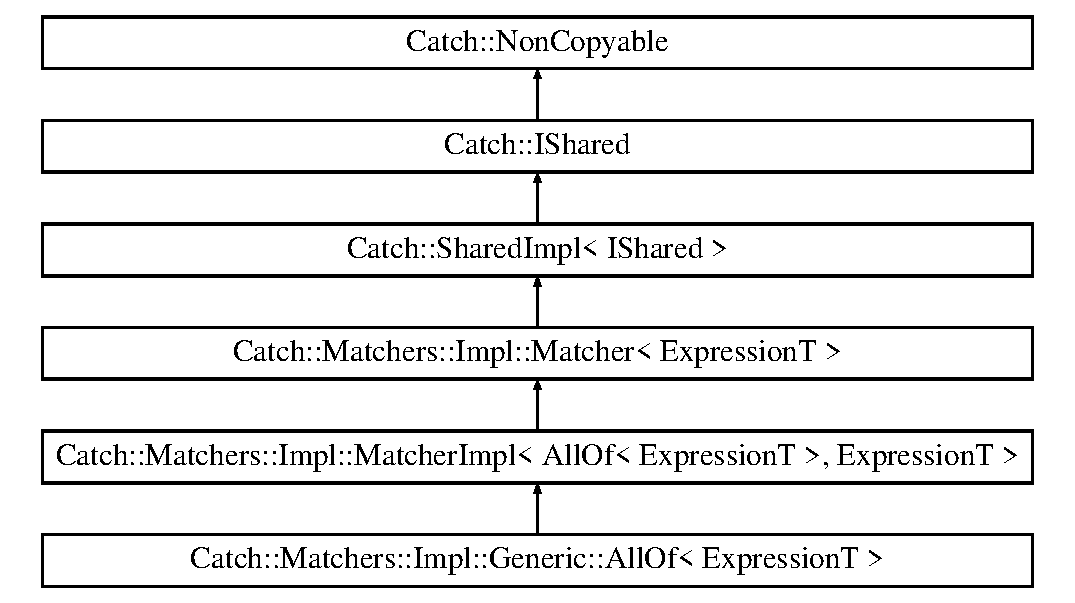
\includegraphics[height=6.000000cm]{class_catch_1_1_matchers_1_1_impl_1_1_generic_1_1_all_of}
\end{center}
\end{figure}
\subsection*{Public Member Functions}
\begin{DoxyCompactItemize}
\item 
\mbox{\Hypertarget{class_catch_1_1_matchers_1_1_impl_1_1_generic_1_1_all_of_a31f7c5e570e79bdf64064ee87c331a59}\label{class_catch_1_1_matchers_1_1_impl_1_1_generic_1_1_all_of_a31f7c5e570e79bdf64064ee87c331a59}} 
{\bfseries All\+Of} (\hyperlink{class_catch_1_1_matchers_1_1_impl_1_1_generic_1_1_all_of}{All\+Of} const \&other)
\item 
\mbox{\Hypertarget{class_catch_1_1_matchers_1_1_impl_1_1_generic_1_1_all_of_a8c5cd1e494ab697076da418ee72ac297}\label{class_catch_1_1_matchers_1_1_impl_1_1_generic_1_1_all_of_a8c5cd1e494ab697076da418ee72ac297}} 
\hyperlink{class_catch_1_1_matchers_1_1_impl_1_1_generic_1_1_all_of}{All\+Of} \& {\bfseries add} (\hyperlink{struct_catch_1_1_matchers_1_1_impl_1_1_matcher}{Matcher}$<$ ExpressionT $>$ const \&matcher)
\item 
\mbox{\Hypertarget{class_catch_1_1_matchers_1_1_impl_1_1_generic_1_1_all_of_a95231b6a455e1a646d0b54bce55138be}\label{class_catch_1_1_matchers_1_1_impl_1_1_generic_1_1_all_of_a95231b6a455e1a646d0b54bce55138be}} 
virtual bool {\bfseries match} (ExpressionT const \&expr) const
\item 
\mbox{\Hypertarget{class_catch_1_1_matchers_1_1_impl_1_1_generic_1_1_all_of_a8c8e7742501dc81e51a3c745d6f74119}\label{class_catch_1_1_matchers_1_1_impl_1_1_generic_1_1_all_of_a8c8e7742501dc81e51a3c745d6f74119}} 
virtual \textbf{ std\+::string} {\bfseries to\+String} () const
\item 
\mbox{\Hypertarget{class_catch_1_1_matchers_1_1_impl_1_1_generic_1_1_all_of_aca6497aaa7fdb6560ebe850f32ccbf15}\label{class_catch_1_1_matchers_1_1_impl_1_1_generic_1_1_all_of_aca6497aaa7fdb6560ebe850f32ccbf15}} 
\hyperlink{class_catch_1_1_matchers_1_1_impl_1_1_generic_1_1_all_of}{All\+Of} {\bfseries operator\&\&} (\hyperlink{struct_catch_1_1_matchers_1_1_impl_1_1_matcher}{Matcher}$<$ ExpressionT $>$ const \&other) const
\end{DoxyCompactItemize}
\subsection*{Additional Inherited Members}


\subsection{Detailed Description}
\subsubsection*{template$<$typename ExpressionT$>$\newline
class Catch\+::\+Matchers\+::\+Impl\+::\+Generic\+::\+All\+Of$<$ Expression\+T $>$}



Definition at line 852 of file catch.\+hpp.



The documentation for this class was generated from the following file\+:\begin{DoxyCompactItemize}
\item 
Tests/catch.\+hpp\end{DoxyCompactItemize}

\hypertarget{class_catch_1_1_matchers_1_1_impl_1_1_generic_1_1_any_of}{}\section{Catch\+:\+:Matchers\+:\+:Impl\+:\+:Generic\+:\+:Any\+Of$<$ ExpressionT $>$ Class Template Reference}
\label{class_catch_1_1_matchers_1_1_impl_1_1_generic_1_1_any_of}\index{Catch\+::\+Matchers\+::\+Impl\+::\+Generic\+::\+Any\+Of$<$ Expression\+T $>$@{Catch\+::\+Matchers\+::\+Impl\+::\+Generic\+::\+Any\+Of$<$ Expression\+T $>$}}
Inheritance diagram for Catch\+:\+:Matchers\+:\+:Impl\+:\+:Generic\+:\+:Any\+Of$<$ ExpressionT $>$\+:\begin{figure}[H]
\begin{center}
\leavevmode
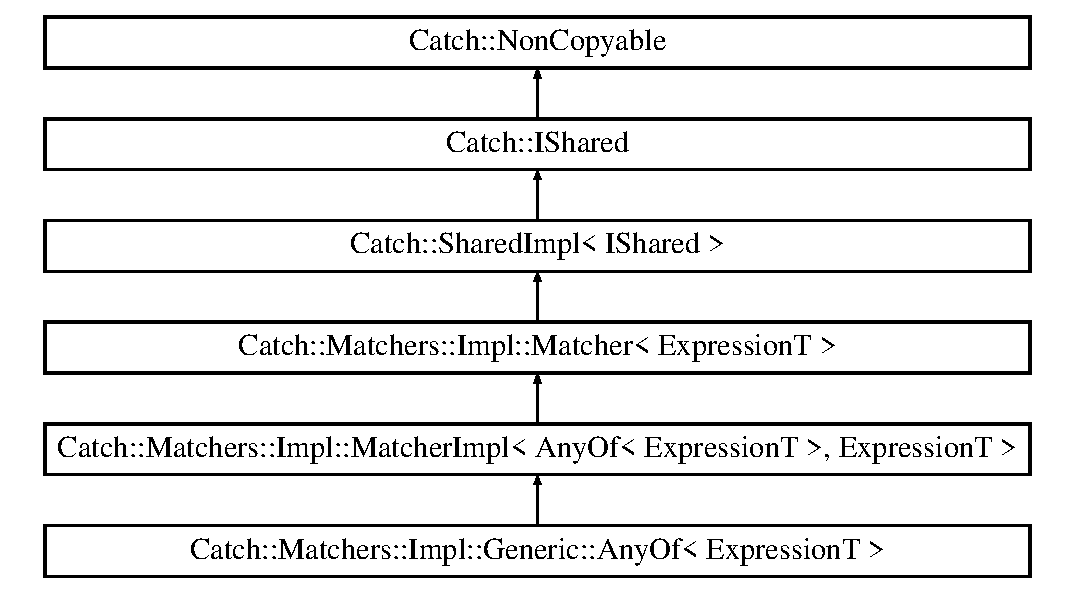
\includegraphics[height=6.000000cm]{class_catch_1_1_matchers_1_1_impl_1_1_generic_1_1_any_of}
\end{center}
\end{figure}
\subsection*{Public Member Functions}
\begin{DoxyCompactItemize}
\item 
\mbox{\Hypertarget{class_catch_1_1_matchers_1_1_impl_1_1_generic_1_1_any_of_a74fbc05b32d334fcbfd0fae0163a404e}\label{class_catch_1_1_matchers_1_1_impl_1_1_generic_1_1_any_of_a74fbc05b32d334fcbfd0fae0163a404e}} 
{\bfseries Any\+Of} (\hyperlink{class_catch_1_1_matchers_1_1_impl_1_1_generic_1_1_any_of}{Any\+Of} const \&other)
\item 
\mbox{\Hypertarget{class_catch_1_1_matchers_1_1_impl_1_1_generic_1_1_any_of_a3bce94b627551e5f96c5f9c6060413f0}\label{class_catch_1_1_matchers_1_1_impl_1_1_generic_1_1_any_of_a3bce94b627551e5f96c5f9c6060413f0}} 
\hyperlink{class_catch_1_1_matchers_1_1_impl_1_1_generic_1_1_any_of}{Any\+Of} \& {\bfseries add} (\hyperlink{struct_catch_1_1_matchers_1_1_impl_1_1_matcher}{Matcher}$<$ ExpressionT $>$ const \&matcher)
\item 
\mbox{\Hypertarget{class_catch_1_1_matchers_1_1_impl_1_1_generic_1_1_any_of_adebd5437cdb8e0d54e16e97fe26e7e85}\label{class_catch_1_1_matchers_1_1_impl_1_1_generic_1_1_any_of_adebd5437cdb8e0d54e16e97fe26e7e85}} 
virtual bool {\bfseries match} (ExpressionT const \&expr) const
\item 
\mbox{\Hypertarget{class_catch_1_1_matchers_1_1_impl_1_1_generic_1_1_any_of_a331aaf012b133682eadc9ed5342f848a}\label{class_catch_1_1_matchers_1_1_impl_1_1_generic_1_1_any_of_a331aaf012b133682eadc9ed5342f848a}} 
virtual \textbf{ std\+::string} {\bfseries to\+String} () const
\item 
\mbox{\Hypertarget{class_catch_1_1_matchers_1_1_impl_1_1_generic_1_1_any_of_a6dc9aee9a816f66ddc9de0c45c1c9ac1}\label{class_catch_1_1_matchers_1_1_impl_1_1_generic_1_1_any_of_a6dc9aee9a816f66ddc9de0c45c1c9ac1}} 
\hyperlink{class_catch_1_1_matchers_1_1_impl_1_1_generic_1_1_any_of}{Any\+Of} {\bfseries operator$\vert$$\vert$} (\hyperlink{struct_catch_1_1_matchers_1_1_impl_1_1_matcher}{Matcher}$<$ ExpressionT $>$ const \&other) const
\end{DoxyCompactItemize}
\subsection*{Additional Inherited Members}


\subsection{Detailed Description}
\subsubsection*{template$<$typename ExpressionT$>$\newline
class Catch\+::\+Matchers\+::\+Impl\+::\+Generic\+::\+Any\+Of$<$ Expression\+T $>$}



Definition at line 853 of file catch.\+hpp.



The documentation for this class was generated from the following file\+:\begin{DoxyCompactItemize}
\item 
Tests/catch.\+hpp\end{DoxyCompactItemize}

\hypertarget{class_catch_1_1_detail_1_1_approx}{}\section{Catch\+:\+:Detail\+:\+:Approx Class Reference}
\label{class_catch_1_1_detail_1_1_approx}\index{Catch\+::\+Detail\+::\+Approx@{Catch\+::\+Detail\+::\+Approx}}
\subsection*{Public Member Functions}
\begin{DoxyCompactItemize}
\item 
\mbox{\Hypertarget{class_catch_1_1_detail_1_1_approx_a1a8618ea8db08c66bd3d9fe8f74b957a}\label{class_catch_1_1_detail_1_1_approx_a1a8618ea8db08c66bd3d9fe8f74b957a}} 
{\bfseries Approx} (double value)
\item 
\mbox{\Hypertarget{class_catch_1_1_detail_1_1_approx_a807330c63266fc914abdf6e461255a54}\label{class_catch_1_1_detail_1_1_approx_a807330c63266fc914abdf6e461255a54}} 
{\bfseries Approx} (\hyperlink{class_catch_1_1_detail_1_1_approx}{Approx} const \&other)
\item 
\mbox{\Hypertarget{class_catch_1_1_detail_1_1_approx_a48c9cbc28a05dc9dc8c3973b9eae2268}\label{class_catch_1_1_detail_1_1_approx_a48c9cbc28a05dc9dc8c3973b9eae2268}} 
\hyperlink{class_catch_1_1_detail_1_1_approx}{Approx} {\bfseries operator()} (double value)
\item 
\mbox{\Hypertarget{class_catch_1_1_detail_1_1_approx_a05c50c3ad0a971fab19345b5d94979a9}\label{class_catch_1_1_detail_1_1_approx_a05c50c3ad0a971fab19345b5d94979a9}} 
\hyperlink{class_catch_1_1_detail_1_1_approx}{Approx} \& {\bfseries epsilon} (double new\+Epsilon)
\item 
\mbox{\Hypertarget{class_catch_1_1_detail_1_1_approx_acd80f0737bf38112beacd5ca95bef113}\label{class_catch_1_1_detail_1_1_approx_acd80f0737bf38112beacd5ca95bef113}} 
\hyperlink{class_catch_1_1_detail_1_1_approx}{Approx} \& {\bfseries scale} (double new\+Scale)
\item 
\mbox{\Hypertarget{class_catch_1_1_detail_1_1_approx_a972fd9ac60607483263f1b0f0f9955e6}\label{class_catch_1_1_detail_1_1_approx_a972fd9ac60607483263f1b0f0f9955e6}} 
\textbf{ std\+::string} {\bfseries to\+String} () const
\end{DoxyCompactItemize}
\subsection*{Static Public Member Functions}
\begin{DoxyCompactItemize}
\item 
\mbox{\Hypertarget{class_catch_1_1_detail_1_1_approx_aaf86dc0ee92272ac2d9839197a07951d}\label{class_catch_1_1_detail_1_1_approx_aaf86dc0ee92272ac2d9839197a07951d}} 
static \hyperlink{class_catch_1_1_detail_1_1_approx}{Approx} {\bfseries custom} ()
\end{DoxyCompactItemize}
\subsection*{Friends}
\begin{DoxyCompactItemize}
\item 
\mbox{\Hypertarget{class_catch_1_1_detail_1_1_approx_ac766f044f1c63f0c5997982baefd9049}\label{class_catch_1_1_detail_1_1_approx_ac766f044f1c63f0c5997982baefd9049}} 
bool {\bfseries operator==} (double lhs, \hyperlink{class_catch_1_1_detail_1_1_approx}{Approx} const \&rhs)
\item 
\mbox{\Hypertarget{class_catch_1_1_detail_1_1_approx_a35999631e6cef569f9da9f3fa910db22}\label{class_catch_1_1_detail_1_1_approx_a35999631e6cef569f9da9f3fa910db22}} 
bool {\bfseries operator==} (\hyperlink{class_catch_1_1_detail_1_1_approx}{Approx} const \&lhs, double rhs)
\item 
\mbox{\Hypertarget{class_catch_1_1_detail_1_1_approx_a83b3763569a7ecc143c335b630be0e47}\label{class_catch_1_1_detail_1_1_approx_a83b3763569a7ecc143c335b630be0e47}} 
bool {\bfseries operator!=} (double lhs, \hyperlink{class_catch_1_1_detail_1_1_approx}{Approx} const \&rhs)
\item 
\mbox{\Hypertarget{class_catch_1_1_detail_1_1_approx_a7497ef839f8026cc0edd6269a80f3e09}\label{class_catch_1_1_detail_1_1_approx_a7497ef839f8026cc0edd6269a80f3e09}} 
bool {\bfseries operator!=} (\hyperlink{class_catch_1_1_detail_1_1_approx}{Approx} const \&lhs, double rhs)
\end{DoxyCompactItemize}


\subsection{Detailed Description}


Definition at line 2580 of file catch.\+hpp.



The documentation for this class was generated from the following file\+:\begin{DoxyCompactItemize}
\item 
Tests/catch.\+hpp\end{DoxyCompactItemize}

\hypertarget{struct_catch_1_1_assertion_info}{}\section{Catch\+:\+:Assertion\+Info Struct Reference}
\label{struct_catch_1_1_assertion_info}\index{Catch\+::\+Assertion\+Info@{Catch\+::\+Assertion\+Info}}
\subsection*{Public Member Functions}
\begin{DoxyCompactItemize}
\item 
\mbox{\Hypertarget{struct_catch_1_1_assertion_info_aaf6cc3eebd40391e54d37ed42953c73f}\label{struct_catch_1_1_assertion_info_aaf6cc3eebd40391e54d37ed42953c73f}} 
{\bfseries Assertion\+Info} (\textbf{ std\+::string} const \&\+\_\+macro\+Name, \hyperlink{struct_catch_1_1_source_line_info}{Source\+Line\+Info} const \&\+\_\+line\+Info, \textbf{ std\+::string} const \&\+\_\+captured\+Expression, Result\+Disposition\+::\+Flags \+\_\+result\+Disposition)
\end{DoxyCompactItemize}
\subsection*{Public Attributes}
\begin{DoxyCompactItemize}
\item 
\mbox{\Hypertarget{struct_catch_1_1_assertion_info_ac2e59e8c89e00eb3390768f50d540b18}\label{struct_catch_1_1_assertion_info_ac2e59e8c89e00eb3390768f50d540b18}} 
\textbf{ std\+::string} {\bfseries macro\+Name}
\item 
\mbox{\Hypertarget{struct_catch_1_1_assertion_info_a17bdbb404ba12658034f833be2f4c3e7}\label{struct_catch_1_1_assertion_info_a17bdbb404ba12658034f833be2f4c3e7}} 
\hyperlink{struct_catch_1_1_source_line_info}{Source\+Line\+Info} {\bfseries line\+Info}
\item 
\mbox{\Hypertarget{struct_catch_1_1_assertion_info_af7c1d3cbfa346e9a303030fa0ef0cb54}\label{struct_catch_1_1_assertion_info_af7c1d3cbfa346e9a303030fa0ef0cb54}} 
\textbf{ std\+::string} {\bfseries captured\+Expression}
\item 
\mbox{\Hypertarget{struct_catch_1_1_assertion_info_a60353b3632ab2f827162f2b2d6911073}\label{struct_catch_1_1_assertion_info_a60353b3632ab2f827162f2b2d6911073}} 
Result\+Disposition\+::\+Flags {\bfseries result\+Disposition}
\end{DoxyCompactItemize}


\subsection{Detailed Description}


Definition at line 789 of file catch.\+hpp.



The documentation for this struct was generated from the following file\+:\begin{DoxyCompactItemize}
\item 
Tests/catch.\+hpp\end{DoxyCompactItemize}

\hypertarget{class_catch_1_1_assertion_result}{}\section{Catch\+:\+:Assertion\+Result Class Reference}
\label{class_catch_1_1_assertion_result}\index{Catch\+::\+Assertion\+Result@{Catch\+::\+Assertion\+Result}}
\subsection*{Public Member Functions}
\begin{DoxyCompactItemize}
\item 
\mbox{\Hypertarget{class_catch_1_1_assertion_result_ab58aeec27052ba400633ed0e36cea692}\label{class_catch_1_1_assertion_result_ab58aeec27052ba400633ed0e36cea692}} 
{\bfseries Assertion\+Result} (\hyperlink{struct_catch_1_1_assertion_info}{Assertion\+Info} const \&info, \hyperlink{struct_catch_1_1_assertion_result_data}{Assertion\+Result\+Data} const \&data)
\item 
\mbox{\Hypertarget{class_catch_1_1_assertion_result_ae39658b71c4afc3c8a859043b0e97027}\label{class_catch_1_1_assertion_result_ae39658b71c4afc3c8a859043b0e97027}} 
bool {\bfseries is\+Ok} () const
\item 
\mbox{\Hypertarget{class_catch_1_1_assertion_result_ac5cc872b721d5fb65d87221d30b22fdd}\label{class_catch_1_1_assertion_result_ac5cc872b721d5fb65d87221d30b22fdd}} 
bool {\bfseries succeeded} () const
\item 
\mbox{\Hypertarget{class_catch_1_1_assertion_result_ac810750194e1722489d2fd16e8c6a4a8}\label{class_catch_1_1_assertion_result_ac810750194e1722489d2fd16e8c6a4a8}} 
Result\+Was\+::\+Of\+Type {\bfseries get\+Result\+Type} () const
\item 
\mbox{\Hypertarget{class_catch_1_1_assertion_result_aba37b4fef1015989df2136592958e984}\label{class_catch_1_1_assertion_result_aba37b4fef1015989df2136592958e984}} 
bool {\bfseries has\+Expression} () const
\item 
\mbox{\Hypertarget{class_catch_1_1_assertion_result_aae37064b401919fa8ac480ef86cca924}\label{class_catch_1_1_assertion_result_aae37064b401919fa8ac480ef86cca924}} 
bool {\bfseries has\+Message} () const
\item 
\mbox{\Hypertarget{class_catch_1_1_assertion_result_a26a777f3959353c729544cb2ace0d279}\label{class_catch_1_1_assertion_result_a26a777f3959353c729544cb2ace0d279}} 
\textbf{ std\+::string} {\bfseries get\+Expression} () const
\item 
\mbox{\Hypertarget{class_catch_1_1_assertion_result_aac35a0ca42d33bff6467c76573730f5e}\label{class_catch_1_1_assertion_result_aac35a0ca42d33bff6467c76573730f5e}} 
\textbf{ std\+::string} {\bfseries get\+Expression\+In\+Macro} () const
\item 
\mbox{\Hypertarget{class_catch_1_1_assertion_result_a78c43506c2b3d8cc1fb141a97d09ec94}\label{class_catch_1_1_assertion_result_a78c43506c2b3d8cc1fb141a97d09ec94}} 
bool {\bfseries has\+Expanded\+Expression} () const
\item 
\mbox{\Hypertarget{class_catch_1_1_assertion_result_aaa46070791a6c07caaed86229b8d9d75}\label{class_catch_1_1_assertion_result_aaa46070791a6c07caaed86229b8d9d75}} 
\textbf{ std\+::string} {\bfseries get\+Expanded\+Expression} () const
\item 
\mbox{\Hypertarget{class_catch_1_1_assertion_result_ae730943beed46921b09383c673e35786}\label{class_catch_1_1_assertion_result_ae730943beed46921b09383c673e35786}} 
\textbf{ std\+::string} {\bfseries get\+Message} () const
\item 
\mbox{\Hypertarget{class_catch_1_1_assertion_result_aa4d3fdbfe276a69a035762dbb790800f}\label{class_catch_1_1_assertion_result_aa4d3fdbfe276a69a035762dbb790800f}} 
\hyperlink{struct_catch_1_1_source_line_info}{Source\+Line\+Info} {\bfseries get\+Source\+Info} () const
\item 
\mbox{\Hypertarget{class_catch_1_1_assertion_result_aaefd9a0384282fd08a4a72aa19bd0628}\label{class_catch_1_1_assertion_result_aaefd9a0384282fd08a4a72aa19bd0628}} 
\textbf{ std\+::string} {\bfseries get\+Test\+Macro\+Name} () const
\end{DoxyCompactItemize}
\subsection*{Protected Attributes}
\begin{DoxyCompactItemize}
\item 
\mbox{\Hypertarget{class_catch_1_1_assertion_result_a3e7236f73a51d6fc8bb9dfdefcee7772}\label{class_catch_1_1_assertion_result_a3e7236f73a51d6fc8bb9dfdefcee7772}} 
\hyperlink{struct_catch_1_1_assertion_info}{Assertion\+Info} {\bfseries m\+\_\+info}
\item 
\mbox{\Hypertarget{class_catch_1_1_assertion_result_add3455b8bbedb0d643e18da67c66b4f7}\label{class_catch_1_1_assertion_result_add3455b8bbedb0d643e18da67c66b4f7}} 
\hyperlink{struct_catch_1_1_assertion_result_data}{Assertion\+Result\+Data} {\bfseries m\+\_\+result\+Data}
\end{DoxyCompactItemize}


\subsection{Detailed Description}


Definition at line 812 of file catch.\+hpp.



The documentation for this class was generated from the following file\+:\begin{DoxyCompactItemize}
\item 
Tests/catch.\+hpp\end{DoxyCompactItemize}

\hypertarget{struct_catch_1_1_assertion_result_data}{}\section{Catch\+:\+:Assertion\+Result\+Data Struct Reference}
\label{struct_catch_1_1_assertion_result_data}\index{Catch\+::\+Assertion\+Result\+Data@{Catch\+::\+Assertion\+Result\+Data}}
\subsection*{Public Attributes}
\begin{DoxyCompactItemize}
\item 
\mbox{\Hypertarget{struct_catch_1_1_assertion_result_data_a9e809d36fffbeb1c7d0cbe7382dd9595}\label{struct_catch_1_1_assertion_result_data_a9e809d36fffbeb1c7d0cbe7382dd9595}} 
\textbf{ std\+::string} {\bfseries reconstructed\+Expression}
\item 
\mbox{\Hypertarget{struct_catch_1_1_assertion_result_data_ac34215803c4c4a88f795879f61c1f7b4}\label{struct_catch_1_1_assertion_result_data_ac34215803c4c4a88f795879f61c1f7b4}} 
\textbf{ std\+::string} {\bfseries message}
\item 
\mbox{\Hypertarget{struct_catch_1_1_assertion_result_data_a7ceab4a7ff722aec5587e3748caf66b7}\label{struct_catch_1_1_assertion_result_data_a7ceab4a7ff722aec5587e3748caf66b7}} 
Result\+Was\+::\+Of\+Type {\bfseries result\+Type}
\end{DoxyCompactItemize}


\subsection{Detailed Description}


Definition at line 803 of file catch.\+hpp.



The documentation for this struct was generated from the following file\+:\begin{DoxyCompactItemize}
\item 
Tests/catch.\+hpp\end{DoxyCompactItemize}

\hypertarget{struct_catch_1_1_auto_reg}{}\section{Catch\+:\+:Auto\+Reg Struct Reference}
\label{struct_catch_1_1_auto_reg}\index{Catch\+::\+Auto\+Reg@{Catch\+::\+Auto\+Reg}}
\subsection*{Public Member Functions}
\begin{DoxyCompactItemize}
\item 
\mbox{\Hypertarget{struct_catch_1_1_auto_reg_af224f4568d57b8652474df475a164a8c}\label{struct_catch_1_1_auto_reg_af224f4568d57b8652474df475a164a8c}} 
{\bfseries Auto\+Reg} (Test\+Function function, \hyperlink{struct_catch_1_1_source_line_info}{Source\+Line\+Info} const \&line\+Info, \hyperlink{struct_catch_1_1_name_and_desc}{Name\+And\+Desc} const \&name\+And\+Desc)
\item 
\mbox{\Hypertarget{struct_catch_1_1_auto_reg_a1bf9207fe0a02b46dc0ab1cc03cbe738}\label{struct_catch_1_1_auto_reg_a1bf9207fe0a02b46dc0ab1cc03cbe738}} 
{\footnotesize template$<$typename C $>$ }\\{\bfseries Auto\+Reg} (void(C\+::$\ast$method)(), char const $\ast$class\+Name, \hyperlink{struct_catch_1_1_name_and_desc}{Name\+And\+Desc} const \&name\+And\+Desc, \hyperlink{struct_catch_1_1_source_line_info}{Source\+Line\+Info} const \&line\+Info)
\end{DoxyCompactItemize}


\subsection{Detailed Description}


Definition at line 638 of file catch.\+hpp.



The documentation for this struct was generated from the following file\+:\begin{DoxyCompactItemize}
\item 
Tests/catch.\+hpp\end{DoxyCompactItemize}

\hypertarget{class_catch_1_1_between_generator}{}\section{Catch\+:\+:Between\+Generator$<$ T $>$ Class Template Reference}
\label{class_catch_1_1_between_generator}\index{Catch\+::\+Between\+Generator$<$ T $>$@{Catch\+::\+Between\+Generator$<$ T $>$}}
Inheritance diagram for Catch\+:\+:Between\+Generator$<$ T $>$\+:\begin{figure}[H]
\begin{center}
\leavevmode
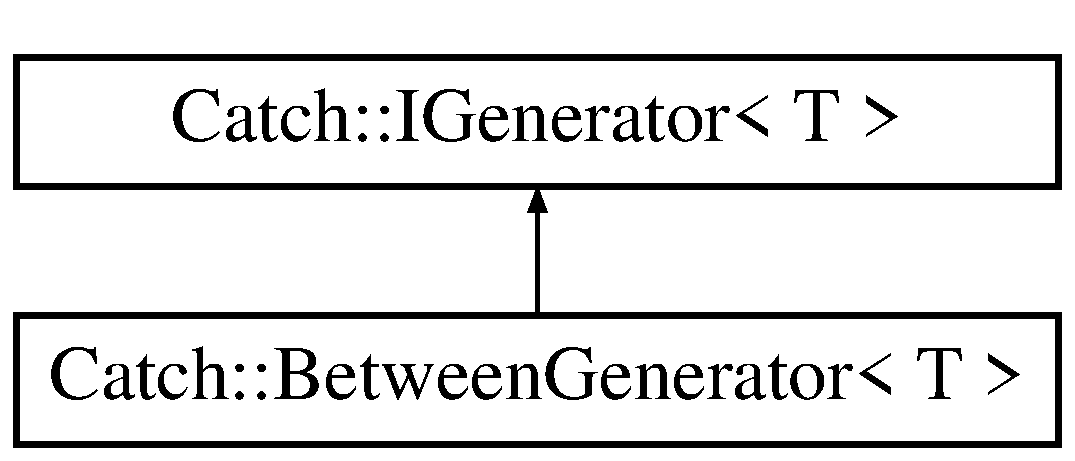
\includegraphics[height=2.000000cm]{class_catch_1_1_between_generator}
\end{center}
\end{figure}
\subsection*{Public Member Functions}
\begin{DoxyCompactItemize}
\item 
\mbox{\Hypertarget{class_catch_1_1_between_generator_a835a057d691ae37caef660624099b51c}\label{class_catch_1_1_between_generator_a835a057d691ae37caef660624099b51c}} 
{\bfseries Between\+Generator} (T from, T to)
\item 
\mbox{\Hypertarget{class_catch_1_1_between_generator_a913f74bb0c23b3bc0127abfffdabbd94}\label{class_catch_1_1_between_generator_a913f74bb0c23b3bc0127abfffdabbd94}} 
virtual T {\bfseries get\+Value} (\textbf{ std\+::size\+\_\+t} index) const
\item 
\mbox{\Hypertarget{class_catch_1_1_between_generator_af65a1fe51f9b1106fc676e3dd189adb6}\label{class_catch_1_1_between_generator_af65a1fe51f9b1106fc676e3dd189adb6}} 
virtual \textbf{ std\+::size\+\_\+t} {\bfseries size} () const
\end{DoxyCompactItemize}


\subsection{Detailed Description}
\subsubsection*{template$<$typename T$>$\newline
class Catch\+::\+Between\+Generator$<$ T $>$}



Definition at line 2308 of file catch.\+hpp.



The documentation for this class was generated from the following file\+:\begin{DoxyCompactItemize}
\item 
Tests/catch.\+hpp\end{DoxyCompactItemize}

\hypertarget{class_board}{}\section{Board Class Reference}
\label{class_board}\index{Board@{Board}}


The \hyperlink{class_board}{Board} class This class represents a board.  




{\ttfamily \#include $<$board.\+h$>$}

\subsection*{Public Member Functions}
\begin{DoxyCompactItemize}
\item 
\hyperlink{class_board_ad42b2461203bc38788e8f3488a6a7636}{Board} (const \hyperlink{struct_board_type}{Board\+Type} \&btype)
\begin{DoxyCompactList}\small\item\em the constructor It creates an instance of the class using a predefined \hyperlink{struct_board_type}{Board\+Type}. \end{DoxyCompactList}\item 
\mbox{\Hypertarget{class_board_ae87b63aa7c19a7ef82f6d70cbb9c7646}\label{class_board_ae87b63aa7c19a7ef82f6d70cbb9c7646}} 
\hyperlink{class_board_ae87b63aa7c19a7ef82f6d70cbb9c7646}{Board} ()=default
\begin{DoxyCompactList}\small\item\em the constructor It creates an instance of the class from nothing. \end{DoxyCompactList}\item 
\mbox{\Hypertarget{class_board_af73f45730119a1fd8f6670f53f959e68}\label{class_board_af73f45730119a1fd8f6670f53f959e68}} 
\hyperlink{class_board_af73f45730119a1fd8f6670f53f959e68}{$\sim$\+Board} ()
\begin{DoxyCompactList}\small\item\em the destructor It deletes all the elements from \hyperlink{class_board}{Board} that need to be deleted. \end{DoxyCompactList}\item 
void \hyperlink{class_board_a5667cea4135532fa7666bf7f5cf6e71b}{set\+Board\+Type} (\hyperlink{struct_board_type}{Board\+Type} btype)
\begin{DoxyCompactList}\small\item\em the setter of \hyperlink{struct_board_type}{Board\+Type}. Changes the values of the \hyperlink{struct_board_type}{Board\+Type} with the value of the one in parameter. \end{DoxyCompactList}\item 
\hyperlink{struct_board_type}{Board\+Type} \& \hyperlink{class_board_a30189580d1e2627fc32b40a33db9c5a5}{get\+Board\+Type} ()
\begin{DoxyCompactList}\small\item\em the getter of \hyperlink{struct_board_type}{Board\+Type}. Returns the \hyperlink{struct_board_type}{Board\+Type}. \end{DoxyCompactList}\item 
\textbf{ std\+::vector}$<$ \textbf{ std\+::vector}$<$ \hyperlink{class_case}{Case} $>$ $>$ \& \hyperlink{class_board_af801e2935f37e23a3714d034e231a5ba}{get\+Board} ()
\begin{DoxyCompactList}\small\item\em the getter of the board. Returns the board. \end{DoxyCompactList}\item 
\mbox{\Hypertarget{class_board_a305b154a3ac53d119fc78efe053f4745}\label{class_board_a305b154a3ac53d119fc78efe053f4745}} 
void \hyperlink{class_board_a305b154a3ac53d119fc78efe053f4745}{unveil\+All} ()
\begin{DoxyCompactList}\small\item\em unveill all the cases of the board. It sets to visible all the cases. \end{DoxyCompactList}\item 
void \hyperlink{class_board_a182d0e797d7482a9091989b16dbcbee9}{set\+Bombs\+In\+Table} (int col, int row)
\begin{DoxyCompactList}\small\item\em puts all the bombs in the board. It randomly chooses X cases, X being the number of bombs, and puts a bomb on them. The case defined by col and row can not contain a bomb. \end{DoxyCompactList}\item 
\mbox{\Hypertarget{class_board_ada048789b3d9e13aaa52f4b8d1a72b50}\label{class_board_ada048789b3d9e13aaa52f4b8d1a72b50}} 
void \hyperlink{class_board_ada048789b3d9e13aaa52f4b8d1a72b50}{fill\+Board} ()
\begin{DoxyCompactList}\small\item\em fills all the case of the square that does not contain a bomb. Those have been previously filled. So it will set the content of the different cases. The content represents the number of bombs that are around those cases. \end{DoxyCompactList}\item 
bool \hyperlink{class_board_a472731150e19ecdd2d71bcc098037eb8}{is\+Won} ()
\begin{DoxyCompactList}\small\item\em states if the game is won. It is won if all the non-\/bomb cases are unveiled. \end{DoxyCompactList}\item 
void \hyperlink{class_board_a1d4e828a0cc3b85ba3f86534e76e2f84}{put\+Flag} (int i, int j)
\begin{DoxyCompactList}\small\item\em puts a flag on the case indicated by i and j. \end{DoxyCompactList}\item 
bool \hyperlink{class_board_a47700b8c7c08c2843e200594e620f2fa}{play} (int i, int j)
\begin{DoxyCompactList}\small\item\em unveil the case indicated by i and j. \end{DoxyCompactList}\item 
\hyperlink{class_case}{Case} \hyperlink{class_board_a66b4889df2323241f10aca4b1d38bdf5}{activate\+Bonus} ()
\begin{DoxyCompactList}\small\item\em activate\+Bonus Selects randomly a case that will be unveil for the user. \end{DoxyCompactList}\end{DoxyCompactItemize}


\subsection{Detailed Description}
The \hyperlink{class_board}{Board} class This class represents a board. 

Definition at line 12 of file board.\+h.



\subsection{Constructor \& Destructor Documentation}
\mbox{\Hypertarget{class_board_ad42b2461203bc38788e8f3488a6a7636}\label{class_board_ad42b2461203bc38788e8f3488a6a7636}} 
\index{Board@{Board}!Board@{Board}}
\index{Board@{Board}!Board@{Board}}
\subsubsection{\texorpdfstring{Board()}{Board()}}
{\footnotesize\ttfamily Board\+::\+Board (\begin{DoxyParamCaption}\item[{const \hyperlink{struct_board_type}{Board\+Type} \&}]{btype }\end{DoxyParamCaption})}



the constructor It creates an instance of the class using a predefined \hyperlink{struct_board_type}{Board\+Type}. 


\begin{DoxyParams}{Parameters}
{\em btype} & the type of the board. \\
\hline
\end{DoxyParams}


Definition at line 11 of file board.\+cpp.



\subsection{Member Function Documentation}
\mbox{\Hypertarget{class_board_a66b4889df2323241f10aca4b1d38bdf5}\label{class_board_a66b4889df2323241f10aca4b1d38bdf5}} 
\index{Board@{Board}!activate\+Bonus@{activate\+Bonus}}
\index{activate\+Bonus@{activate\+Bonus}!Board@{Board}}
\subsubsection{\texorpdfstring{activate\+Bonus()}{activateBonus()}}
{\footnotesize\ttfamily \hyperlink{class_case}{Case} Board\+::activate\+Bonus (\begin{DoxyParamCaption}{ }\end{DoxyParamCaption})}



activate\+Bonus Selects randomly a case that will be unveil for the user. 

\begin{DoxyReturn}{Returns}
the case which the computer will reveal for the user. 
\end{DoxyReturn}


Definition at line 191 of file board.\+cpp.

\mbox{\Hypertarget{class_board_af801e2935f37e23a3714d034e231a5ba}\label{class_board_af801e2935f37e23a3714d034e231a5ba}} 
\index{Board@{Board}!get\+Board@{get\+Board}}
\index{get\+Board@{get\+Board}!Board@{Board}}
\subsubsection{\texorpdfstring{get\+Board()}{getBoard()}}
{\footnotesize\ttfamily \textbf{ std\+::vector}$<$ \textbf{ std\+::vector}$<$ \hyperlink{class_case}{Case} $>$ $>$ \& Board\+::get\+Board (\begin{DoxyParamCaption}{ }\end{DoxyParamCaption})\hspace{0.3cm}{\ttfamily [inline]}}



the getter of the board. Returns the board. 

\begin{DoxyReturn}{Returns}
a vector of \hyperlink{class_case}{Case}. 
\end{DoxyReturn}


Definition at line 130 of file board.\+h.

\mbox{\Hypertarget{class_board_a30189580d1e2627fc32b40a33db9c5a5}\label{class_board_a30189580d1e2627fc32b40a33db9c5a5}} 
\index{Board@{Board}!get\+Board\+Type@{get\+Board\+Type}}
\index{get\+Board\+Type@{get\+Board\+Type}!Board@{Board}}
\subsubsection{\texorpdfstring{get\+Board\+Type()}{getBoardType()}}
{\footnotesize\ttfamily \hyperlink{struct_board_type}{Board\+Type} \& Board\+::get\+Board\+Type (\begin{DoxyParamCaption}{ }\end{DoxyParamCaption})\hspace{0.3cm}{\ttfamily [inline]}}



the getter of \hyperlink{struct_board_type}{Board\+Type}. Returns the \hyperlink{struct_board_type}{Board\+Type}. 

\begin{DoxyReturn}{Returns}
a \hyperlink{struct_board_type}{Board\+Type}. 
\end{DoxyReturn}


Definition at line 138 of file board.\+h.

\mbox{\Hypertarget{class_board_a472731150e19ecdd2d71bcc098037eb8}\label{class_board_a472731150e19ecdd2d71bcc098037eb8}} 
\index{Board@{Board}!is\+Won@{is\+Won}}
\index{is\+Won@{is\+Won}!Board@{Board}}
\subsubsection{\texorpdfstring{is\+Won()}{isWon()}}
{\footnotesize\ttfamily bool Board\+::is\+Won (\begin{DoxyParamCaption}{ }\end{DoxyParamCaption})}



states if the game is won. It is won if all the non-\/bomb cases are unveiled. 

\begin{DoxyReturn}{Returns}
true if it is won, false otherweise. 
\end{DoxyReturn}


Definition at line 150 of file board.\+cpp.

\mbox{\Hypertarget{class_board_a47700b8c7c08c2843e200594e620f2fa}\label{class_board_a47700b8c7c08c2843e200594e620f2fa}} 
\index{Board@{Board}!play@{play}}
\index{play@{play}!Board@{Board}}
\subsubsection{\texorpdfstring{play()}{play()}}
{\footnotesize\ttfamily bool Board\+::play (\begin{DoxyParamCaption}\item[{int}]{i,  }\item[{int}]{j }\end{DoxyParamCaption})}



unveil the case indicated by i and j. 


\begin{DoxyParams}{Parameters}
{\em i} & the row. \\
\hline
{\em j} & the column. \\
\hline
\end{DoxyParams}
\begin{DoxyReturn}{Returns}
false if the case is a bomb, true otherwise. 
\end{DoxyReturn}


Definition at line 165 of file board.\+cpp.

\mbox{\Hypertarget{class_board_a1d4e828a0cc3b85ba3f86534e76e2f84}\label{class_board_a1d4e828a0cc3b85ba3f86534e76e2f84}} 
\index{Board@{Board}!put\+Flag@{put\+Flag}}
\index{put\+Flag@{put\+Flag}!Board@{Board}}
\subsubsection{\texorpdfstring{put\+Flag()}{putFlag()}}
{\footnotesize\ttfamily void Board\+::put\+Flag (\begin{DoxyParamCaption}\item[{int}]{i,  }\item[{int}]{j }\end{DoxyParamCaption})}



puts a flag on the case indicated by i and j. 


\begin{DoxyParams}{Parameters}
{\em i} & the row. \\
\hline
{\em j} & the column. \\
\hline
\end{DoxyParams}


Definition at line 138 of file board.\+cpp.

\mbox{\Hypertarget{class_board_a5667cea4135532fa7666bf7f5cf6e71b}\label{class_board_a5667cea4135532fa7666bf7f5cf6e71b}} 
\index{Board@{Board}!set\+Board\+Type@{set\+Board\+Type}}
\index{set\+Board\+Type@{set\+Board\+Type}!Board@{Board}}
\subsubsection{\texorpdfstring{set\+Board\+Type()}{setBoardType()}}
{\footnotesize\ttfamily void Board\+::set\+Board\+Type (\begin{DoxyParamCaption}\item[{\hyperlink{struct_board_type}{Board\+Type}}]{btype }\end{DoxyParamCaption})\hspace{0.3cm}{\ttfamily [inline]}}



the setter of \hyperlink{struct_board_type}{Board\+Type}. Changes the values of the \hyperlink{struct_board_type}{Board\+Type} with the value of the one in parameter. 


\begin{DoxyParams}{Parameters}
{\em btype} & the new \hyperlink{struct_board_type}{Board\+Type} from which the value are taken. \\
\hline
\end{DoxyParams}


Definition at line 134 of file board.\+h.

\mbox{\Hypertarget{class_board_a182d0e797d7482a9091989b16dbcbee9}\label{class_board_a182d0e797d7482a9091989b16dbcbee9}} 
\index{Board@{Board}!set\+Bombs\+In\+Table@{set\+Bombs\+In\+Table}}
\index{set\+Bombs\+In\+Table@{set\+Bombs\+In\+Table}!Board@{Board}}
\subsubsection{\texorpdfstring{set\+Bombs\+In\+Table()}{setBombsInTable()}}
{\footnotesize\ttfamily void Board\+::set\+Bombs\+In\+Table (\begin{DoxyParamCaption}\item[{int}]{col,  }\item[{int}]{row }\end{DoxyParamCaption})}



puts all the bombs in the board. It randomly chooses X cases, X being the number of bombs, and puts a bomb on them. The case defined by col and row can not contain a bomb. 


\begin{DoxyParams}{Parameters}
{\em col} & the given column. \\
\hline
{\em row} & the given row. \\
\hline
\end{DoxyParams}


Definition at line 108 of file board.\+cpp.



The documentation for this class was generated from the following files\+:\begin{DoxyCompactItemize}
\item 
Application/board.\+h\item 
Application/board.\+cpp\end{DoxyCompactItemize}

\hypertarget{struct_board_type}{}\section{Board\+Type Struct Reference}
\label{struct_board_type}\index{Board\+Type@{Board\+Type}}


\hyperlink{struct_board_type}{Board\+Type} A \hyperlink{struct_board_type}{Board\+Type} is composed of a \hyperlink{struct_dimension}{Dimension} and a number of bombs.  




{\ttfamily \#include $<$structure.\+h$>$}

\subsection*{Public Member Functions}
\begin{DoxyCompactItemize}
\item 
\hyperlink{struct_board_type}{Board\+Type} \& \hyperlink{struct_board_type_a9747ba7e3183a87070bf6458d3a9c976}{operator=} (const \hyperlink{struct_board_type}{Board\+Type} \&a)
\begin{DoxyCompactList}\small\item\em operator = Assigns the value of a \hyperlink{struct_board_type}{Board\+Type} to a new one. \end{DoxyCompactList}\item 
bool \hyperlink{struct_board_type_a28a88d9da8a9fdd94738d12c7192b005}{operator$<$} (const \hyperlink{struct_board_type}{Board\+Type} \&r) const
\begin{DoxyCompactList}\small\item\em operator $<$ Verifies if a \hyperlink{struct_board_type}{Board\+Type} is smaller than another. \end{DoxyCompactList}\item 
bool \hyperlink{struct_board_type_a7e193ddf65e7ce01610ecb2e88eca0d7}{operator$>$} (const \hyperlink{struct_board_type}{Board\+Type} \&r)
\begin{DoxyCompactList}\small\item\em operator $>$ Verifies if a \hyperlink{struct_board_type}{Board\+Type} is greater than another. \end{DoxyCompactList}\item 
bool \hyperlink{struct_board_type_a4a983738b8a82c018896deae60ff66dd}{operator==} (const \hyperlink{struct_board_type}{Board\+Type} \&board)
\begin{DoxyCompactList}\small\item\em operator == Verifies if two \hyperlink{struct_board_type}{Board\+Type} have the same values. \end{DoxyCompactList}\end{DoxyCompactItemize}
\subsection*{Public Attributes}
\begin{DoxyCompactItemize}
\item 
\mbox{\Hypertarget{struct_board_type_a4104dbd7195c84299197a06ae87ff4bf}\label{struct_board_type_a4104dbd7195c84299197a06ae87ff4bf}} 
\hyperlink{struct_dimension}{Dimension} \hyperlink{struct_board_type_a4104dbd7195c84299197a06ae87ff4bf}{dimension}
\begin{DoxyCompactList}\small\item\em dimension The dimension of the board. \end{DoxyCompactList}\item 
\mbox{\Hypertarget{struct_board_type_adaaa6a2f0c9049b41a53544120775286}\label{struct_board_type_adaaa6a2f0c9049b41a53544120775286}} 
int \hyperlink{struct_board_type_adaaa6a2f0c9049b41a53544120775286}{nb\+Bomb}
\begin{DoxyCompactList}\small\item\em nb\+Bomb The number of bombs that are in the board. \end{DoxyCompactList}\end{DoxyCompactItemize}


\subsection{Detailed Description}
\hyperlink{struct_board_type}{Board\+Type} A \hyperlink{struct_board_type}{Board\+Type} is composed of a \hyperlink{struct_dimension}{Dimension} and a number of bombs. 

Definition at line 123 of file structure.\+h.



\subsection{Member Function Documentation}
\mbox{\Hypertarget{struct_board_type_a28a88d9da8a9fdd94738d12c7192b005}\label{struct_board_type_a28a88d9da8a9fdd94738d12c7192b005}} 
\index{Board\+Type@{Board\+Type}!operator$<$@{operator$<$}}
\index{operator$<$@{operator$<$}!Board\+Type@{Board\+Type}}
\subsubsection{\texorpdfstring{operator$<$()}{operator<()}}
{\footnotesize\ttfamily bool Board\+Type\+::operator$<$ (\begin{DoxyParamCaption}\item[{const \hyperlink{struct_board_type}{Board\+Type} \&}]{r }\end{DoxyParamCaption}) const\hspace{0.3cm}{\ttfamily [inline]}}



operator $<$ Verifies if a \hyperlink{struct_board_type}{Board\+Type} is smaller than another. 


\begin{DoxyParams}{Parameters}
{\em a} & the \hyperlink{struct_board_type}{Board\+Type} the current \hyperlink{struct_dimension}{Dimension} is compared to. \\
\hline
\end{DoxyParams}
\begin{DoxyReturn}{Returns}
true if the \hyperlink{struct_board_type}{Board\+Type} is smaller, false otherwise. 
\end{DoxyReturn}


Definition at line 155 of file structure.\+h.

\mbox{\Hypertarget{struct_board_type_a9747ba7e3183a87070bf6458d3a9c976}\label{struct_board_type_a9747ba7e3183a87070bf6458d3a9c976}} 
\index{Board\+Type@{Board\+Type}!operator=@{operator=}}
\index{operator=@{operator=}!Board\+Type@{Board\+Type}}
\subsubsection{\texorpdfstring{operator=()}{operator=()}}
{\footnotesize\ttfamily \hyperlink{struct_board_type}{Board\+Type}\& Board\+Type\+::operator= (\begin{DoxyParamCaption}\item[{const \hyperlink{struct_board_type}{Board\+Type} \&}]{a }\end{DoxyParamCaption})\hspace{0.3cm}{\ttfamily [inline]}}



operator = Assigns the value of a \hyperlink{struct_board_type}{Board\+Type} to a new one. 


\begin{DoxyParams}{Parameters}
{\em a} & the \hyperlink{struct_board_type}{Board\+Type} we take the value from. \\
\hline
\end{DoxyParams}
\begin{DoxyReturn}{Returns}
a new \hyperlink{struct_board_type}{Board\+Type}, that has the same value as the other one. 
\end{DoxyReturn}


Definition at line 143 of file structure.\+h.

\mbox{\Hypertarget{struct_board_type_a4a983738b8a82c018896deae60ff66dd}\label{struct_board_type_a4a983738b8a82c018896deae60ff66dd}} 
\index{Board\+Type@{Board\+Type}!operator==@{operator==}}
\index{operator==@{operator==}!Board\+Type@{Board\+Type}}
\subsubsection{\texorpdfstring{operator==()}{operator==()}}
{\footnotesize\ttfamily bool Board\+Type\+::operator== (\begin{DoxyParamCaption}\item[{const \hyperlink{struct_board_type}{Board\+Type} \&}]{board }\end{DoxyParamCaption})\hspace{0.3cm}{\ttfamily [inline]}}



operator == Verifies if two \hyperlink{struct_board_type}{Board\+Type} have the same values. 


\begin{DoxyParams}{Parameters}
{\em a} & the \hyperlink{struct_board_type}{Board\+Type} the current \hyperlink{struct_dimension}{Dimension} is compared to. \\
\hline
\end{DoxyParams}
\begin{DoxyReturn}{Returns}
true if the \hyperlink{struct_board_type}{Board\+Type} are equals, false otherwise. 
\end{DoxyReturn}


Definition at line 193 of file structure.\+h.

\mbox{\Hypertarget{struct_board_type_a7e193ddf65e7ce01610ecb2e88eca0d7}\label{struct_board_type_a7e193ddf65e7ce01610ecb2e88eca0d7}} 
\index{Board\+Type@{Board\+Type}!operator$>$@{operator$>$}}
\index{operator$>$@{operator$>$}!Board\+Type@{Board\+Type}}
\subsubsection{\texorpdfstring{operator$>$()}{operator>()}}
{\footnotesize\ttfamily bool Board\+Type\+::operator$>$ (\begin{DoxyParamCaption}\item[{const \hyperlink{struct_board_type}{Board\+Type} \&}]{r }\end{DoxyParamCaption})\hspace{0.3cm}{\ttfamily [inline]}}



operator $>$ Verifies if a \hyperlink{struct_board_type}{Board\+Type} is greater than another. 


\begin{DoxyParams}{Parameters}
{\em a} & the \hyperlink{struct_board_type}{Board\+Type} the current \hyperlink{struct_dimension}{Dimension} is compared to. \\
\hline
\end{DoxyParams}
\begin{DoxyReturn}{Returns}
true if the \hyperlink{struct_board_type}{Board\+Type} is greater, false otherwise. 
\end{DoxyReturn}


Definition at line 174 of file structure.\+h.



The documentation for this struct was generated from the following file\+:\begin{DoxyCompactItemize}
\item 
Application/structure.\+h\end{DoxyCompactItemize}

\hypertarget{struct_catch_1_1_detail_1_1_borg_type}{}\section{Catch\+:\+:Detail\+:\+:Borg\+Type Struct Reference}
\label{struct_catch_1_1_detail_1_1_borg_type}\index{Catch\+::\+Detail\+::\+Borg\+Type@{Catch\+::\+Detail\+::\+Borg\+Type}}
\subsection*{Public Member Functions}
\begin{DoxyCompactItemize}
\item 
\mbox{\Hypertarget{struct_catch_1_1_detail_1_1_borg_type_a780a9946ed0d654f0bfc043c8fc505d8}\label{struct_catch_1_1_detail_1_1_borg_type_a780a9946ed0d654f0bfc043c8fc505d8}} 
{\footnotesize template$<$typename T $>$ }\\{\bfseries Borg\+Type} (T const \&)
\end{DoxyCompactItemize}


\subsection{Detailed Description}


Definition at line 1559 of file catch.\+hpp.



The documentation for this struct was generated from the following file\+:\begin{DoxyCompactItemize}
\item 
Tests/catch.\+hpp\end{DoxyCompactItemize}

\hypertarget{class_case}{}\section{Case Class Reference}
\label{class_case}\index{Case@{Case}}


The \hyperlink{class_case}{Case} class It represents a case of the board.  




{\ttfamily \#include $<$case.\+h$>$}

\subsection*{Public Member Functions}
\begin{DoxyCompactItemize}
\item 
\hyperlink{class_case_aa159b3687a5f33ef6ac7d461fa8bf948}{Case} (\hyperlink{struct_coordinates}{Coordinates} coordinates)
\begin{DoxyCompactList}\small\item\em The constructor It creates an instance of the class with predefined coordinates. \end{DoxyCompactList}\item 
\mbox{\Hypertarget{class_case_a32e1ca352eb4c7451897107758779c5d}\label{class_case_a32e1ca352eb4c7451897107758779c5d}} 
\hyperlink{class_case_a32e1ca352eb4c7451897107758779c5d}{Case} ()=default
\begin{DoxyCompactList}\small\item\em The constructor It creates an instance of the class from nothing. \end{DoxyCompactList}\item 
\mbox{\Hypertarget{class_case_ab004564aae3e15db0c7fd5dde0b4c379}\label{class_case_ab004564aae3e15db0c7fd5dde0b4c379}} 
\hyperlink{class_case_ab004564aae3e15db0c7fd5dde0b4c379}{$\sim$\+Case} ()
\begin{DoxyCompactList}\small\item\em The destructor It deletes all the element from the class that need to be deleted. \end{DoxyCompactList}\item 
\hyperlink{struct_coordinates}{Coordinates} \& \hyperlink{class_case_a6a95d5189d914c65d7a4db0f007ff533}{get\+Coordinates} ()
\begin{DoxyCompactList}\small\item\em returns the coordinates from the case \end{DoxyCompactList}\item 
bool \hyperlink{class_case_a6bf64c2cc2b5ab1ee9f340dde607eda2}{is\+Visible} ()
\begin{DoxyCompactList}\small\item\em is\+Visible indicating if a case is unveiled or not. \end{DoxyCompactList}\item 
bool \hyperlink{class_case_a9fdeaaa245f3af19ea057b93aa2b423d}{is\+Flag} ()
\begin{DoxyCompactList}\small\item\em is\+Flag indicating if a case has a flag on it. \end{DoxyCompactList}\item 
bool \hyperlink{class_case_a40789e3a7a8405f4dc8091d87ac25fd8}{is\+Bomb} ()
\begin{DoxyCompactList}\small\item\em is\+Bomb indicating if a case has a bomb on it. \end{DoxyCompactList}\item 
\mbox{\Hypertarget{class_case_a6385233b74ac590eead57c153449dff9}\label{class_case_a6385233b74ac590eead57c153449dff9}} 
void \hyperlink{class_case_a6385233b74ac590eead57c153449dff9}{unveil} ()
\begin{DoxyCompactList}\small\item\em unveil unveil a case, set the attribute visible to true. \end{DoxyCompactList}\item 
\mbox{\Hypertarget{class_case_a97772ac6e7e0d7e1ad93ba9add4f5508}\label{class_case_a97772ac6e7e0d7e1ad93ba9add4f5508}} 
void \hyperlink{class_case_a97772ac6e7e0d7e1ad93ba9add4f5508}{put\+Flag} ()
\begin{DoxyCompactList}\small\item\em put\+Flag put a flag on a case. Set the attribute flag to true. \end{DoxyCompactList}\item 
\mbox{\Hypertarget{class_case_aa23ab498f5e079e41d04542dcf8227d6}\label{class_case_aa23ab498f5e079e41d04542dcf8227d6}} 
void \hyperlink{class_case_aa23ab498f5e079e41d04542dcf8227d6}{remove\+Flag} ()
\begin{DoxyCompactList}\small\item\em remove\+Flag remove the flag on a case. Set the attribute flag to false. \end{DoxyCompactList}\item 
\mbox{\Hypertarget{class_case_a19cc364d79982f30a6201e1624075d7f}\label{class_case_a19cc364d79982f30a6201e1624075d7f}} 
void \hyperlink{class_case_a19cc364d79982f30a6201e1624075d7f}{put\+Bomb} ()
\begin{DoxyCompactList}\small\item\em put\+Bomb put a bomb on a case. Set the attribute bomb to true. \end{DoxyCompactList}\item 
void \hyperlink{class_case_ab1df4016a7477233809983dccd4b3efc}{set\+Content} (int content)
\begin{DoxyCompactList}\small\item\em set\+Content set the content of a case. Calculates the number of bombs around the case and set the value to the case. \end{DoxyCompactList}\item 
int \hyperlink{class_case_aa338c578e65412f867a89733c75863a7}{get\+Content} ()
\begin{DoxyCompactList}\small\item\em get\+Content returns the content of a case. \end{DoxyCompactList}\end{DoxyCompactItemize}


\subsection{Detailed Description}
The \hyperlink{class_case}{Case} class It represents a case of the board. 

Definition at line 10 of file case.\+h.



\subsection{Constructor \& Destructor Documentation}
\mbox{\Hypertarget{class_case_aa159b3687a5f33ef6ac7d461fa8bf948}\label{class_case_aa159b3687a5f33ef6ac7d461fa8bf948}} 
\index{Case@{Case}!Case@{Case}}
\index{Case@{Case}!Case@{Case}}
\subsubsection{\texorpdfstring{Case()}{Case()}}
{\footnotesize\ttfamily Case\+::\+Case (\begin{DoxyParamCaption}\item[{\hyperlink{struct_coordinates}{Coordinates}}]{coordinates }\end{DoxyParamCaption})}



The constructor It creates an instance of the class with predefined coordinates. 


\begin{DoxyParams}{Parameters}
{\em coordinates} & the given coordinates. \\
\hline
\end{DoxyParams}


Definition at line 3 of file case.\+cpp.



\subsection{Member Function Documentation}
\mbox{\Hypertarget{class_case_aa338c578e65412f867a89733c75863a7}\label{class_case_aa338c578e65412f867a89733c75863a7}} 
\index{Case@{Case}!get\+Content@{get\+Content}}
\index{get\+Content@{get\+Content}!Case@{Case}}
\subsubsection{\texorpdfstring{get\+Content()}{getContent()}}
{\footnotesize\ttfamily int Case\+::get\+Content (\begin{DoxyParamCaption}{ }\end{DoxyParamCaption})\hspace{0.3cm}{\ttfamily [inline]}}



get\+Content returns the content of a case. 

\begin{DoxyReturn}{Returns}
an int representing the number of bombs that are around the case. 
\end{DoxyReturn}


Definition at line 154 of file case.\+h.

\mbox{\Hypertarget{class_case_a6a95d5189d914c65d7a4db0f007ff533}\label{class_case_a6a95d5189d914c65d7a4db0f007ff533}} 
\index{Case@{Case}!get\+Coordinates@{get\+Coordinates}}
\index{get\+Coordinates@{get\+Coordinates}!Case@{Case}}
\subsubsection{\texorpdfstring{get\+Coordinates()}{getCoordinates()}}
{\footnotesize\ttfamily \hyperlink{struct_coordinates}{Coordinates} \& Case\+::get\+Coordinates (\begin{DoxyParamCaption}{ }\end{DoxyParamCaption})\hspace{0.3cm}{\ttfamily [inline]}}



returns the coordinates from the case 

\begin{DoxyReturn}{Returns}
a \hyperlink{struct_coordinates}{Coordinates} structure that contains tow int, a X and a Y. 
\end{DoxyReturn}


Definition at line 118 of file case.\+h.

\mbox{\Hypertarget{class_case_a40789e3a7a8405f4dc8091d87ac25fd8}\label{class_case_a40789e3a7a8405f4dc8091d87ac25fd8}} 
\index{Case@{Case}!is\+Bomb@{is\+Bomb}}
\index{is\+Bomb@{is\+Bomb}!Case@{Case}}
\subsubsection{\texorpdfstring{is\+Bomb()}{isBomb()}}
{\footnotesize\ttfamily bool Case\+::is\+Bomb (\begin{DoxyParamCaption}{ }\end{DoxyParamCaption})\hspace{0.3cm}{\ttfamily [inline]}}



is\+Bomb indicating if a case has a bomb on it. 

\begin{DoxyReturn}{Returns}
true if the case contains a bomb, false otherwise. 
\end{DoxyReturn}


Definition at line 130 of file case.\+h.

\mbox{\Hypertarget{class_case_a9fdeaaa245f3af19ea057b93aa2b423d}\label{class_case_a9fdeaaa245f3af19ea057b93aa2b423d}} 
\index{Case@{Case}!is\+Flag@{is\+Flag}}
\index{is\+Flag@{is\+Flag}!Case@{Case}}
\subsubsection{\texorpdfstring{is\+Flag()}{isFlag()}}
{\footnotesize\ttfamily bool Case\+::is\+Flag (\begin{DoxyParamCaption}{ }\end{DoxyParamCaption})\hspace{0.3cm}{\ttfamily [inline]}}



is\+Flag indicating if a case has a flag on it. 

\begin{DoxyReturn}{Returns}
true if the case contains a flag, false otherwise. 
\end{DoxyReturn}


Definition at line 126 of file case.\+h.

\mbox{\Hypertarget{class_case_a6bf64c2cc2b5ab1ee9f340dde607eda2}\label{class_case_a6bf64c2cc2b5ab1ee9f340dde607eda2}} 
\index{Case@{Case}!is\+Visible@{is\+Visible}}
\index{is\+Visible@{is\+Visible}!Case@{Case}}
\subsubsection{\texorpdfstring{is\+Visible()}{isVisible()}}
{\footnotesize\ttfamily bool Case\+::is\+Visible (\begin{DoxyParamCaption}{ }\end{DoxyParamCaption})\hspace{0.3cm}{\ttfamily [inline]}}



is\+Visible indicating if a case is unveiled or not. 

\begin{DoxyReturn}{Returns}
true if the case is unveiled, false otherwise. 
\end{DoxyReturn}


Definition at line 122 of file case.\+h.

\mbox{\Hypertarget{class_case_ab1df4016a7477233809983dccd4b3efc}\label{class_case_ab1df4016a7477233809983dccd4b3efc}} 
\index{Case@{Case}!set\+Content@{set\+Content}}
\index{set\+Content@{set\+Content}!Case@{Case}}
\subsubsection{\texorpdfstring{set\+Content()}{setContent()}}
{\footnotesize\ttfamily void Case\+::set\+Content (\begin{DoxyParamCaption}\item[{int}]{content }\end{DoxyParamCaption})\hspace{0.3cm}{\ttfamily [inline]}}



set\+Content set the content of a case. Calculates the number of bombs around the case and set the value to the case. 


\begin{DoxyParams}{Parameters}
{\em content} & an int value representing the number of bombs around the case. \\
\hline
\end{DoxyParams}


Definition at line 150 of file case.\+h.



The documentation for this class was generated from the following files\+:\begin{DoxyCompactItemize}
\item 
Application/case.\+h\item 
Application/case.\+cpp\end{DoxyCompactItemize}

\hypertarget{struct_catch_1_1_matchers_1_1_impl_1_1_std_string_1_1_cased_string}{}\section{Catch\+:\+:Matchers\+:\+:Impl\+:\+:Std\+String\+:\+:Cased\+String Struct Reference}
\label{struct_catch_1_1_matchers_1_1_impl_1_1_std_string_1_1_cased_string}\index{Catch\+::\+Matchers\+::\+Impl\+::\+Std\+String\+::\+Cased\+String@{Catch\+::\+Matchers\+::\+Impl\+::\+Std\+String\+::\+Cased\+String}}
\subsection*{Public Member Functions}
\begin{DoxyCompactItemize}
\item 
\mbox{\Hypertarget{struct_catch_1_1_matchers_1_1_impl_1_1_std_string_1_1_cased_string_aebd017c88423d8a11c62cff85754a22d}\label{struct_catch_1_1_matchers_1_1_impl_1_1_std_string_1_1_cased_string_aebd017c88423d8a11c62cff85754a22d}} 
{\bfseries Cased\+String} (\textbf{ std\+::string} const \&str, Case\+Sensitive\+::\+Choice case\+Sensitivity)
\item 
\mbox{\Hypertarget{struct_catch_1_1_matchers_1_1_impl_1_1_std_string_1_1_cased_string_a8117fdcee8fd8a8e5001b38e0bd19848}\label{struct_catch_1_1_matchers_1_1_impl_1_1_std_string_1_1_cased_string_a8117fdcee8fd8a8e5001b38e0bd19848}} 
\textbf{ std\+::string} {\bfseries adjust\+String} (\textbf{ std\+::string} const \&str) const
\item 
\mbox{\Hypertarget{struct_catch_1_1_matchers_1_1_impl_1_1_std_string_1_1_cased_string_ac12f719f5d1aeb28a2bc2f6cc8b95b37}\label{struct_catch_1_1_matchers_1_1_impl_1_1_std_string_1_1_cased_string_ac12f719f5d1aeb28a2bc2f6cc8b95b37}} 
\textbf{ std\+::string} {\bfseries to\+String\+Suffix} () const
\end{DoxyCompactItemize}
\subsection*{Public Attributes}
\begin{DoxyCompactItemize}
\item 
\mbox{\Hypertarget{struct_catch_1_1_matchers_1_1_impl_1_1_std_string_1_1_cased_string_af399ed93051d8981e298206dee6898b3}\label{struct_catch_1_1_matchers_1_1_impl_1_1_std_string_1_1_cased_string_af399ed93051d8981e298206dee6898b3}} 
Case\+Sensitive\+::\+Choice {\bfseries m\+\_\+case\+Sensitivity}
\item 
\mbox{\Hypertarget{struct_catch_1_1_matchers_1_1_impl_1_1_std_string_1_1_cased_string_a9f8ce063a934330ac59bf8638f047e99}\label{struct_catch_1_1_matchers_1_1_impl_1_1_std_string_1_1_cased_string_a9f8ce063a934330ac59bf8638f047e99}} 
\textbf{ std\+::string} {\bfseries m\+\_\+str}
\end{DoxyCompactItemize}


\subsection{Detailed Description}


Definition at line 1006 of file catch.\+hpp.



The documentation for this struct was generated from the following file\+:\begin{DoxyCompactItemize}
\item 
Tests/catch.\+hpp\end{DoxyCompactItemize}

\hypertarget{struct_catch_1_1_case_sensitive}{}\section{Catch\+:\+:Case\+Sensitive Struct Reference}
\label{struct_catch_1_1_case_sensitive}\index{Catch\+::\+Case\+Sensitive@{Catch\+::\+Case\+Sensitive}}
\subsection*{Public Types}
\begin{DoxyCompactItemize}
\item 
\mbox{\Hypertarget{struct_catch_1_1_case_sensitive_aad49d3aee2d97066642fffa919685c6a}\label{struct_catch_1_1_case_sensitive_aad49d3aee2d97066642fffa919685c6a}} 
enum {\bfseries Choice} \{ {\bfseries Yes}, 
{\bfseries No}
 \}
\end{DoxyCompactItemize}


\subsection{Detailed Description}


Definition at line 284 of file catch.\+hpp.



The documentation for this struct was generated from the following file\+:\begin{DoxyCompactItemize}
\item 
Tests/catch.\+hpp\end{DoxyCompactItemize}

\hypertarget{class_catch_1_1_composite_generator}{}\section{Catch\+:\+:Composite\+Generator$<$ T $>$ Class Template Reference}
\label{class_catch_1_1_composite_generator}\index{Catch\+::\+Composite\+Generator$<$ T $>$@{Catch\+::\+Composite\+Generator$<$ T $>$}}
\subsection*{Public Member Functions}
\begin{DoxyCompactItemize}
\item 
\mbox{\Hypertarget{class_catch_1_1_composite_generator_a21a7070a00e4a6fe021294c356692692}\label{class_catch_1_1_composite_generator_a21a7070a00e4a6fe021294c356692692}} 
{\bfseries Composite\+Generator} (\hyperlink{class_catch_1_1_composite_generator}{Composite\+Generator} \&other)
\item 
\mbox{\Hypertarget{class_catch_1_1_composite_generator_ac3c57cf4ca5472f440bf71e2936bcd4a}\label{class_catch_1_1_composite_generator_ac3c57cf4ca5472f440bf71e2936bcd4a}} 
\hyperlink{class_catch_1_1_composite_generator}{Composite\+Generator} \& {\bfseries set\+File\+Info} (const char $\ast$file\+Info)
\item 
\mbox{\Hypertarget{class_catch_1_1_composite_generator_a83d6c941e2e735b9528e6e832f7b76e7}\label{class_catch_1_1_composite_generator_a83d6c941e2e735b9528e6e832f7b76e7}} 
{\bfseries operator T} () const
\item 
\mbox{\Hypertarget{class_catch_1_1_composite_generator_af3774d42ad2d3453d089ca599efe0517}\label{class_catch_1_1_composite_generator_af3774d42ad2d3453d089ca599efe0517}} 
void {\bfseries add} (const \hyperlink{struct_catch_1_1_i_generator}{I\+Generator}$<$ T $>$ $\ast$generator)
\item 
\mbox{\Hypertarget{class_catch_1_1_composite_generator_a2e03f42df85cdd238aabd77a80b075d5}\label{class_catch_1_1_composite_generator_a2e03f42df85cdd238aabd77a80b075d5}} 
\hyperlink{class_catch_1_1_composite_generator}{Composite\+Generator} \& {\bfseries then} (\hyperlink{class_catch_1_1_composite_generator}{Composite\+Generator} \&other)
\item 
\mbox{\Hypertarget{class_catch_1_1_composite_generator_aefdc11bcfccdf07d2db5f0da3ed8758c}\label{class_catch_1_1_composite_generator_aefdc11bcfccdf07d2db5f0da3ed8758c}} 
\hyperlink{class_catch_1_1_composite_generator}{Composite\+Generator} \& {\bfseries then} (T value)
\end{DoxyCompactItemize}


\subsection{Detailed Description}
\subsubsection*{template$<$typename T$>$\newline
class Catch\+::\+Composite\+Generator$<$ T $>$}



Definition at line 2348 of file catch.\+hpp.



The documentation for this class was generated from the following file\+:\begin{DoxyCompactItemize}
\item 
Tests/catch.\+hpp\end{DoxyCompactItemize}

\hypertarget{struct_catch_1_1_matchers_1_1_impl_1_1_std_string_1_1_contains}{}\section{Catch\+:\+:Matchers\+:\+:Impl\+:\+:Std\+String\+:\+:Contains Struct Reference}
\label{struct_catch_1_1_matchers_1_1_impl_1_1_std_string_1_1_contains}\index{Catch\+::\+Matchers\+::\+Impl\+::\+Std\+String\+::\+Contains@{Catch\+::\+Matchers\+::\+Impl\+::\+Std\+String\+::\+Contains}}
Inheritance diagram for Catch\+:\+:Matchers\+:\+:Impl\+:\+:Std\+String\+:\+:Contains\+:\begin{figure}[H]
\begin{center}
\leavevmode
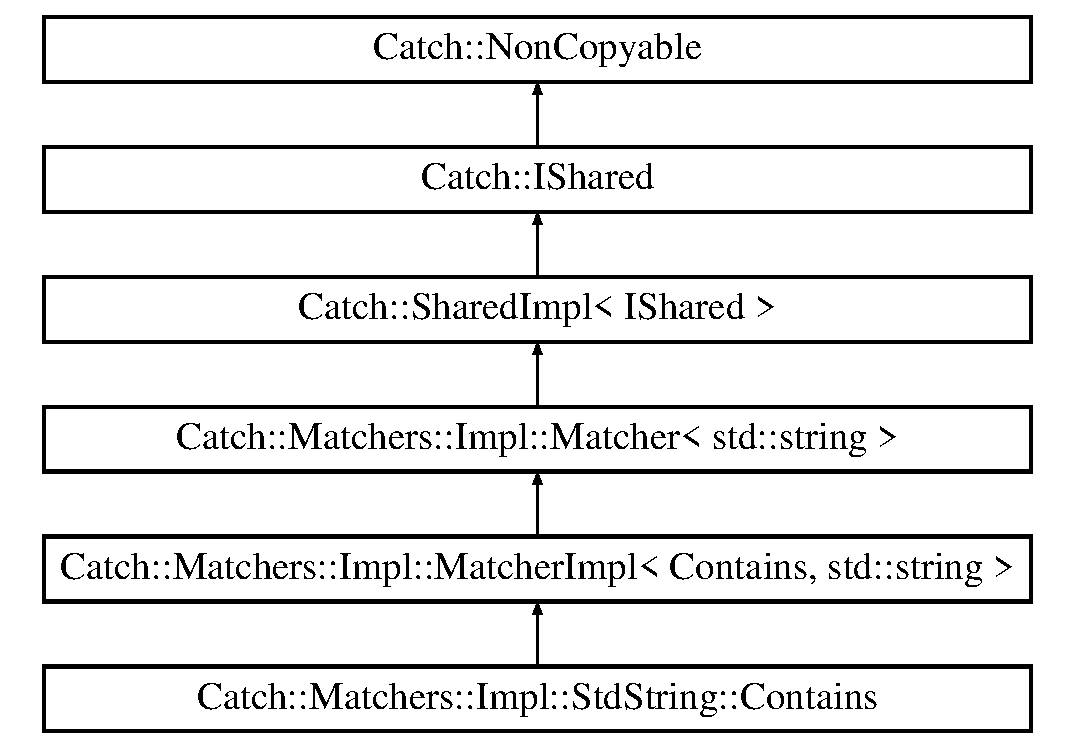
\includegraphics[height=6.000000cm]{struct_catch_1_1_matchers_1_1_impl_1_1_std_string_1_1_contains}
\end{center}
\end{figure}
\subsection*{Public Member Functions}
\begin{DoxyCompactItemize}
\item 
\mbox{\Hypertarget{struct_catch_1_1_matchers_1_1_impl_1_1_std_string_1_1_contains_a7a062d83bd3e3075929dbb55e1c24258}\label{struct_catch_1_1_matchers_1_1_impl_1_1_std_string_1_1_contains_a7a062d83bd3e3075929dbb55e1c24258}} 
{\bfseries Contains} (\textbf{ std\+::string} const \&substr, Case\+Sensitive\+::\+Choice case\+Sensitivity=Case\+Sensitive\+::\+Yes)
\item 
\mbox{\Hypertarget{struct_catch_1_1_matchers_1_1_impl_1_1_std_string_1_1_contains_ad6b1ef653dfcb3bab43c43be043dc4e8}\label{struct_catch_1_1_matchers_1_1_impl_1_1_std_string_1_1_contains_ad6b1ef653dfcb3bab43c43be043dc4e8}} 
{\bfseries Contains} (\hyperlink{struct_catch_1_1_matchers_1_1_impl_1_1_std_string_1_1_contains}{Contains} const \&other)
\item 
\mbox{\Hypertarget{struct_catch_1_1_matchers_1_1_impl_1_1_std_string_1_1_contains_a2248f3d0d1eb5cf5a1059c183b811a7c}\label{struct_catch_1_1_matchers_1_1_impl_1_1_std_string_1_1_contains_a2248f3d0d1eb5cf5a1059c183b811a7c}} 
virtual bool {\bfseries match} (\textbf{ std\+::string} const \&expr) const
\item 
\mbox{\Hypertarget{struct_catch_1_1_matchers_1_1_impl_1_1_std_string_1_1_contains_aed168ddff5bce9295aec5c7daca89849}\label{struct_catch_1_1_matchers_1_1_impl_1_1_std_string_1_1_contains_aed168ddff5bce9295aec5c7daca89849}} 
virtual \textbf{ std\+::string} {\bfseries to\+String} () const
\end{DoxyCompactItemize}
\subsection*{Public Attributes}
\begin{DoxyCompactItemize}
\item 
\mbox{\Hypertarget{struct_catch_1_1_matchers_1_1_impl_1_1_std_string_1_1_contains_a419a9ecaeaa417d4987982402e08b3eb}\label{struct_catch_1_1_matchers_1_1_impl_1_1_std_string_1_1_contains_a419a9ecaeaa417d4987982402e08b3eb}} 
\hyperlink{struct_catch_1_1_matchers_1_1_impl_1_1_std_string_1_1_cased_string}{Cased\+String} {\bfseries m\+\_\+data}
\end{DoxyCompactItemize}
\subsection*{Additional Inherited Members}


\subsection{Detailed Description}


Definition at line 1046 of file catch.\+hpp.



The documentation for this struct was generated from the following file\+:\begin{DoxyCompactItemize}
\item 
Tests/catch.\+hpp\end{DoxyCompactItemize}

\hypertarget{class_controller}{}\section{Controller Class Reference}
\label{class_controller}\index{Controller@{Controller}}


The \hyperlink{class_controller}{Controller} class It controls all the game and is the link between the view and the model.  




{\ttfamily \#include $<$controller.\+h$>$}

\subsection*{Public Member Functions}
\begin{DoxyCompactItemize}
\item 
\mbox{\Hypertarget{class_controller_a95c56822d667e94b031451729ce069a9}\label{class_controller_a95c56822d667e94b031451729ce069a9}} 
\hyperlink{class_controller_a95c56822d667e94b031451729ce069a9}{Controller} ()
\begin{DoxyCompactList}\small\item\em \hyperlink{class_controller}{Controller}, the constructor It creates an instance of the class from nothing. \end{DoxyCompactList}\item 
\mbox{\Hypertarget{class_controller_a0ab87934c4f7a266cfdb86e0f36bc1b5}\label{class_controller_a0ab87934c4f7a266cfdb86e0f36bc1b5}} 
\hyperlink{class_controller_a0ab87934c4f7a266cfdb86e0f36bc1b5}{$\sim$\+Controller} ()
\begin{DoxyCompactList}\small\item\em The destructor It deletes all the element from the class that need to be deleted. \end{DoxyCompactList}\item 
\hyperlink{class_controller}{Controller} \& \hyperlink{class_controller_ab237d20daccadca0d4bad9194d17c306}{operator=} (\hyperlink{class_controller}{Controller} \&o)
\begin{DoxyCompactList}\small\item\em operator = Assign the values of a controller to the current one. \end{DoxyCompactList}\item 
void \hyperlink{class_controller_a177d0d6cd7cdb7784ae9c506debfa2c6}{set\+Name} (\textbf{ std\+::string} name)
\begin{DoxyCompactList}\small\item\em set\+Name Sets the name of the player. \end{DoxyCompactList}\item 
void \hyperlink{class_controller_a7c1d65311fed834ed285040cd24cb320}{set\+Game} (\hyperlink{class_game}{Game} $\ast$g)
\begin{DoxyCompactList}\small\item\em set\+Game Sets the game in the controller. \end{DoxyCompactList}\item 
void \hyperlink{class_controller_ae83a66c83bfa72f2995aaa8ae1f23cfa}{first\+Play} (int i, int j)
\begin{DoxyCompactList}\small\item\em first\+Play Play for the first time. \end{DoxyCompactList}\item 
\textbf{ std\+::string} \hyperlink{class_controller_ac60aa220e5bf8cd0329b585c817bb5c4}{get\+Name} ()
\begin{DoxyCompactList}\small\item\em get\+Name Get the name of the user. \end{DoxyCompactList}\item 
int \hyperlink{class_controller_a108724342a6e4b06b0574c3a7d615bb2}{get\+Score} ()
\begin{DoxyCompactList}\small\item\em get\+Score Get the score of the user. \end{DoxyCompactList}\item 
bool \hyperlink{class_controller_a913c8ab636b486a26a4dd533d84e15b6}{add\+Score} (const \hyperlink{struct_board_type}{Board\+Type} \&board\+Type)
\begin{DoxyCompactList}\small\item\em add\+Score Add a score to the HoF. \end{DoxyCompactList}\item 
\hyperlink{class_game}{Game} $\ast$ \hyperlink{class_controller_aa6f9cab2dd64ec7f93e4834bf44ca4a7}{get\+Game} ()
\begin{DoxyCompactList}\small\item\em get\+Game Get the game. \end{DoxyCompactList}\item 
\hyperlink{class_hall_of_fame}{Hall\+Of\+Fame} \hyperlink{class_controller_abdad52832c8cd32d0f1e0c51442bda4c}{get\+H\+OF} ()
\begin{DoxyCompactList}\small\item\em get\+H\+OF Get the hall of fame. \end{DoxyCompactList}\item 
void \hyperlink{class_controller_a0f3954f7d90dba352953ce56491c5571}{play\+Once} (int i, int j, bool play)
\begin{DoxyCompactList}\small\item\em play\+Once Play a turn. \end{DoxyCompactList}\item 
int \hyperlink{class_controller_abaf42e3aabfc99cd4bc9c3395601e87f}{nb\+Bombs\+Default} (int i, int j)
\begin{DoxyCompactList}\small\item\em nb\+Bombs\+Default Calculte the number of bombs by default. \end{DoxyCompactList}\item 
bool \hyperlink{class_controller_a970af2439cfa0d315d769a4d92122928}{is\+Won} ()
\begin{DoxyCompactList}\small\item\em is\+Won Check if the player has won. \end{DoxyCompactList}\item 
bool \hyperlink{class_controller_a94cd37594f77fa357c9c6842884788d3}{is\+Over} ()
\begin{DoxyCompactList}\small\item\em is\+Over Check if the game of the user is over. \end{DoxyCompactList}\item 
\mbox{\Hypertarget{class_controller_aec60259dfc79f3100681447c9a0c3117}\label{class_controller_aec60259dfc79f3100681447c9a0c3117}} 
void \hyperlink{class_controller_aec60259dfc79f3100681447c9a0c3117}{activate\+Bonus} ()
\begin{DoxyCompactList}\small\item\em activate\+Bonus Use the bonus of the user. \end{DoxyCompactList}\item 
bool \hyperlink{class_controller_a6968f47298e55d9957bb330cf9cf957f}{is\+Bonus\+Used} ()
\begin{DoxyCompactList}\small\item\em is\+Bonus\+Used Check if the bonus is already used. \end{DoxyCompactList}\item 
void \hyperlink{class_controller_a6a06f685c0fdb19ceac20199db9916cd}{set\+Bonus\+Used} (bool used)
\begin{DoxyCompactList}\small\item\em set\+Bonus\+Used Set the bonus\+Used. \end{DoxyCompactList}\item 
void \hyperlink{class_controller_af9823d858e9ed334c8d20601f1e1fb02}{set\+Score} (int new\+Score)
\begin{DoxyCompactList}\small\item\em set\+Score Set the score of the user. \end{DoxyCompactList}\item 
int \hyperlink{class_controller_a1f5e158318b26e15a023391827617c04}{get\+Nb\+Click} ()
\begin{DoxyCompactList}\small\item\em get\+Nb\+Click Get the number of click of the user when he\textquotesingle{}s playing. \end{DoxyCompactList}\item 
\mbox{\Hypertarget{class_controller_a06c2739a07f098cfb843b0b4f6a3826f}\label{class_controller_a06c2739a07f098cfb843b0b4f6a3826f}} 
void \hyperlink{class_controller_a06c2739a07f098cfb843b0b4f6a3826f}{add\+Click} ()
\begin{DoxyCompactList}\small\item\em add\+Click Add a click on click count. \end{DoxyCompactList}\item 
\mbox{\Hypertarget{class_controller_a7b328695be686af4a9f7fe290781fbb0}\label{class_controller_a7b328695be686af4a9f7fe290781fbb0}} 
void \hyperlink{class_controller_a7b328695be686af4a9f7fe290781fbb0}{re\+Init} ()
\begin{DoxyCompactList}\small\item\em re\+Init Init the controller. \end{DoxyCompactList}\end{DoxyCompactItemize}


\subsection{Detailed Description}
The \hyperlink{class_controller}{Controller} class It controls all the game and is the link between the view and the model. 

Definition at line 12 of file controller.\+h.



\subsection{Member Function Documentation}
\mbox{\Hypertarget{class_controller_a913c8ab636b486a26a4dd533d84e15b6}\label{class_controller_a913c8ab636b486a26a4dd533d84e15b6}} 
\index{Controller@{Controller}!add\+Score@{add\+Score}}
\index{add\+Score@{add\+Score}!Controller@{Controller}}
\subsubsection{\texorpdfstring{add\+Score()}{addScore()}}
{\footnotesize\ttfamily bool Controller\+::add\+Score (\begin{DoxyParamCaption}\item[{const \hyperlink{struct_board_type}{Board\+Type} \&}]{board\+Type }\end{DoxyParamCaption})}



add\+Score Add a score to the HoF. 


\begin{DoxyParams}{Parameters}
{\em board\+Type} & The board\+Type of the last\+Game of the user. \\
\hline
\end{DoxyParams}
\begin{DoxyReturn}{Returns}
True if the user has a score that can be added and false if not. 
\end{DoxyReturn}


Definition at line 39 of file controller.\+cpp.

\mbox{\Hypertarget{class_controller_ae83a66c83bfa72f2995aaa8ae1f23cfa}\label{class_controller_ae83a66c83bfa72f2995aaa8ae1f23cfa}} 
\index{Controller@{Controller}!first\+Play@{first\+Play}}
\index{first\+Play@{first\+Play}!Controller@{Controller}}
\subsubsection{\texorpdfstring{first\+Play()}{firstPlay()}}
{\footnotesize\ttfamily void Controller\+::first\+Play (\begin{DoxyParamCaption}\item[{int}]{i,  }\item[{int}]{j }\end{DoxyParamCaption})}



first\+Play Play for the first time. 


\begin{DoxyParams}{Parameters}
{\em i} & The row of the board. \\
\hline
{\em j} & The column of the board. \\
\hline
\end{DoxyParams}


Definition at line 34 of file controller.\+cpp.

\mbox{\Hypertarget{class_controller_aa6f9cab2dd64ec7f93e4834bf44ca4a7}\label{class_controller_aa6f9cab2dd64ec7f93e4834bf44ca4a7}} 
\index{Controller@{Controller}!get\+Game@{get\+Game}}
\index{get\+Game@{get\+Game}!Controller@{Controller}}
\subsubsection{\texorpdfstring{get\+Game()}{getGame()}}
{\footnotesize\ttfamily \hyperlink{class_game}{Game} $\ast$ Controller\+::get\+Game (\begin{DoxyParamCaption}{ }\end{DoxyParamCaption})\hspace{0.3cm}{\ttfamily [inline]}}



get\+Game Get the game. 

\begin{DoxyReturn}{Returns}
The game of the controller. 
\end{DoxyReturn}


Definition at line 222 of file controller.\+h.

\mbox{\Hypertarget{class_controller_abdad52832c8cd32d0f1e0c51442bda4c}\label{class_controller_abdad52832c8cd32d0f1e0c51442bda4c}} 
\index{Controller@{Controller}!get\+H\+OF@{get\+H\+OF}}
\index{get\+H\+OF@{get\+H\+OF}!Controller@{Controller}}
\subsubsection{\texorpdfstring{get\+H\+O\+F()}{getHOF()}}
{\footnotesize\ttfamily \hyperlink{class_hall_of_fame}{Hall\+Of\+Fame} Controller\+::get\+H\+OF (\begin{DoxyParamCaption}{ }\end{DoxyParamCaption})\hspace{0.3cm}{\ttfamily [inline]}}



get\+H\+OF Get the hall of fame. 

\begin{DoxyReturn}{Returns}
The hall of fame of the game. 
\end{DoxyReturn}


Definition at line 226 of file controller.\+h.

\mbox{\Hypertarget{class_controller_ac60aa220e5bf8cd0329b585c817bb5c4}\label{class_controller_ac60aa220e5bf8cd0329b585c817bb5c4}} 
\index{Controller@{Controller}!get\+Name@{get\+Name}}
\index{get\+Name@{get\+Name}!Controller@{Controller}}
\subsubsection{\texorpdfstring{get\+Name()}{getName()}}
{\footnotesize\ttfamily \textbf{ std\+::string} Controller\+::get\+Name (\begin{DoxyParamCaption}{ }\end{DoxyParamCaption})\hspace{0.3cm}{\ttfamily [inline]}}



get\+Name Get the name of the user. 

\begin{DoxyReturn}{Returns}
The name of the user. 
\end{DoxyReturn}


Definition at line 206 of file controller.\+h.

\mbox{\Hypertarget{class_controller_a1f5e158318b26e15a023391827617c04}\label{class_controller_a1f5e158318b26e15a023391827617c04}} 
\index{Controller@{Controller}!get\+Nb\+Click@{get\+Nb\+Click}}
\index{get\+Nb\+Click@{get\+Nb\+Click}!Controller@{Controller}}
\subsubsection{\texorpdfstring{get\+Nb\+Click()}{getNbClick()}}
{\footnotesize\ttfamily int Controller\+::get\+Nb\+Click (\begin{DoxyParamCaption}{ }\end{DoxyParamCaption})\hspace{0.3cm}{\ttfamily [inline]}}



get\+Nb\+Click Get the number of click of the user when he\textquotesingle{}s playing. 

\begin{DoxyReturn}{Returns}
The number of click of the user when he\textquotesingle{}s playing. 
\end{DoxyReturn}


Definition at line 274 of file controller.\+h.

\mbox{\Hypertarget{class_controller_a108724342a6e4b06b0574c3a7d615bb2}\label{class_controller_a108724342a6e4b06b0574c3a7d615bb2}} 
\index{Controller@{Controller}!get\+Score@{get\+Score}}
\index{get\+Score@{get\+Score}!Controller@{Controller}}
\subsubsection{\texorpdfstring{get\+Score()}{getScore()}}
{\footnotesize\ttfamily int Controller\+::get\+Score (\begin{DoxyParamCaption}{ }\end{DoxyParamCaption})\hspace{0.3cm}{\ttfamily [inline]}}



get\+Score Get the score of the user. 

\begin{DoxyReturn}{Returns}
The score of the user. 
\end{DoxyReturn}


Definition at line 210 of file controller.\+h.

\mbox{\Hypertarget{class_controller_a6968f47298e55d9957bb330cf9cf957f}\label{class_controller_a6968f47298e55d9957bb330cf9cf957f}} 
\index{Controller@{Controller}!is\+Bonus\+Used@{is\+Bonus\+Used}}
\index{is\+Bonus\+Used@{is\+Bonus\+Used}!Controller@{Controller}}
\subsubsection{\texorpdfstring{is\+Bonus\+Used()}{isBonusUsed()}}
{\footnotesize\ttfamily bool Controller\+::is\+Bonus\+Used (\begin{DoxyParamCaption}{ }\end{DoxyParamCaption})\hspace{0.3cm}{\ttfamily [inline]}}



is\+Bonus\+Used Check if the bonus is already used. 

\begin{DoxyReturn}{Returns}
True if the user has already used his bonus and false if not. 
\end{DoxyReturn}


Definition at line 266 of file controller.\+h.

\mbox{\Hypertarget{class_controller_a94cd37594f77fa357c9c6842884788d3}\label{class_controller_a94cd37594f77fa357c9c6842884788d3}} 
\index{Controller@{Controller}!is\+Over@{is\+Over}}
\index{is\+Over@{is\+Over}!Controller@{Controller}}
\subsubsection{\texorpdfstring{is\+Over()}{isOver()}}
{\footnotesize\ttfamily bool Controller\+::is\+Over (\begin{DoxyParamCaption}{ }\end{DoxyParamCaption})\hspace{0.3cm}{\ttfamily [inline]}}



is\+Over Check if the game of the user is over. 

\begin{DoxyReturn}{Returns}
True if the game is over and false if not. 
\end{DoxyReturn}


Definition at line 255 of file controller.\+h.

\mbox{\Hypertarget{class_controller_a970af2439cfa0d315d769a4d92122928}\label{class_controller_a970af2439cfa0d315d769a4d92122928}} 
\index{Controller@{Controller}!is\+Won@{is\+Won}}
\index{is\+Won@{is\+Won}!Controller@{Controller}}
\subsubsection{\texorpdfstring{is\+Won()}{isWon()}}
{\footnotesize\ttfamily bool Controller\+::is\+Won (\begin{DoxyParamCaption}{ }\end{DoxyParamCaption})\hspace{0.3cm}{\ttfamily [inline]}}



is\+Won Check if the player has won. 

\begin{DoxyReturn}{Returns}
True if he won and false if not. 
\end{DoxyReturn}


Definition at line 251 of file controller.\+h.

\mbox{\Hypertarget{class_controller_abaf42e3aabfc99cd4bc9c3395601e87f}\label{class_controller_abaf42e3aabfc99cd4bc9c3395601e87f}} 
\index{Controller@{Controller}!nb\+Bombs\+Default@{nb\+Bombs\+Default}}
\index{nb\+Bombs\+Default@{nb\+Bombs\+Default}!Controller@{Controller}}
\subsubsection{\texorpdfstring{nb\+Bombs\+Default()}{nbBombsDefault()}}
{\footnotesize\ttfamily int Controller\+::nb\+Bombs\+Default (\begin{DoxyParamCaption}\item[{int}]{i,  }\item[{int}]{j }\end{DoxyParamCaption})\hspace{0.3cm}{\ttfamily [inline]}}



nb\+Bombs\+Default Calculte the number of bombs by default. 


\begin{DoxyParams}{Parameters}
{\em i} & The number of row. \\
\hline
{\em j} & The number of column. \\
\hline
\end{DoxyParams}
\begin{DoxyReturn}{Returns}
The number of bombs for this format. 
\end{DoxyReturn}


Definition at line 244 of file controller.\+h.

\mbox{\Hypertarget{class_controller_ab237d20daccadca0d4bad9194d17c306}\label{class_controller_ab237d20daccadca0d4bad9194d17c306}} 
\index{Controller@{Controller}!operator=@{operator=}}
\index{operator=@{operator=}!Controller@{Controller}}
\subsubsection{\texorpdfstring{operator=()}{operator=()}}
{\footnotesize\ttfamily \hyperlink{class_controller}{Controller} \& Controller\+::operator= (\begin{DoxyParamCaption}\item[{\hyperlink{class_controller}{Controller} \&}]{o }\end{DoxyParamCaption})\hspace{0.3cm}{\ttfamily [inline]}}



operator = Assign the values of a controller to the current one. 


\begin{DoxyParams}{Parameters}
{\em o} & the controller that will give its value. \\
\hline
\end{DoxyParams}
\begin{DoxyReturn}{Returns}
the newly formed controller. 
\end{DoxyReturn}


Definition at line 230 of file controller.\+h.

\mbox{\Hypertarget{class_controller_a0f3954f7d90dba352953ce56491c5571}\label{class_controller_a0f3954f7d90dba352953ce56491c5571}} 
\index{Controller@{Controller}!play\+Once@{play\+Once}}
\index{play\+Once@{play\+Once}!Controller@{Controller}}
\subsubsection{\texorpdfstring{play\+Once()}{playOnce()}}
{\footnotesize\ttfamily void Controller\+::play\+Once (\begin{DoxyParamCaption}\item[{int}]{i,  }\item[{int}]{j,  }\item[{bool}]{play }\end{DoxyParamCaption})}



play\+Once Play a turn. 


\begin{DoxyParams}{Parameters}
{\em i} & The row of board. \\
\hline
{\em j} & The column of the board. \\
\hline
{\em play} & True if the user wants to unveil a case and false if he just wants to flag a case. \\
\hline
\end{DoxyParams}


Definition at line 50 of file controller.\+cpp.

\mbox{\Hypertarget{class_controller_a6a06f685c0fdb19ceac20199db9916cd}\label{class_controller_a6a06f685c0fdb19ceac20199db9916cd}} 
\index{Controller@{Controller}!set\+Bonus\+Used@{set\+Bonus\+Used}}
\index{set\+Bonus\+Used@{set\+Bonus\+Used}!Controller@{Controller}}
\subsubsection{\texorpdfstring{set\+Bonus\+Used()}{setBonusUsed()}}
{\footnotesize\ttfamily void Controller\+::set\+Bonus\+Used (\begin{DoxyParamCaption}\item[{bool}]{used }\end{DoxyParamCaption})\hspace{0.3cm}{\ttfamily [inline]}}



set\+Bonus\+Used Set the bonus\+Used. 


\begin{DoxyParams}{Parameters}
{\em used} & The new value of bonus\+Used. \\
\hline
\end{DoxyParams}


Definition at line 270 of file controller.\+h.

\mbox{\Hypertarget{class_controller_a7c1d65311fed834ed285040cd24cb320}\label{class_controller_a7c1d65311fed834ed285040cd24cb320}} 
\index{Controller@{Controller}!set\+Game@{set\+Game}}
\index{set\+Game@{set\+Game}!Controller@{Controller}}
\subsubsection{\texorpdfstring{set\+Game()}{setGame()}}
{\footnotesize\ttfamily void Controller\+::set\+Game (\begin{DoxyParamCaption}\item[{\hyperlink{class_game}{Game} $\ast$}]{g }\end{DoxyParamCaption})\hspace{0.3cm}{\ttfamily [inline]}}



set\+Game Sets the game in the controller. 


\begin{DoxyParams}{Parameters}
{\em g} & The game to set. \\
\hline
\end{DoxyParams}


Definition at line 240 of file controller.\+h.

\mbox{\Hypertarget{class_controller_a177d0d6cd7cdb7784ae9c506debfa2c6}\label{class_controller_a177d0d6cd7cdb7784ae9c506debfa2c6}} 
\index{Controller@{Controller}!set\+Name@{set\+Name}}
\index{set\+Name@{set\+Name}!Controller@{Controller}}
\subsubsection{\texorpdfstring{set\+Name()}{setName()}}
{\footnotesize\ttfamily void Controller\+::set\+Name (\begin{DoxyParamCaption}\item[{\textbf{ std\+::string}}]{name }\end{DoxyParamCaption})\hspace{0.3cm}{\ttfamily [inline]}}



set\+Name Sets the name of the player. 


\begin{DoxyParams}{Parameters}
{\em name} & the name of the player. \\
\hline
\end{DoxyParams}


Definition at line 218 of file controller.\+h.

\mbox{\Hypertarget{class_controller_af9823d858e9ed334c8d20601f1e1fb02}\label{class_controller_af9823d858e9ed334c8d20601f1e1fb02}} 
\index{Controller@{Controller}!set\+Score@{set\+Score}}
\index{set\+Score@{set\+Score}!Controller@{Controller}}
\subsubsection{\texorpdfstring{set\+Score()}{setScore()}}
{\footnotesize\ttfamily void Controller\+::set\+Score (\begin{DoxyParamCaption}\item[{int}]{new\+Score }\end{DoxyParamCaption})\hspace{0.3cm}{\ttfamily [inline]}}



set\+Score Set the score of the user. 


\begin{DoxyParams}{Parameters}
{\em new\+Score} & The new score of the user. \\
\hline
\end{DoxyParams}


Definition at line 214 of file controller.\+h.



The documentation for this class was generated from the following files\+:\begin{DoxyCompactItemize}
\item 
Application/controller.\+h\item 
Application/controller.\+cpp\end{DoxyCompactItemize}

\hypertarget{struct_coordinates}{}\section{Coordinates Struct Reference}
\label{struct_coordinates}\index{Coordinates@{Coordinates}}


\hyperlink{struct_coordinates}{Coordinates}, the coordinates of a case. The coordinates of the case is composed of a x-\/axis value, row, and a y-\/axis value, column Theses are used to localize the cases in the board.  




{\ttfamily \#include $<$structure.\+h$>$}

\subsection*{Public Member Functions}
\begin{DoxyCompactItemize}
\item 
\hyperlink{struct_coordinates}{Coordinates} \& \hyperlink{struct_coordinates_a150b9f9ce9574f29bec14407021e7292}{operator=} (const \hyperlink{struct_coordinates}{Coordinates} \&a)
\begin{DoxyCompactList}\small\item\em operator = Assigns the value of a \hyperlink{struct_coordinates}{Coordinates} to a new one. \end{DoxyCompactList}\end{DoxyCompactItemize}
\subsection*{Public Attributes}
\begin{DoxyCompactItemize}
\item 
\mbox{\Hypertarget{struct_coordinates_aa3e522bbc0eab18fe35a7b17186df35e}\label{struct_coordinates_aa3e522bbc0eab18fe35a7b17186df35e}} 
int \hyperlink{struct_coordinates_aa3e522bbc0eab18fe35a7b17186df35e}{row}
\begin{DoxyCompactList}\small\item\em row the row of a case \end{DoxyCompactList}\item 
\mbox{\Hypertarget{struct_coordinates_a4d1e2bdd28dfd0a047e4b1f9fcb04a31}\label{struct_coordinates_a4d1e2bdd28dfd0a047e4b1f9fcb04a31}} 
int \hyperlink{struct_coordinates_a4d1e2bdd28dfd0a047e4b1f9fcb04a31}{col}
\begin{DoxyCompactList}\small\item\em col the column of a case \end{DoxyCompactList}\end{DoxyCompactItemize}


\subsection{Detailed Description}
\hyperlink{struct_coordinates}{Coordinates}, the coordinates of a case. The coordinates of the case is composed of a x-\/axis value, row, and a y-\/axis value, column Theses are used to localize the cases in the board. 

Definition at line 90 of file structure.\+h.



\subsection{Member Function Documentation}
\mbox{\Hypertarget{struct_coordinates_a150b9f9ce9574f29bec14407021e7292}\label{struct_coordinates_a150b9f9ce9574f29bec14407021e7292}} 
\index{Coordinates@{Coordinates}!operator=@{operator=}}
\index{operator=@{operator=}!Coordinates@{Coordinates}}
\subsubsection{\texorpdfstring{operator=()}{operator=()}}
{\footnotesize\ttfamily \hyperlink{struct_coordinates}{Coordinates}\& Coordinates\+::operator= (\begin{DoxyParamCaption}\item[{const \hyperlink{struct_coordinates}{Coordinates} \&}]{a }\end{DoxyParamCaption})\hspace{0.3cm}{\ttfamily [inline]}}



operator = Assigns the value of a \hyperlink{struct_coordinates}{Coordinates} to a new one. 


\begin{DoxyParams}{Parameters}
{\em a} & the \hyperlink{struct_coordinates}{Coordinates} we take the value from. \\
\hline
\end{DoxyParams}
\begin{DoxyReturn}{Returns}
a new \hyperlink{struct_coordinates}{Coordinates}, that has the same value as the other one. 
\end{DoxyReturn}


Definition at line 110 of file structure.\+h.



The documentation for this struct was generated from the following file\+:\begin{DoxyCompactItemize}
\item 
Application/structure.\+h\end{DoxyCompactItemize}

\hypertarget{struct_catch_1_1_copyable_stream}{}\section{Catch\+:\+:Copyable\+Stream Struct Reference}
\label{struct_catch_1_1_copyable_stream}\index{Catch\+::\+Copyable\+Stream@{Catch\+::\+Copyable\+Stream}}
\subsection*{Public Member Functions}
\begin{DoxyCompactItemize}
\item 
\mbox{\Hypertarget{struct_catch_1_1_copyable_stream_a0e72dc16240653f52c17106f4bf34da8}\label{struct_catch_1_1_copyable_stream_a0e72dc16240653f52c17106f4bf34da8}} 
{\bfseries Copyable\+Stream} (\hyperlink{struct_catch_1_1_copyable_stream}{Copyable\+Stream} const \&other)
\item 
\mbox{\Hypertarget{struct_catch_1_1_copyable_stream_a1760fa29b38011c5845171260bec0966}\label{struct_catch_1_1_copyable_stream_a1760fa29b38011c5845171260bec0966}} 
\hyperlink{struct_catch_1_1_copyable_stream}{Copyable\+Stream} \& {\bfseries operator=} (\hyperlink{struct_catch_1_1_copyable_stream}{Copyable\+Stream} const \&other)
\end{DoxyCompactItemize}
\subsection*{Public Attributes}
\begin{DoxyCompactItemize}
\item 
\mbox{\Hypertarget{struct_catch_1_1_copyable_stream_ae123fb4d673e7d7a13a3c5f6bc5d426c}\label{struct_catch_1_1_copyable_stream_ae123fb4d673e7d7a13a3c5f6bc5d426c}} 
\textbf{ std\+::ostringstream} {\bfseries oss}
\end{DoxyCompactItemize}


\subsection{Detailed Description}


Definition at line 1169 of file catch.\+hpp.



The documentation for this struct was generated from the following file\+:\begin{DoxyCompactItemize}
\item 
Tests/catch.\+hpp\end{DoxyCompactItemize}

\hypertarget{struct_catch_1_1_counts}{}\section{Catch\+:\+:Counts Struct Reference}
\label{struct_catch_1_1_counts}\index{Catch\+::\+Counts@{Catch\+::\+Counts}}
\subsection*{Public Member Functions}
\begin{DoxyCompactItemize}
\item 
\mbox{\Hypertarget{struct_catch_1_1_counts_aaa10666f559057e3e860d2a5a6fae4c4}\label{struct_catch_1_1_counts_aaa10666f559057e3e860d2a5a6fae4c4}} 
\hyperlink{struct_catch_1_1_counts}{Counts} {\bfseries operator-\/} (\hyperlink{struct_catch_1_1_counts}{Counts} const \&other) const
\item 
\mbox{\Hypertarget{struct_catch_1_1_counts_a322a89475cd2cc039140ef371e973677}\label{struct_catch_1_1_counts_a322a89475cd2cc039140ef371e973677}} 
\hyperlink{struct_catch_1_1_counts}{Counts} \& {\bfseries operator+=} (\hyperlink{struct_catch_1_1_counts}{Counts} const \&other)
\item 
\mbox{\Hypertarget{struct_catch_1_1_counts_a94f969c09cf52d1339c085c9603cd1d3}\label{struct_catch_1_1_counts_a94f969c09cf52d1339c085c9603cd1d3}} 
\textbf{ std\+::size\+\_\+t} {\bfseries total} () const
\item 
\mbox{\Hypertarget{struct_catch_1_1_counts_a84999490e0ecaa3de5e121bf48eda1b3}\label{struct_catch_1_1_counts_a84999490e0ecaa3de5e121bf48eda1b3}} 
bool {\bfseries all\+Passed} () const
\item 
\mbox{\Hypertarget{struct_catch_1_1_counts_a33bd996e016030155b99fe1c51c08991}\label{struct_catch_1_1_counts_a33bd996e016030155b99fe1c51c08991}} 
bool {\bfseries all\+Ok} () const
\end{DoxyCompactItemize}
\subsection*{Public Attributes}
\begin{DoxyCompactItemize}
\item 
\mbox{\Hypertarget{struct_catch_1_1_counts_ad28daaf3de28006400208b6dd0c631e6}\label{struct_catch_1_1_counts_ad28daaf3de28006400208b6dd0c631e6}} 
\textbf{ std\+::size\+\_\+t} {\bfseries passed}
\item 
\mbox{\Hypertarget{struct_catch_1_1_counts_a19982a3817a3bc2c07f0290e71f497a3}\label{struct_catch_1_1_counts_a19982a3817a3bc2c07f0290e71f497a3}} 
\textbf{ std\+::size\+\_\+t} {\bfseries failed}
\item 
\mbox{\Hypertarget{struct_catch_1_1_counts_ac090973a2ff51394cd452718e75c073e}\label{struct_catch_1_1_counts_ac090973a2ff51394cd452718e75c073e}} 
\textbf{ std\+::size\+\_\+t} {\bfseries failed\+But\+Ok}
\end{DoxyCompactItemize}


\subsection{Detailed Description}


Definition at line 2146 of file catch.\+hpp.



The documentation for this struct was generated from the following file\+:\begin{DoxyCompactItemize}
\item 
Tests/catch.\+hpp\end{DoxyCompactItemize}

\hypertarget{struct_dimension}{}\section{Dimension Struct Reference}
\label{struct_dimension}\index{Dimension@{Dimension}}


\hyperlink{struct_dimension}{Dimension}, the dimension of the board. A dimension is composed of an height and a width.  




{\ttfamily \#include $<$structure.\+h$>$}

\subsection*{Public Member Functions}
\begin{DoxyCompactItemize}
\item 
\hyperlink{struct_dimension}{Dimension} \& \hyperlink{struct_dimension_acbce569721e053b72d6ed134ed649fe4}{operator=} (const \hyperlink{struct_dimension}{Dimension} \&a)
\begin{DoxyCompactList}\small\item\em operator = Assigns the value of a \hyperlink{struct_dimension}{Dimension} to a new one. \end{DoxyCompactList}\item 
bool \hyperlink{struct_dimension_a193e00a30205877faa6eb2978e11894f}{operator$<$} (const \hyperlink{struct_dimension}{Dimension} \&r) const
\begin{DoxyCompactList}\small\item\em operator $<$ Verifies if a \hyperlink{struct_dimension}{Dimension} is smaller than another. \end{DoxyCompactList}\item 
bool \hyperlink{struct_dimension_a31342c295eeff5e9fc89e47656192c5d}{operator$>$} (const \hyperlink{struct_dimension}{Dimension} \&r) const
\begin{DoxyCompactList}\small\item\em operator $>$ Verifies if a \hyperlink{struct_dimension}{Dimension} is greater than another. \end{DoxyCompactList}\item 
bool \hyperlink{struct_dimension_aa50ef143b3130d4810950788a580b342}{operator==} (const \hyperlink{struct_dimension}{Dimension} \&dim)
\begin{DoxyCompactList}\small\item\em operator == Verifies if two Dimensions have the same values. \end{DoxyCompactList}\end{DoxyCompactItemize}
\subsection*{Public Attributes}
\begin{DoxyCompactItemize}
\item 
\mbox{\Hypertarget{struct_dimension_ae6458fe2808cda65f04a61d532bd45df}\label{struct_dimension_ae6458fe2808cda65f04a61d532bd45df}} 
int \hyperlink{struct_dimension_ae6458fe2808cda65f04a61d532bd45df}{height}
\begin{DoxyCompactList}\small\item\em height the height of the board. \end{DoxyCompactList}\item 
\mbox{\Hypertarget{struct_dimension_a9ccec48bbada6d1b8aaa9a1e5fc60fcd}\label{struct_dimension_a9ccec48bbada6d1b8aaa9a1e5fc60fcd}} 
int \hyperlink{struct_dimension_a9ccec48bbada6d1b8aaa9a1e5fc60fcd}{width}
\begin{DoxyCompactList}\small\item\em width the width of the board. \end{DoxyCompactList}\end{DoxyCompactItemize}


\subsection{Detailed Description}
\hyperlink{struct_dimension}{Dimension}, the dimension of the board. A dimension is composed of an height and a width. 

Definition at line 8 of file structure.\+h.



\subsection{Member Function Documentation}
\mbox{\Hypertarget{struct_dimension_a193e00a30205877faa6eb2978e11894f}\label{struct_dimension_a193e00a30205877faa6eb2978e11894f}} 
\index{Dimension@{Dimension}!operator$<$@{operator$<$}}
\index{operator$<$@{operator$<$}!Dimension@{Dimension}}
\subsubsection{\texorpdfstring{operator$<$()}{operator<()}}
{\footnotesize\ttfamily bool Dimension\+::operator$<$ (\begin{DoxyParamCaption}\item[{const \hyperlink{struct_dimension}{Dimension} \&}]{r }\end{DoxyParamCaption}) const\hspace{0.3cm}{\ttfamily [inline]}}



operator $<$ Verifies if a \hyperlink{struct_dimension}{Dimension} is smaller than another. 


\begin{DoxyParams}{Parameters}
{\em a} & the \hyperlink{struct_dimension}{Dimension} the current \hyperlink{struct_dimension}{Dimension} is compared to. \\
\hline
\end{DoxyParams}
\begin{DoxyReturn}{Returns}
true if the \hyperlink{struct_dimension}{Dimension} is smaller, false otherwise. 
\end{DoxyReturn}


Definition at line 40 of file structure.\+h.

\mbox{\Hypertarget{struct_dimension_acbce569721e053b72d6ed134ed649fe4}\label{struct_dimension_acbce569721e053b72d6ed134ed649fe4}} 
\index{Dimension@{Dimension}!operator=@{operator=}}
\index{operator=@{operator=}!Dimension@{Dimension}}
\subsubsection{\texorpdfstring{operator=()}{operator=()}}
{\footnotesize\ttfamily \hyperlink{struct_dimension}{Dimension}\& Dimension\+::operator= (\begin{DoxyParamCaption}\item[{const \hyperlink{struct_dimension}{Dimension} \&}]{a }\end{DoxyParamCaption})\hspace{0.3cm}{\ttfamily [inline]}}



operator = Assigns the value of a \hyperlink{struct_dimension}{Dimension} to a new one. 


\begin{DoxyParams}{Parameters}
{\em a} & the \hyperlink{struct_dimension}{Dimension} we take the value from. \\
\hline
\end{DoxyParams}
\begin{DoxyReturn}{Returns}
a new \hyperlink{struct_dimension}{Dimension}, that has the same value as the other one. 
\end{DoxyReturn}


Definition at line 28 of file structure.\+h.

\mbox{\Hypertarget{struct_dimension_aa50ef143b3130d4810950788a580b342}\label{struct_dimension_aa50ef143b3130d4810950788a580b342}} 
\index{Dimension@{Dimension}!operator==@{operator==}}
\index{operator==@{operator==}!Dimension@{Dimension}}
\subsubsection{\texorpdfstring{operator==()}{operator==()}}
{\footnotesize\ttfamily bool Dimension\+::operator== (\begin{DoxyParamCaption}\item[{const \hyperlink{struct_dimension}{Dimension} \&}]{dim }\end{DoxyParamCaption})\hspace{0.3cm}{\ttfamily [inline]}}



operator == Verifies if two Dimensions have the same values. 


\begin{DoxyParams}{Parameters}
{\em a} & the \hyperlink{struct_dimension}{Dimension} the current \hyperlink{struct_dimension}{Dimension} is compared to. \\
\hline
\end{DoxyParams}
\begin{DoxyReturn}{Returns}
true if the \hyperlink{struct_dimension}{Dimension} are equals, false otherwise. 
\end{DoxyReturn}


Definition at line 78 of file structure.\+h.

\mbox{\Hypertarget{struct_dimension_a31342c295eeff5e9fc89e47656192c5d}\label{struct_dimension_a31342c295eeff5e9fc89e47656192c5d}} 
\index{Dimension@{Dimension}!operator$>$@{operator$>$}}
\index{operator$>$@{operator$>$}!Dimension@{Dimension}}
\subsubsection{\texorpdfstring{operator$>$()}{operator>()}}
{\footnotesize\ttfamily bool Dimension\+::operator$>$ (\begin{DoxyParamCaption}\item[{const \hyperlink{struct_dimension}{Dimension} \&}]{r }\end{DoxyParamCaption}) const\hspace{0.3cm}{\ttfamily [inline]}}



operator $>$ Verifies if a \hyperlink{struct_dimension}{Dimension} is greater than another. 


\begin{DoxyParams}{Parameters}
{\em a} & the \hyperlink{struct_dimension}{Dimension} the current \hyperlink{struct_dimension}{Dimension} is compared to. \\
\hline
\end{DoxyParams}
\begin{DoxyReturn}{Returns}
true if the \hyperlink{struct_dimension}{Dimension} is greater, false otherwise. 
\end{DoxyReturn}


Definition at line 59 of file structure.\+h.



The documentation for this struct was generated from the following file\+:\begin{DoxyCompactItemize}
\item 
Application/structure.\+h\end{DoxyCompactItemize}

\hypertarget{struct_catch_1_1_matchers_1_1_impl_1_1_std_string_1_1_ends_with}{}\section{Catch\+:\+:Matchers\+:\+:Impl\+:\+:Std\+String\+:\+:Ends\+With Struct Reference}
\label{struct_catch_1_1_matchers_1_1_impl_1_1_std_string_1_1_ends_with}\index{Catch\+::\+Matchers\+::\+Impl\+::\+Std\+String\+::\+Ends\+With@{Catch\+::\+Matchers\+::\+Impl\+::\+Std\+String\+::\+Ends\+With}}
Inheritance diagram for Catch\+:\+:Matchers\+:\+:Impl\+:\+:Std\+String\+:\+:Ends\+With\+:\begin{figure}[H]
\begin{center}
\leavevmode
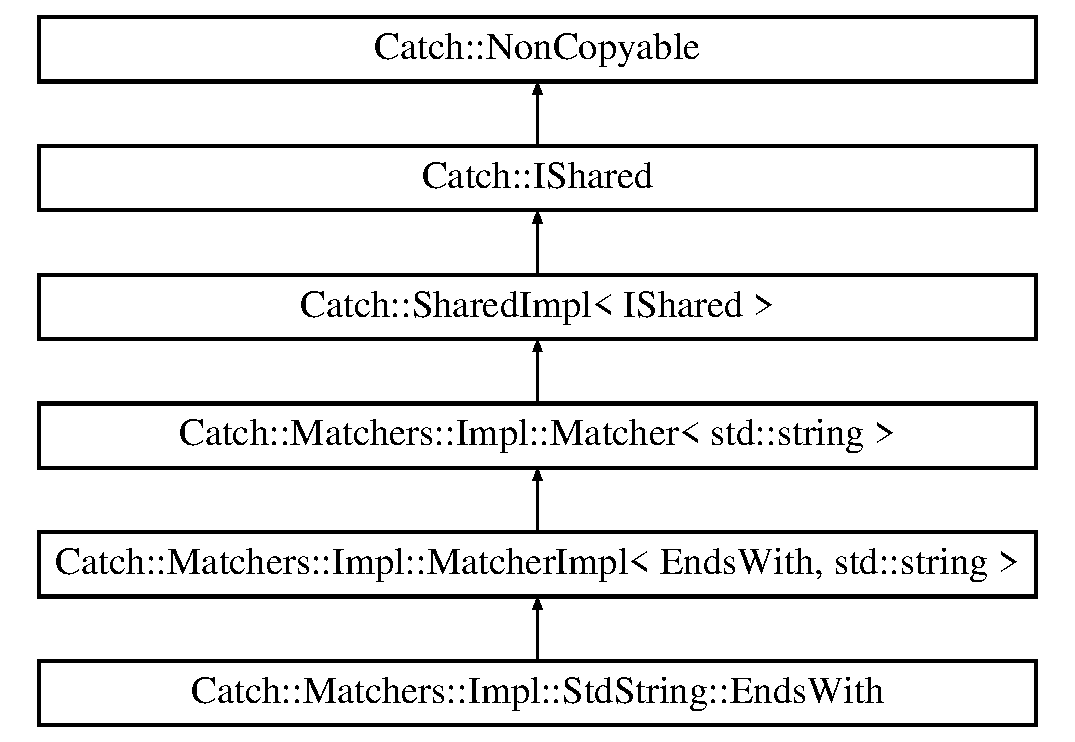
\includegraphics[height=6.000000cm]{struct_catch_1_1_matchers_1_1_impl_1_1_std_string_1_1_ends_with}
\end{center}
\end{figure}
\subsection*{Public Member Functions}
\begin{DoxyCompactItemize}
\item 
\mbox{\Hypertarget{struct_catch_1_1_matchers_1_1_impl_1_1_std_string_1_1_ends_with_ae90c02ff06c9dd5e62218b2b521e8cab}\label{struct_catch_1_1_matchers_1_1_impl_1_1_std_string_1_1_ends_with_ae90c02ff06c9dd5e62218b2b521e8cab}} 
{\bfseries Ends\+With} (\textbf{ std\+::string} const \&substr, Case\+Sensitive\+::\+Choice case\+Sensitivity=Case\+Sensitive\+::\+Yes)
\item 
\mbox{\Hypertarget{struct_catch_1_1_matchers_1_1_impl_1_1_std_string_1_1_ends_with_a9321aac07fb17613a7993e99003b3be2}\label{struct_catch_1_1_matchers_1_1_impl_1_1_std_string_1_1_ends_with_a9321aac07fb17613a7993e99003b3be2}} 
{\bfseries Ends\+With} (\hyperlink{struct_catch_1_1_matchers_1_1_impl_1_1_std_string_1_1_ends_with}{Ends\+With} const \&other)
\item 
\mbox{\Hypertarget{struct_catch_1_1_matchers_1_1_impl_1_1_std_string_1_1_ends_with_aff66fb5af2d4f6161627cb20899b2c1b}\label{struct_catch_1_1_matchers_1_1_impl_1_1_std_string_1_1_ends_with_aff66fb5af2d4f6161627cb20899b2c1b}} 
virtual bool {\bfseries match} (\textbf{ std\+::string} const \&expr) const
\item 
\mbox{\Hypertarget{struct_catch_1_1_matchers_1_1_impl_1_1_std_string_1_1_ends_with_a2a4675e3d2369d587af36f051fb7964f}\label{struct_catch_1_1_matchers_1_1_impl_1_1_std_string_1_1_ends_with_a2a4675e3d2369d587af36f051fb7964f}} 
virtual \textbf{ std\+::string} {\bfseries to\+String} () const
\end{DoxyCompactItemize}
\subsection*{Public Attributes}
\begin{DoxyCompactItemize}
\item 
\mbox{\Hypertarget{struct_catch_1_1_matchers_1_1_impl_1_1_std_string_1_1_ends_with_a344d8433f3ba3e0de301ab16ed6dd746}\label{struct_catch_1_1_matchers_1_1_impl_1_1_std_string_1_1_ends_with_a344d8433f3ba3e0de301ab16ed6dd746}} 
\hyperlink{struct_catch_1_1_matchers_1_1_impl_1_1_std_string_1_1_cased_string}{Cased\+String} {\bfseries m\+\_\+data}
\end{DoxyCompactItemize}
\subsection*{Additional Inherited Members}


\subsection{Detailed Description}


Definition at line 1081 of file catch.\+hpp.



The documentation for this struct was generated from the following file\+:\begin{DoxyCompactItemize}
\item 
Tests/catch.\+hpp\end{DoxyCompactItemize}

\hypertarget{struct_catch_1_1_matchers_1_1_impl_1_1_std_string_1_1_equals}{}\section{Catch\+:\+:Matchers\+:\+:Impl\+:\+:Std\+String\+:\+:Equals Struct Reference}
\label{struct_catch_1_1_matchers_1_1_impl_1_1_std_string_1_1_equals}\index{Catch\+::\+Matchers\+::\+Impl\+::\+Std\+String\+::\+Equals@{Catch\+::\+Matchers\+::\+Impl\+::\+Std\+String\+::\+Equals}}
Inheritance diagram for Catch\+:\+:Matchers\+:\+:Impl\+:\+:Std\+String\+:\+:Equals\+:\begin{figure}[H]
\begin{center}
\leavevmode
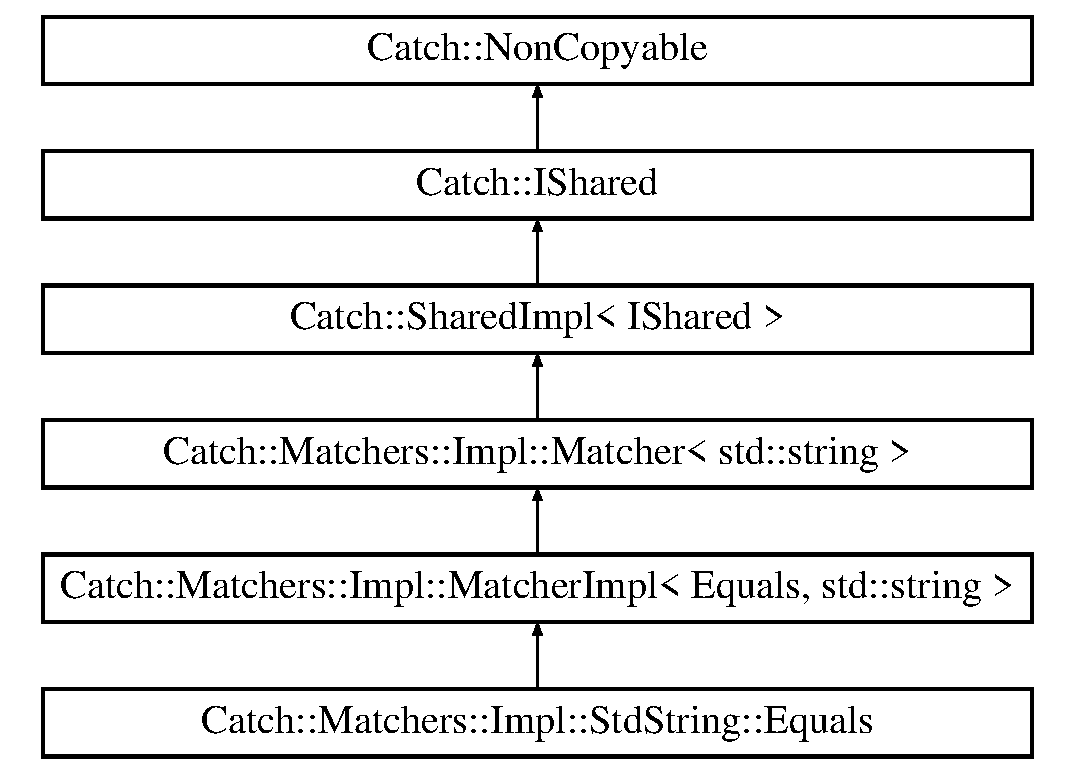
\includegraphics[height=6.000000cm]{struct_catch_1_1_matchers_1_1_impl_1_1_std_string_1_1_equals}
\end{center}
\end{figure}
\subsection*{Public Member Functions}
\begin{DoxyCompactItemize}
\item 
\mbox{\Hypertarget{struct_catch_1_1_matchers_1_1_impl_1_1_std_string_1_1_equals_a5921d5ed75320fb64a678e3f1292a464}\label{struct_catch_1_1_matchers_1_1_impl_1_1_std_string_1_1_equals_a5921d5ed75320fb64a678e3f1292a464}} 
{\bfseries Equals} (\textbf{ std\+::string} const \&str, Case\+Sensitive\+::\+Choice case\+Sensitivity=Case\+Sensitive\+::\+Yes)
\item 
\mbox{\Hypertarget{struct_catch_1_1_matchers_1_1_impl_1_1_std_string_1_1_equals_acaa97de06aedf363ae803d65a975f5e4}\label{struct_catch_1_1_matchers_1_1_impl_1_1_std_string_1_1_equals_acaa97de06aedf363ae803d65a975f5e4}} 
{\bfseries Equals} (\hyperlink{struct_catch_1_1_matchers_1_1_impl_1_1_std_string_1_1_equals}{Equals} const \&other)
\item 
\mbox{\Hypertarget{struct_catch_1_1_matchers_1_1_impl_1_1_std_string_1_1_equals_abf0a94b4e66dbd586268d9983f867e68}\label{struct_catch_1_1_matchers_1_1_impl_1_1_std_string_1_1_equals_abf0a94b4e66dbd586268d9983f867e68}} 
virtual bool {\bfseries match} (\textbf{ std\+::string} const \&expr) const
\item 
\mbox{\Hypertarget{struct_catch_1_1_matchers_1_1_impl_1_1_std_string_1_1_equals_ab0d73961b95d9836d77b9e2e94c3790b}\label{struct_catch_1_1_matchers_1_1_impl_1_1_std_string_1_1_equals_ab0d73961b95d9836d77b9e2e94c3790b}} 
virtual \textbf{ std\+::string} {\bfseries to\+String} () const
\end{DoxyCompactItemize}
\subsection*{Public Attributes}
\begin{DoxyCompactItemize}
\item 
\mbox{\Hypertarget{struct_catch_1_1_matchers_1_1_impl_1_1_std_string_1_1_equals_ae09964b7ba291ce574b514a2ee3eddb0}\label{struct_catch_1_1_matchers_1_1_impl_1_1_std_string_1_1_equals_ae09964b7ba291ce574b514a2ee3eddb0}} 
\hyperlink{struct_catch_1_1_matchers_1_1_impl_1_1_std_string_1_1_cased_string}{Cased\+String} {\bfseries m\+\_\+data}
\end{DoxyCompactItemize}
\subsection*{Additional Inherited Members}


\subsection{Detailed Description}


Definition at line 1028 of file catch.\+hpp.



The documentation for this struct was generated from the following file\+:\begin{DoxyCompactItemize}
\item 
Tests/catch.\+hpp\end{DoxyCompactItemize}

\hypertarget{class_catch_1_1_internal_1_1_evaluator}{}\section{Catch\+:\+:Internal\+:\+:Evaluator$<$ T1, T2, Op $>$ Class Template Reference}
\label{class_catch_1_1_internal_1_1_evaluator}\index{Catch\+::\+Internal\+::\+Evaluator$<$ T1, T2, Op $>$@{Catch\+::\+Internal\+::\+Evaluator$<$ T1, T2, Op $>$}}


\subsection{Detailed Description}
\subsubsection*{template$<$typename T1, typename T2, Operator Op$>$\newline
class Catch\+::\+Internal\+::\+Evaluator$<$ T1, T2, Op $>$}



Definition at line 1285 of file catch.\+hpp.



The documentation for this class was generated from the following file\+:\begin{DoxyCompactItemize}
\item 
Tests/catch.\+hpp\end{DoxyCompactItemize}

\hypertarget{struct_catch_1_1_internal_1_1_evaluator_3_01_t1_00_01_t2_00_01_is_equal_to_01_4}{}\section{Catch\+:\+:Internal\+:\+:Evaluator$<$ T1, T2, Is\+Equal\+To $>$ Struct Template Reference}
\label{struct_catch_1_1_internal_1_1_evaluator_3_01_t1_00_01_t2_00_01_is_equal_to_01_4}\index{Catch\+::\+Internal\+::\+Evaluator$<$ T1, T2, Is\+Equal\+To $>$@{Catch\+::\+Internal\+::\+Evaluator$<$ T1, T2, Is\+Equal\+To $>$}}
\subsection*{Static Public Member Functions}
\begin{DoxyCompactItemize}
\item 
\mbox{\Hypertarget{struct_catch_1_1_internal_1_1_evaluator_3_01_t1_00_01_t2_00_01_is_equal_to_01_4_a166b2b7849247397e63fb2940481b217}\label{struct_catch_1_1_internal_1_1_evaluator_3_01_t1_00_01_t2_00_01_is_equal_to_01_4_a166b2b7849247397e63fb2940481b217}} 
static bool {\bfseries evaluate} (T1 const \&lhs, T2 const \&rhs)
\end{DoxyCompactItemize}


\subsection{Detailed Description}
\subsubsection*{template$<$typename T1, typename T2$>$\newline
struct Catch\+::\+Internal\+::\+Evaluator$<$ T1, T2, Is\+Equal\+To $>$}



Definition at line 1288 of file catch.\+hpp.



The documentation for this struct was generated from the following file\+:\begin{DoxyCompactItemize}
\item 
Tests/catch.\+hpp\end{DoxyCompactItemize}

\hypertarget{struct_catch_1_1_internal_1_1_evaluator_3_01_t1_00_01_t2_00_01_is_greater_than_01_4}{}\section{Catch\+:\+:Internal\+:\+:Evaluator$<$ T1, T2, Is\+Greater\+Than $>$ Struct Template Reference}
\label{struct_catch_1_1_internal_1_1_evaluator_3_01_t1_00_01_t2_00_01_is_greater_than_01_4}\index{Catch\+::\+Internal\+::\+Evaluator$<$ T1, T2, Is\+Greater\+Than $>$@{Catch\+::\+Internal\+::\+Evaluator$<$ T1, T2, Is\+Greater\+Than $>$}}
\subsection*{Static Public Member Functions}
\begin{DoxyCompactItemize}
\item 
\mbox{\Hypertarget{struct_catch_1_1_internal_1_1_evaluator_3_01_t1_00_01_t2_00_01_is_greater_than_01_4_a55745f74f09ac5c61bd3d592ca5560af}\label{struct_catch_1_1_internal_1_1_evaluator_3_01_t1_00_01_t2_00_01_is_greater_than_01_4_a55745f74f09ac5c61bd3d592ca5560af}} 
static bool {\bfseries evaluate} (T1 const \&lhs, T2 const \&rhs)
\end{DoxyCompactItemize}


\subsection{Detailed Description}
\subsubsection*{template$<$typename T1, typename T2$>$\newline
struct Catch\+::\+Internal\+::\+Evaluator$<$ T1, T2, Is\+Greater\+Than $>$}



Definition at line 1306 of file catch.\+hpp.



The documentation for this struct was generated from the following file\+:\begin{DoxyCompactItemize}
\item 
Tests/catch.\+hpp\end{DoxyCompactItemize}

\hypertarget{struct_catch_1_1_internal_1_1_evaluator_3_01_t1_00_01_t2_00_01_is_greater_than_or_equal_to_01_4}{}\section{Catch\+:\+:Internal\+:\+:Evaluator$<$ T1, T2, Is\+Greater\+Than\+Or\+Equal\+To $>$ Struct Template Reference}
\label{struct_catch_1_1_internal_1_1_evaluator_3_01_t1_00_01_t2_00_01_is_greater_than_or_equal_to_01_4}\index{Catch\+::\+Internal\+::\+Evaluator$<$ T1, T2, Is\+Greater\+Than\+Or\+Equal\+To $>$@{Catch\+::\+Internal\+::\+Evaluator$<$ T1, T2, Is\+Greater\+Than\+Or\+Equal\+To $>$}}
\subsection*{Static Public Member Functions}
\begin{DoxyCompactItemize}
\item 
\mbox{\Hypertarget{struct_catch_1_1_internal_1_1_evaluator_3_01_t1_00_01_t2_00_01_is_greater_than_or_equal_to_01_4_a5ba107c6da4292b6492a0e5e906f9484}\label{struct_catch_1_1_internal_1_1_evaluator_3_01_t1_00_01_t2_00_01_is_greater_than_or_equal_to_01_4_a5ba107c6da4292b6492a0e5e906f9484}} 
static bool {\bfseries evaluate} (T1 const \&lhs, T2 const \&rhs)
\end{DoxyCompactItemize}


\subsection{Detailed Description}
\subsubsection*{template$<$typename T1, typename T2$>$\newline
struct Catch\+::\+Internal\+::\+Evaluator$<$ T1, T2, Is\+Greater\+Than\+Or\+Equal\+To $>$}



Definition at line 1312 of file catch.\+hpp.



The documentation for this struct was generated from the following file\+:\begin{DoxyCompactItemize}
\item 
Tests/catch.\+hpp\end{DoxyCompactItemize}

\hypertarget{struct_catch_1_1_internal_1_1_evaluator_3_01_t1_00_01_t2_00_01_is_less_than_01_4}{}\section{Catch\+:\+:Internal\+:\+:Evaluator$<$ T1, T2, Is\+Less\+Than $>$ Struct Template Reference}
\label{struct_catch_1_1_internal_1_1_evaluator_3_01_t1_00_01_t2_00_01_is_less_than_01_4}\index{Catch\+::\+Internal\+::\+Evaluator$<$ T1, T2, Is\+Less\+Than $>$@{Catch\+::\+Internal\+::\+Evaluator$<$ T1, T2, Is\+Less\+Than $>$}}
\subsection*{Static Public Member Functions}
\begin{DoxyCompactItemize}
\item 
\mbox{\Hypertarget{struct_catch_1_1_internal_1_1_evaluator_3_01_t1_00_01_t2_00_01_is_less_than_01_4_a75b2bcf80ce6f90218c145e2c3293d75}\label{struct_catch_1_1_internal_1_1_evaluator_3_01_t1_00_01_t2_00_01_is_less_than_01_4_a75b2bcf80ce6f90218c145e2c3293d75}} 
static bool {\bfseries evaluate} (T1 const \&lhs, T2 const \&rhs)
\end{DoxyCompactItemize}


\subsection{Detailed Description}
\subsubsection*{template$<$typename T1, typename T2$>$\newline
struct Catch\+::\+Internal\+::\+Evaluator$<$ T1, T2, Is\+Less\+Than $>$}



Definition at line 1300 of file catch.\+hpp.



The documentation for this struct was generated from the following file\+:\begin{DoxyCompactItemize}
\item 
Tests/catch.\+hpp\end{DoxyCompactItemize}

\hypertarget{struct_catch_1_1_internal_1_1_evaluator_3_01_t1_00_01_t2_00_01_is_less_than_or_equal_to_01_4}{}\section{Catch\+:\+:Internal\+:\+:Evaluator$<$ T1, T2, Is\+Less\+Than\+Or\+Equal\+To $>$ Struct Template Reference}
\label{struct_catch_1_1_internal_1_1_evaluator_3_01_t1_00_01_t2_00_01_is_less_than_or_equal_to_01_4}\index{Catch\+::\+Internal\+::\+Evaluator$<$ T1, T2, Is\+Less\+Than\+Or\+Equal\+To $>$@{Catch\+::\+Internal\+::\+Evaluator$<$ T1, T2, Is\+Less\+Than\+Or\+Equal\+To $>$}}
\subsection*{Static Public Member Functions}
\begin{DoxyCompactItemize}
\item 
\mbox{\Hypertarget{struct_catch_1_1_internal_1_1_evaluator_3_01_t1_00_01_t2_00_01_is_less_than_or_equal_to_01_4_adf269a597e4d82d69f29bcb516297b9b}\label{struct_catch_1_1_internal_1_1_evaluator_3_01_t1_00_01_t2_00_01_is_less_than_or_equal_to_01_4_adf269a597e4d82d69f29bcb516297b9b}} 
static bool {\bfseries evaluate} (T1 const \&lhs, T2 const \&rhs)
\end{DoxyCompactItemize}


\subsection{Detailed Description}
\subsubsection*{template$<$typename T1, typename T2$>$\newline
struct Catch\+::\+Internal\+::\+Evaluator$<$ T1, T2, Is\+Less\+Than\+Or\+Equal\+To $>$}



Definition at line 1318 of file catch.\+hpp.



The documentation for this struct was generated from the following file\+:\begin{DoxyCompactItemize}
\item 
Tests/catch.\+hpp\end{DoxyCompactItemize}

\hypertarget{struct_catch_1_1_internal_1_1_evaluator_3_01_t1_00_01_t2_00_01_is_not_equal_to_01_4}{}\section{Catch\+:\+:Internal\+:\+:Evaluator$<$ T1, T2, Is\+Not\+Equal\+To $>$ Struct Template Reference}
\label{struct_catch_1_1_internal_1_1_evaluator_3_01_t1_00_01_t2_00_01_is_not_equal_to_01_4}\index{Catch\+::\+Internal\+::\+Evaluator$<$ T1, T2, Is\+Not\+Equal\+To $>$@{Catch\+::\+Internal\+::\+Evaluator$<$ T1, T2, Is\+Not\+Equal\+To $>$}}
\subsection*{Static Public Member Functions}
\begin{DoxyCompactItemize}
\item 
\mbox{\Hypertarget{struct_catch_1_1_internal_1_1_evaluator_3_01_t1_00_01_t2_00_01_is_not_equal_to_01_4_a956a12d0f4a7dceb5a1ce914421ff945}\label{struct_catch_1_1_internal_1_1_evaluator_3_01_t1_00_01_t2_00_01_is_not_equal_to_01_4_a956a12d0f4a7dceb5a1ce914421ff945}} 
static bool {\bfseries evaluate} (T1 const \&lhs, T2 const \&rhs)
\end{DoxyCompactItemize}


\subsection{Detailed Description}
\subsubsection*{template$<$typename T1, typename T2$>$\newline
struct Catch\+::\+Internal\+::\+Evaluator$<$ T1, T2, Is\+Not\+Equal\+To $>$}



Definition at line 1294 of file catch.\+hpp.



The documentation for this struct was generated from the following file\+:\begin{DoxyCompactItemize}
\item 
Tests/catch.\+hpp\end{DoxyCompactItemize}

\hypertarget{class_catch_1_1_exception_translator_registrar}{}\section{Catch\+:\+:Exception\+Translator\+Registrar Class Reference}
\label{class_catch_1_1_exception_translator_registrar}\index{Catch\+::\+Exception\+Translator\+Registrar@{Catch\+::\+Exception\+Translator\+Registrar}}
\subsection*{Public Member Functions}
\begin{DoxyCompactItemize}
\item 
\mbox{\Hypertarget{class_catch_1_1_exception_translator_registrar_aa73229de911f26b1df6c6c87c4d9e04e}\label{class_catch_1_1_exception_translator_registrar_aa73229de911f26b1df6c6c87c4d9e04e}} 
{\footnotesize template$<$typename T $>$ }\\{\bfseries Exception\+Translator\+Registrar} (\textbf{ std\+::string}($\ast$translate\+Function)(T \&))
\end{DoxyCompactItemize}


\subsection{Detailed Description}


Definition at line 2531 of file catch.\+hpp.



The documentation for this class was generated from the following file\+:\begin{DoxyCompactItemize}
\item 
Tests/catch.\+hpp\end{DoxyCompactItemize}

\hypertarget{class_catch_1_1_expression_lhs}{}\section{Catch\+:\+:Expression\+Lhs$<$ T $>$ Class Template Reference}
\label{class_catch_1_1_expression_lhs}\index{Catch\+::\+Expression\+Lhs$<$ T $>$@{Catch\+::\+Expression\+Lhs$<$ T $>$}}
\subsection*{Public Member Functions}
\begin{DoxyCompactItemize}
\item 
\mbox{\Hypertarget{class_catch_1_1_expression_lhs_aa829588def6146a94fb75de9c4cc482a}\label{class_catch_1_1_expression_lhs_aa829588def6146a94fb75de9c4cc482a}} 
{\bfseries Expression\+Lhs} (\hyperlink{class_catch_1_1_result_builder}{Result\+Builder} \&rb, T lhs)
\item 
\mbox{\Hypertarget{class_catch_1_1_expression_lhs_a2f7ad442c3e5e5764eee736345c40301}\label{class_catch_1_1_expression_lhs_a2f7ad442c3e5e5764eee736345c40301}} 
{\footnotesize template$<$typename RhsT $>$ }\\\hyperlink{class_catch_1_1_result_builder}{Result\+Builder} \& {\bfseries operator==} (RhsT const \&rhs)
\item 
\mbox{\Hypertarget{class_catch_1_1_expression_lhs_a44df9974cf20fcfda4e5b6b3c01d5f93}\label{class_catch_1_1_expression_lhs_a44df9974cf20fcfda4e5b6b3c01d5f93}} 
{\footnotesize template$<$typename RhsT $>$ }\\\hyperlink{class_catch_1_1_result_builder}{Result\+Builder} \& {\bfseries operator!=} (RhsT const \&rhs)
\item 
\mbox{\Hypertarget{class_catch_1_1_expression_lhs_a48428d358ddc89729e2e3407f4024dac}\label{class_catch_1_1_expression_lhs_a48428d358ddc89729e2e3407f4024dac}} 
{\footnotesize template$<$typename RhsT $>$ }\\\hyperlink{class_catch_1_1_result_builder}{Result\+Builder} \& {\bfseries operator$<$} (RhsT const \&rhs)
\item 
\mbox{\Hypertarget{class_catch_1_1_expression_lhs_ad3602a7ad945c751004065b1007dc183}\label{class_catch_1_1_expression_lhs_ad3602a7ad945c751004065b1007dc183}} 
{\footnotesize template$<$typename RhsT $>$ }\\\hyperlink{class_catch_1_1_result_builder}{Result\+Builder} \& {\bfseries operator$>$} (RhsT const \&rhs)
\item 
\mbox{\Hypertarget{class_catch_1_1_expression_lhs_afd188990e8a14b49c308ce7a79056846}\label{class_catch_1_1_expression_lhs_afd188990e8a14b49c308ce7a79056846}} 
{\footnotesize template$<$typename RhsT $>$ }\\\hyperlink{class_catch_1_1_result_builder}{Result\+Builder} \& {\bfseries operator$<$=} (RhsT const \&rhs)
\item 
\mbox{\Hypertarget{class_catch_1_1_expression_lhs_a21d30d6026ff2b1f86ddbd6b0a90d036}\label{class_catch_1_1_expression_lhs_a21d30d6026ff2b1f86ddbd6b0a90d036}} 
{\footnotesize template$<$typename RhsT $>$ }\\\hyperlink{class_catch_1_1_result_builder}{Result\+Builder} \& {\bfseries operator$>$=} (RhsT const \&rhs)
\item 
\mbox{\Hypertarget{class_catch_1_1_expression_lhs_a6001030bcfbabc3981013ddffb3e3bb6}\label{class_catch_1_1_expression_lhs_a6001030bcfbabc3981013ddffb3e3bb6}} 
\hyperlink{class_catch_1_1_result_builder}{Result\+Builder} \& {\bfseries operator==} (bool rhs)
\item 
\mbox{\Hypertarget{class_catch_1_1_expression_lhs_a71e48da9a894962e8b32a8af5359a4df}\label{class_catch_1_1_expression_lhs_a71e48da9a894962e8b32a8af5359a4df}} 
\hyperlink{class_catch_1_1_result_builder}{Result\+Builder} \& {\bfseries operator!=} (bool rhs)
\item 
\mbox{\Hypertarget{class_catch_1_1_expression_lhs_a13d2551a927790284fb5ddf1ee2c9079}\label{class_catch_1_1_expression_lhs_a13d2551a927790284fb5ddf1ee2c9079}} 
void {\bfseries end\+Expression} ()
\item 
\mbox{\Hypertarget{class_catch_1_1_expression_lhs_a29ffb8417e977f0a98c0eb537a7ca5af}\label{class_catch_1_1_expression_lhs_a29ffb8417e977f0a98c0eb537a7ca5af}} 
{\footnotesize template$<$typename RhsT $>$ }\\S\+T\+A\+T\+I\+C\+\_\+\+A\+S\+S\+E\+R\+T\+\_\+\+Expression\+\_\+\+Too\+\_\+\+Complex\+\_\+\+Please\+\_\+\+Rewrite\+\_\+\+As\+\_\+\+Binary\+\_\+\+Comparison \& {\bfseries operator+} (RhsT const \&)
\item 
\mbox{\Hypertarget{class_catch_1_1_expression_lhs_a19ef0a33442bb18efef1ec65102151d1}\label{class_catch_1_1_expression_lhs_a19ef0a33442bb18efef1ec65102151d1}} 
{\footnotesize template$<$typename RhsT $>$ }\\S\+T\+A\+T\+I\+C\+\_\+\+A\+S\+S\+E\+R\+T\+\_\+\+Expression\+\_\+\+Too\+\_\+\+Complex\+\_\+\+Please\+\_\+\+Rewrite\+\_\+\+As\+\_\+\+Binary\+\_\+\+Comparison \& {\bfseries operator-\/} (RhsT const \&)
\item 
\mbox{\Hypertarget{class_catch_1_1_expression_lhs_a37d50565046ac9b1c9159a7c0cf88a1e}\label{class_catch_1_1_expression_lhs_a37d50565046ac9b1c9159a7c0cf88a1e}} 
{\footnotesize template$<$typename RhsT $>$ }\\S\+T\+A\+T\+I\+C\+\_\+\+A\+S\+S\+E\+R\+T\+\_\+\+Expression\+\_\+\+Too\+\_\+\+Complex\+\_\+\+Please\+\_\+\+Rewrite\+\_\+\+As\+\_\+\+Binary\+\_\+\+Comparison \& {\bfseries operator/} (RhsT const \&)
\item 
\mbox{\Hypertarget{class_catch_1_1_expression_lhs_a9a94294c22449f62087862ef911e6291}\label{class_catch_1_1_expression_lhs_a9a94294c22449f62087862ef911e6291}} 
{\footnotesize template$<$typename RhsT $>$ }\\S\+T\+A\+T\+I\+C\+\_\+\+A\+S\+S\+E\+R\+T\+\_\+\+Expression\+\_\+\+Too\+\_\+\+Complex\+\_\+\+Please\+\_\+\+Rewrite\+\_\+\+As\+\_\+\+Binary\+\_\+\+Comparison \& {\bfseries operator$\ast$} (RhsT const \&)
\item 
\mbox{\Hypertarget{class_catch_1_1_expression_lhs_acbda1f937f8bd5b9da649626cc0b0f54}\label{class_catch_1_1_expression_lhs_acbda1f937f8bd5b9da649626cc0b0f54}} 
{\footnotesize template$<$typename RhsT $>$ }\\S\+T\+A\+T\+I\+C\+\_\+\+A\+S\+S\+E\+R\+T\+\_\+\+Expression\+\_\+\+Too\+\_\+\+Complex\+\_\+\+Please\+\_\+\+Rewrite\+\_\+\+As\+\_\+\+Binary\+\_\+\+Comparison \& {\bfseries operator\&\&} (RhsT const \&)
\item 
\mbox{\Hypertarget{class_catch_1_1_expression_lhs_a6932b72da79d6c6b03d867772ceac61b}\label{class_catch_1_1_expression_lhs_a6932b72da79d6c6b03d867772ceac61b}} 
{\footnotesize template$<$typename RhsT $>$ }\\S\+T\+A\+T\+I\+C\+\_\+\+A\+S\+S\+E\+R\+T\+\_\+\+Expression\+\_\+\+Too\+\_\+\+Complex\+\_\+\+Please\+\_\+\+Rewrite\+\_\+\+As\+\_\+\+Binary\+\_\+\+Comparison \& {\bfseries operator$\vert$$\vert$} (RhsT const \&)
\end{DoxyCompactItemize}


\subsection{Detailed Description}
\subsubsection*{template$<$typename T$>$\newline
class Catch\+::\+Expression\+Lhs$<$ T $>$}



Definition at line 1165 of file catch.\+hpp.



The documentation for this class was generated from the following file\+:\begin{DoxyCompactItemize}
\item 
Tests/catch.\+hpp\end{DoxyCompactItemize}

\hypertarget{struct_catch_1_1_detail_1_1_false_type}{}\section{Catch\+:\+:Detail\+:\+:False\+Type Struct Reference}
\label{struct_catch_1_1_detail_1_1_false_type}\index{Catch\+::\+Detail\+::\+False\+Type@{Catch\+::\+Detail\+::\+False\+Type}}
\subsection*{Public Attributes}
\begin{DoxyCompactItemize}
\item 
\mbox{\Hypertarget{struct_catch_1_1_detail_1_1_false_type_abc1a730e197d6f7750ae8aaf47b63477}\label{struct_catch_1_1_detail_1_1_false_type_abc1a730e197d6f7750ae8aaf47b63477}} 
char {\bfseries sizer} \mbox{[}2\mbox{]}
\end{DoxyCompactItemize}


\subsection{Detailed Description}


Definition at line 1564 of file catch.\+hpp.



The documentation for this struct was generated from the following file\+:\begin{DoxyCompactItemize}
\item 
Tests/catch.\+hpp\end{DoxyCompactItemize}

\hypertarget{class_game}{}\section{Game Class Reference}
\label{class_game}\index{Game@{Game}}


The \hyperlink{class_game}{Game} class It represents the model of the application, it handles all the functionality of the game Demineur.  




{\ttfamily \#include $<$game.\+h$>$}

\subsection*{Public Member Functions}
\begin{DoxyCompactItemize}
\item 
\hyperlink{class_game_a4db83a8aaf9743aa8f15d6e3c03d9e40}{Game} (const \hyperlink{class_board}{Board} \&board)
\begin{DoxyCompactList}\small\item\em \hyperlink{class_game}{Game} the constructor Instantiates an instance of the class with predefined \hyperlink{class_board}{Board} and Player. \end{DoxyCompactList}\item 
\hyperlink{class_game_ae130acf9aed6f46c32802fb6da8187b1}{Game} (int length, int width, int nb\+Bombs)
\begin{DoxyCompactList}\small\item\em \hyperlink{class_game}{Game} the constructor Instantiates an instance of the class with predefined lenght and width to set the board\textquotesingle{}s dimension, a number of bombs and the name of the player. \end{DoxyCompactList}\item 
\mbox{\Hypertarget{class_game_a4735989677c1cab18866f3ae4ee0aa1c}\label{class_game_a4735989677c1cab18866f3ae4ee0aa1c}} 
\hyperlink{class_game_a4735989677c1cab18866f3ae4ee0aa1c}{Game} ()=default
\begin{DoxyCompactList}\small\item\em \hyperlink{class_game}{Game}, the constructor Creates an instance of the class from nothing. \end{DoxyCompactList}\item 
\mbox{\Hypertarget{class_game_ae3d112ca6e0e55150d2fdbc704474530}\label{class_game_ae3d112ca6e0e55150d2fdbc704474530}} 
\hyperlink{class_game_ae3d112ca6e0e55150d2fdbc704474530}{$\sim$\+Game} ()
\begin{DoxyCompactList}\small\item\em the destructor Deletes all the element from the class that need to be deleted. \end{DoxyCompactList}\item 
void \hyperlink{class_game_a1e71702da13cf28f77ab870b417a6866}{init} (int i, int j)
\begin{DoxyCompactList}\small\item\em init Initializes the \hyperlink{class_game}{Game} by \end{DoxyCompactList}\item 
\hyperlink{class_board}{Board} \& \hyperlink{class_game_abb01bda7e2fecca8571706abec4bc3dd}{get\+Board} ()
\begin{DoxyCompactList}\small\item\em get\+Board Returns the board of the game. \end{DoxyCompactList}\item 
bool \hyperlink{class_game_a1cb2f9034bb550c3debfced46b945d11}{is\+Instantiated} ()
\begin{DoxyCompactList}\small\item\em is\+Instantiated Indicates if the game has been instantiated or not. \end{DoxyCompactList}\item 
\textbf{ std\+::chrono\+::time\+\_\+point}$<$ \textbf{ std\+::chrono\+::system\+\_\+clock} $>$ \& \hyperlink{class_game_a85755ec9e90fdb122c9b93c706668f1a}{get\+Start\+Time} ()
\begin{DoxyCompactList}\small\item\em get\+Start\+Time Returns the starting time of the game. \end{DoxyCompactList}\item 
bool \hyperlink{class_game_ab8536df425c768f3524c87de99aa9cd9}{is\+Over} ()
\begin{DoxyCompactList}\small\item\em is\+Over Indicates if the game is over or not. \end{DoxyCompactList}\item 
void \hyperlink{class_game_a5423ce2b75acf6435cdea79c8c2b2112}{unveil\+All} ()
\begin{DoxyCompactList}\small\item\em operator = Assign the values of a game to the current one. \end{DoxyCompactList}\item 
int \hyperlink{class_game_aba2ee6adbc00f4ec492705ecaf48998a}{time\+Stop} ()
\begin{DoxyCompactList}\small\item\em time\+Stop Get the intermediate time. Before each display of the game, the current time will be kept in a variable and we\textquotesingle{}ll make a substraction \+: current time -\/ starting time. Once converted in seconds, we will have the number of seconds already spend on the game. \end{DoxyCompactList}\item 
bool \hyperlink{class_game_a00c7a1babd45b85f4e828c2e11819110}{is\+Won} ()
\begin{DoxyCompactList}\small\item\em is\+Won Indicates if the game is won or not. To win, the player must unveil all the cases that are not bombs. \end{DoxyCompactList}\item 
bool \hyperlink{class_game_a9c1972964aca515fabb01f93841d018c}{is\+Over\+And\+Won} ()
\begin{DoxyCompactList}\small\item\em is\+Over\+And\+Won Indicates if the game is over and won. \end{DoxyCompactList}\item 
void \hyperlink{class_game_a1e50ebc43155a8ef4f01beb2ad769e0d}{put\+Flag} (int i, int j)
\begin{DoxyCompactList}\small\item\em put\+Flag If the case already contains a flag, the flag will be removed, else a flag will be put. We will set the attribut flag\+\_\+ of \hyperlink{class_case}{Case} to false or true, accordingly. \end{DoxyCompactList}\item 
void \hyperlink{class_game_ae2ad6aa30a56758bcd0842438a04b473}{play} (int i, int j)
\begin{DoxyCompactList}\small\item\em play Unveil the case (i,j). If there is a bomb, the game is over (is\+Over\+\_\+ set to true); If the player can not play on this case, an invalid\+\_\+argument is thrown (e.\+g., a flag is on it or it is already unveiled); Else, we unveil the case. \end{DoxyCompactList}\item 
\mbox{\Hypertarget{class_game_ac8d0bdea6e61483d988106dc2dc69e7e}\label{class_game_ac8d0bdea6e61483d988106dc2dc69e7e}} 
void \hyperlink{class_game_ac8d0bdea6e61483d988106dc2dc69e7e}{activate\+Bonus} ()
\begin{DoxyCompactList}\small\item\em activate\+Bonus Use the bonus of the user. It plays on a random case. This case is assured not to be a bomb. \end{DoxyCompactList}\end{DoxyCompactItemize}


\subsection{Detailed Description}
The \hyperlink{class_game}{Game} class It represents the model of the application, it handles all the functionality of the game Demineur. 

Definition at line 14 of file game.\+h.



\subsection{Constructor \& Destructor Documentation}
\mbox{\Hypertarget{class_game_a4db83a8aaf9743aa8f15d6e3c03d9e40}\label{class_game_a4db83a8aaf9743aa8f15d6e3c03d9e40}} 
\index{Game@{Game}!Game@{Game}}
\index{Game@{Game}!Game@{Game}}
\subsubsection{\texorpdfstring{Game()}{Game()}\hspace{0.1cm}{\footnotesize\ttfamily [1/2]}}
{\footnotesize\ttfamily Game\+::\+Game (\begin{DoxyParamCaption}\item[{const \hyperlink{class_board}{Board} \&}]{board }\end{DoxyParamCaption})}



\hyperlink{class_game}{Game} the constructor Instantiates an instance of the class with predefined \hyperlink{class_board}{Board} and Player. 


\begin{DoxyParams}{Parameters}
{\em board} & the board on which the game has to be played. \\
\hline
{\em player} & the player that plays. \\
\hline
\end{DoxyParams}


Definition at line 6 of file game.\+cpp.

\mbox{\Hypertarget{class_game_ae130acf9aed6f46c32802fb6da8187b1}\label{class_game_ae130acf9aed6f46c32802fb6da8187b1}} 
\index{Game@{Game}!Game@{Game}}
\index{Game@{Game}!Game@{Game}}
\subsubsection{\texorpdfstring{Game()}{Game()}\hspace{0.1cm}{\footnotesize\ttfamily [2/2]}}
{\footnotesize\ttfamily Game\+::\+Game (\begin{DoxyParamCaption}\item[{int}]{length,  }\item[{int}]{width,  }\item[{int}]{nb\+Bombs }\end{DoxyParamCaption})}



\hyperlink{class_game}{Game} the constructor Instantiates an instance of the class with predefined lenght and width to set the board\textquotesingle{}s dimension, a number of bombs and the name of the player. 


\begin{DoxyParams}{Parameters}
{\em length} & the length (height, y-\/axis) of the board. \\
\hline
{\em width} & the width (x-\/axis) of the board. \\
\hline
{\em nb\+Bombs} & the number of bombs that need to be put on the board. \\
\hline
{\em name} & the name of the player. \\
\hline
\end{DoxyParams}


Definition at line 10 of file game.\+cpp.



\subsection{Member Function Documentation}
\mbox{\Hypertarget{class_game_abb01bda7e2fecca8571706abec4bc3dd}\label{class_game_abb01bda7e2fecca8571706abec4bc3dd}} 
\index{Game@{Game}!get\+Board@{get\+Board}}
\index{get\+Board@{get\+Board}!Game@{Game}}
\subsubsection{\texorpdfstring{get\+Board()}{getBoard()}}
{\footnotesize\ttfamily \hyperlink{class_board}{Board} \& Game\+::get\+Board (\begin{DoxyParamCaption}{ }\end{DoxyParamCaption})\hspace{0.3cm}{\ttfamily [inline]}}



get\+Board Returns the board of the game. 

\begin{DoxyReturn}{Returns}
a \hyperlink{class_board}{Board}, the board of the game. 
\end{DoxyReturn}


Definition at line 184 of file game.\+h.

\mbox{\Hypertarget{class_game_a85755ec9e90fdb122c9b93c706668f1a}\label{class_game_a85755ec9e90fdb122c9b93c706668f1a}} 
\index{Game@{Game}!get\+Start\+Time@{get\+Start\+Time}}
\index{get\+Start\+Time@{get\+Start\+Time}!Game@{Game}}
\subsubsection{\texorpdfstring{get\+Start\+Time()}{getStartTime()}}
{\footnotesize\ttfamily \textbf{ std\+::chrono\+::time\+\_\+point}$<$ \textbf{ chrono\+::system\+\_\+clock} $>$ \& Game\+::get\+Start\+Time (\begin{DoxyParamCaption}{ }\end{DoxyParamCaption})\hspace{0.3cm}{\ttfamily [inline]}}



get\+Start\+Time Returns the starting time of the game. 

\begin{DoxyReturn}{Returns}
the starting time of the game. 
\end{DoxyReturn}


Definition at line 192 of file game.\+h.

\mbox{\Hypertarget{class_game_a1e71702da13cf28f77ab870b417a6866}\label{class_game_a1e71702da13cf28f77ab870b417a6866}} 
\index{Game@{Game}!init@{init}}
\index{init@{init}!Game@{Game}}
\subsubsection{\texorpdfstring{init()}{init()}}
{\footnotesize\ttfamily void Game\+::init (\begin{DoxyParamCaption}\item[{int}]{i,  }\item[{int}]{j }\end{DoxyParamCaption})}



init Initializes the \hyperlink{class_game}{Game} by 


\begin{DoxyItemize}
\item setting the bool instantiated\+\_\+ to true
\item put all the bombs on the table by choosing randomly the cases that must contain them.
\item set the content (nb of bombs around) of each empty case
\item unveil the case (i,j). This case, by default, never contains a bomb.
\item start the timer. 
\begin{DoxyParams}{Parameters}
{\em i} & the row of the case we have to unveil. \\
\hline
{\em j} & the column of the case we have to unveil. \\
\hline
\end{DoxyParams}

\end{DoxyItemize}

Definition at line 17 of file game.\+cpp.

\mbox{\Hypertarget{class_game_a1cb2f9034bb550c3debfced46b945d11}\label{class_game_a1cb2f9034bb550c3debfced46b945d11}} 
\index{Game@{Game}!is\+Instantiated@{is\+Instantiated}}
\index{is\+Instantiated@{is\+Instantiated}!Game@{Game}}
\subsubsection{\texorpdfstring{is\+Instantiated()}{isInstantiated()}}
{\footnotesize\ttfamily bool Game\+::is\+Instantiated (\begin{DoxyParamCaption}{ }\end{DoxyParamCaption})\hspace{0.3cm}{\ttfamily [inline]}}



is\+Instantiated Indicates if the game has been instantiated or not. 

\begin{DoxyReturn}{Returns}
true if the game is instantiated, false otherwise. 
\end{DoxyReturn}


Definition at line 188 of file game.\+h.

\mbox{\Hypertarget{class_game_ab8536df425c768f3524c87de99aa9cd9}\label{class_game_ab8536df425c768f3524c87de99aa9cd9}} 
\index{Game@{Game}!is\+Over@{is\+Over}}
\index{is\+Over@{is\+Over}!Game@{Game}}
\subsubsection{\texorpdfstring{is\+Over()}{isOver()}}
{\footnotesize\ttfamily bool Game\+::is\+Over (\begin{DoxyParamCaption}{ }\end{DoxyParamCaption})\hspace{0.3cm}{\ttfamily [inline]}}



is\+Over Indicates if the game is over or not. 

\begin{DoxyReturn}{Returns}
true if it is over, false otherwise. 
\end{DoxyReturn}


Definition at line 196 of file game.\+h.

\mbox{\Hypertarget{class_game_a9c1972964aca515fabb01f93841d018c}\label{class_game_a9c1972964aca515fabb01f93841d018c}} 
\index{Game@{Game}!is\+Over\+And\+Won@{is\+Over\+And\+Won}}
\index{is\+Over\+And\+Won@{is\+Over\+And\+Won}!Game@{Game}}
\subsubsection{\texorpdfstring{is\+Over\+And\+Won()}{isOverAndWon()}}
{\footnotesize\ttfamily bool Game\+::is\+Over\+And\+Won (\begin{DoxyParamCaption}{ }\end{DoxyParamCaption})}



is\+Over\+And\+Won Indicates if the game is over and won. 

\begin{DoxyReturn}{Returns}
true if it is won and over, false otherwise. 
\end{DoxyReturn}


Definition at line 47 of file game.\+cpp.

\mbox{\Hypertarget{class_game_a00c7a1babd45b85f4e828c2e11819110}\label{class_game_a00c7a1babd45b85f4e828c2e11819110}} 
\index{Game@{Game}!is\+Won@{is\+Won}}
\index{is\+Won@{is\+Won}!Game@{Game}}
\subsubsection{\texorpdfstring{is\+Won()}{isWon()}}
{\footnotesize\ttfamily bool Game\+::is\+Won (\begin{DoxyParamCaption}{ }\end{DoxyParamCaption})}



is\+Won Indicates if the game is won or not. To win, the player must unveil all the cases that are not bombs. 

\begin{DoxyReturn}{Returns}
true if it is won, false otherwise. 
\end{DoxyReturn}


Definition at line 37 of file game.\+cpp.

\mbox{\Hypertarget{class_game_ae2ad6aa30a56758bcd0842438a04b473}\label{class_game_ae2ad6aa30a56758bcd0842438a04b473}} 
\index{Game@{Game}!play@{play}}
\index{play@{play}!Game@{Game}}
\subsubsection{\texorpdfstring{play()}{play()}}
{\footnotesize\ttfamily void Game\+::play (\begin{DoxyParamCaption}\item[{int}]{i,  }\item[{int}]{j }\end{DoxyParamCaption})}



play Unveil the case (i,j). If there is a bomb, the game is over (is\+Over\+\_\+ set to true); If the player can not play on this case, an invalid\+\_\+argument is thrown (e.\+g., a flag is on it or it is already unveiled); Else, we unveil the case. 


\begin{DoxyParams}{Parameters}
{\em i} & the row. \\
\hline
{\em j} & the col. \\
\hline
\end{DoxyParams}


Definition at line 67 of file game.\+cpp.

\mbox{\Hypertarget{class_game_a1e50ebc43155a8ef4f01beb2ad769e0d}\label{class_game_a1e50ebc43155a8ef4f01beb2ad769e0d}} 
\index{Game@{Game}!put\+Flag@{put\+Flag}}
\index{put\+Flag@{put\+Flag}!Game@{Game}}
\subsubsection{\texorpdfstring{put\+Flag()}{putFlag()}}
{\footnotesize\ttfamily void Game\+::put\+Flag (\begin{DoxyParamCaption}\item[{int}]{i,  }\item[{int}]{j }\end{DoxyParamCaption})}



put\+Flag If the case already contains a flag, the flag will be removed, else a flag will be put. We will set the attribut flag\+\_\+ of \hyperlink{class_case}{Case} to false or true, accordingly. 


\begin{DoxyParams}{Parameters}
{\em i} & the row of the case. \\
\hline
{\em j} & the column of the case. \\
\hline
\end{DoxyParams}


Definition at line 51 of file game.\+cpp.

\mbox{\Hypertarget{class_game_aba2ee6adbc00f4ec492705ecaf48998a}\label{class_game_aba2ee6adbc00f4ec492705ecaf48998a}} 
\index{Game@{Game}!time\+Stop@{time\+Stop}}
\index{time\+Stop@{time\+Stop}!Game@{Game}}
\subsubsection{\texorpdfstring{time\+Stop()}{timeStop()}}
{\footnotesize\ttfamily int Game\+::time\+Stop (\begin{DoxyParamCaption}{ }\end{DoxyParamCaption})\hspace{0.3cm}{\ttfamily [inline]}}



time\+Stop Get the intermediate time. Before each display of the game, the current time will be kept in a variable and we\textquotesingle{}ll make a substraction \+: current time -\/ starting time. Once converted in seconds, we will have the number of seconds already spend on the game. 

\begin{DoxyReturn}{Returns}
the number of seconds the player has played the game so far. 
\end{DoxyReturn}


Definition at line 210 of file game.\+h.

\mbox{\Hypertarget{class_game_a5423ce2b75acf6435cdea79c8c2b2112}\label{class_game_a5423ce2b75acf6435cdea79c8c2b2112}} 
\index{Game@{Game}!unveil\+All@{unveil\+All}}
\index{unveil\+All@{unveil\+All}!Game@{Game}}
\subsubsection{\texorpdfstring{unveil\+All()}{unveilAll()}}
{\footnotesize\ttfamily void Game\+::unveil\+All (\begin{DoxyParamCaption}{ }\end{DoxyParamCaption})}



operator = Assign the values of a game to the current one. 


\begin{DoxyParams}{Parameters}
{\em o} & the game that will give its value. \\
\hline
\end{DoxyParams}
\begin{DoxyReturn}{Returns}
the newly formed game.
\end{DoxyReturn}
unveil\+All Unveills all the case of the board by setting the attribute visible\+\_\+ of \hyperlink{class_case}{Case} to true. 

Definition at line 81 of file game.\+cpp.



The documentation for this class was generated from the following files\+:\begin{DoxyCompactItemize}
\item 
Application/game.\+h\item 
Application/game.\+cpp\end{DoxyCompactItemize}

\hypertarget{class_g_u_i_board}{}\section{G\+U\+I\+Board Class Reference}
\label{class_g_u_i_board}\index{G\+U\+I\+Board@{G\+U\+I\+Board}}


The \hyperlink{class_g_u_i_board}{G\+U\+I\+Board} class Represents a board graphically.  




{\ttfamily \#include $<$guiboard.\+h$>$}

Inheritance diagram for G\+U\+I\+Board\+:\begin{figure}[H]
\begin{center}
\leavevmode
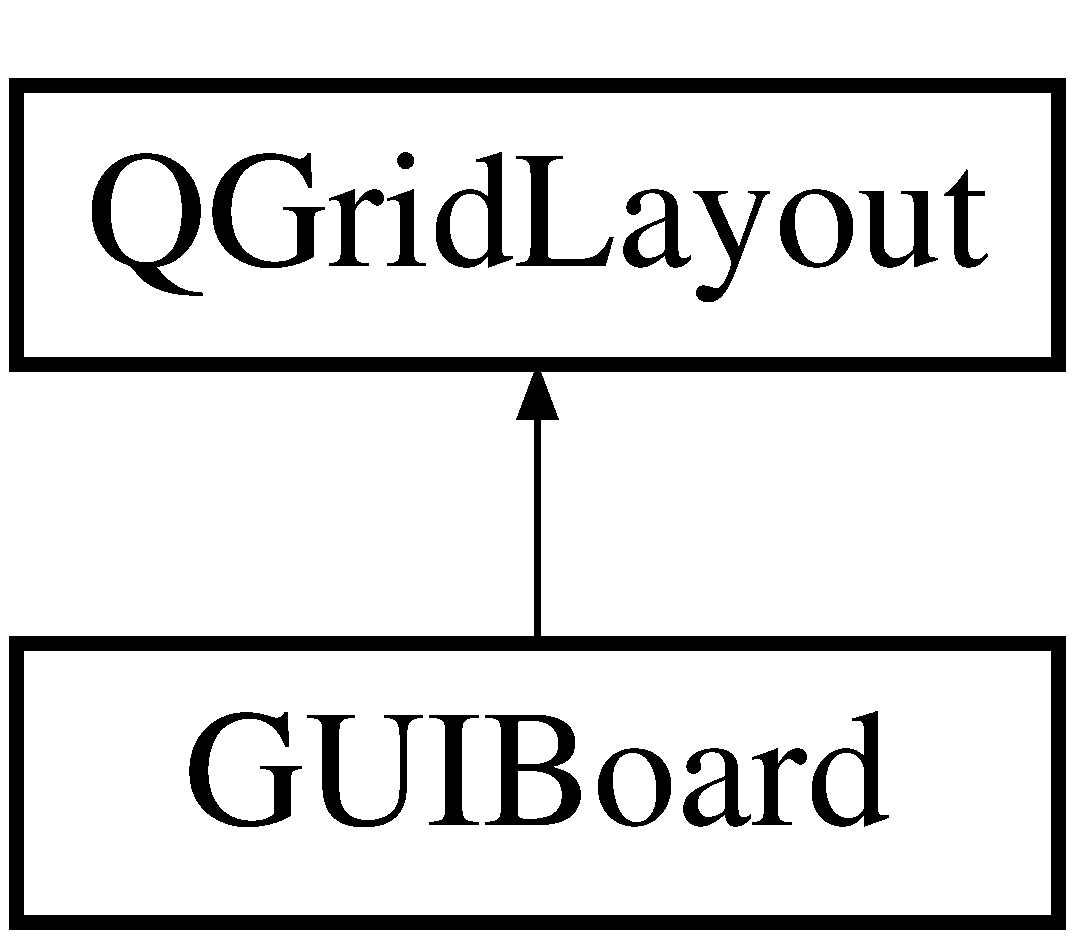
\includegraphics[height=2.000000cm]{class_g_u_i_board}
\end{center}
\end{figure}
\subsection*{Public Member Functions}
\begin{DoxyCompactItemize}
\item 
\hyperlink{class_g_u_i_board_a55050277239ca0bd7bfedf36439701ee}{G\+U\+I\+Board} (int row, int col)
\begin{DoxyCompactList}\small\item\em \hyperlink{class_g_u_i_board}{G\+U\+I\+Board} Build a new G\+UI \hyperlink{class_board}{Board}. \end{DoxyCompactList}\item 
void \hyperlink{class_g_u_i_board_a3e2ddf4a20541fed420ad1527e33c68a}{refresh\+Board} (\hyperlink{class_game}{Game} $\ast$game)
\begin{DoxyCompactList}\small\item\em refresh\+Board Update the board with a given game. \end{DoxyCompactList}\item 
void \hyperlink{class_g_u_i_board_aa6fd17a421d1b896a357e30c0cfe349d}{refresh\+Board\+End\+Game} (\hyperlink{class_game}{Game} $\ast$game)
\begin{DoxyCompactList}\small\item\em refresh\+Board\+End\+Game Updates the board by checking if the player had put a flag on a bomb. If so, a special image of a crossed bomb is put in the case. \end{DoxyCompactList}\end{DoxyCompactItemize}


\subsection{Detailed Description}
The \hyperlink{class_g_u_i_board}{G\+U\+I\+Board} class Represents a board graphically. 

Definition at line 12 of file guiboard.\+h.



\subsection{Constructor \& Destructor Documentation}
\mbox{\Hypertarget{class_g_u_i_board_a55050277239ca0bd7bfedf36439701ee}\label{class_g_u_i_board_a55050277239ca0bd7bfedf36439701ee}} 
\index{G\+U\+I\+Board@{G\+U\+I\+Board}!G\+U\+I\+Board@{G\+U\+I\+Board}}
\index{G\+U\+I\+Board@{G\+U\+I\+Board}!G\+U\+I\+Board@{G\+U\+I\+Board}}
\subsubsection{\texorpdfstring{G\+U\+I\+Board()}{GUIBoard()}}
{\footnotesize\ttfamily G\+U\+I\+Board\+::\+G\+U\+I\+Board (\begin{DoxyParamCaption}\item[{int}]{row,  }\item[{int}]{col }\end{DoxyParamCaption})}



\hyperlink{class_g_u_i_board}{G\+U\+I\+Board} Build a new G\+UI \hyperlink{class_board}{Board}. 


\begin{DoxyParams}{Parameters}
{\em row} & The number of row. \\
\hline
{\em col} & The number of column. \\
\hline
\end{DoxyParams}


Definition at line 4 of file guiboard.\+cpp.



\subsection{Member Function Documentation}
\mbox{\Hypertarget{class_g_u_i_board_a3e2ddf4a20541fed420ad1527e33c68a}\label{class_g_u_i_board_a3e2ddf4a20541fed420ad1527e33c68a}} 
\index{G\+U\+I\+Board@{G\+U\+I\+Board}!refresh\+Board@{refresh\+Board}}
\index{refresh\+Board@{refresh\+Board}!G\+U\+I\+Board@{G\+U\+I\+Board}}
\subsubsection{\texorpdfstring{refresh\+Board()}{refreshBoard()}}
{\footnotesize\ttfamily void G\+U\+I\+Board\+::refresh\+Board (\begin{DoxyParamCaption}\item[{\hyperlink{class_game}{Game} $\ast$}]{game }\end{DoxyParamCaption})}



refresh\+Board Update the board with a given game. 


\begin{DoxyParams}{Parameters}
{\em game} & The game the board has to print. \\
\hline
\end{DoxyParams}


Definition at line 23 of file guiboard.\+cpp.

\mbox{\Hypertarget{class_g_u_i_board_aa6fd17a421d1b896a357e30c0cfe349d}\label{class_g_u_i_board_aa6fd17a421d1b896a357e30c0cfe349d}} 
\index{G\+U\+I\+Board@{G\+U\+I\+Board}!refresh\+Board\+End\+Game@{refresh\+Board\+End\+Game}}
\index{refresh\+Board\+End\+Game@{refresh\+Board\+End\+Game}!G\+U\+I\+Board@{G\+U\+I\+Board}}
\subsubsection{\texorpdfstring{refresh\+Board\+End\+Game()}{refreshBoardEndGame()}}
{\footnotesize\ttfamily void G\+U\+I\+Board\+::refresh\+Board\+End\+Game (\begin{DoxyParamCaption}\item[{\hyperlink{class_game}{Game} $\ast$}]{game }\end{DoxyParamCaption})}



refresh\+Board\+End\+Game Updates the board by checking if the player had put a flag on a bomb. If so, a special image of a crossed bomb is put in the case. 


\begin{DoxyParams}{Parameters}
{\em game} & The game the board has to print. \\
\hline
\end{DoxyParams}


Definition at line 30 of file guiboard.\+cpp.



The documentation for this class was generated from the following files\+:\begin{DoxyCompactItemize}
\item 
Application/guiboard.\+h\item 
Application/guiboard.\+cpp\end{DoxyCompactItemize}

\hypertarget{class_g_u_i_screen}{}\section{G\+U\+I\+Screen Class Reference}
\label{class_g_u_i_screen}\index{G\+U\+I\+Screen@{G\+U\+I\+Screen}}


The \hyperlink{class_g_u_i_screen}{G\+U\+I\+Screen} class Represents a Mine\+Sweeper application.  




{\ttfamily \#include $<$guiscreen.\+h$>$}

Inheritance diagram for G\+U\+I\+Screen\+:\begin{figure}[H]
\begin{center}
\leavevmode
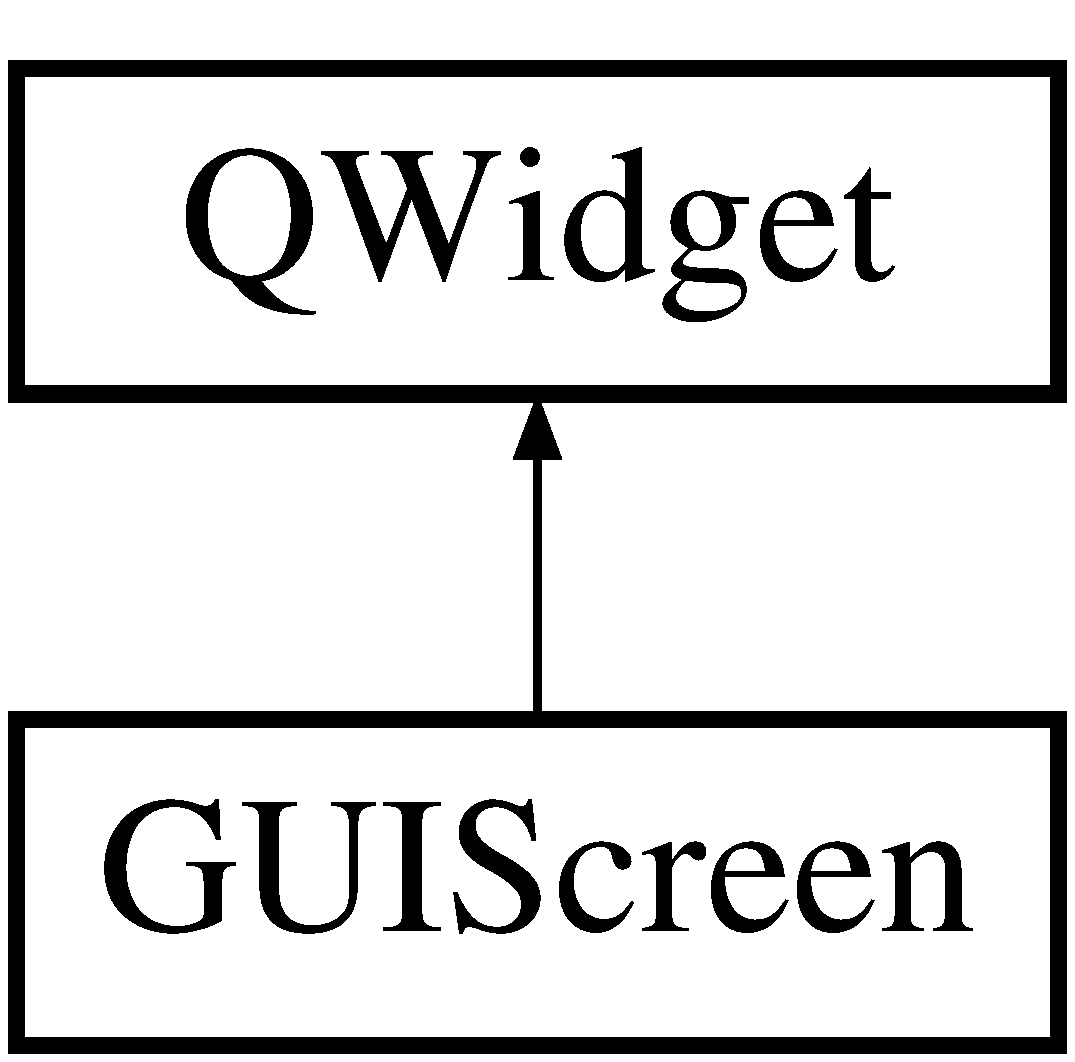
\includegraphics[height=2.000000cm]{class_g_u_i_screen}
\end{center}
\end{figure}
\subsection*{Public Member Functions}
\begin{DoxyCompactItemize}
\item 
\hyperlink{class_g_u_i_screen_aade2245bd739d9cd5cb667751c20dc05}{G\+U\+I\+Screen} (Q\+Widget $\ast$parent=0)
\begin{DoxyCompactList}\small\item\em \hyperlink{class_g_u_i_screen}{G\+U\+I\+Screen} Build a new Mine\+Sweeper application. \end{DoxyCompactList}\item 
void \hyperlink{class_g_u_i_screen_a02f2d6be64e2734c5a2cad7dc30689c1}{set\+Controller} (\hyperlink{class_controller}{Controller} $\ast$controller)
\begin{DoxyCompactList}\small\item\em set\+Controller Set the controller for the application. \end{DoxyCompactList}\end{DoxyCompactItemize}


\subsection{Detailed Description}
The \hyperlink{class_g_u_i_screen}{G\+U\+I\+Screen} class Represents a Mine\+Sweeper application. 

Definition at line 15 of file guiscreen.\+h.



\subsection{Constructor \& Destructor Documentation}
\mbox{\Hypertarget{class_g_u_i_screen_aade2245bd739d9cd5cb667751c20dc05}\label{class_g_u_i_screen_aade2245bd739d9cd5cb667751c20dc05}} 
\index{G\+U\+I\+Screen@{G\+U\+I\+Screen}!G\+U\+I\+Screen@{G\+U\+I\+Screen}}
\index{G\+U\+I\+Screen@{G\+U\+I\+Screen}!G\+U\+I\+Screen@{G\+U\+I\+Screen}}
\subsubsection{\texorpdfstring{G\+U\+I\+Screen()}{GUIScreen()}}
{\footnotesize\ttfamily G\+U\+I\+Screen\+::\+G\+U\+I\+Screen (\begin{DoxyParamCaption}\item[{Q\+Widget $\ast$}]{parent = {\ttfamily 0} }\end{DoxyParamCaption})\hspace{0.3cm}{\ttfamily [explicit]}}



\hyperlink{class_g_u_i_screen}{G\+U\+I\+Screen} Build a new Mine\+Sweeper application. 


\begin{DoxyParams}{Parameters}
{\em parent} & \\
\hline
\end{DoxyParams}


Definition at line 15 of file guiscreen.\+cpp.



\subsection{Member Function Documentation}
\mbox{\Hypertarget{class_g_u_i_screen_a02f2d6be64e2734c5a2cad7dc30689c1}\label{class_g_u_i_screen_a02f2d6be64e2734c5a2cad7dc30689c1}} 
\index{G\+U\+I\+Screen@{G\+U\+I\+Screen}!set\+Controller@{set\+Controller}}
\index{set\+Controller@{set\+Controller}!G\+U\+I\+Screen@{G\+U\+I\+Screen}}
\subsubsection{\texorpdfstring{set\+Controller()}{setController()}}
{\footnotesize\ttfamily void G\+U\+I\+Screen\+::set\+Controller (\begin{DoxyParamCaption}\item[{\hyperlink{class_controller}{Controller} $\ast$}]{controller }\end{DoxyParamCaption})}



set\+Controller Set the controller for the application. 


\begin{DoxyParams}{Parameters}
{\em controller} & The new controller. \\
\hline
\end{DoxyParams}


Definition at line 49 of file guiscreen.\+cpp.



The documentation for this class was generated from the following files\+:\begin{DoxyCompactItemize}
\item 
Application/guiscreen.\+h\item 
Application/guiscreen.\+cpp\end{DoxyCompactItemize}

\hypertarget{class_ui_1_1_g_u_i_screen}{}\section{Ui\+:\+:G\+U\+I\+Screen Class Reference}
\label{class_ui_1_1_g_u_i_screen}\index{Ui\+::\+G\+U\+I\+Screen@{Ui\+::\+G\+U\+I\+Screen}}
Inheritance diagram for Ui\+:\+:G\+U\+I\+Screen\+:\begin{figure}[H]
\begin{center}
\leavevmode
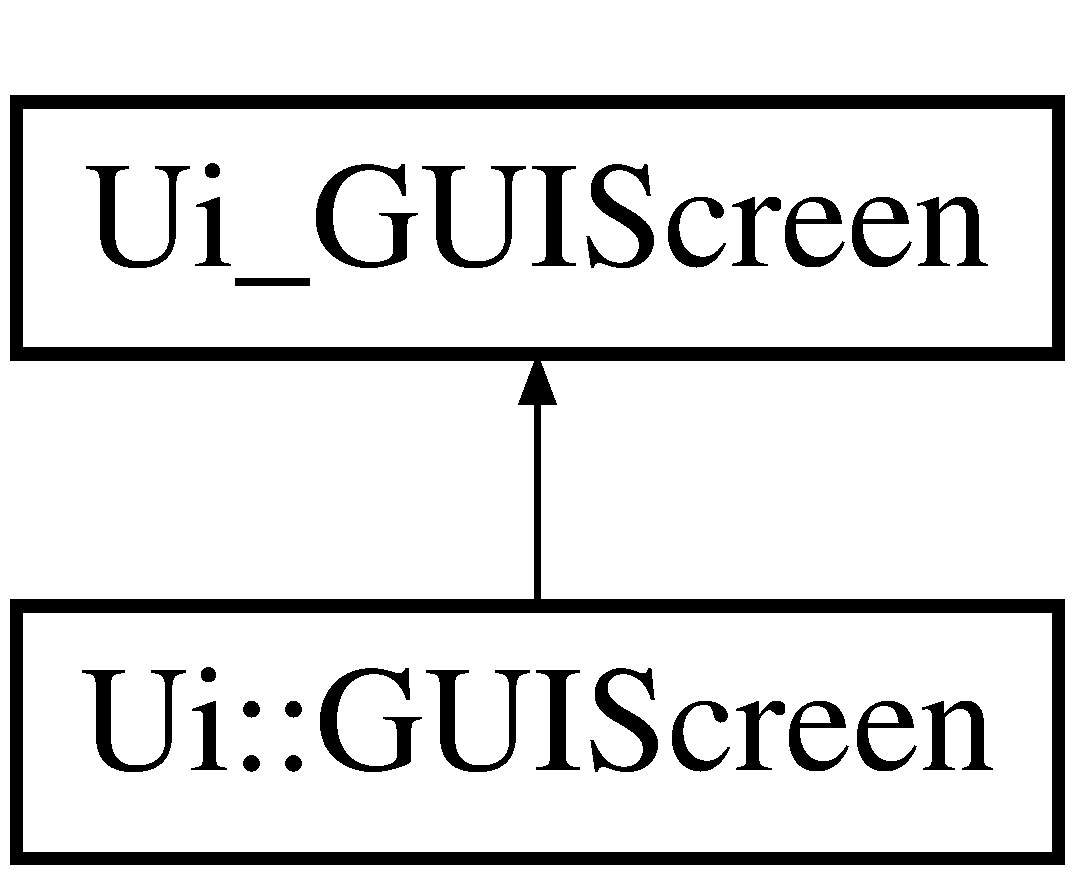
\includegraphics[height=2.000000cm]{class_ui_1_1_g_u_i_screen}
\end{center}
\end{figure}
\subsection*{Additional Inherited Members}


\subsection{Detailed Description}


Definition at line 417 of file ui\+\_\+guiscreen.\+h.



The documentation for this class was generated from the following file\+:\begin{DoxyCompactItemize}
\item 
Application/ui\+\_\+guiscreen.\+h\end{DoxyCompactItemize}

\hypertarget{class_hall_of_fame}{}\section{Hall\+Of\+Fame Class Reference}
\label{class_hall_of_fame}\index{Hall\+Of\+Fame@{Hall\+Of\+Fame}}


The \hyperlink{class_hall_of_fame}{Hall\+Of\+Fame} class Represents all the top 5 for all the different type of board. For each triplet (height, width, nb\+Bombs), there is a top5.  




{\ttfamily \#include $<$halloffame.\+h$>$}

\subsection*{Public Member Functions}
\begin{DoxyCompactItemize}
\item 
\mbox{\Hypertarget{class_hall_of_fame_a158b9ebd9094021024497bd5f3e04199}\label{class_hall_of_fame_a158b9ebd9094021024497bd5f3e04199}} 
\hyperlink{class_hall_of_fame_a158b9ebd9094021024497bd5f3e04199}{Hall\+Of\+Fame} ()
\begin{DoxyCompactList}\small\item\em \hyperlink{class_hall_of_fame}{Hall\+Of\+Fame} It creates an instance of the class from nothing. \end{DoxyCompactList}\item 
\mbox{\Hypertarget{class_hall_of_fame_a5960b73dc9e85927117541675c855ca7}\label{class_hall_of_fame_a5960b73dc9e85927117541675c855ca7}} 
\hyperlink{class_hall_of_fame_a5960b73dc9e85927117541675c855ca7}{$\sim$\+Hall\+Of\+Fame} ()
\begin{DoxyCompactList}\small\item\em The destructor Deletes all the elements from the class that need to be deleted. \end{DoxyCompactList}\item 
\mbox{\Hypertarget{class_hall_of_fame_a9ce6a64635d9087f0bce2f6b911918ab}\label{class_hall_of_fame_a9ce6a64635d9087f0bce2f6b911918ab}} 
void \hyperlink{class_hall_of_fame_a9ce6a64635d9087f0bce2f6b911918ab}{init\+Map\+Score} ()
\begin{DoxyCompactList}\small\item\em init\+Map\+Score Read all the data (height, width, nb\+Bombs, name of player, time (for 1 game)) in a file (.txt) Copy them all into scores, a map, the attribute of the class. \end{DoxyCompactList}\item 
void \hyperlink{class_hall_of_fame_af27ed4518905f0a948112a05268ffd73}{add\+Score} (const \hyperlink{struct_board_type}{Board\+Type} \&board\+Type, const \hyperlink{class_score}{Score} \&score)
\begin{DoxyCompactList}\small\item\em add\+Score Adds a \hyperlink{class_score}{Score} (structure composed of the name of the player and its time) into the map. \end{DoxyCompactList}\item 
\textbf{ std\+::vector}$<$ \hyperlink{class_score}{Score} $>$ \hyperlink{class_hall_of_fame_aa5df9550ea310ad6d72c55c0656213a0}{get\+Top} (const \hyperlink{struct_board_type}{Board\+Type} \&board\+Type)
\begin{DoxyCompactList}\small\item\em get\+Top Returns the top (list of 5 bests times) for a given \hyperlink{struct_board_type}{Board\+Type}. \end{DoxyCompactList}\item 
\textbf{ std\+::vector}$<$ \hyperlink{class_score}{Score} $>$ \hyperlink{class_hall_of_fame_ade9732fe195179e6ff7a7adecf2f4528}{get\+Top} (int index)
\begin{DoxyCompactList}\small\item\em get\+Top Returns the top (list of 5 bests times) for a given index. \end{DoxyCompactList}\item 
\mbox{\Hypertarget{class_hall_of_fame_a84804f031deb3f4ef290bce0c6f84db9}\label{class_hall_of_fame_a84804f031deb3f4ef290bce0c6f84db9}} 
void \hyperlink{class_hall_of_fame_a84804f031deb3f4ef290bce0c6f84db9}{write\+File} ()
\begin{DoxyCompactList}\small\item\em write\+File Writes into a file the content of the map. We do that in order to save the scores and then keep an history of the best scores. \end{DoxyCompactList}\item 
\textbf{ std\+::vector}$<$ \textbf{ std\+::string} $>$ \hyperlink{class_hall_of_fame_aa784fe5d8ace8fb5b2344a06bfb5fb84}{get\+Keys} ()
\begin{DoxyCompactList}\small\item\em get\+Keys Get all the boardtype on which it exists a top. \end{DoxyCompactList}\end{DoxyCompactItemize}


\subsection{Detailed Description}
The \hyperlink{class_hall_of_fame}{Hall\+Of\+Fame} class Represents all the top 5 for all the different type of board. For each triplet (height, width, nb\+Bombs), there is a top5. 

Definition at line 13 of file halloffame.\+h.



\subsection{Member Function Documentation}
\mbox{\Hypertarget{class_hall_of_fame_af27ed4518905f0a948112a05268ffd73}\label{class_hall_of_fame_af27ed4518905f0a948112a05268ffd73}} 
\index{Hall\+Of\+Fame@{Hall\+Of\+Fame}!add\+Score@{add\+Score}}
\index{add\+Score@{add\+Score}!Hall\+Of\+Fame@{Hall\+Of\+Fame}}
\subsubsection{\texorpdfstring{add\+Score()}{addScore()}}
{\footnotesize\ttfamily void Hall\+Of\+Fame\+::add\+Score (\begin{DoxyParamCaption}\item[{const \hyperlink{struct_board_type}{Board\+Type} \&}]{board\+Type,  }\item[{const \hyperlink{class_score}{Score} \&}]{score }\end{DoxyParamCaption})}



add\+Score Adds a \hyperlink{class_score}{Score} (structure composed of the name of the player and its time) into the map. 


\begin{DoxyParams}{Parameters}
{\em board\+Type} & The \hyperlink{struct_board_type}{Board\+Type} (height, width and nb\+Bombs of the board) \\
\hline
{\em score} & the \hyperlink{class_score}{Score} (name and time). \\
\hline
\end{DoxyParams}


Definition at line 15 of file halloffame.\+cpp.

\mbox{\Hypertarget{class_hall_of_fame_aa784fe5d8ace8fb5b2344a06bfb5fb84}\label{class_hall_of_fame_aa784fe5d8ace8fb5b2344a06bfb5fb84}} 
\index{Hall\+Of\+Fame@{Hall\+Of\+Fame}!get\+Keys@{get\+Keys}}
\index{get\+Keys@{get\+Keys}!Hall\+Of\+Fame@{Hall\+Of\+Fame}}
\subsubsection{\texorpdfstring{get\+Keys()}{getKeys()}}
{\footnotesize\ttfamily \textbf{ vector}$<$ \textbf{ string} $>$ Hall\+Of\+Fame\+::get\+Keys (\begin{DoxyParamCaption}{ }\end{DoxyParamCaption})}



get\+Keys Get all the boardtype on which it exists a top. 

\begin{DoxyReturn}{Returns}
All the board\+Type on which it exists a top. 
\end{DoxyReturn}


Definition at line 182 of file halloffame.\+cpp.

\mbox{\Hypertarget{class_hall_of_fame_aa5df9550ea310ad6d72c55c0656213a0}\label{class_hall_of_fame_aa5df9550ea310ad6d72c55c0656213a0}} 
\index{Hall\+Of\+Fame@{Hall\+Of\+Fame}!get\+Top@{get\+Top}}
\index{get\+Top@{get\+Top}!Hall\+Of\+Fame@{Hall\+Of\+Fame}}
\subsubsection{\texorpdfstring{get\+Top()}{getTop()}\hspace{0.1cm}{\footnotesize\ttfamily [1/2]}}
{\footnotesize\ttfamily \textbf{ std\+::vector}$<$ \hyperlink{class_score}{Score} $>$ Hall\+Of\+Fame\+::get\+Top (\begin{DoxyParamCaption}\item[{const \hyperlink{struct_board_type}{Board\+Type} \&}]{board\+Type }\end{DoxyParamCaption})}



get\+Top Returns the top (list of 5 bests times) for a given \hyperlink{struct_board_type}{Board\+Type}. 


\begin{DoxyParams}{Parameters}
{\em board\+Type} & the \hyperlink{struct_board_type}{Board\+Type}. \\
\hline
\end{DoxyParams}
\begin{DoxyReturn}{Returns}
a vector of \hyperlink{class_score}{Score}, the top 5 linked to the given \hyperlink{struct_board_type}{Board\+Type}. 
\end{DoxyReturn}


Definition at line 54 of file halloffame.\+cpp.

\mbox{\Hypertarget{class_hall_of_fame_ade9732fe195179e6ff7a7adecf2f4528}\label{class_hall_of_fame_ade9732fe195179e6ff7a7adecf2f4528}} 
\index{Hall\+Of\+Fame@{Hall\+Of\+Fame}!get\+Top@{get\+Top}}
\index{get\+Top@{get\+Top}!Hall\+Of\+Fame@{Hall\+Of\+Fame}}
\subsubsection{\texorpdfstring{get\+Top()}{getTop()}\hspace{0.1cm}{\footnotesize\ttfamily [2/2]}}
{\footnotesize\ttfamily \textbf{ std\+::vector}$<$ \hyperlink{class_score}{Score} $>$ Hall\+Of\+Fame\+::get\+Top (\begin{DoxyParamCaption}\item[{int}]{index }\end{DoxyParamCaption})}



get\+Top Returns the top (list of 5 bests times) for a given index. 


\begin{DoxyParams}{Parameters}
{\em index} & The index of the top in the map. \\
\hline
\end{DoxyParams}
\begin{DoxyReturn}{Returns}
a vector of \hyperlink{class_score}{Score}, the top 5 linked to the given index. 
\end{DoxyReturn}


Definition at line 63 of file halloffame.\+cpp.



The documentation for this class was generated from the following files\+:\begin{DoxyCompactItemize}
\item 
Application/halloffame.\+h\item 
Application/halloffame.\+cpp\end{DoxyCompactItemize}

\hypertarget{struct_catch_1_1_i_context}{}\section{Catch\+:\+:I\+Context Struct Reference}
\label{struct_catch_1_1_i_context}\index{Catch\+::\+I\+Context@{Catch\+::\+I\+Context}}
Inheritance diagram for Catch\+:\+:I\+Context\+:\begin{figure}[H]
\begin{center}
\leavevmode
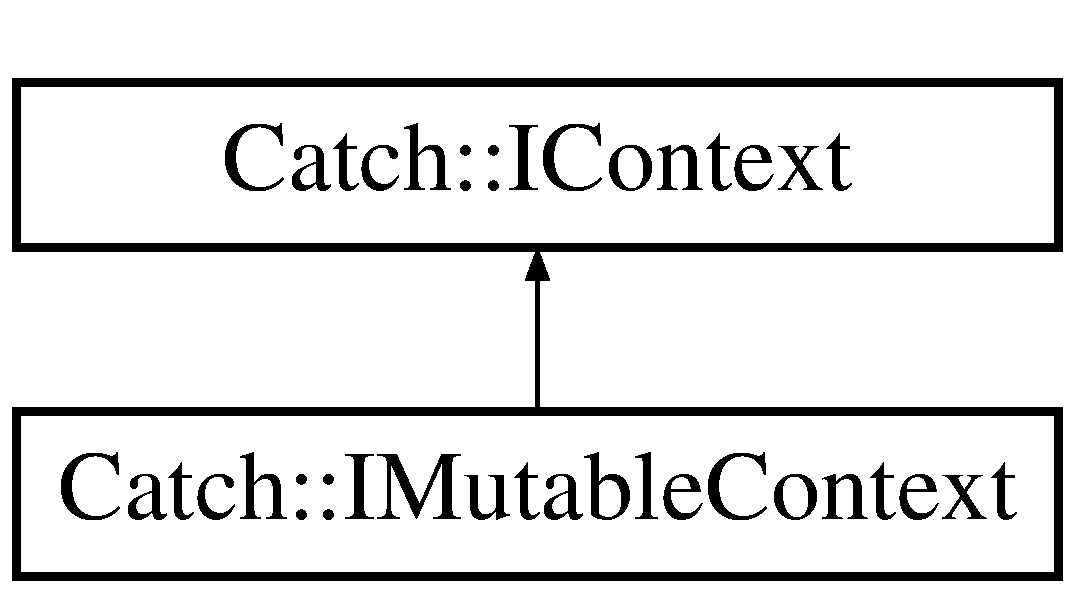
\includegraphics[height=2.000000cm]{struct_catch_1_1_i_context}
\end{center}
\end{figure}
\subsection*{Public Member Functions}
\begin{DoxyCompactItemize}
\item 
\mbox{\Hypertarget{struct_catch_1_1_i_context_a684e4ae71d1fdf3060c352ecde1d122f}\label{struct_catch_1_1_i_context_a684e4ae71d1fdf3060c352ecde1d122f}} 
virtual \hyperlink{struct_catch_1_1_i_result_capture}{I\+Result\+Capture} $\ast$ {\bfseries get\+Result\+Capture} ()=0
\item 
\mbox{\Hypertarget{struct_catch_1_1_i_context_af088415dde18d039ed5a2f95b02767c6}\label{struct_catch_1_1_i_context_af088415dde18d039ed5a2f95b02767c6}} 
virtual \hyperlink{struct_catch_1_1_i_runner}{I\+Runner} $\ast$ {\bfseries get\+Runner} ()=0
\item 
\mbox{\Hypertarget{struct_catch_1_1_i_context_a43e07088db43299ba129fbe6d3106e95}\label{struct_catch_1_1_i_context_a43e07088db43299ba129fbe6d3106e95}} 
virtual size\+\_\+t {\bfseries get\+Generator\+Index} (\textbf{ std\+::string} const \&file\+Info, size\+\_\+t total\+Size)=0
\item 
\mbox{\Hypertarget{struct_catch_1_1_i_context_a806f7c4ed24d51adae90418e661b24b7}\label{struct_catch_1_1_i_context_a806f7c4ed24d51adae90418e661b24b7}} 
virtual bool {\bfseries advance\+Generators\+For\+Current\+Test} ()=0
\item 
\mbox{\Hypertarget{struct_catch_1_1_i_context_aee81c415899262e096ad8d6f686fa365}\label{struct_catch_1_1_i_context_aee81c415899262e096ad8d6f686fa365}} 
virtual \hyperlink{class_catch_1_1_ptr}{Ptr}$<$ I\+Config const  $>$ {\bfseries get\+Config} () const =0
\end{DoxyCompactItemize}


\subsection{Detailed Description}


Definition at line 543 of file catch.\+hpp.



The documentation for this struct was generated from the following file\+:\begin{DoxyCompactItemize}
\item 
Tests/catch.\+hpp\end{DoxyCompactItemize}

\hypertarget{struct_catch_1_1_i_exception_translator}{}\section{Catch\+:\+:I\+Exception\+Translator Struct Reference}
\label{struct_catch_1_1_i_exception_translator}\index{Catch\+::\+I\+Exception\+Translator@{Catch\+::\+I\+Exception\+Translator}}
\subsection*{Public Member Functions}
\begin{DoxyCompactItemize}
\item 
\mbox{\Hypertarget{struct_catch_1_1_i_exception_translator_a2a554b96ed5ed411e7c796b6b42837a5}\label{struct_catch_1_1_i_exception_translator_a2a554b96ed5ed411e7c796b6b42837a5}} 
virtual \textbf{ std\+::string} {\bfseries translate} (Exception\+Translators\+::const\+\_\+iterator it, Exception\+Translators\+::const\+\_\+iterator it\+End) const =0
\end{DoxyCompactItemize}


\subsection{Detailed Description}


Definition at line 2520 of file catch.\+hpp.



The documentation for this struct was generated from the following file\+:\begin{DoxyCompactItemize}
\item 
Tests/catch.\+hpp\end{DoxyCompactItemize}

\hypertarget{struct_catch_1_1_i_exception_translator_registry}{}\section{Catch\+:\+:I\+Exception\+Translator\+Registry Struct Reference}
\label{struct_catch_1_1_i_exception_translator_registry}\index{Catch\+::\+I\+Exception\+Translator\+Registry@{Catch\+::\+I\+Exception\+Translator\+Registry}}
\subsection*{Public Member Functions}
\begin{DoxyCompactItemize}
\item 
\mbox{\Hypertarget{struct_catch_1_1_i_exception_translator_registry_af76ae8c331a17f2a94c9720bc0d686bb}\label{struct_catch_1_1_i_exception_translator_registry_af76ae8c331a17f2a94c9720bc0d686bb}} 
virtual \textbf{ std\+::string} {\bfseries translate\+Active\+Exception} () const =0
\end{DoxyCompactItemize}


\subsection{Detailed Description}


Definition at line 2525 of file catch.\+hpp.



The documentation for this struct was generated from the following file\+:\begin{DoxyCompactItemize}
\item 
Tests/catch.\+hpp\end{DoxyCompactItemize}

\hypertarget{struct_catch_1_1_i_generator}{}\section{Catch\+:\+:I\+Generator$<$ T $>$ Struct Template Reference}
\label{struct_catch_1_1_i_generator}\index{Catch\+::\+I\+Generator$<$ T $>$@{Catch\+::\+I\+Generator$<$ T $>$}}
Inheritance diagram for Catch\+:\+:I\+Generator$<$ T $>$\+:\begin{figure}[H]
\begin{center}
\leavevmode
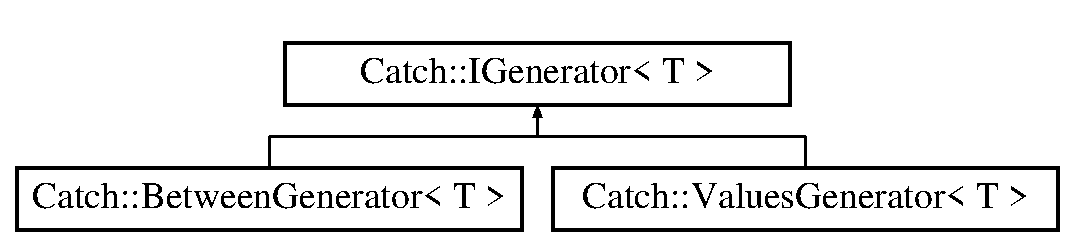
\includegraphics[height=2.000000cm]{struct_catch_1_1_i_generator}
\end{center}
\end{figure}
\subsection*{Public Member Functions}
\begin{DoxyCompactItemize}
\item 
\mbox{\Hypertarget{struct_catch_1_1_i_generator_ad69e937cb66dba3ed9429c42abf4fce3}\label{struct_catch_1_1_i_generator_ad69e937cb66dba3ed9429c42abf4fce3}} 
virtual T {\bfseries get\+Value} (\textbf{ std\+::size\+\_\+t} index) const =0
\item 
\mbox{\Hypertarget{struct_catch_1_1_i_generator_a2e317253b03e838b6065ce69719a198e}\label{struct_catch_1_1_i_generator_a2e317253b03e838b6065ce69719a198e}} 
virtual \textbf{ std\+::size\+\_\+t} {\bfseries size} () const =0
\end{DoxyCompactItemize}


\subsection{Detailed Description}
\subsubsection*{template$<$typename T$>$\newline
struct Catch\+::\+I\+Generator$<$ T $>$}



Definition at line 2301 of file catch.\+hpp.



The documentation for this struct was generated from the following file\+:\begin{DoxyCompactItemize}
\item 
Tests/catch.\+hpp\end{DoxyCompactItemize}

\hypertarget{struct_catch_1_1_i_generator_info}{}\section{Catch\+:\+:I\+Generator\+Info Struct Reference}
\label{struct_catch_1_1_i_generator_info}\index{Catch\+::\+I\+Generator\+Info@{Catch\+::\+I\+Generator\+Info}}
\subsection*{Public Member Functions}
\begin{DoxyCompactItemize}
\item 
\mbox{\Hypertarget{struct_catch_1_1_i_generator_info_a2b86711ca7009903edfe27ed62b515ef}\label{struct_catch_1_1_i_generator_info_a2b86711ca7009903edfe27ed62b515ef}} 
virtual bool {\bfseries move\+Next} ()=0
\item 
\mbox{\Hypertarget{struct_catch_1_1_i_generator_info_a6a0dca712d31f6849fd9447b1344673a}\label{struct_catch_1_1_i_generator_info_a6a0dca712d31f6849fd9447b1344673a}} 
virtual \textbf{ std\+::size\+\_\+t} {\bfseries get\+Current\+Index} () const =0
\end{DoxyCompactItemize}


\subsection{Detailed Description}


Definition at line 430 of file catch.\+hpp.



The documentation for this struct was generated from the following file\+:\begin{DoxyCompactItemize}
\item 
Tests/catch.\+hpp\end{DoxyCompactItemize}

\hypertarget{struct_catch_1_1_i_generators_for_test}{}\section{Catch\+:\+:I\+Generators\+For\+Test Struct Reference}
\label{struct_catch_1_1_i_generators_for_test}\index{Catch\+::\+I\+Generators\+For\+Test@{Catch\+::\+I\+Generators\+For\+Test}}
\subsection*{Public Member Functions}
\begin{DoxyCompactItemize}
\item 
\mbox{\Hypertarget{struct_catch_1_1_i_generators_for_test_a180d84e858840188e4c3788e47eefdb0}\label{struct_catch_1_1_i_generators_for_test_a180d84e858840188e4c3788e47eefdb0}} 
virtual \hyperlink{struct_catch_1_1_i_generator_info}{I\+Generator\+Info} \& {\bfseries get\+Generator\+Info} (\textbf{ std\+::string} const \&file\+Info, \textbf{ std\+::size\+\_\+t} size)=0
\item 
\mbox{\Hypertarget{struct_catch_1_1_i_generators_for_test_adab31832d529fc584fd63164e0a1c8ad}\label{struct_catch_1_1_i_generators_for_test_adab31832d529fc584fd63164e0a1c8ad}} 
virtual bool {\bfseries move\+Next} ()=0
\end{DoxyCompactItemize}


\subsection{Detailed Description}


Definition at line 436 of file catch.\+hpp.



The documentation for this struct was generated from the following file\+:\begin{DoxyCompactItemize}
\item 
Tests/catch.\+hpp\end{DoxyCompactItemize}

\hypertarget{struct_catch_1_1_i_mutable_context}{}\section{Catch\+:\+:I\+Mutable\+Context Struct Reference}
\label{struct_catch_1_1_i_mutable_context}\index{Catch\+::\+I\+Mutable\+Context@{Catch\+::\+I\+Mutable\+Context}}
Inheritance diagram for Catch\+:\+:I\+Mutable\+Context\+:\begin{figure}[H]
\begin{center}
\leavevmode
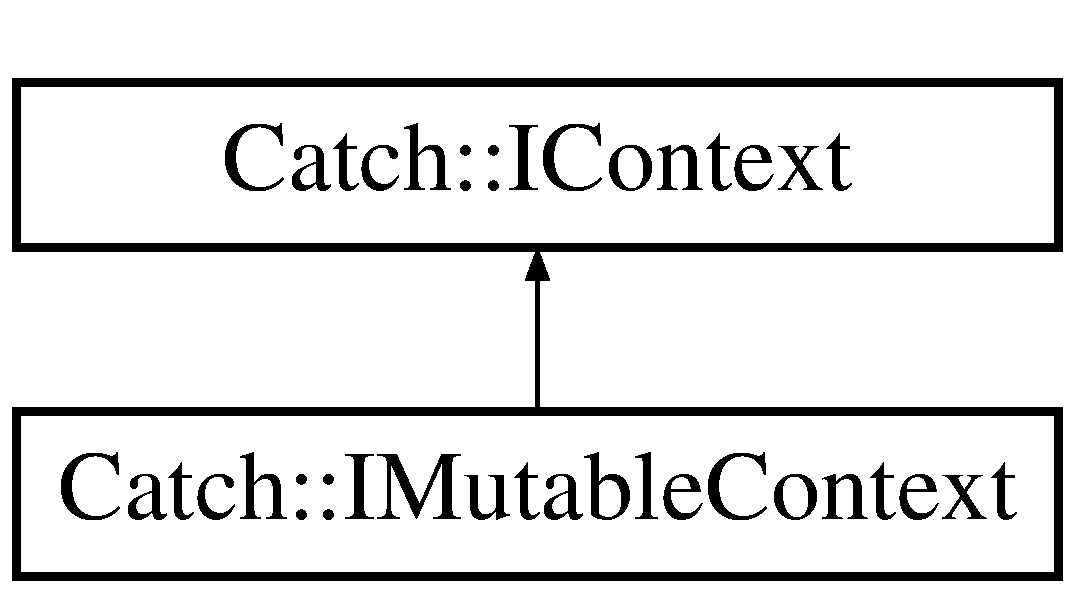
\includegraphics[height=2.000000cm]{struct_catch_1_1_i_mutable_context}
\end{center}
\end{figure}
\subsection*{Public Member Functions}
\begin{DoxyCompactItemize}
\item 
\mbox{\Hypertarget{struct_catch_1_1_i_mutable_context_a4a80afd0525b7def21bee8d9b48f2d39}\label{struct_catch_1_1_i_mutable_context_a4a80afd0525b7def21bee8d9b48f2d39}} 
virtual void {\bfseries set\+Result\+Capture} (\hyperlink{struct_catch_1_1_i_result_capture}{I\+Result\+Capture} $\ast$result\+Capture)=0
\item 
\mbox{\Hypertarget{struct_catch_1_1_i_mutable_context_af2e53b1dea4527a2587cff266a730f6e}\label{struct_catch_1_1_i_mutable_context_af2e53b1dea4527a2587cff266a730f6e}} 
virtual void {\bfseries set\+Runner} (\hyperlink{struct_catch_1_1_i_runner}{I\+Runner} $\ast$runner)=0
\item 
\mbox{\Hypertarget{struct_catch_1_1_i_mutable_context_a013e8f688a8ea7970262d07ead542a63}\label{struct_catch_1_1_i_mutable_context_a013e8f688a8ea7970262d07ead542a63}} 
virtual void {\bfseries set\+Config} (\hyperlink{class_catch_1_1_ptr}{Ptr}$<$ I\+Config const $>$ const \&config)=0
\end{DoxyCompactItemize}


\subsection{Detailed Description}


Definition at line 554 of file catch.\+hpp.



The documentation for this struct was generated from the following file\+:\begin{DoxyCompactItemize}
\item 
Tests/catch.\+hpp\end{DoxyCompactItemize}

\hypertarget{struct_catch_1_1_i_mutable_registry_hub}{}\section{Catch\+:\+:I\+Mutable\+Registry\+Hub Struct Reference}
\label{struct_catch_1_1_i_mutable_registry_hub}\index{Catch\+::\+I\+Mutable\+Registry\+Hub@{Catch\+::\+I\+Mutable\+Registry\+Hub}}
\subsection*{Public Member Functions}
\begin{DoxyCompactItemize}
\item 
\mbox{\Hypertarget{struct_catch_1_1_i_mutable_registry_hub_aab72d0aa1fa14627f1a6a4c893ae0a12}\label{struct_catch_1_1_i_mutable_registry_hub_aab72d0aa1fa14627f1a6a4c893ae0a12}} 
virtual void {\bfseries register\+Reporter} (\textbf{ std\+::string} const \&name, \hyperlink{class_catch_1_1_ptr}{Ptr}$<$ I\+Reporter\+Factory $>$ const \&factory)=0
\item 
\mbox{\Hypertarget{struct_catch_1_1_i_mutable_registry_hub_ae06fcb90ba3f2b389d450cd81e229276}\label{struct_catch_1_1_i_mutable_registry_hub_ae06fcb90ba3f2b389d450cd81e229276}} 
virtual void {\bfseries register\+Listener} (\hyperlink{class_catch_1_1_ptr}{Ptr}$<$ I\+Reporter\+Factory $>$ const \&factory)=0
\item 
\mbox{\Hypertarget{struct_catch_1_1_i_mutable_registry_hub_a11b85c6744d88c9f83fe16ad4a8dd451}\label{struct_catch_1_1_i_mutable_registry_hub_a11b85c6744d88c9f83fe16ad4a8dd451}} 
virtual void {\bfseries register\+Test} (\hyperlink{class_catch_1_1_test_case}{Test\+Case} const \&test\+Info)=0
\item 
\mbox{\Hypertarget{struct_catch_1_1_i_mutable_registry_hub_ae6825365102693cf7707db022a2c2b49}\label{struct_catch_1_1_i_mutable_registry_hub_ae6825365102693cf7707db022a2c2b49}} 
virtual void {\bfseries register\+Translator} (const \hyperlink{struct_catch_1_1_i_exception_translator}{I\+Exception\+Translator} $\ast$translator)=0
\end{DoxyCompactItemize}


\subsection{Detailed Description}


Definition at line 2498 of file catch.\+hpp.



The documentation for this struct was generated from the following file\+:\begin{DoxyCompactItemize}
\item 
Tests/catch.\+hpp\end{DoxyCompactItemize}

\hypertarget{struct_catch_1_1_i_registry_hub}{}\section{Catch\+:\+:I\+Registry\+Hub Struct Reference}
\label{struct_catch_1_1_i_registry_hub}\index{Catch\+::\+I\+Registry\+Hub@{Catch\+::\+I\+Registry\+Hub}}
\subsection*{Public Member Functions}
\begin{DoxyCompactItemize}
\item 
\mbox{\Hypertarget{struct_catch_1_1_i_registry_hub_a55534563f7ecf7e20ec1e37285ebe54d}\label{struct_catch_1_1_i_registry_hub_a55534563f7ecf7e20ec1e37285ebe54d}} 
virtual I\+Reporter\+Registry const  \& {\bfseries get\+Reporter\+Registry} () const =0
\item 
\mbox{\Hypertarget{struct_catch_1_1_i_registry_hub_af4f6255f0c0f8f1f179fa9d7d4843076}\label{struct_catch_1_1_i_registry_hub_af4f6255f0c0f8f1f179fa9d7d4843076}} 
virtual \hyperlink{struct_catch_1_1_i_test_case_registry}{I\+Test\+Case\+Registry} const  \& {\bfseries get\+Test\+Case\+Registry} () const =0
\item 
\mbox{\Hypertarget{struct_catch_1_1_i_registry_hub_a3606988da110c016c5af3ae63454eb78}\label{struct_catch_1_1_i_registry_hub_a3606988da110c016c5af3ae63454eb78}} 
virtual \hyperlink{struct_catch_1_1_i_exception_translator_registry}{I\+Exception\+Translator\+Registry} \& {\bfseries get\+Exception\+Translator\+Registry} ()=0
\end{DoxyCompactItemize}


\subsection{Detailed Description}


Definition at line 2490 of file catch.\+hpp.



The documentation for this struct was generated from the following file\+:\begin{DoxyCompactItemize}
\item 
Tests/catch.\+hpp\end{DoxyCompactItemize}

\hypertarget{struct_catch_1_1_i_result_capture}{}\section{Catch\+:\+:I\+Result\+Capture Struct Reference}
\label{struct_catch_1_1_i_result_capture}\index{Catch\+::\+I\+Result\+Capture@{Catch\+::\+I\+Result\+Capture}}
\subsection*{Public Member Functions}
\begin{DoxyCompactItemize}
\item 
\mbox{\Hypertarget{struct_catch_1_1_i_result_capture_ae45e08bccc5fb434656d4f2e44742223}\label{struct_catch_1_1_i_result_capture_ae45e08bccc5fb434656d4f2e44742223}} 
virtual void {\bfseries assertion\+Ended} (\hyperlink{class_catch_1_1_assertion_result}{Assertion\+Result} const \&result)=0
\item 
\mbox{\Hypertarget{struct_catch_1_1_i_result_capture_a5b76ed52badcb64cf374202e12b81a03}\label{struct_catch_1_1_i_result_capture_a5b76ed52badcb64cf374202e12b81a03}} 
virtual bool {\bfseries section\+Started} (\hyperlink{struct_catch_1_1_section_info}{Section\+Info} const \&section\+Info, \hyperlink{struct_catch_1_1_counts}{Counts} \&assertions)=0
\item 
\mbox{\Hypertarget{struct_catch_1_1_i_result_capture_a4e152bc43dc0933684e31fa67a58195d}\label{struct_catch_1_1_i_result_capture_a4e152bc43dc0933684e31fa67a58195d}} 
virtual void {\bfseries section\+Ended} (\hyperlink{struct_catch_1_1_section_end_info}{Section\+End\+Info} const \&end\+Info)=0
\item 
\mbox{\Hypertarget{struct_catch_1_1_i_result_capture_afcc71eef8ca821ae132cced4a2be6988}\label{struct_catch_1_1_i_result_capture_afcc71eef8ca821ae132cced4a2be6988}} 
virtual void {\bfseries section\+Ended\+Early} (\hyperlink{struct_catch_1_1_section_end_info}{Section\+End\+Info} const \&end\+Info)=0
\item 
\mbox{\Hypertarget{struct_catch_1_1_i_result_capture_a91d154c1e087e383dcde5aad95cb6a05}\label{struct_catch_1_1_i_result_capture_a91d154c1e087e383dcde5aad95cb6a05}} 
virtual void {\bfseries push\+Scoped\+Message} (\hyperlink{struct_catch_1_1_message_info}{Message\+Info} const \&message)=0
\item 
\mbox{\Hypertarget{struct_catch_1_1_i_result_capture_a42bcb13276706bf8c3ce081ce16d37fd}\label{struct_catch_1_1_i_result_capture_a42bcb13276706bf8c3ce081ce16d37fd}} 
virtual void {\bfseries pop\+Scoped\+Message} (\hyperlink{struct_catch_1_1_message_info}{Message\+Info} const \&message)=0
\item 
\mbox{\Hypertarget{struct_catch_1_1_i_result_capture_aea1617f4a84cc648246aa3ed6918b5bf}\label{struct_catch_1_1_i_result_capture_aea1617f4a84cc648246aa3ed6918b5bf}} 
virtual \textbf{ std\+::string} {\bfseries get\+Current\+Test\+Name} () const =0
\item 
\mbox{\Hypertarget{struct_catch_1_1_i_result_capture_ab18872c89fab97405a56e9c6a4919736}\label{struct_catch_1_1_i_result_capture_ab18872c89fab97405a56e9c6a4919736}} 
virtual const \hyperlink{class_catch_1_1_assertion_result}{Assertion\+Result} $\ast$ {\bfseries get\+Last\+Result} () const =0
\item 
\mbox{\Hypertarget{struct_catch_1_1_i_result_capture_a7d995222301e6605f26549726b30c3ee}\label{struct_catch_1_1_i_result_capture_a7d995222301e6605f26549726b30c3ee}} 
virtual void {\bfseries handle\+Fatal\+Error\+Condition} (\textbf{ std\+::string} const \&message)=0
\end{DoxyCompactItemize}


\subsection{Detailed Description}


Definition at line 1927 of file catch.\+hpp.



The documentation for this struct was generated from the following file\+:\begin{DoxyCompactItemize}
\item 
Tests/catch.\+hpp\end{DoxyCompactItemize}

\hypertarget{struct_catch_1_1_i_runner}{}\section{Catch\+:\+:I\+Runner Struct Reference}
\label{struct_catch_1_1_i_runner}\index{Catch\+::\+I\+Runner@{Catch\+::\+I\+Runner}}
\subsection*{Public Member Functions}
\begin{DoxyCompactItemize}
\item 
\mbox{\Hypertarget{struct_catch_1_1_i_runner_a03713202dd2e041e30b8030088ab0116}\label{struct_catch_1_1_i_runner_a03713202dd2e041e30b8030088ab0116}} 
virtual bool {\bfseries aborting} () const =0
\end{DoxyCompactItemize}


\subsection{Detailed Description}


Definition at line 2003 of file catch.\+hpp.



The documentation for this struct was generated from the following file\+:\begin{DoxyCompactItemize}
\item 
Tests/catch.\+hpp\end{DoxyCompactItemize}

\hypertarget{struct_catch_1_1_i_shared}{}\section{Catch\+:\+:I\+Shared Struct Reference}
\label{struct_catch_1_1_i_shared}\index{Catch\+::\+I\+Shared@{Catch\+::\+I\+Shared}}
Inheritance diagram for Catch\+:\+:I\+Shared\+:\begin{figure}[H]
\begin{center}
\leavevmode
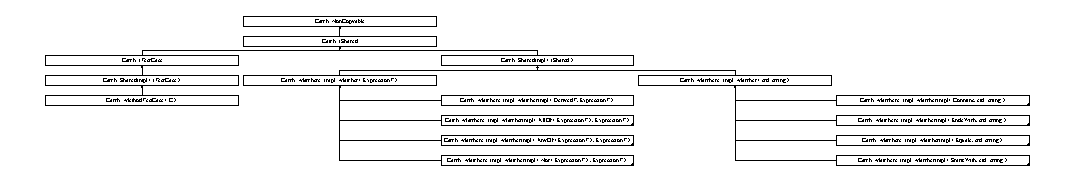
\includegraphics[height=2.004474cm]{struct_catch_1_1_i_shared}
\end{center}
\end{figure}
\subsection*{Public Member Functions}
\begin{DoxyCompactItemize}
\item 
\mbox{\Hypertarget{struct_catch_1_1_i_shared_ae383df68557cdaf0910b411af04d9e33}\label{struct_catch_1_1_i_shared_ae383df68557cdaf0910b411af04d9e33}} 
virtual void {\bfseries add\+Ref} () const =0
\item 
\mbox{\Hypertarget{struct_catch_1_1_i_shared_a002f52624728a763956fb6f230cb2f57}\label{struct_catch_1_1_i_shared_a002f52624728a763956fb6f230cb2f57}} 
virtual void {\bfseries release} () const =0
\end{DoxyCompactItemize}


\subsection{Detailed Description}


Definition at line 502 of file catch.\+hpp.



The documentation for this struct was generated from the following file\+:\begin{DoxyCompactItemize}
\item 
Tests/catch.\+hpp\end{DoxyCompactItemize}

\hypertarget{struct_catch_1_1_detail_1_1_is_stream_insertable}{}\section{Catch\+:\+:Detail\+:\+:Is\+Stream\+Insertable$<$ T $>$ Struct Template Reference}
\label{struct_catch_1_1_detail_1_1_is_stream_insertable}\index{Catch\+::\+Detail\+::\+Is\+Stream\+Insertable$<$ T $>$@{Catch\+::\+Detail\+::\+Is\+Stream\+Insertable$<$ T $>$}}
\subsection*{Public Types}
\begin{DoxyCompactItemize}
\item 
\mbox{\Hypertarget{struct_catch_1_1_detail_1_1_is_stream_insertable_a2e4508694da3bf368ff67733a7970edd}\label{struct_catch_1_1_detail_1_1_is_stream_insertable_a2e4508694da3bf368ff67733a7970edd}} 
enum \{ {\bfseries value} = sizeof( test\+Streamable(s $<$$<$ t) ) == sizeof( True\+Type )
 \}
\end{DoxyCompactItemize}
\subsection*{Static Public Attributes}
\begin{DoxyCompactItemize}
\item 
\mbox{\Hypertarget{struct_catch_1_1_detail_1_1_is_stream_insertable_abe3d3c8e5d85665747faafffc9a96b00}\label{struct_catch_1_1_detail_1_1_is_stream_insertable_abe3d3c8e5d85665747faafffc9a96b00}} 
static \textbf{ std\+::ostream} \& {\bfseries s}
\item 
\mbox{\Hypertarget{struct_catch_1_1_detail_1_1_is_stream_insertable_a7d2a3da978b6736667a7b2f6d51f507f}\label{struct_catch_1_1_detail_1_1_is_stream_insertable_a7d2a3da978b6736667a7b2f6d51f507f}} 
static T const  \& {\bfseries t}
\end{DoxyCompactItemize}


\subsection{Detailed Description}
\subsubsection*{template$<$typename T$>$\newline
struct Catch\+::\+Detail\+::\+Is\+Stream\+Insertable$<$ T $>$}



Definition at line 1572 of file catch.\+hpp.



The documentation for this struct was generated from the following file\+:\begin{DoxyCompactItemize}
\item 
Tests/catch.\+hpp\end{DoxyCompactItemize}

\hypertarget{struct_catch_1_1_i_tag_alias_registry}{}\section{Catch\+:\+:I\+Tag\+Alias\+Registry Struct Reference}
\label{struct_catch_1_1_i_tag_alias_registry}\index{Catch\+::\+I\+Tag\+Alias\+Registry@{Catch\+::\+I\+Tag\+Alias\+Registry}}
\subsection*{Public Member Functions}
\begin{DoxyCompactItemize}
\item 
\mbox{\Hypertarget{struct_catch_1_1_i_tag_alias_registry_a7d2fba4d39cfcc62c2695fcde4f989c3}\label{struct_catch_1_1_i_tag_alias_registry_a7d2fba4d39cfcc62c2695fcde4f989c3}} 
virtual \hyperlink{class_catch_1_1_option}{Option}$<$ \hyperlink{struct_catch_1_1_tag_alias}{Tag\+Alias} $>$ {\bfseries find} (\textbf{ std\+::string} const \&alias) const =0
\item 
\mbox{\Hypertarget{struct_catch_1_1_i_tag_alias_registry_ae729a7532faf7466db1a157ce0395170}\label{struct_catch_1_1_i_tag_alias_registry_ae729a7532faf7466db1a157ce0395170}} 
virtual \textbf{ std\+::string} {\bfseries expand\+Aliases} (\textbf{ std\+::string} const \&unexpanded\+Test\+Spec) const =0
\end{DoxyCompactItemize}
\subsection*{Static Public Member Functions}
\begin{DoxyCompactItemize}
\item 
\mbox{\Hypertarget{struct_catch_1_1_i_tag_alias_registry_aa9d0f008f49473389c7abf6071f137a7}\label{struct_catch_1_1_i_tag_alias_registry_aa9d0f008f49473389c7abf6071f137a7}} 
static \hyperlink{struct_catch_1_1_i_tag_alias_registry}{I\+Tag\+Alias\+Registry} const  \& {\bfseries get} ()
\end{DoxyCompactItemize}


\subsection{Detailed Description}


Definition at line 2743 of file catch.\+hpp.



The documentation for this struct was generated from the following file\+:\begin{DoxyCompactItemize}
\item 
Tests/catch.\+hpp\end{DoxyCompactItemize}

\hypertarget{struct_catch_1_1_i_test_case}{}\section{Catch\+:\+:I\+Test\+Case Struct Reference}
\label{struct_catch_1_1_i_test_case}\index{Catch\+::\+I\+Test\+Case@{Catch\+::\+I\+Test\+Case}}
Inheritance diagram for Catch\+:\+:I\+Test\+Case\+:\begin{figure}[H]
\begin{center}
\leavevmode
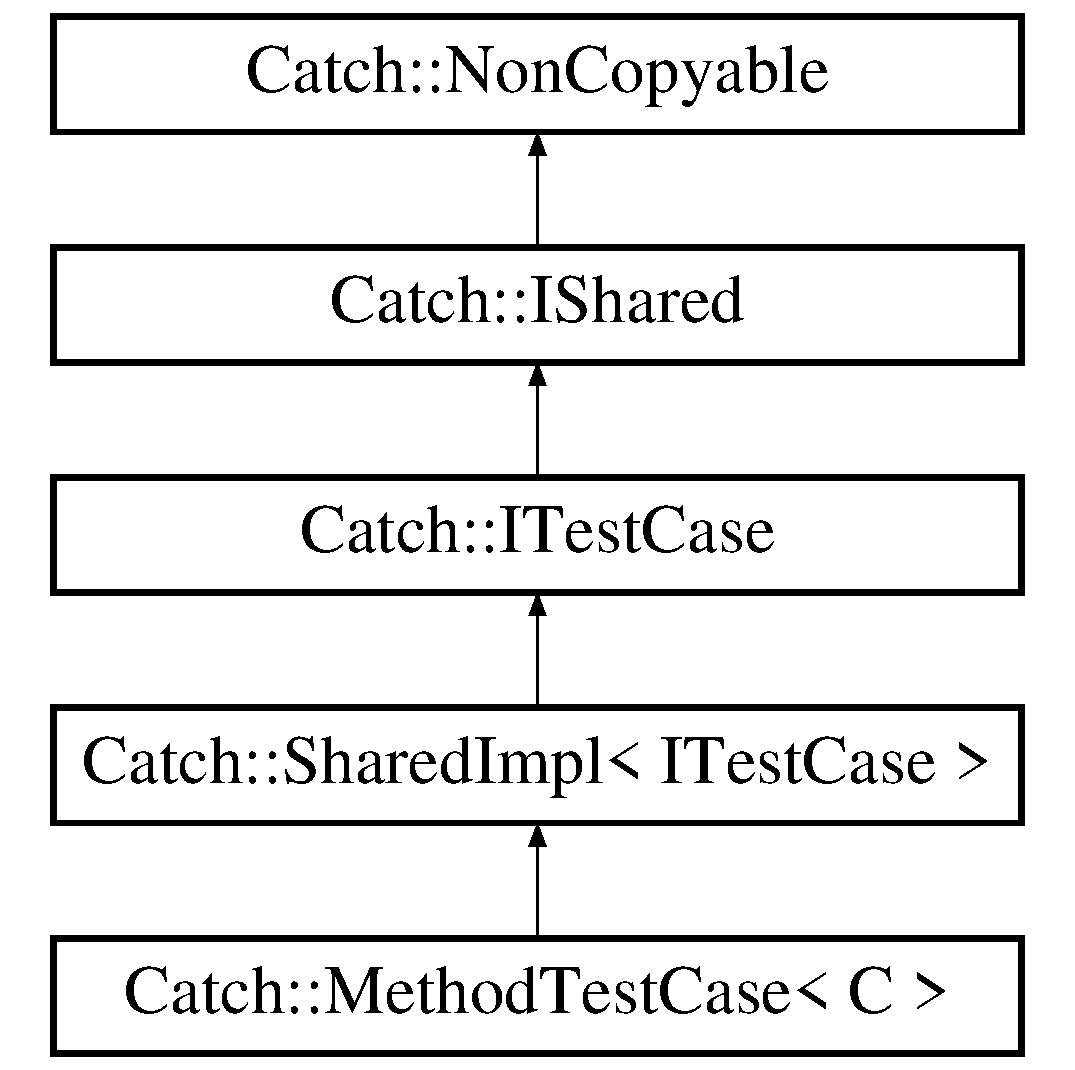
\includegraphics[height=5.000000cm]{struct_catch_1_1_i_test_case}
\end{center}
\end{figure}
\subsection*{Public Member Functions}
\begin{DoxyCompactItemize}
\item 
\mbox{\Hypertarget{struct_catch_1_1_i_test_case_a678825e62e7c17297621cfeb65588c34}\label{struct_catch_1_1_i_test_case_a678825e62e7c17297621cfeb65588c34}} 
virtual void {\bfseries invoke} () const =0
\end{DoxyCompactItemize}


\subsection{Detailed Description}


Definition at line 581 of file catch.\+hpp.



The documentation for this struct was generated from the following file\+:\begin{DoxyCompactItemize}
\item 
Tests/catch.\+hpp\end{DoxyCompactItemize}

\hypertarget{struct_catch_1_1_i_test_case_registry}{}\section{Catch\+:\+:I\+Test\+Case\+Registry Struct Reference}
\label{struct_catch_1_1_i_test_case_registry}\index{Catch\+::\+I\+Test\+Case\+Registry@{Catch\+::\+I\+Test\+Case\+Registry}}
\subsection*{Public Member Functions}
\begin{DoxyCompactItemize}
\item 
\mbox{\Hypertarget{struct_catch_1_1_i_test_case_registry_ad6e4d4a621655123f73ae98cfeda063d}\label{struct_catch_1_1_i_test_case_registry_ad6e4d4a621655123f73ae98cfeda063d}} 
virtual \textbf{ std\+::vector}$<$ \hyperlink{class_catch_1_1_test_case}{Test\+Case} $>$ const  \& {\bfseries get\+All\+Tests} () const =0
\item 
\mbox{\Hypertarget{struct_catch_1_1_i_test_case_registry_a33e46639d0319d35497c05bb5d02be5a}\label{struct_catch_1_1_i_test_case_registry_a33e46639d0319d35497c05bb5d02be5a}} 
virtual \textbf{ std\+::vector}$<$ \hyperlink{class_catch_1_1_test_case}{Test\+Case} $>$ const  \& {\bfseries get\+All\+Tests\+Sorted} (I\+Config const \&config) const =0
\end{DoxyCompactItemize}


\subsection{Detailed Description}


Definition at line 590 of file catch.\+hpp.



The documentation for this struct was generated from the following file\+:\begin{DoxyCompactItemize}
\item 
Tests/catch.\+hpp\end{DoxyCompactItemize}

\hypertarget{struct_catch_1_1_matchers_1_1_impl_1_1_matcher}{}\section{Catch\+:\+:Matchers\+:\+:Impl\+:\+:Matcher$<$ ExpressionT $>$ Struct Template Reference}
\label{struct_catch_1_1_matchers_1_1_impl_1_1_matcher}\index{Catch\+::\+Matchers\+::\+Impl\+::\+Matcher$<$ Expression\+T $>$@{Catch\+::\+Matchers\+::\+Impl\+::\+Matcher$<$ Expression\+T $>$}}
Inheritance diagram for Catch\+:\+:Matchers\+:\+:Impl\+:\+:Matcher$<$ ExpressionT $>$\+:\begin{figure}[H]
\begin{center}
\leavevmode
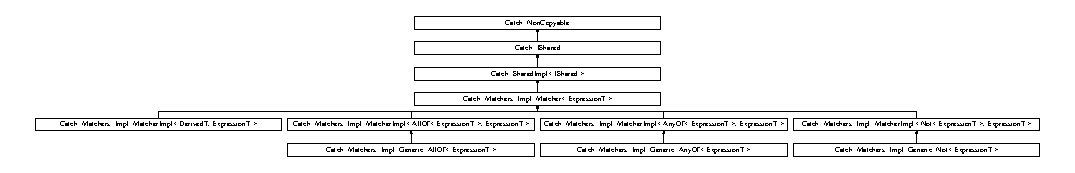
\includegraphics[height=1.879195cm]{struct_catch_1_1_matchers_1_1_impl_1_1_matcher}
\end{center}
\end{figure}
\subsection*{Public Types}
\begin{DoxyCompactItemize}
\item 
\mbox{\Hypertarget{struct_catch_1_1_matchers_1_1_impl_1_1_matcher_a7f5068cbacd1eed06cf243e63446e7e1}\label{struct_catch_1_1_matchers_1_1_impl_1_1_matcher_a7f5068cbacd1eed06cf243e63446e7e1}} 
typedef ExpressionT {\bfseries Expression\+Type}
\end{DoxyCompactItemize}
\subsection*{Public Member Functions}
\begin{DoxyCompactItemize}
\item 
\mbox{\Hypertarget{struct_catch_1_1_matchers_1_1_impl_1_1_matcher_a9d31e5018fea24efa08c3cbf5aa4475d}\label{struct_catch_1_1_matchers_1_1_impl_1_1_matcher_a9d31e5018fea24efa08c3cbf5aa4475d}} 
virtual \hyperlink{class_catch_1_1_ptr}{Ptr}$<$ \hyperlink{struct_catch_1_1_matchers_1_1_impl_1_1_matcher}{Matcher} $>$ {\bfseries clone} () const =0
\item 
\mbox{\Hypertarget{struct_catch_1_1_matchers_1_1_impl_1_1_matcher_a8c1c5511ce1f3738a45e6901b558f583}\label{struct_catch_1_1_matchers_1_1_impl_1_1_matcher_a8c1c5511ce1f3738a45e6901b558f583}} 
virtual bool {\bfseries match} (ExpressionT const \&expr) const =0
\item 
\mbox{\Hypertarget{struct_catch_1_1_matchers_1_1_impl_1_1_matcher_a091bcc37e589967d7e10fc7790d820e2}\label{struct_catch_1_1_matchers_1_1_impl_1_1_matcher_a091bcc37e589967d7e10fc7790d820e2}} 
virtual \textbf{ std\+::string} {\bfseries to\+String} () const =0
\item 
\mbox{\Hypertarget{struct_catch_1_1_matchers_1_1_impl_1_1_matcher_adb060f348e3ed404b80209fbc62174e1}\label{struct_catch_1_1_matchers_1_1_impl_1_1_matcher_adb060f348e3ed404b80209fbc62174e1}} 
\hyperlink{class_catch_1_1_matchers_1_1_impl_1_1_generic_1_1_all_of}{Generic\+::\+All\+Of}$<$ ExpressionT $>$ {\bfseries operator\&\&} (\hyperlink{struct_catch_1_1_matchers_1_1_impl_1_1_matcher}{Matcher}$<$ ExpressionT $>$ const \&other) const
\item 
\mbox{\Hypertarget{struct_catch_1_1_matchers_1_1_impl_1_1_matcher_a55b1e12315e7a5daf7ce7a11ddfaa295}\label{struct_catch_1_1_matchers_1_1_impl_1_1_matcher_a55b1e12315e7a5daf7ce7a11ddfaa295}} 
\hyperlink{class_catch_1_1_matchers_1_1_impl_1_1_generic_1_1_any_of}{Generic\+::\+Any\+Of}$<$ ExpressionT $>$ {\bfseries operator$\vert$$\vert$} (\hyperlink{struct_catch_1_1_matchers_1_1_impl_1_1_matcher}{Matcher}$<$ ExpressionT $>$ const \&other) const
\item 
\mbox{\Hypertarget{struct_catch_1_1_matchers_1_1_impl_1_1_matcher_a7ecd56842090611c9dbfc325b42fa942}\label{struct_catch_1_1_matchers_1_1_impl_1_1_matcher_a7ecd56842090611c9dbfc325b42fa942}} 
\hyperlink{class_catch_1_1_matchers_1_1_impl_1_1_generic_1_1_not}{Generic\+::\+Not}$<$ ExpressionT $>$ {\bfseries operator!} () const
\end{DoxyCompactItemize}
\subsection*{Additional Inherited Members}


\subsection{Detailed Description}
\subsubsection*{template$<$typename ExpressionT$>$\newline
struct Catch\+::\+Matchers\+::\+Impl\+::\+Matcher$<$ Expression\+T $>$}



Definition at line 858 of file catch.\+hpp.



The documentation for this struct was generated from the following file\+:\begin{DoxyCompactItemize}
\item 
Tests/catch.\+hpp\end{DoxyCompactItemize}

\hypertarget{struct_catch_1_1_matchers_1_1_impl_1_1_matcher_impl}{}\section{Catch\+:\+:Matchers\+:\+:Impl\+:\+:Matcher\+Impl$<$ DerivedT, ExpressionT $>$ Struct Template Reference}
\label{struct_catch_1_1_matchers_1_1_impl_1_1_matcher_impl}\index{Catch\+::\+Matchers\+::\+Impl\+::\+Matcher\+Impl$<$ Derived\+T, Expression\+T $>$@{Catch\+::\+Matchers\+::\+Impl\+::\+Matcher\+Impl$<$ Derived\+T, Expression\+T $>$}}
Inheritance diagram for Catch\+:\+:Matchers\+:\+:Impl\+:\+:Matcher\+Impl$<$ DerivedT, ExpressionT $>$\+:\begin{figure}[H]
\begin{center}
\leavevmode
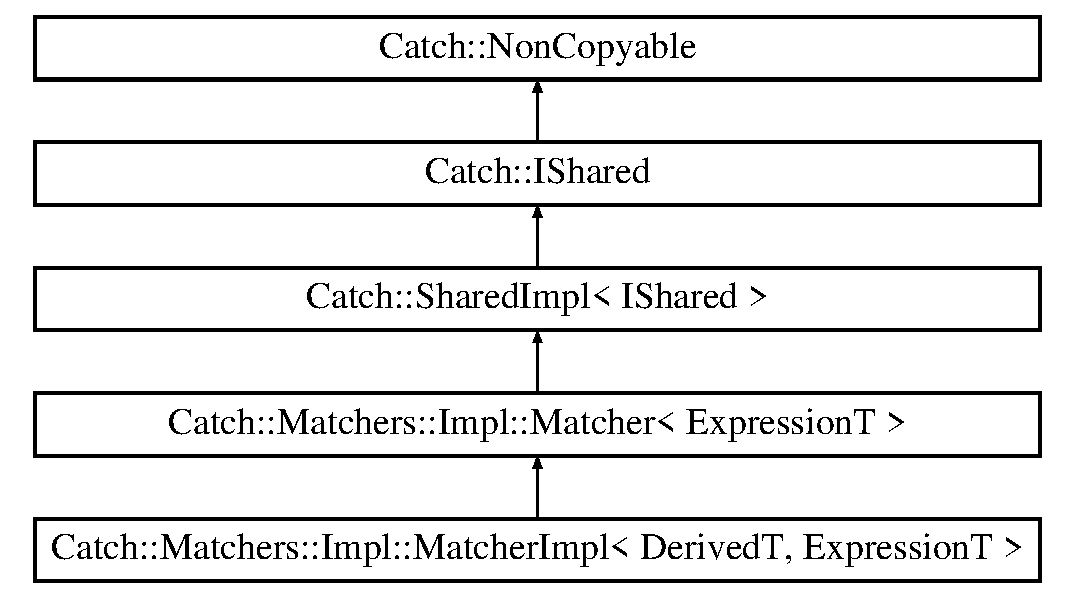
\includegraphics[height=5.000000cm]{struct_catch_1_1_matchers_1_1_impl_1_1_matcher_impl}
\end{center}
\end{figure}
\subsection*{Public Member Functions}
\begin{DoxyCompactItemize}
\item 
\mbox{\Hypertarget{struct_catch_1_1_matchers_1_1_impl_1_1_matcher_impl_af7cf4b7b730145d4455dc356490e6b77}\label{struct_catch_1_1_matchers_1_1_impl_1_1_matcher_impl_af7cf4b7b730145d4455dc356490e6b77}} 
virtual \hyperlink{class_catch_1_1_ptr}{Ptr}$<$ \hyperlink{struct_catch_1_1_matchers_1_1_impl_1_1_matcher}{Matcher}$<$ ExpressionT $>$ $>$ {\bfseries clone} () const
\end{DoxyCompactItemize}
\subsection*{Additional Inherited Members}


\subsection{Detailed Description}
\subsubsection*{template$<$typename DerivedT, typename ExpressionT$>$\newline
struct Catch\+::\+Matchers\+::\+Impl\+::\+Matcher\+Impl$<$ Derived\+T, Expression\+T $>$}



Definition at line 873 of file catch.\+hpp.



The documentation for this struct was generated from the following file\+:\begin{DoxyCompactItemize}
\item 
Tests/catch.\+hpp\end{DoxyCompactItemize}

\hypertarget{struct_catch_1_1_message_builder}{}\section{Catch\+:\+:Message\+Builder Struct Reference}
\label{struct_catch_1_1_message_builder}\index{Catch\+::\+Message\+Builder@{Catch\+::\+Message\+Builder}}
\subsection*{Public Member Functions}
\begin{DoxyCompactItemize}
\item 
\mbox{\Hypertarget{struct_catch_1_1_message_builder_ab0c6378e722680bf58852c6ee2b6e724}\label{struct_catch_1_1_message_builder_ab0c6378e722680bf58852c6ee2b6e724}} 
{\bfseries Message\+Builder} (\textbf{ std\+::string} const \&macro\+Name, \hyperlink{struct_catch_1_1_source_line_info}{Source\+Line\+Info} const \&line\+Info, Result\+Was\+::\+Of\+Type type)
\item 
\mbox{\Hypertarget{struct_catch_1_1_message_builder_a20fa48d069b20dddcc2d3df8abb123c1}\label{struct_catch_1_1_message_builder_a20fa48d069b20dddcc2d3df8abb123c1}} 
{\footnotesize template$<$typename T $>$ }\\\hyperlink{struct_catch_1_1_message_builder}{Message\+Builder} \& {\bfseries operator$<$$<$} (T const \&value)
\end{DoxyCompactItemize}
\subsection*{Public Attributes}
\begin{DoxyCompactItemize}
\item 
\mbox{\Hypertarget{struct_catch_1_1_message_builder_a979f1c2b36d78f80ee275bfa5ba0209f}\label{struct_catch_1_1_message_builder_a979f1c2b36d78f80ee275bfa5ba0209f}} 
\hyperlink{struct_catch_1_1_message_info}{Message\+Info} {\bfseries m\+\_\+info}
\item 
\mbox{\Hypertarget{struct_catch_1_1_message_builder_a6488ab0cc4ea52affc9c0612c7c5df6b}\label{struct_catch_1_1_message_builder_a6488ab0cc4ea52affc9c0612c7c5df6b}} 
\textbf{ std\+::ostringstream} {\bfseries m\+\_\+stream}
\end{DoxyCompactItemize}


\subsection{Detailed Description}


Definition at line 1883 of file catch.\+hpp.



The documentation for this struct was generated from the following file\+:\begin{DoxyCompactItemize}
\item 
Tests/catch.\+hpp\end{DoxyCompactItemize}

\hypertarget{struct_catch_1_1_message_info}{}\section{Catch\+:\+:Message\+Info Struct Reference}
\label{struct_catch_1_1_message_info}\index{Catch\+::\+Message\+Info@{Catch\+::\+Message\+Info}}
\subsection*{Public Member Functions}
\begin{DoxyCompactItemize}
\item 
\mbox{\Hypertarget{struct_catch_1_1_message_info_a2e336c33ebef7af3c1bbae6a56e14f8a}\label{struct_catch_1_1_message_info_a2e336c33ebef7af3c1bbae6a56e14f8a}} 
{\bfseries Message\+Info} (\textbf{ std\+::string} const \&\+\_\+macro\+Name, \hyperlink{struct_catch_1_1_source_line_info}{Source\+Line\+Info} const \&\+\_\+line\+Info, Result\+Was\+::\+Of\+Type \+\_\+type)
\item 
\mbox{\Hypertarget{struct_catch_1_1_message_info_af4b37f2172ba55395813b4bb6bbbde1a}\label{struct_catch_1_1_message_info_af4b37f2172ba55395813b4bb6bbbde1a}} 
bool {\bfseries operator==} (\hyperlink{struct_catch_1_1_message_info}{Message\+Info} const \&other) const
\item 
\mbox{\Hypertarget{struct_catch_1_1_message_info_a8254cb8fca2da02a29a9843cdcb79df1}\label{struct_catch_1_1_message_info_a8254cb8fca2da02a29a9843cdcb79df1}} 
bool {\bfseries operator$<$} (\hyperlink{struct_catch_1_1_message_info}{Message\+Info} const \&other) const
\end{DoxyCompactItemize}
\subsection*{Public Attributes}
\begin{DoxyCompactItemize}
\item 
\mbox{\Hypertarget{struct_catch_1_1_message_info_a156ade4b3cc731f6ec7b542ae47ba8e3}\label{struct_catch_1_1_message_info_a156ade4b3cc731f6ec7b542ae47ba8e3}} 
\textbf{ std\+::string} {\bfseries macro\+Name}
\item 
\mbox{\Hypertarget{struct_catch_1_1_message_info_a985165328723e599696ebd8e43195cc5}\label{struct_catch_1_1_message_info_a985165328723e599696ebd8e43195cc5}} 
\hyperlink{struct_catch_1_1_source_line_info}{Source\+Line\+Info} {\bfseries line\+Info}
\item 
\mbox{\Hypertarget{struct_catch_1_1_message_info_ae928b9117465c696e45951d9d0284e78}\label{struct_catch_1_1_message_info_ae928b9117465c696e45951d9d0284e78}} 
Result\+Was\+::\+Of\+Type {\bfseries type}
\item 
\mbox{\Hypertarget{struct_catch_1_1_message_info_ab6cd06e050bf426c6577502a5c50e256}\label{struct_catch_1_1_message_info_ab6cd06e050bf426c6577502a5c50e256}} 
\textbf{ std\+::string} {\bfseries message}
\item 
\mbox{\Hypertarget{struct_catch_1_1_message_info_a7f4f57ea21e50160adefce7b68a781d6}\label{struct_catch_1_1_message_info_a7f4f57ea21e50160adefce7b68a781d6}} 
unsigned int {\bfseries sequence}
\end{DoxyCompactItemize}


\subsection{Detailed Description}


Definition at line 1862 of file catch.\+hpp.



The documentation for this struct was generated from the following file\+:\begin{DoxyCompactItemize}
\item 
Tests/catch.\+hpp\end{DoxyCompactItemize}

\hypertarget{class_catch_1_1_method_test_case}{}\section{Catch\+:\+:Method\+Test\+Case$<$ C $>$ Class Template Reference}
\label{class_catch_1_1_method_test_case}\index{Catch\+::\+Method\+Test\+Case$<$ C $>$@{Catch\+::\+Method\+Test\+Case$<$ C $>$}}
Inheritance diagram for Catch\+:\+:Method\+Test\+Case$<$ C $>$\+:\begin{figure}[H]
\begin{center}
\leavevmode
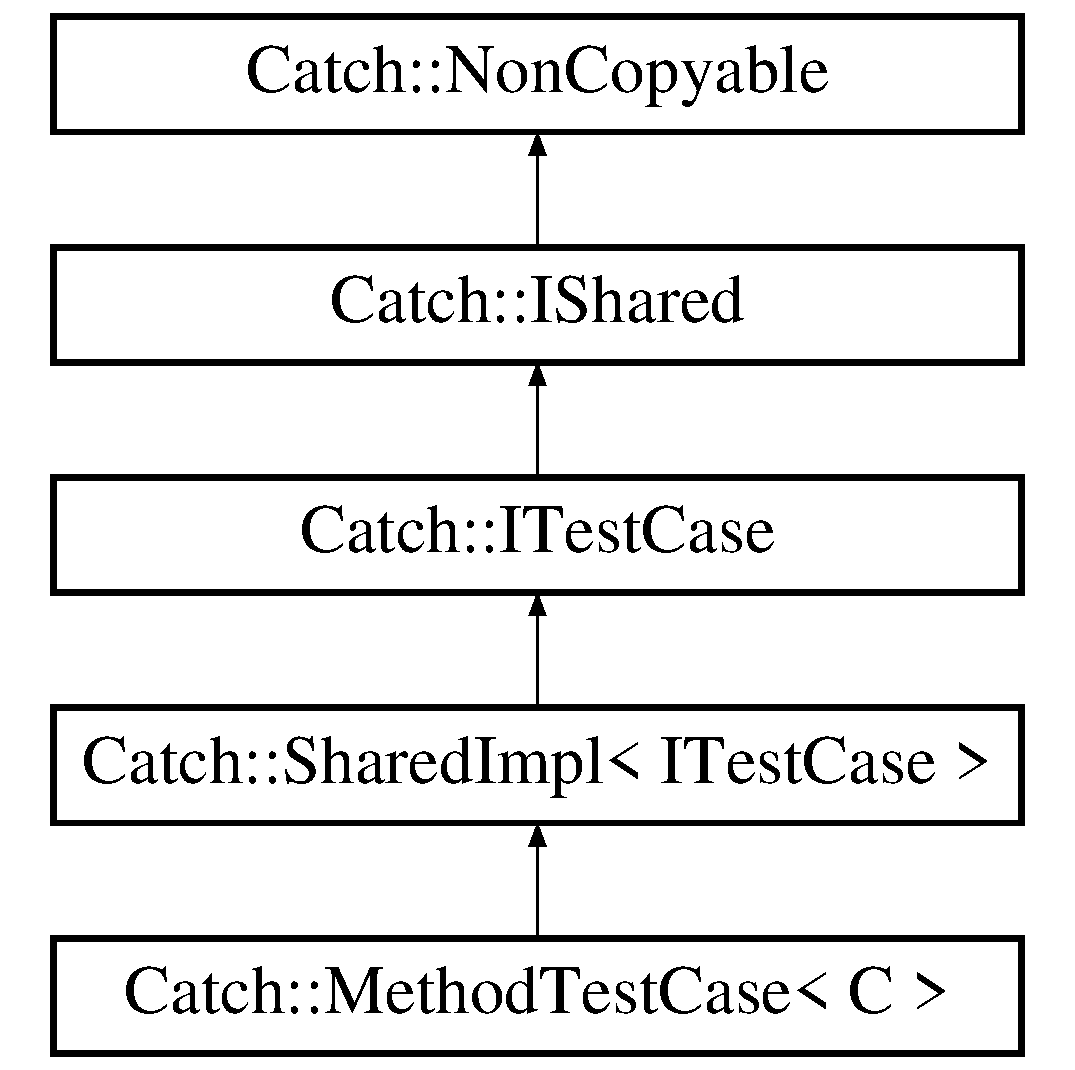
\includegraphics[height=5.000000cm]{class_catch_1_1_method_test_case}
\end{center}
\end{figure}
\subsection*{Public Member Functions}
\begin{DoxyCompactItemize}
\item 
\mbox{\Hypertarget{class_catch_1_1_method_test_case_a7b043b85dae371358255dd9dc6582e7b}\label{class_catch_1_1_method_test_case_a7b043b85dae371358255dd9dc6582e7b}} 
{\bfseries Method\+Test\+Case} (void(C\+::$\ast$method)())
\item 
\mbox{\Hypertarget{class_catch_1_1_method_test_case_a4e2263cfa0646f2980768328cb372793}\label{class_catch_1_1_method_test_case_a4e2263cfa0646f2980768328cb372793}} 
virtual void {\bfseries invoke} () const
\end{DoxyCompactItemize}
\subsection*{Additional Inherited Members}


\subsection{Detailed Description}
\subsubsection*{template$<$typename C$>$\newline
class Catch\+::\+Method\+Test\+Case$<$ C $>$}



Definition at line 605 of file catch.\+hpp.



The documentation for this class was generated from the following file\+:\begin{DoxyCompactItemize}
\item 
Tests/catch.\+hpp\end{DoxyCompactItemize}

\hypertarget{struct_catch_1_1_name_and_desc}{}\section{Catch\+:\+:Name\+And\+Desc Struct Reference}
\label{struct_catch_1_1_name_and_desc}\index{Catch\+::\+Name\+And\+Desc@{Catch\+::\+Name\+And\+Desc}}
\subsection*{Public Member Functions}
\begin{DoxyCompactItemize}
\item 
\mbox{\Hypertarget{struct_catch_1_1_name_and_desc_a189ceb9942fb5f6635140d6a09fc843a}\label{struct_catch_1_1_name_and_desc_a189ceb9942fb5f6635140d6a09fc843a}} 
{\bfseries Name\+And\+Desc} (const char $\ast$\+\_\+name=\char`\"{}\char`\"{}, const char $\ast$\+\_\+description=\char`\"{}\char`\"{})
\end{DoxyCompactItemize}
\subsection*{Public Attributes}
\begin{DoxyCompactItemize}
\item 
\mbox{\Hypertarget{struct_catch_1_1_name_and_desc_a374b4ed8be3cf98be20ebde5273bde51}\label{struct_catch_1_1_name_and_desc_a374b4ed8be3cf98be20ebde5273bde51}} 
const char $\ast$ {\bfseries name}
\item 
\mbox{\Hypertarget{struct_catch_1_1_name_and_desc_a3463a23ff65ce494fc380452b57b7970}\label{struct_catch_1_1_name_and_desc_a3463a23ff65ce494fc380452b57b7970}} 
const char $\ast$ {\bfseries description}
\end{DoxyCompactItemize}


\subsection{Detailed Description}


Definition at line 623 of file catch.\+hpp.



The documentation for this struct was generated from the following file\+:\begin{DoxyCompactItemize}
\item 
Tests/catch.\+hpp\end{DoxyCompactItemize}

\hypertarget{class_catch_1_1_non_copyable}{}\section{Catch\+:\+:Non\+Copyable Class Reference}
\label{class_catch_1_1_non_copyable}\index{Catch\+::\+Non\+Copyable@{Catch\+::\+Non\+Copyable}}
Inheritance diagram for Catch\+:\+:Non\+Copyable\+:\begin{figure}[H]
\begin{center}
\leavevmode
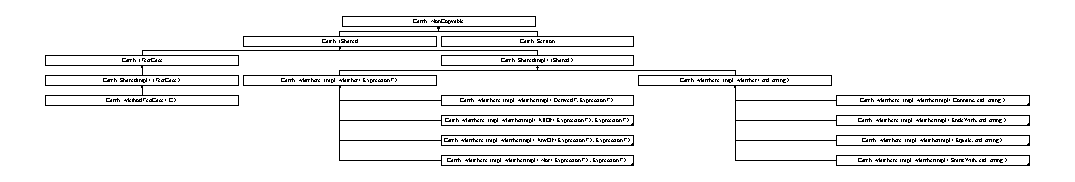
\includegraphics[height=2.004474cm]{class_catch_1_1_non_copyable}
\end{center}
\end{figure}


\subsection{Detailed Description}


Definition at line 289 of file catch.\+hpp.



The documentation for this class was generated from the following file\+:\begin{DoxyCompactItemize}
\item 
Tests/catch.\+hpp\end{DoxyCompactItemize}

\hypertarget{class_catch_1_1_matchers_1_1_impl_1_1_generic_1_1_not}{}\section{Catch\+:\+:Matchers\+:\+:Impl\+:\+:Generic\+:\+:Not$<$ ExpressionT $>$ Class Template Reference}
\label{class_catch_1_1_matchers_1_1_impl_1_1_generic_1_1_not}\index{Catch\+::\+Matchers\+::\+Impl\+::\+Generic\+::\+Not$<$ Expression\+T $>$@{Catch\+::\+Matchers\+::\+Impl\+::\+Generic\+::\+Not$<$ Expression\+T $>$}}
Inheritance diagram for Catch\+:\+:Matchers\+:\+:Impl\+:\+:Generic\+:\+:Not$<$ ExpressionT $>$\+:\begin{figure}[H]
\begin{center}
\leavevmode
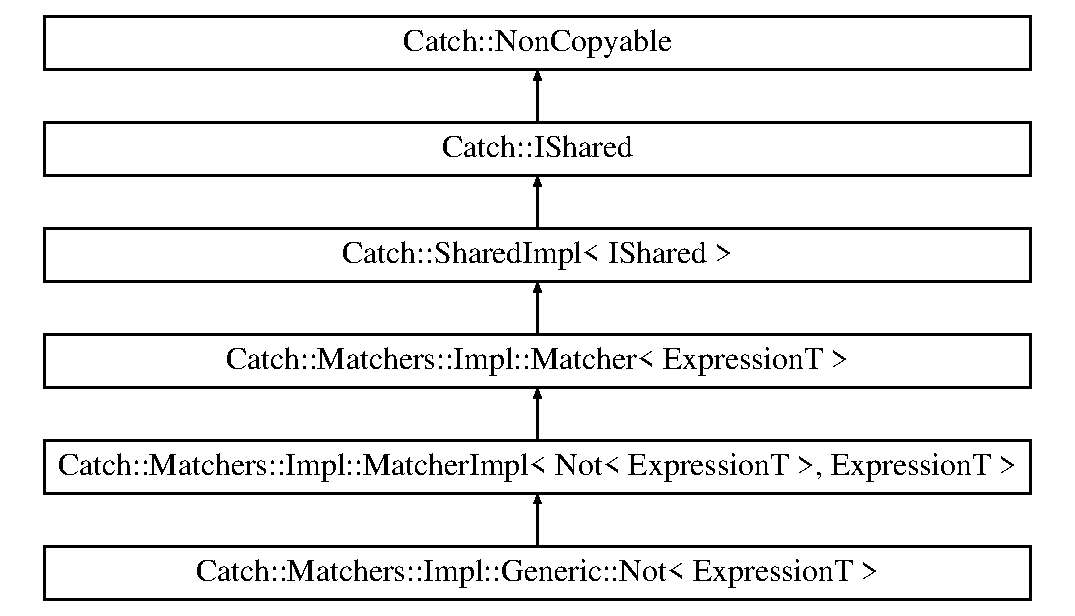
\includegraphics[height=6.000000cm]{class_catch_1_1_matchers_1_1_impl_1_1_generic_1_1_not}
\end{center}
\end{figure}
\subsection*{Public Member Functions}
\begin{DoxyCompactItemize}
\item 
\mbox{\Hypertarget{class_catch_1_1_matchers_1_1_impl_1_1_generic_1_1_not_a9b99e3ce49c1a16931708b67c312f204}\label{class_catch_1_1_matchers_1_1_impl_1_1_generic_1_1_not_a9b99e3ce49c1a16931708b67c312f204}} 
{\bfseries Not} (\hyperlink{struct_catch_1_1_matchers_1_1_impl_1_1_matcher}{Matcher}$<$ ExpressionT $>$ const \&matcher)
\item 
\mbox{\Hypertarget{class_catch_1_1_matchers_1_1_impl_1_1_generic_1_1_not_a46eccbbaeec259d3536aa2a29f95208f}\label{class_catch_1_1_matchers_1_1_impl_1_1_generic_1_1_not_a46eccbbaeec259d3536aa2a29f95208f}} 
{\bfseries Not} (\hyperlink{class_catch_1_1_matchers_1_1_impl_1_1_generic_1_1_not}{Not} const \&other)
\item 
\mbox{\Hypertarget{class_catch_1_1_matchers_1_1_impl_1_1_generic_1_1_not_a18c49fc6fb73a42d54650dafc18c7db1}\label{class_catch_1_1_matchers_1_1_impl_1_1_generic_1_1_not_a18c49fc6fb73a42d54650dafc18c7db1}} 
virtual bool {\bfseries match} (ExpressionT const \&expr) const C\+A\+T\+C\+H\+\_\+\+O\+V\+E\+R\+R\+I\+DE
\item 
\mbox{\Hypertarget{class_catch_1_1_matchers_1_1_impl_1_1_generic_1_1_not_ab970a4a6e58a987451e0b0e0e60a0bff}\label{class_catch_1_1_matchers_1_1_impl_1_1_generic_1_1_not_ab970a4a6e58a987451e0b0e0e60a0bff}} 
virtual \textbf{ std\+::string} {\bfseries to\+String} () const C\+A\+T\+C\+H\+\_\+\+O\+V\+E\+R\+R\+I\+DE
\end{DoxyCompactItemize}
\subsection*{Additional Inherited Members}


\subsection{Detailed Description}
\subsubsection*{template$<$typename ExpressionT$>$\newline
class Catch\+::\+Matchers\+::\+Impl\+::\+Generic\+::\+Not$<$ Expression\+T $>$}



Definition at line 854 of file catch.\+hpp.



The documentation for this class was generated from the following file\+:\begin{DoxyCompactItemize}
\item 
Tests/catch.\+hpp\end{DoxyCompactItemize}

\hypertarget{class_catch_1_1_not_implemented_exception}{}\section{Catch\+:\+:Not\+Implemented\+Exception Class Reference}
\label{class_catch_1_1_not_implemented_exception}\index{Catch\+::\+Not\+Implemented\+Exception@{Catch\+::\+Not\+Implemented\+Exception}}
Inheritance diagram for Catch\+:\+:Not\+Implemented\+Exception\+:\begin{figure}[H]
\begin{center}
\leavevmode
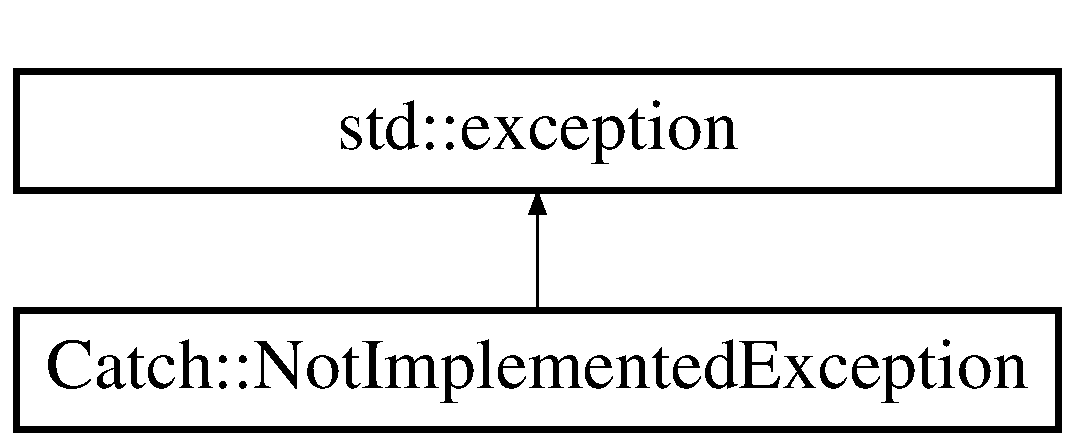
\includegraphics[height=2.000000cm]{class_catch_1_1_not_implemented_exception}
\end{center}
\end{figure}
\subsection*{Public Member Functions}
\begin{DoxyCompactItemize}
\item 
\mbox{\Hypertarget{class_catch_1_1_not_implemented_exception_ab4f0a5c39d8ffb72c664e2c07e180634}\label{class_catch_1_1_not_implemented_exception_ab4f0a5c39d8ffb72c664e2c07e180634}} 
{\bfseries Not\+Implemented\+Exception} (\hyperlink{struct_catch_1_1_source_line_info}{Source\+Line\+Info} const \&line\+Info)
\item 
\mbox{\Hypertarget{class_catch_1_1_not_implemented_exception_a508a7a833455da2d3c10ea1a9d45e982}\label{class_catch_1_1_not_implemented_exception_a508a7a833455da2d3c10ea1a9d45e982}} 
{\bfseries Not\+Implemented\+Exception} (\hyperlink{class_catch_1_1_not_implemented_exception}{Not\+Implemented\+Exception} const \&)
\item 
\mbox{\Hypertarget{class_catch_1_1_not_implemented_exception_ad4c13963f1a8feacda0cd331adda89e3}\label{class_catch_1_1_not_implemented_exception_ad4c13963f1a8feacda0cd331adda89e3}} 
virtual const char $\ast$ {\bfseries what} () const C\+A\+T\+C\+H\+\_\+\+N\+O\+E\+X\+C\+E\+PT
\end{DoxyCompactItemize}


\subsection{Detailed Description}


Definition at line 400 of file catch.\+hpp.



The documentation for this class was generated from the following file\+:\begin{DoxyCompactItemize}
\item 
Tests/catch.\+hpp\end{DoxyCompactItemize}

\hypertarget{struct_catch_1_1_internal_1_1_operator_traits}{}\section{Catch\+:\+:Internal\+:\+:Operator\+Traits$<$ Op $>$ Struct Template Reference}
\label{struct_catch_1_1_internal_1_1_operator_traits}\index{Catch\+::\+Internal\+::\+Operator\+Traits$<$ Op $>$@{Catch\+::\+Internal\+::\+Operator\+Traits$<$ Op $>$}}
\subsection*{Static Public Member Functions}
\begin{DoxyCompactItemize}
\item 
\mbox{\Hypertarget{struct_catch_1_1_internal_1_1_operator_traits_ac6d08082ea33348d42bc4ccbd6d07671}\label{struct_catch_1_1_internal_1_1_operator_traits_ac6d08082ea33348d42bc4ccbd6d07671}} 
static const char $\ast$ {\bfseries get\+Name} ()
\end{DoxyCompactItemize}


\subsection{Detailed Description}
\subsubsection*{template$<$Operator Op$>$\newline
struct Catch\+::\+Internal\+::\+Operator\+Traits$<$ Op $>$}



Definition at line 1266 of file catch.\+hpp.



The documentation for this struct was generated from the following file\+:\begin{DoxyCompactItemize}
\item 
Tests/catch.\+hpp\end{DoxyCompactItemize}

\hypertarget{struct_catch_1_1_internal_1_1_operator_traits_3_01_is_equal_to_01_4}{}\section{Catch\+:\+:Internal\+:\+:Operator\+Traits$<$ Is\+Equal\+To $>$ Struct Template Reference}
\label{struct_catch_1_1_internal_1_1_operator_traits_3_01_is_equal_to_01_4}\index{Catch\+::\+Internal\+::\+Operator\+Traits$<$ Is\+Equal\+To $>$@{Catch\+::\+Internal\+::\+Operator\+Traits$<$ Is\+Equal\+To $>$}}
\subsection*{Static Public Member Functions}
\begin{DoxyCompactItemize}
\item 
\mbox{\Hypertarget{struct_catch_1_1_internal_1_1_operator_traits_3_01_is_equal_to_01_4_addf03ac66f0ed83abcc037a7a327d4f1}\label{struct_catch_1_1_internal_1_1_operator_traits_3_01_is_equal_to_01_4_addf03ac66f0ed83abcc037a7a327d4f1}} 
static const char $\ast$ {\bfseries get\+Name} ()
\end{DoxyCompactItemize}


\subsection{Detailed Description}
\subsubsection*{template$<$$>$\newline
struct Catch\+::\+Internal\+::\+Operator\+Traits$<$ Is\+Equal\+To $>$}



Definition at line 1267 of file catch.\+hpp.



The documentation for this struct was generated from the following file\+:\begin{DoxyCompactItemize}
\item 
Tests/catch.\+hpp\end{DoxyCompactItemize}

\hypertarget{struct_catch_1_1_internal_1_1_operator_traits_3_01_is_greater_than_01_4}{}\section{Catch\+:\+:Internal\+:\+:Operator\+Traits$<$ Is\+Greater\+Than $>$ Struct Template Reference}
\label{struct_catch_1_1_internal_1_1_operator_traits_3_01_is_greater_than_01_4}\index{Catch\+::\+Internal\+::\+Operator\+Traits$<$ Is\+Greater\+Than $>$@{Catch\+::\+Internal\+::\+Operator\+Traits$<$ Is\+Greater\+Than $>$}}
\subsection*{Static Public Member Functions}
\begin{DoxyCompactItemize}
\item 
\mbox{\Hypertarget{struct_catch_1_1_internal_1_1_operator_traits_3_01_is_greater_than_01_4_ab917bfb9ccbe461dc684ee5a34d67d27}\label{struct_catch_1_1_internal_1_1_operator_traits_3_01_is_greater_than_01_4_ab917bfb9ccbe461dc684ee5a34d67d27}} 
static const char $\ast$ {\bfseries get\+Name} ()
\end{DoxyCompactItemize}


\subsection{Detailed Description}
\subsubsection*{template$<$$>$\newline
struct Catch\+::\+Internal\+::\+Operator\+Traits$<$ Is\+Greater\+Than $>$}



Definition at line 1270 of file catch.\+hpp.



The documentation for this struct was generated from the following file\+:\begin{DoxyCompactItemize}
\item 
Tests/catch.\+hpp\end{DoxyCompactItemize}

\hypertarget{struct_catch_1_1_internal_1_1_operator_traits_3_01_is_greater_than_or_equal_to_01_4}{}\section{Catch\+:\+:Internal\+:\+:Operator\+Traits$<$ Is\+Greater\+Than\+Or\+Equal\+To $>$ Struct Template Reference}
\label{struct_catch_1_1_internal_1_1_operator_traits_3_01_is_greater_than_or_equal_to_01_4}\index{Catch\+::\+Internal\+::\+Operator\+Traits$<$ Is\+Greater\+Than\+Or\+Equal\+To $>$@{Catch\+::\+Internal\+::\+Operator\+Traits$<$ Is\+Greater\+Than\+Or\+Equal\+To $>$}}
\subsection*{Static Public Member Functions}
\begin{DoxyCompactItemize}
\item 
\mbox{\Hypertarget{struct_catch_1_1_internal_1_1_operator_traits_3_01_is_greater_than_or_equal_to_01_4_a76b6f6b0dbaf7d19ebb1b4b4891e719e}\label{struct_catch_1_1_internal_1_1_operator_traits_3_01_is_greater_than_or_equal_to_01_4_a76b6f6b0dbaf7d19ebb1b4b4891e719e}} 
static const char $\ast$ {\bfseries get\+Name} ()
\end{DoxyCompactItemize}


\subsection{Detailed Description}
\subsubsection*{template$<$$>$\newline
struct Catch\+::\+Internal\+::\+Operator\+Traits$<$ Is\+Greater\+Than\+Or\+Equal\+To $>$}



Definition at line 1272 of file catch.\+hpp.



The documentation for this struct was generated from the following file\+:\begin{DoxyCompactItemize}
\item 
Tests/catch.\+hpp\end{DoxyCompactItemize}

\hypertarget{struct_catch_1_1_internal_1_1_operator_traits_3_01_is_less_than_01_4}{}\section{Catch\+:\+:Internal\+:\+:Operator\+Traits$<$ Is\+Less\+Than $>$ Struct Template Reference}
\label{struct_catch_1_1_internal_1_1_operator_traits_3_01_is_less_than_01_4}\index{Catch\+::\+Internal\+::\+Operator\+Traits$<$ Is\+Less\+Than $>$@{Catch\+::\+Internal\+::\+Operator\+Traits$<$ Is\+Less\+Than $>$}}
\subsection*{Static Public Member Functions}
\begin{DoxyCompactItemize}
\item 
\mbox{\Hypertarget{struct_catch_1_1_internal_1_1_operator_traits_3_01_is_less_than_01_4_aa3b536ddbd2e34b1253931ff00c32712}\label{struct_catch_1_1_internal_1_1_operator_traits_3_01_is_less_than_01_4_aa3b536ddbd2e34b1253931ff00c32712}} 
static const char $\ast$ {\bfseries get\+Name} ()
\end{DoxyCompactItemize}


\subsection{Detailed Description}
\subsubsection*{template$<$$>$\newline
struct Catch\+::\+Internal\+::\+Operator\+Traits$<$ Is\+Less\+Than $>$}



Definition at line 1269 of file catch.\+hpp.



The documentation for this struct was generated from the following file\+:\begin{DoxyCompactItemize}
\item 
Tests/catch.\+hpp\end{DoxyCompactItemize}

\hypertarget{struct_catch_1_1_internal_1_1_operator_traits_3_01_is_less_than_or_equal_to_01_4}{}\section{Catch\+:\+:Internal\+:\+:Operator\+Traits$<$ Is\+Less\+Than\+Or\+Equal\+To $>$ Struct Template Reference}
\label{struct_catch_1_1_internal_1_1_operator_traits_3_01_is_less_than_or_equal_to_01_4}\index{Catch\+::\+Internal\+::\+Operator\+Traits$<$ Is\+Less\+Than\+Or\+Equal\+To $>$@{Catch\+::\+Internal\+::\+Operator\+Traits$<$ Is\+Less\+Than\+Or\+Equal\+To $>$}}
\subsection*{Static Public Member Functions}
\begin{DoxyCompactItemize}
\item 
\mbox{\Hypertarget{struct_catch_1_1_internal_1_1_operator_traits_3_01_is_less_than_or_equal_to_01_4_ae8578813bc847838f10448c1541a9d7b}\label{struct_catch_1_1_internal_1_1_operator_traits_3_01_is_less_than_or_equal_to_01_4_ae8578813bc847838f10448c1541a9d7b}} 
static const char $\ast$ {\bfseries get\+Name} ()
\end{DoxyCompactItemize}


\subsection{Detailed Description}
\subsubsection*{template$<$$>$\newline
struct Catch\+::\+Internal\+::\+Operator\+Traits$<$ Is\+Less\+Than\+Or\+Equal\+To $>$}



Definition at line 1271 of file catch.\+hpp.



The documentation for this struct was generated from the following file\+:\begin{DoxyCompactItemize}
\item 
Tests/catch.\+hpp\end{DoxyCompactItemize}

\hypertarget{struct_catch_1_1_internal_1_1_operator_traits_3_01_is_not_equal_to_01_4}{}\section{Catch\+:\+:Internal\+:\+:Operator\+Traits$<$ Is\+Not\+Equal\+To $>$ Struct Template Reference}
\label{struct_catch_1_1_internal_1_1_operator_traits_3_01_is_not_equal_to_01_4}\index{Catch\+::\+Internal\+::\+Operator\+Traits$<$ Is\+Not\+Equal\+To $>$@{Catch\+::\+Internal\+::\+Operator\+Traits$<$ Is\+Not\+Equal\+To $>$}}
\subsection*{Static Public Member Functions}
\begin{DoxyCompactItemize}
\item 
\mbox{\Hypertarget{struct_catch_1_1_internal_1_1_operator_traits_3_01_is_not_equal_to_01_4_a54a795b8bf7c80a9fdbc7b81f39133b4}\label{struct_catch_1_1_internal_1_1_operator_traits_3_01_is_not_equal_to_01_4_a54a795b8bf7c80a9fdbc7b81f39133b4}} 
static const char $\ast$ {\bfseries get\+Name} ()
\end{DoxyCompactItemize}


\subsection{Detailed Description}
\subsubsection*{template$<$$>$\newline
struct Catch\+::\+Internal\+::\+Operator\+Traits$<$ Is\+Not\+Equal\+To $>$}



Definition at line 1268 of file catch.\+hpp.



The documentation for this struct was generated from the following file\+:\begin{DoxyCompactItemize}
\item 
Tests/catch.\+hpp\end{DoxyCompactItemize}

\hypertarget{class_catch_1_1_option}{}\section{Catch\+:\+:Option$<$ T $>$ Class Template Reference}
\label{class_catch_1_1_option}\index{Catch\+::\+Option$<$ T $>$@{Catch\+::\+Option$<$ T $>$}}
\subsection*{Public Member Functions}
\begin{DoxyCompactItemize}
\item 
\mbox{\Hypertarget{class_catch_1_1_option_a5aeb9c22d48a6882bdf5fb4730b06c86}\label{class_catch_1_1_option_a5aeb9c22d48a6882bdf5fb4730b06c86}} 
{\bfseries Option} (T const \&\+\_\+value)
\item 
\mbox{\Hypertarget{class_catch_1_1_option_af02f2e4559f06384baec0def8c68c5fd}\label{class_catch_1_1_option_af02f2e4559f06384baec0def8c68c5fd}} 
{\bfseries Option} (\hyperlink{class_catch_1_1_option}{Option} const \&\+\_\+other)
\item 
\mbox{\Hypertarget{class_catch_1_1_option_a78c65b15dd6b2fbd04c5012c43017c8f}\label{class_catch_1_1_option_a78c65b15dd6b2fbd04c5012c43017c8f}} 
\hyperlink{class_catch_1_1_option}{Option} \& {\bfseries operator=} (\hyperlink{class_catch_1_1_option}{Option} const \&\+\_\+other)
\item 
\mbox{\Hypertarget{class_catch_1_1_option_a2be7e343ab22d6061726d32ab4622653}\label{class_catch_1_1_option_a2be7e343ab22d6061726d32ab4622653}} 
\hyperlink{class_catch_1_1_option}{Option} \& {\bfseries operator=} (T const \&\+\_\+value)
\item 
\mbox{\Hypertarget{class_catch_1_1_option_a37b4e0e5d4d56296adacd267a616f4e0}\label{class_catch_1_1_option_a37b4e0e5d4d56296adacd267a616f4e0}} 
void {\bfseries reset} ()
\item 
\mbox{\Hypertarget{class_catch_1_1_option_afd989852fa453731c3190dac63caccb0}\label{class_catch_1_1_option_afd989852fa453731c3190dac63caccb0}} 
T \& {\bfseries operator$\ast$} ()
\item 
\mbox{\Hypertarget{class_catch_1_1_option_a734fc9c2eb1a1f7f8e8f6a4eb12160f0}\label{class_catch_1_1_option_a734fc9c2eb1a1f7f8e8f6a4eb12160f0}} 
T const  \& {\bfseries operator$\ast$} () const
\item 
\mbox{\Hypertarget{class_catch_1_1_option_acad340798a16c8f700f8763119e90f31}\label{class_catch_1_1_option_acad340798a16c8f700f8763119e90f31}} 
T $\ast$ {\bfseries operator-\/$>$} ()
\item 
\mbox{\Hypertarget{class_catch_1_1_option_ae8343cbc36dbb95b2dce333d2a6fdc28}\label{class_catch_1_1_option_ae8343cbc36dbb95b2dce333d2a6fdc28}} 
const T $\ast$ {\bfseries operator-\/$>$} () const
\item 
\mbox{\Hypertarget{class_catch_1_1_option_a8d9ae2e30b0eb76fe134a6fbc8423124}\label{class_catch_1_1_option_a8d9ae2e30b0eb76fe134a6fbc8423124}} 
T {\bfseries value\+Or} (T const \&default\+Value) const
\item 
\mbox{\Hypertarget{class_catch_1_1_option_a97c95829afbe92f2bcc5fd75b32c0825}\label{class_catch_1_1_option_a97c95829afbe92f2bcc5fd75b32c0825}} 
bool {\bfseries some} () const
\item 
\mbox{\Hypertarget{class_catch_1_1_option_a821753afdc3fac947a13a01fbe0d248e}\label{class_catch_1_1_option_a821753afdc3fac947a13a01fbe0d248e}} 
bool {\bfseries none} () const
\item 
\mbox{\Hypertarget{class_catch_1_1_option_a96dccb86bdf45ee0c08e122b6133bef3}\label{class_catch_1_1_option_a96dccb86bdf45ee0c08e122b6133bef3}} 
bool {\bfseries operator!} () const
\item 
\mbox{\Hypertarget{class_catch_1_1_option_a8ed8de7b072f893c85df14913dbbe197}\label{class_catch_1_1_option_a8ed8de7b072f893c85df14913dbbe197}} 
{\bfseries operator Safe\+Bool\+::type} () const
\end{DoxyCompactItemize}


\subsection{Detailed Description}
\subsubsection*{template$<$typename T$>$\newline
class Catch\+::\+Option$<$ T $>$}



Definition at line 2683 of file catch.\+hpp.



The documentation for this class was generated from the following file\+:\begin{DoxyCompactItemize}
\item 
Tests/catch.\+hpp\end{DoxyCompactItemize}

\hypertarget{struct_catch_1_1pluralise}{}\section{Catch\+:\+:pluralise Struct Reference}
\label{struct_catch_1_1pluralise}\index{Catch\+::pluralise@{Catch\+::pluralise}}
\subsection*{Public Member Functions}
\begin{DoxyCompactItemize}
\item 
\mbox{\Hypertarget{struct_catch_1_1pluralise_a5c55e22de2416cfe416edf715c6b9234}\label{struct_catch_1_1pluralise_a5c55e22de2416cfe416edf715c6b9234}} 
{\bfseries pluralise} (\textbf{ std\+::size\+\_\+t} count, \textbf{ std\+::string} const \&label)
\end{DoxyCompactItemize}
\subsection*{Public Attributes}
\begin{DoxyCompactItemize}
\item 
\mbox{\Hypertarget{struct_catch_1_1pluralise_a4dce2fa13ec6f00fac09b2418265441e}\label{struct_catch_1_1pluralise_a4dce2fa13ec6f00fac09b2418265441e}} 
\textbf{ std\+::size\+\_\+t} {\bfseries m\+\_\+count}
\item 
\mbox{\Hypertarget{struct_catch_1_1pluralise_a8849cbdd3f11ebe7747597c8644e8793}\label{struct_catch_1_1pluralise_a8849cbdd3f11ebe7747597c8644e8793}} 
\textbf{ std\+::string} {\bfseries m\+\_\+label}
\end{DoxyCompactItemize}
\subsection*{Friends}
\begin{DoxyCompactItemize}
\item 
\mbox{\Hypertarget{struct_catch_1_1pluralise_aa7dac6b165514c1f85e0695d678fdef5}\label{struct_catch_1_1pluralise_aa7dac6b165514c1f85e0695d678fdef5}} 
\textbf{ std\+::ostream} \& {\bfseries operator$<$$<$} (\textbf{ std\+::ostream} \&os, \hyperlink{struct_catch_1_1pluralise}{pluralise} const \&pluraliser)
\end{DoxyCompactItemize}


\subsection{Detailed Description}


Definition at line 339 of file catch.\+hpp.



The documentation for this struct was generated from the following file\+:\begin{DoxyCompactItemize}
\item 
Tests/catch.\+hpp\end{DoxyCompactItemize}

\hypertarget{class_catch_1_1_ptr}{}\section{Catch\+:\+:Ptr$<$ T $>$ Class Template Reference}
\label{class_catch_1_1_ptr}\index{Catch\+::\+Ptr$<$ T $>$@{Catch\+::\+Ptr$<$ T $>$}}
\subsection*{Public Member Functions}
\begin{DoxyCompactItemize}
\item 
\mbox{\Hypertarget{class_catch_1_1_ptr_aacec063a79cd142e39040a31c6b3c40b}\label{class_catch_1_1_ptr_aacec063a79cd142e39040a31c6b3c40b}} 
{\bfseries Ptr} (T $\ast$p)
\item 
\mbox{\Hypertarget{class_catch_1_1_ptr_ac629dd8ebe5763a37bb89e6c1d6a1771}\label{class_catch_1_1_ptr_ac629dd8ebe5763a37bb89e6c1d6a1771}} 
{\bfseries Ptr} (\hyperlink{class_catch_1_1_ptr}{Ptr} const \&other)
\item 
\mbox{\Hypertarget{class_catch_1_1_ptr_af8d0fa7a2cd20842830b354ac31dfe5c}\label{class_catch_1_1_ptr_af8d0fa7a2cd20842830b354ac31dfe5c}} 
void {\bfseries reset} ()
\item 
\mbox{\Hypertarget{class_catch_1_1_ptr_a9b08c868b447d679ed201921f5c94683}\label{class_catch_1_1_ptr_a9b08c868b447d679ed201921f5c94683}} 
\hyperlink{class_catch_1_1_ptr}{Ptr} \& {\bfseries operator=} (T $\ast$p)
\item 
\mbox{\Hypertarget{class_catch_1_1_ptr_af42074444c1bc6a70ebdc406a8617708}\label{class_catch_1_1_ptr_af42074444c1bc6a70ebdc406a8617708}} 
\hyperlink{class_catch_1_1_ptr}{Ptr} \& {\bfseries operator=} (\hyperlink{class_catch_1_1_ptr}{Ptr} const \&other)
\item 
\mbox{\Hypertarget{class_catch_1_1_ptr_a172bf8b4e71e26a5a4d92f5b02158b50}\label{class_catch_1_1_ptr_a172bf8b4e71e26a5a4d92f5b02158b50}} 
void {\bfseries swap} (\hyperlink{class_catch_1_1_ptr}{Ptr} \&other)
\item 
\mbox{\Hypertarget{class_catch_1_1_ptr_a2158bb2a1a21b001a2e72d4591d3e31e}\label{class_catch_1_1_ptr_a2158bb2a1a21b001a2e72d4591d3e31e}} 
T $\ast$ {\bfseries get} () const
\item 
\mbox{\Hypertarget{class_catch_1_1_ptr_a8d73989b1c77a1cab6152766feaa837f}\label{class_catch_1_1_ptr_a8d73989b1c77a1cab6152766feaa837f}} 
T \& {\bfseries operator$\ast$} () const
\item 
\mbox{\Hypertarget{class_catch_1_1_ptr_acc0996cbd99f360069260a898b3f4fda}\label{class_catch_1_1_ptr_acc0996cbd99f360069260a898b3f4fda}} 
T $\ast$ {\bfseries operator-\/$>$} () const
\item 
\mbox{\Hypertarget{class_catch_1_1_ptr_a85c4fe6cebf2a69d0416020b65714360}\label{class_catch_1_1_ptr_a85c4fe6cebf2a69d0416020b65714360}} 
bool {\bfseries operator!} () const
\item 
\mbox{\Hypertarget{class_catch_1_1_ptr_a102838cb25643586679e12efca26a3af}\label{class_catch_1_1_ptr_a102838cb25643586679e12efca26a3af}} 
{\bfseries operator Safe\+Bool\+::type} () const
\end{DoxyCompactItemize}


\subsection{Detailed Description}
\subsubsection*{template$<$typename T$>$\newline
class Catch\+::\+Ptr$<$ T $>$}



Definition at line 461 of file catch.\+hpp.



The documentation for this class was generated from the following file\+:\begin{DoxyCompactItemize}
\item 
Tests/catch.\+hpp\end{DoxyCompactItemize}

\hypertarget{structqt__meta__stringdata___g_u_i_screen__t}{}\section{qt\+\_\+meta\+\_\+stringdata\+\_\+\+G\+U\+I\+Screen\+\_\+t Struct Reference}
\label{structqt__meta__stringdata___g_u_i_screen__t}\index{qt\+\_\+meta\+\_\+stringdata\+\_\+\+G\+U\+I\+Screen\+\_\+t@{qt\+\_\+meta\+\_\+stringdata\+\_\+\+G\+U\+I\+Screen\+\_\+t}}
\subsection*{Public Attributes}
\begin{DoxyCompactItemize}
\item 
\mbox{\Hypertarget{structqt__meta__stringdata___g_u_i_screen__t_a3c1f0fede771605a773c27abf1d85026}\label{structqt__meta__stringdata___g_u_i_screen__t_a3c1f0fede771605a773c27abf1d85026}} 
Q\+Byte\+Array\+Data {\bfseries data} \mbox{[}16\mbox{]}
\item 
\mbox{\Hypertarget{structqt__meta__stringdata___g_u_i_screen__t_ad27f22982a0edf30ad2b3f4c81f740d4}\label{structqt__meta__stringdata___g_u_i_screen__t_ad27f22982a0edf30ad2b3f4c81f740d4}} 
char {\bfseries stringdata0} \mbox{[}159\mbox{]}
\end{DoxyCompactItemize}


\subsection{Detailed Description}


Definition at line 21 of file moc\+\_\+guiscreen.\+cpp.



The documentation for this struct was generated from the following file\+:\begin{DoxyCompactItemize}
\item 
Application/moc\+\_\+guiscreen.\+cpp\end{DoxyCompactItemize}

\hypertarget{struct_catch_1_1_registrar_for_tag_aliases}{}\section{Catch\+:\+:Registrar\+For\+Tag\+Aliases Struct Reference}
\label{struct_catch_1_1_registrar_for_tag_aliases}\index{Catch\+::\+Registrar\+For\+Tag\+Aliases@{Catch\+::\+Registrar\+For\+Tag\+Aliases}}
\subsection*{Public Member Functions}
\begin{DoxyCompactItemize}
\item 
\mbox{\Hypertarget{struct_catch_1_1_registrar_for_tag_aliases_ae4e45830e4763bcd65d55d8db9167b69}\label{struct_catch_1_1_registrar_for_tag_aliases_ae4e45830e4763bcd65d55d8db9167b69}} 
{\bfseries Registrar\+For\+Tag\+Aliases} (char const $\ast$alias, char const $\ast$tag, \hyperlink{struct_catch_1_1_source_line_info}{Source\+Line\+Info} const \&line\+Info)
\end{DoxyCompactItemize}


\subsection{Detailed Description}


Definition at line 2669 of file catch.\+hpp.



The documentation for this struct was generated from the following file\+:\begin{DoxyCompactItemize}
\item 
Tests/catch.\+hpp\end{DoxyCompactItemize}

\hypertarget{class_catch_1_1_result_builder}{}\section{Catch\+:\+:Result\+Builder Class Reference}
\label{class_catch_1_1_result_builder}\index{Catch\+::\+Result\+Builder@{Catch\+::\+Result\+Builder}}
\subsection*{Public Member Functions}
\begin{DoxyCompactItemize}
\item 
\mbox{\Hypertarget{class_catch_1_1_result_builder_a8579c3056f64f9324cf1181532828376}\label{class_catch_1_1_result_builder_a8579c3056f64f9324cf1181532828376}} 
{\bfseries Result\+Builder} (char const $\ast$macro\+Name, \hyperlink{struct_catch_1_1_source_line_info}{Source\+Line\+Info} const \&line\+Info, char const $\ast$captured\+Expression, Result\+Disposition\+::\+Flags result\+Disposition, char const $\ast$second\+Arg=\char`\"{}\char`\"{})
\item 
\mbox{\Hypertarget{class_catch_1_1_result_builder_ad76939f5a52fcb534f97b49a0b7bc560}\label{class_catch_1_1_result_builder_ad76939f5a52fcb534f97b49a0b7bc560}} 
{\footnotesize template$<$typename T $>$ }\\\hyperlink{class_catch_1_1_expression_lhs}{Expression\+Lhs}$<$ T const  \& $>$ {\bfseries operator$<$=} (T const \&operand)
\item 
\mbox{\Hypertarget{class_catch_1_1_result_builder_a3b87b20bcd1ef9e630880e59eeefba2a}\label{class_catch_1_1_result_builder_a3b87b20bcd1ef9e630880e59eeefba2a}} 
\hyperlink{class_catch_1_1_expression_lhs}{Expression\+Lhs}$<$ bool $>$ {\bfseries operator$<$=} (bool value)
\item 
\mbox{\Hypertarget{class_catch_1_1_result_builder_a5aa79ce6160ab8cd800eb65bbd7a28a4}\label{class_catch_1_1_result_builder_a5aa79ce6160ab8cd800eb65bbd7a28a4}} 
{\footnotesize template$<$typename T $>$ }\\\hyperlink{class_catch_1_1_result_builder}{Result\+Builder} \& {\bfseries operator$<$$<$} (T const \&value)
\item 
\mbox{\Hypertarget{class_catch_1_1_result_builder_ae92c6badf3f8e2ad4df66701a285f996}\label{class_catch_1_1_result_builder_ae92c6badf3f8e2ad4df66701a285f996}} 
{\footnotesize template$<$typename RhsT $>$ }\\S\+T\+A\+T\+I\+C\+\_\+\+A\+S\+S\+E\+R\+T\+\_\+\+Expression\+\_\+\+Too\+\_\+\+Complex\+\_\+\+Please\+\_\+\+Rewrite\+\_\+\+As\+\_\+\+Binary\+\_\+\+Comparison \& {\bfseries operator\&\&} (RhsT const \&)
\item 
\mbox{\Hypertarget{class_catch_1_1_result_builder_ad489243e89e9f0ec3cb1f95392a537de}\label{class_catch_1_1_result_builder_ad489243e89e9f0ec3cb1f95392a537de}} 
{\footnotesize template$<$typename RhsT $>$ }\\S\+T\+A\+T\+I\+C\+\_\+\+A\+S\+S\+E\+R\+T\+\_\+\+Expression\+\_\+\+Too\+\_\+\+Complex\+\_\+\+Please\+\_\+\+Rewrite\+\_\+\+As\+\_\+\+Binary\+\_\+\+Comparison \& {\bfseries operator$\vert$$\vert$} (RhsT const \&)
\item 
\mbox{\Hypertarget{class_catch_1_1_result_builder_af896e372db9d7fc90ddeceff3ad110d0}\label{class_catch_1_1_result_builder_af896e372db9d7fc90ddeceff3ad110d0}} 
\hyperlink{class_catch_1_1_result_builder}{Result\+Builder} \& {\bfseries set\+Result\+Type} (Result\+Was\+::\+Of\+Type result)
\item 
\mbox{\Hypertarget{class_catch_1_1_result_builder_ae504348b073d0360bfd5fc33347ec689}\label{class_catch_1_1_result_builder_ae504348b073d0360bfd5fc33347ec689}} 
\hyperlink{class_catch_1_1_result_builder}{Result\+Builder} \& {\bfseries set\+Result\+Type} (bool result)
\item 
\mbox{\Hypertarget{class_catch_1_1_result_builder_a5de584deec90fc6b7cc5bcf9eb636442}\label{class_catch_1_1_result_builder_a5de584deec90fc6b7cc5bcf9eb636442}} 
\hyperlink{class_catch_1_1_result_builder}{Result\+Builder} \& {\bfseries set\+Lhs} (\textbf{ std\+::string} const \&lhs)
\item 
\mbox{\Hypertarget{class_catch_1_1_result_builder_aaeb41a00cf352c7a0bcf75a0ded0a4a2}\label{class_catch_1_1_result_builder_aaeb41a00cf352c7a0bcf75a0ded0a4a2}} 
\hyperlink{class_catch_1_1_result_builder}{Result\+Builder} \& {\bfseries set\+Rhs} (\textbf{ std\+::string} const \&rhs)
\item 
\mbox{\Hypertarget{class_catch_1_1_result_builder_a8232ed051ed7f6adfbc152c98aa1dc0c}\label{class_catch_1_1_result_builder_a8232ed051ed7f6adfbc152c98aa1dc0c}} 
\hyperlink{class_catch_1_1_result_builder}{Result\+Builder} \& {\bfseries set\+Op} (\textbf{ std\+::string} const \&op)
\item 
\mbox{\Hypertarget{class_catch_1_1_result_builder_a75ac2dbabd8d4b4b3a75de9bbc3abf02}\label{class_catch_1_1_result_builder_a75ac2dbabd8d4b4b3a75de9bbc3abf02}} 
void {\bfseries end\+Expression} ()
\item 
\mbox{\Hypertarget{class_catch_1_1_result_builder_aebe098f8d206a89995076b95a3348195}\label{class_catch_1_1_result_builder_aebe098f8d206a89995076b95a3348195}} 
\textbf{ std\+::string} {\bfseries reconstruct\+Expression} () const
\item 
\mbox{\Hypertarget{class_catch_1_1_result_builder_a4fc96e7bb8b5f7119a8e79692ec97808}\label{class_catch_1_1_result_builder_a4fc96e7bb8b5f7119a8e79692ec97808}} 
\hyperlink{class_catch_1_1_assertion_result}{Assertion\+Result} {\bfseries build} () const
\item 
\mbox{\Hypertarget{class_catch_1_1_result_builder_a5bbd2f14a678f3e8d0f791ac6d233d65}\label{class_catch_1_1_result_builder_a5bbd2f14a678f3e8d0f791ac6d233d65}} 
void {\bfseries use\+Active\+Exception} (Result\+Disposition\+::\+Flags result\+Disposition=Result\+Disposition\+::\+Normal)
\item 
\mbox{\Hypertarget{class_catch_1_1_result_builder_a10e467f7b7a4976e5d148b4d5066e8fd}\label{class_catch_1_1_result_builder_a10e467f7b7a4976e5d148b4d5066e8fd}} 
void {\bfseries capture\+Result} (Result\+Was\+::\+Of\+Type result\+Type)
\item 
\mbox{\Hypertarget{class_catch_1_1_result_builder_af2ae2343965802eeeb0abbd4ea9d2d36}\label{class_catch_1_1_result_builder_af2ae2343965802eeeb0abbd4ea9d2d36}} 
void {\bfseries capture\+Expression} ()
\item 
\mbox{\Hypertarget{class_catch_1_1_result_builder_a9ac96f6220c8dd8e4feee725c6228d77}\label{class_catch_1_1_result_builder_a9ac96f6220c8dd8e4feee725c6228d77}} 
void {\bfseries capture\+Expected\+Exception} (\textbf{ std\+::string} const \&expected\+Message)
\item 
\mbox{\Hypertarget{class_catch_1_1_result_builder_a7d443d632eaeabe2cb36218b8dcb7400}\label{class_catch_1_1_result_builder_a7d443d632eaeabe2cb36218b8dcb7400}} 
void {\bfseries capture\+Expected\+Exception} (\hyperlink{struct_catch_1_1_matchers_1_1_impl_1_1_matcher}{Matchers\+::\+Impl\+::\+Matcher}$<$ \textbf{ std\+::string} $>$ const \&matcher)
\item 
\mbox{\Hypertarget{class_catch_1_1_result_builder_ad8bb17e4ac590b75bf8630d8f3502f4e}\label{class_catch_1_1_result_builder_ad8bb17e4ac590b75bf8630d8f3502f4e}} 
void {\bfseries handle\+Result} (\hyperlink{class_catch_1_1_assertion_result}{Assertion\+Result} const \&result)
\item 
\mbox{\Hypertarget{class_catch_1_1_result_builder_a3085cdc46533d45bed6f652a2ac295c0}\label{class_catch_1_1_result_builder_a3085cdc46533d45bed6f652a2ac295c0}} 
void {\bfseries react} ()
\item 
\mbox{\Hypertarget{class_catch_1_1_result_builder_a6f2b0dbcc6cc5e0a500ac45f2534e3e7}\label{class_catch_1_1_result_builder_a6f2b0dbcc6cc5e0a500ac45f2534e3e7}} 
bool {\bfseries should\+Debug\+Break} () const
\item 
\mbox{\Hypertarget{class_catch_1_1_result_builder_a0428fd78ab9e8e6f1aca6855f20fc715}\label{class_catch_1_1_result_builder_a0428fd78ab9e8e6f1aca6855f20fc715}} 
bool {\bfseries allow\+Throws} () const
\end{DoxyCompactItemize}


\subsection{Detailed Description}


Definition at line 1182 of file catch.\+hpp.



The documentation for this class was generated from the following file\+:\begin{DoxyCompactItemize}
\item 
Tests/catch.\+hpp\end{DoxyCompactItemize}

\hypertarget{struct_catch_1_1_result_disposition}{}\section{Catch\+:\+:Result\+Disposition Struct Reference}
\label{struct_catch_1_1_result_disposition}\index{Catch\+::\+Result\+Disposition@{Catch\+::\+Result\+Disposition}}
\subsection*{Public Types}
\begin{DoxyCompactItemize}
\item 
\mbox{\Hypertarget{struct_catch_1_1_result_disposition_a3396cad6e2259af326b3aae93e23e9d8}\label{struct_catch_1_1_result_disposition_a3396cad6e2259af326b3aae93e23e9d8}} 
enum {\bfseries Flags} \{ {\bfseries Normal} = 0x01, 
{\bfseries Continue\+On\+Failure} = 0x02, 
{\bfseries False\+Test} = 0x04, 
{\bfseries Suppress\+Fail} = 0x08
 \}
\end{DoxyCompactItemize}


\subsection{Detailed Description}


Definition at line 764 of file catch.\+hpp.



The documentation for this struct was generated from the following file\+:\begin{DoxyCompactItemize}
\item 
Tests/catch.\+hpp\end{DoxyCompactItemize}

\hypertarget{struct_catch_1_1_result_was}{}\section{Catch\+:\+:Result\+Was Struct Reference}
\label{struct_catch_1_1_result_was}\index{Catch\+::\+Result\+Was@{Catch\+::\+Result\+Was}}
\subsection*{Public Types}
\begin{DoxyCompactItemize}
\item 
\mbox{\Hypertarget{struct_catch_1_1_result_was_a624e1ee3661fcf6094ceef1f654601ef}\label{struct_catch_1_1_result_was_a624e1ee3661fcf6094ceef1f654601ef}} 
enum {\bfseries Of\+Type} \{ \newline
{\bfseries Unknown} = -\/1, 
{\bfseries Ok} = 0, 
{\bfseries Info} = 1, 
{\bfseries Warning} = 2, 
\newline
{\bfseries Failure\+Bit} = 0x10, 
{\bfseries Expression\+Failed} = Failure\+Bit $\vert$ 1, 
{\bfseries Explicit\+Failure} = Failure\+Bit $\vert$ 2, 
{\bfseries Exception} = 0x100 $\vert$ Failure\+Bit, 
\newline
{\bfseries Threw\+Exception} = Exception $\vert$ 1, 
{\bfseries Didnt\+Throw\+Exception} = Exception $\vert$ 2, 
{\bfseries Fatal\+Error\+Condition} = 0x200 $\vert$ Failure\+Bit
 \}
\end{DoxyCompactItemize}


\subsection{Detailed Description}


Definition at line 736 of file catch.\+hpp.



The documentation for this struct was generated from the following file\+:\begin{DoxyCompactItemize}
\item 
Tests/catch.\+hpp\end{DoxyCompactItemize}

\hypertarget{class_catch_1_1_safe_bool}{}\section{Catch\+:\+:Safe\+Bool Class Reference}
\label{class_catch_1_1_safe_bool}\index{Catch\+::\+Safe\+Bool@{Catch\+::\+Safe\+Bool}}
\subsection*{Public Types}
\begin{DoxyCompactItemize}
\item 
\mbox{\Hypertarget{class_catch_1_1_safe_bool_a39eef9baed296299d625a54d54a2a958}\label{class_catch_1_1_safe_bool_a39eef9baed296299d625a54d54a2a958}} 
typedef void(Safe\+Bool\+::$\ast$ {\bfseries type}) () const
\end{DoxyCompactItemize}
\subsection*{Static Public Member Functions}
\begin{DoxyCompactItemize}
\item 
\mbox{\Hypertarget{class_catch_1_1_safe_bool_af0ea63d9820f8bf7a8b76377913c4e77}\label{class_catch_1_1_safe_bool_af0ea63d9820f8bf7a8b76377913c4e77}} 
static type {\bfseries make\+Safe} (bool value)
\end{DoxyCompactItemize}


\subsection{Detailed Description}


Definition at line 305 of file catch.\+hpp.



The documentation for this class was generated from the following file\+:\begin{DoxyCompactItemize}
\item 
Tests/catch.\+hpp\end{DoxyCompactItemize}

\hypertarget{class_catch_1_1_scoped_message}{}\section{Catch\+:\+:Scoped\+Message Class Reference}
\label{class_catch_1_1_scoped_message}\index{Catch\+::\+Scoped\+Message@{Catch\+::\+Scoped\+Message}}
\subsection*{Public Member Functions}
\begin{DoxyCompactItemize}
\item 
\mbox{\Hypertarget{class_catch_1_1_scoped_message_a5cc59f0f2ebe840e6607f83004d49a17}\label{class_catch_1_1_scoped_message_a5cc59f0f2ebe840e6607f83004d49a17}} 
{\bfseries Scoped\+Message} (\hyperlink{struct_catch_1_1_message_builder}{Message\+Builder} const \&builder)
\item 
\mbox{\Hypertarget{class_catch_1_1_scoped_message_ae03a17fd47220d563d4abc73e7518e29}\label{class_catch_1_1_scoped_message_ae03a17fd47220d563d4abc73e7518e29}} 
{\bfseries Scoped\+Message} (\hyperlink{class_catch_1_1_scoped_message}{Scoped\+Message} const \&other)
\end{DoxyCompactItemize}
\subsection*{Public Attributes}
\begin{DoxyCompactItemize}
\item 
\mbox{\Hypertarget{class_catch_1_1_scoped_message_ae6e1476f389cc6e1586f033b3747b27b}\label{class_catch_1_1_scoped_message_ae6e1476f389cc6e1586f033b3747b27b}} 
\hyperlink{struct_catch_1_1_message_info}{Message\+Info} {\bfseries m\+\_\+info}
\end{DoxyCompactItemize}


\subsection{Detailed Description}


Definition at line 1900 of file catch.\+hpp.



The documentation for this class was generated from the following file\+:\begin{DoxyCompactItemize}
\item 
Tests/catch.\+hpp\end{DoxyCompactItemize}

\hypertarget{class_score}{}\section{Score Class Reference}
\label{class_score}\index{Score@{Score}}


The \hyperlink{class_score}{Score} class This class represents the score of a player. It has the name of the player and its time (the time he took to finish the game).  




{\ttfamily \#include $<$score.\+h$>$}

\subsection*{Public Member Functions}
\begin{DoxyCompactItemize}
\item 
\hyperlink{class_score_af07252e30895cde501587fd0a692c42a}{Score} (\textbf{ std\+::string} player\+Name, int score)
\begin{DoxyCompactList}\small\item\em \hyperlink{class_score}{Score}, the constructor Creates an instance of the class with a predefined name and time. \end{DoxyCompactList}\item 
\mbox{\Hypertarget{class_score_aa34a5054236b40a6de262f1251e05f2c}\label{class_score_aa34a5054236b40a6de262f1251e05f2c}} 
\hyperlink{class_score_aa34a5054236b40a6de262f1251e05f2c}{Score} ()=default
\begin{DoxyCompactList}\small\item\em \hyperlink{class_score}{Score}, the constructor Creates an instance of the class from nothing. \end{DoxyCompactList}\item 
\mbox{\Hypertarget{class_score_a54ab36a6fdd88696f0176d9534a76883}\label{class_score_a54ab36a6fdd88696f0176d9534a76883}} 
\hyperlink{class_score_a54ab36a6fdd88696f0176d9534a76883}{$\sim$\+Score} ()
\begin{DoxyCompactList}\small\item\em the destructor Deletes all the element from the class that need to be deleted. \end{DoxyCompactList}\item 
int \hyperlink{class_score_a4976c3ddaf76725c3f37c0cec3dfeef6}{get\+Time} ()
\begin{DoxyCompactList}\small\item\em get\+Time Returns the time of the player. \end{DoxyCompactList}\item 
\textbf{ std\+::string} \hyperlink{class_score_ad254f42b5b7e74269836d801220d1a7a}{get\+Player\+Name} ()
\begin{DoxyCompactList}\small\item\em get\+Player\+Name Returns the name of the player. \end{DoxyCompactList}\end{DoxyCompactItemize}


\subsection{Detailed Description}
The \hyperlink{class_score}{Score} class This class represents the score of a player. It has the name of the player and its time (the time he took to finish the game). 

Definition at line 10 of file score.\+h.



\subsection{Constructor \& Destructor Documentation}
\mbox{\Hypertarget{class_score_af07252e30895cde501587fd0a692c42a}\label{class_score_af07252e30895cde501587fd0a692c42a}} 
\index{Score@{Score}!Score@{Score}}
\index{Score@{Score}!Score@{Score}}
\subsubsection{\texorpdfstring{Score()}{Score()}}
{\footnotesize\ttfamily Score\+::\+Score (\begin{DoxyParamCaption}\item[{\textbf{ std\+::string}}]{player\+Name,  }\item[{int}]{score }\end{DoxyParamCaption})}



\hyperlink{class_score}{Score}, the constructor Creates an instance of the class with a predefined name and time. 


\begin{DoxyParams}{Parameters}
{\em player\+Name} & the name of the player. \\
\hline
{\em score} & the time of the player. \\
\hline
\end{DoxyParams}


Definition at line 3 of file score.\+cpp.



\subsection{Member Function Documentation}
\mbox{\Hypertarget{class_score_ad254f42b5b7e74269836d801220d1a7a}\label{class_score_ad254f42b5b7e74269836d801220d1a7a}} 
\index{Score@{Score}!get\+Player\+Name@{get\+Player\+Name}}
\index{get\+Player\+Name@{get\+Player\+Name}!Score@{Score}}
\subsubsection{\texorpdfstring{get\+Player\+Name()}{getPlayerName()}}
{\footnotesize\ttfamily \textbf{ std\+::string} Score\+::get\+Player\+Name (\begin{DoxyParamCaption}{ }\end{DoxyParamCaption})\hspace{0.3cm}{\ttfamily [inline]}}



get\+Player\+Name Returns the name of the player. 

\begin{DoxyReturn}{Returns}
a string representing the name of the player. 
\end{DoxyReturn}


Definition at line 66 of file score.\+h.

\mbox{\Hypertarget{class_score_a4976c3ddaf76725c3f37c0cec3dfeef6}\label{class_score_a4976c3ddaf76725c3f37c0cec3dfeef6}} 
\index{Score@{Score}!get\+Time@{get\+Time}}
\index{get\+Time@{get\+Time}!Score@{Score}}
\subsubsection{\texorpdfstring{get\+Time()}{getTime()}}
{\footnotesize\ttfamily int Score\+::get\+Time (\begin{DoxyParamCaption}{ }\end{DoxyParamCaption})\hspace{0.3cm}{\ttfamily [inline]}}



get\+Time Returns the time of the player. 

\begin{DoxyReturn}{Returns}
an int representing the time the player took to finish the game. 
\end{DoxyReturn}


Definition at line 62 of file score.\+h.



The documentation for this class was generated from the following files\+:\begin{DoxyCompactItemize}
\item 
Application/score.\+h\item 
Application/score.\+cpp\end{DoxyCompactItemize}

\hypertarget{class_catch_1_1_section}{}\section{Catch\+:\+:Section Class Reference}
\label{class_catch_1_1_section}\index{Catch\+::\+Section@{Catch\+::\+Section}}
Inheritance diagram for Catch\+:\+:Section\+:\begin{figure}[H]
\begin{center}
\leavevmode
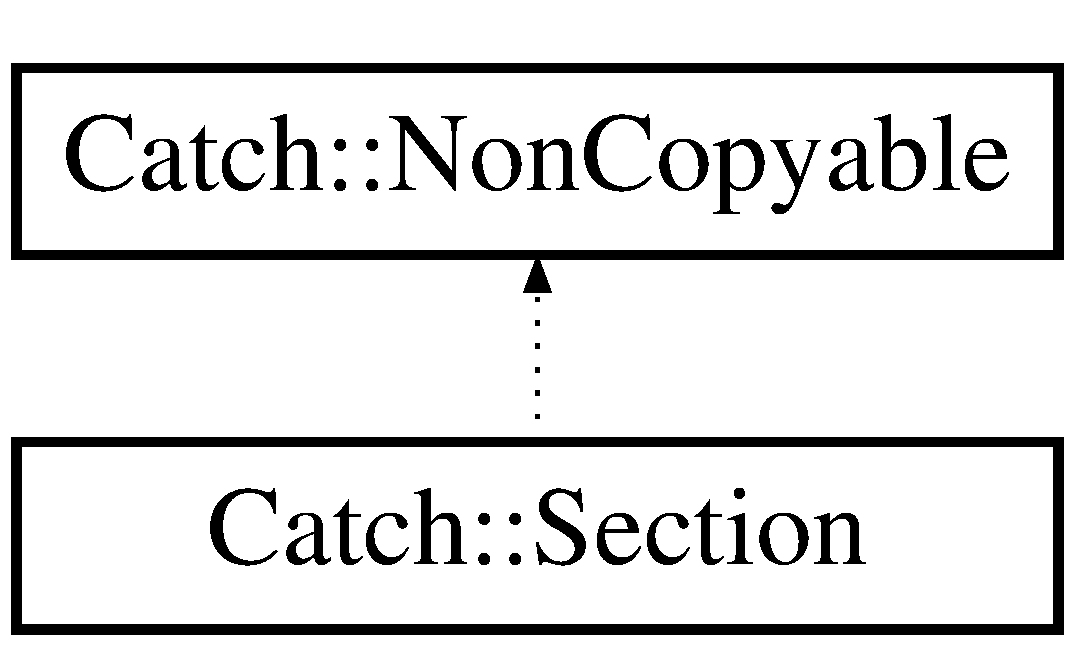
\includegraphics[height=2.000000cm]{class_catch_1_1_section}
\end{center}
\end{figure}
\subsection*{Public Member Functions}
\begin{DoxyCompactItemize}
\item 
\mbox{\Hypertarget{class_catch_1_1_section_a68fd4e51e8981aaa7ddb00d8a6abd099}\label{class_catch_1_1_section_a68fd4e51e8981aaa7ddb00d8a6abd099}} 
{\bfseries Section} (\hyperlink{struct_catch_1_1_section_info}{Section\+Info} const \&info)
\item 
\mbox{\Hypertarget{class_catch_1_1_section_a0632b804dcea1417a2970620a9742eb3}\label{class_catch_1_1_section_a0632b804dcea1417a2970620a9742eb3}} 
{\bfseries operator bool} () const
\end{DoxyCompactItemize}


\subsection{Detailed Description}


Definition at line 2263 of file catch.\+hpp.



The documentation for this class was generated from the following file\+:\begin{DoxyCompactItemize}
\item 
Tests/catch.\+hpp\end{DoxyCompactItemize}

\hypertarget{struct_catch_1_1_section_end_info}{}\section{Catch\+:\+:Section\+End\+Info Struct Reference}
\label{struct_catch_1_1_section_end_info}\index{Catch\+::\+Section\+End\+Info@{Catch\+::\+Section\+End\+Info}}
\subsection*{Public Member Functions}
\begin{DoxyCompactItemize}
\item 
\mbox{\Hypertarget{struct_catch_1_1_section_end_info_abc9381c7c22b6907317ec985ccaa6713}\label{struct_catch_1_1_section_end_info_abc9381c7c22b6907317ec985ccaa6713}} 
{\bfseries Section\+End\+Info} (\hyperlink{struct_catch_1_1_section_info}{Section\+Info} const \&\+\_\+section\+Info, \hyperlink{struct_catch_1_1_counts}{Counts} const \&\+\_\+prev\+Assertions, double \+\_\+duration\+In\+Seconds)
\end{DoxyCompactItemize}
\subsection*{Public Attributes}
\begin{DoxyCompactItemize}
\item 
\mbox{\Hypertarget{struct_catch_1_1_section_end_info_a2d44793392cb83735d086d726822abe9}\label{struct_catch_1_1_section_end_info_a2d44793392cb83735d086d726822abe9}} 
\hyperlink{struct_catch_1_1_section_info}{Section\+Info} {\bfseries section\+Info}
\item 
\mbox{\Hypertarget{struct_catch_1_1_section_end_info_ae70b154cbc05b5dd2901d97f89303d8c}\label{struct_catch_1_1_section_end_info_ae70b154cbc05b5dd2901d97f89303d8c}} 
\hyperlink{struct_catch_1_1_counts}{Counts} {\bfseries prev\+Assertions}
\item 
\mbox{\Hypertarget{struct_catch_1_1_section_end_info_a7c262f2dab9cff166b8eca620c47eea5}\label{struct_catch_1_1_section_end_info_a7c262f2dab9cff166b8eca620c47eea5}} 
double {\bfseries duration\+In\+Seconds}
\end{DoxyCompactItemize}


\subsection{Detailed Description}


Definition at line 2222 of file catch.\+hpp.



The documentation for this struct was generated from the following file\+:\begin{DoxyCompactItemize}
\item 
Tests/catch.\+hpp\end{DoxyCompactItemize}

\hypertarget{struct_catch_1_1_section_info}{}\section{Catch\+:\+:Section\+Info Struct Reference}
\label{struct_catch_1_1_section_info}\index{Catch\+::\+Section\+Info@{Catch\+::\+Section\+Info}}
\subsection*{Public Member Functions}
\begin{DoxyCompactItemize}
\item 
\mbox{\Hypertarget{struct_catch_1_1_section_info_a27aff3aaf8b6611f3651b17111a272c6}\label{struct_catch_1_1_section_info_a27aff3aaf8b6611f3651b17111a272c6}} 
{\bfseries Section\+Info} (\hyperlink{struct_catch_1_1_source_line_info}{Source\+Line\+Info} const \&\+\_\+line\+Info, \textbf{ std\+::string} const \&\+\_\+name, \textbf{ std\+::string} const \&\+\_\+description=\textbf{ std\+::string}())
\end{DoxyCompactItemize}
\subsection*{Public Attributes}
\begin{DoxyCompactItemize}
\item 
\mbox{\Hypertarget{struct_catch_1_1_section_info_a704c8fc662d309137e0d4f199cb7df58}\label{struct_catch_1_1_section_info_a704c8fc662d309137e0d4f199cb7df58}} 
\textbf{ std\+::string} {\bfseries name}
\item 
\mbox{\Hypertarget{struct_catch_1_1_section_info_a0052060219a6de74bb7ade34d4163a4e}\label{struct_catch_1_1_section_info_a0052060219a6de74bb7ade34d4163a4e}} 
\textbf{ std\+::string} {\bfseries description}
\item 
\mbox{\Hypertarget{struct_catch_1_1_section_info_adbc83b8a3507c4acc8ee249e93465711}\label{struct_catch_1_1_section_info_adbc83b8a3507c4acc8ee249e93465711}} 
\hyperlink{struct_catch_1_1_source_line_info}{Source\+Line\+Info} {\bfseries line\+Info}
\end{DoxyCompactItemize}


\subsection{Detailed Description}


Definition at line 2211 of file catch.\+hpp.



The documentation for this struct was generated from the following file\+:\begin{DoxyCompactItemize}
\item 
Tests/catch.\+hpp\end{DoxyCompactItemize}

\hypertarget{struct_catch_1_1_shared_impl}{}\section{Catch\+:\+:Shared\+Impl$<$ T $>$ Struct Template Reference}
\label{struct_catch_1_1_shared_impl}\index{Catch\+::\+Shared\+Impl$<$ T $>$@{Catch\+::\+Shared\+Impl$<$ T $>$}}
Inheritance diagram for Catch\+:\+:Shared\+Impl$<$ T $>$\+:\begin{figure}[H]
\begin{center}
\leavevmode
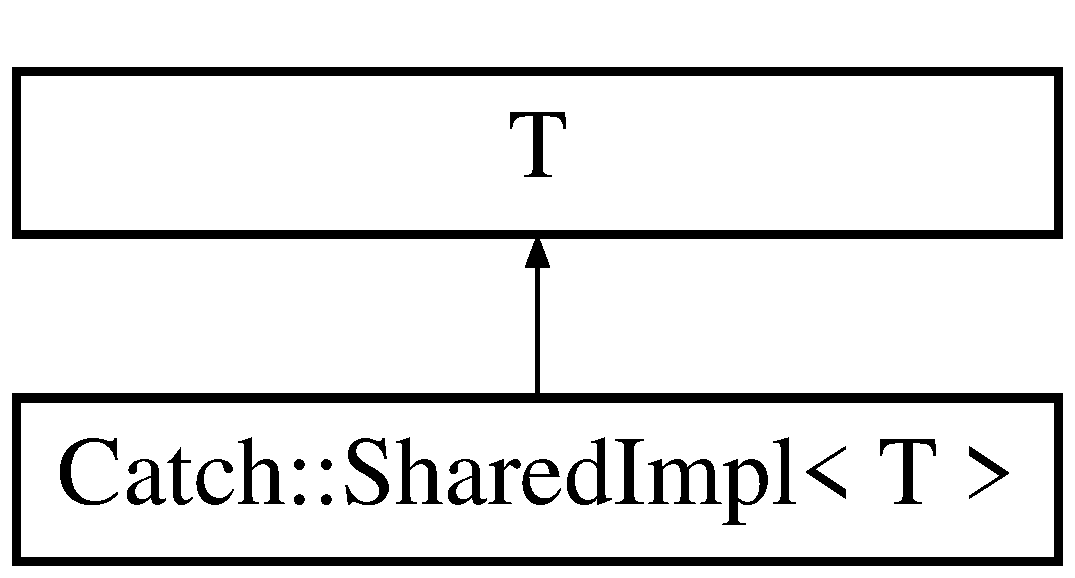
\includegraphics[height=2.000000cm]{struct_catch_1_1_shared_impl}
\end{center}
\end{figure}
\subsection*{Public Member Functions}
\begin{DoxyCompactItemize}
\item 
\mbox{\Hypertarget{struct_catch_1_1_shared_impl_a5d1a4c96e8fc07c821890fd09749062e}\label{struct_catch_1_1_shared_impl_a5d1a4c96e8fc07c821890fd09749062e}} 
virtual void {\bfseries add\+Ref} () const
\item 
\mbox{\Hypertarget{struct_catch_1_1_shared_impl_ada8052c6f24fd73ec099333626f106fe}\label{struct_catch_1_1_shared_impl_ada8052c6f24fd73ec099333626f106fe}} 
virtual void {\bfseries release} () const
\end{DoxyCompactItemize}
\subsection*{Public Attributes}
\begin{DoxyCompactItemize}
\item 
\mbox{\Hypertarget{struct_catch_1_1_shared_impl_a7e71ef1985b85aa41a1632f932a96bcb}\label{struct_catch_1_1_shared_impl_a7e71ef1985b85aa41a1632f932a96bcb}} 
unsigned int {\bfseries m\+\_\+rc}
\end{DoxyCompactItemize}


\subsection{Detailed Description}
\subsubsection*{template$<$typename T = I\+Shared$>$\newline
struct Catch\+::\+Shared\+Impl$<$ T $>$}



Definition at line 509 of file catch.\+hpp.



The documentation for this struct was generated from the following file\+:\begin{DoxyCompactItemize}
\item 
Tests/catch.\+hpp\end{DoxyCompactItemize}

\hypertarget{struct_catch_1_1_source_line_info}{}\section{Catch\+:\+:Source\+Line\+Info Struct Reference}
\label{struct_catch_1_1_source_line_info}\index{Catch\+::\+Source\+Line\+Info@{Catch\+::\+Source\+Line\+Info}}
\subsection*{Public Member Functions}
\begin{DoxyCompactItemize}
\item 
\mbox{\Hypertarget{struct_catch_1_1_source_line_info_a6218cb890337d37f708ea94063958940}\label{struct_catch_1_1_source_line_info_a6218cb890337d37f708ea94063958940}} 
{\bfseries Source\+Line\+Info} (char const $\ast$\+\_\+file, \textbf{ std\+::size\+\_\+t} \+\_\+line)
\item 
\mbox{\Hypertarget{struct_catch_1_1_source_line_info_a1ec99cc0547ce5909133aaa8f14ed4b1}\label{struct_catch_1_1_source_line_info_a1ec99cc0547ce5909133aaa8f14ed4b1}} 
{\bfseries Source\+Line\+Info} (\hyperlink{struct_catch_1_1_source_line_info}{Source\+Line\+Info} const \&other)
\item 
\mbox{\Hypertarget{struct_catch_1_1_source_line_info_a05ab6444e9de7e9c3e76d8aa00093c3a}\label{struct_catch_1_1_source_line_info_a05ab6444e9de7e9c3e76d8aa00093c3a}} 
bool {\bfseries empty} () const
\item 
\mbox{\Hypertarget{struct_catch_1_1_source_line_info_a688e761986879266658f000f14ab8a42}\label{struct_catch_1_1_source_line_info_a688e761986879266658f000f14ab8a42}} 
bool {\bfseries operator==} (\hyperlink{struct_catch_1_1_source_line_info}{Source\+Line\+Info} const \&other) const
\item 
\mbox{\Hypertarget{struct_catch_1_1_source_line_info_a8b99a0d7b1553d8c2298c694db924be3}\label{struct_catch_1_1_source_line_info_a8b99a0d7b1553d8c2298c694db924be3}} 
bool {\bfseries operator$<$} (\hyperlink{struct_catch_1_1_source_line_info}{Source\+Line\+Info} const \&other) const
\end{DoxyCompactItemize}
\subsection*{Public Attributes}
\begin{DoxyCompactItemize}
\item 
\mbox{\Hypertarget{struct_catch_1_1_source_line_info_adf3ccf0c2bd326eb3466318af82a94dd}\label{struct_catch_1_1_source_line_info_adf3ccf0c2bd326eb3466318af82a94dd}} 
\textbf{ std\+::string} {\bfseries file}
\item 
\mbox{\Hypertarget{struct_catch_1_1_source_line_info_a841e5d696c7b9cde24e45e61dd979c77}\label{struct_catch_1_1_source_line_info_a841e5d696c7b9cde24e45e61dd979c77}} 
\textbf{ std\+::size\+\_\+t} {\bfseries line}
\end{DoxyCompactItemize}


\subsection{Detailed Description}


Definition at line 348 of file catch.\+hpp.



The documentation for this struct was generated from the following file\+:\begin{DoxyCompactItemize}
\item 
Tests/catch.\+hpp\end{DoxyCompactItemize}

\hypertarget{class_square}{}\section{Square Class Reference}
\label{class_square}\index{Square@{Square}}


The \hyperlink{class_square}{Square} class It represents a graphical case. It is actually a Q\+Label that contains a image.  




{\ttfamily \#include $<$square.\+h$>$}

Inheritance diagram for Square\+:\begin{figure}[H]
\begin{center}
\leavevmode
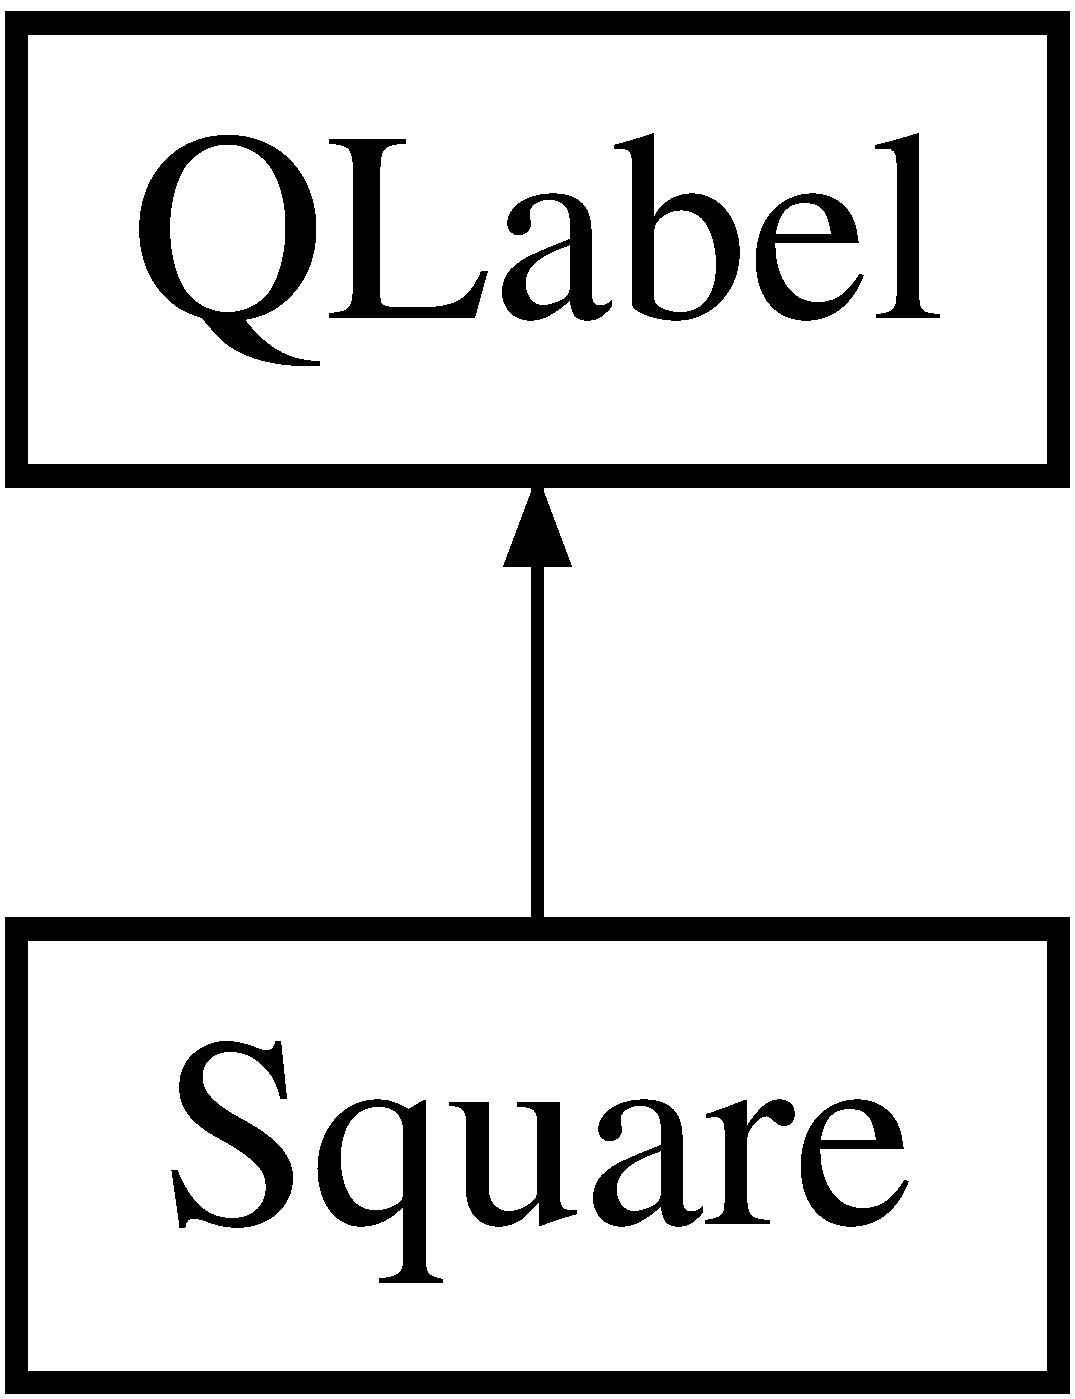
\includegraphics[height=2.000000cm]{class_square}
\end{center}
\end{figure}
\subsection*{Public Member Functions}
\begin{DoxyCompactItemize}
\item 
\hyperlink{class_square_a6fa43122d0022ee5553962b05bd8ecd4}{Square} (int column, int row)
\begin{DoxyCompactList}\small\item\em \hyperlink{class_square}{Square}, the constructor Creates an instance of the class. \end{DoxyCompactList}\item 
\mbox{\Hypertarget{class_square_ab6c220a623d0d0f4793828063728dc10}\label{class_square_ab6c220a623d0d0f4793828063728dc10}} 
\hyperlink{class_square_ab6c220a623d0d0f4793828063728dc10}{$\sim$\+Square} ()=default
\begin{DoxyCompactList}\small\item\em $\sim$\+Square, the destructor. Destroy all the elements of the class that need to be. \end{DoxyCompactList}\item 
void \hyperlink{class_square_a7a7e3e8e985f790b9a28cb4f5a6dab7a}{set\+Img} (\textbf{ string} path)
\begin{DoxyCompactList}\small\item\em set\+Img Sets an image as Pixmap of the Q\+Label \end{DoxyCompactList}\item 
int \hyperlink{class_square_ad3391313a44cdbfbe87fd3ddc545feac}{get\+Row} ()
\begin{DoxyCompactList}\small\item\em get\+Row Returns the row of the Q\+Grid\+Layout the \hyperlink{class_square}{Square} is in. \end{DoxyCompactList}\item 
int \hyperlink{class_square_aaf011d4ff750d0770ba82b4c659c27f8}{get\+Col} ()
\begin{DoxyCompactList}\small\item\em get\+Col Returns the column of the Q\+Grid\+Layout the \hyperlink{class_square}{Square} is in. \end{DoxyCompactList}\end{DoxyCompactItemize}


\subsection{Detailed Description}
The \hyperlink{class_square}{Square} class It represents a graphical case. It is actually a Q\+Label that contains a image. 

Definition at line 15 of file square.\+h.



\subsection{Constructor \& Destructor Documentation}
\mbox{\Hypertarget{class_square_a6fa43122d0022ee5553962b05bd8ecd4}\label{class_square_a6fa43122d0022ee5553962b05bd8ecd4}} 
\index{Square@{Square}!Square@{Square}}
\index{Square@{Square}!Square@{Square}}
\subsubsection{\texorpdfstring{Square()}{Square()}}
{\footnotesize\ttfamily Square\+::\+Square (\begin{DoxyParamCaption}\item[{int}]{column,  }\item[{int}]{row }\end{DoxyParamCaption})}



\hyperlink{class_square}{Square}, the constructor Creates an instance of the class. 


\begin{DoxyParams}{Parameters}
{\em column} & the column of the Q\+Grid\+Layout it is contained in. \\
\hline
{\em row} & the row of the Q\+Grid\+Layout it is contained in. \\
\hline
\end{DoxyParams}


Definition at line 8 of file square.\+cpp.



\subsection{Member Function Documentation}
\mbox{\Hypertarget{class_square_aaf011d4ff750d0770ba82b4c659c27f8}\label{class_square_aaf011d4ff750d0770ba82b4c659c27f8}} 
\index{Square@{Square}!get\+Col@{get\+Col}}
\index{get\+Col@{get\+Col}!Square@{Square}}
\subsubsection{\texorpdfstring{get\+Col()}{getCol()}}
{\footnotesize\ttfamily int Square\+::get\+Col (\begin{DoxyParamCaption}{ }\end{DoxyParamCaption})\hspace{0.3cm}{\ttfamily [inline]}}



get\+Col Returns the column of the Q\+Grid\+Layout the \hyperlink{class_square}{Square} is in. 

\begin{DoxyReturn}{Returns}
an int, the column. 
\end{DoxyReturn}


Definition at line 56 of file square.\+h.

\mbox{\Hypertarget{class_square_ad3391313a44cdbfbe87fd3ddc545feac}\label{class_square_ad3391313a44cdbfbe87fd3ddc545feac}} 
\index{Square@{Square}!get\+Row@{get\+Row}}
\index{get\+Row@{get\+Row}!Square@{Square}}
\subsubsection{\texorpdfstring{get\+Row()}{getRow()}}
{\footnotesize\ttfamily int Square\+::get\+Row (\begin{DoxyParamCaption}{ }\end{DoxyParamCaption})\hspace{0.3cm}{\ttfamily [inline]}}



get\+Row Returns the row of the Q\+Grid\+Layout the \hyperlink{class_square}{Square} is in. 

\begin{DoxyReturn}{Returns}
an int, the row. 
\end{DoxyReturn}


Definition at line 60 of file square.\+h.

\mbox{\Hypertarget{class_square_a7a7e3e8e985f790b9a28cb4f5a6dab7a}\label{class_square_a7a7e3e8e985f790b9a28cb4f5a6dab7a}} 
\index{Square@{Square}!set\+Img@{set\+Img}}
\index{set\+Img@{set\+Img}!Square@{Square}}
\subsubsection{\texorpdfstring{set\+Img()}{setImg()}}
{\footnotesize\ttfamily void Square\+::set\+Img (\begin{DoxyParamCaption}\item[{\textbf{ string}}]{path }\end{DoxyParamCaption})}



set\+Img Sets an image as Pixmap of the Q\+Label 


\begin{DoxyParams}{Parameters}
{\em path} & the relative path to the image. \\
\hline
\end{DoxyParams}


Definition at line 13 of file square.\+cpp.



The documentation for this class was generated from the following files\+:\begin{DoxyCompactItemize}
\item 
Application/square.\+h\item 
Application/square.\+cpp\end{DoxyCompactItemize}

\hypertarget{class_ui_1_1start_screen}{}\section{Ui\+:\+:start\+Screen Class Reference}
\label{class_ui_1_1start_screen}\index{Ui\+::start\+Screen@{Ui\+::start\+Screen}}
Inheritance diagram for Ui\+:\+:start\+Screen\+:\begin{figure}[H]
\begin{center}
\leavevmode
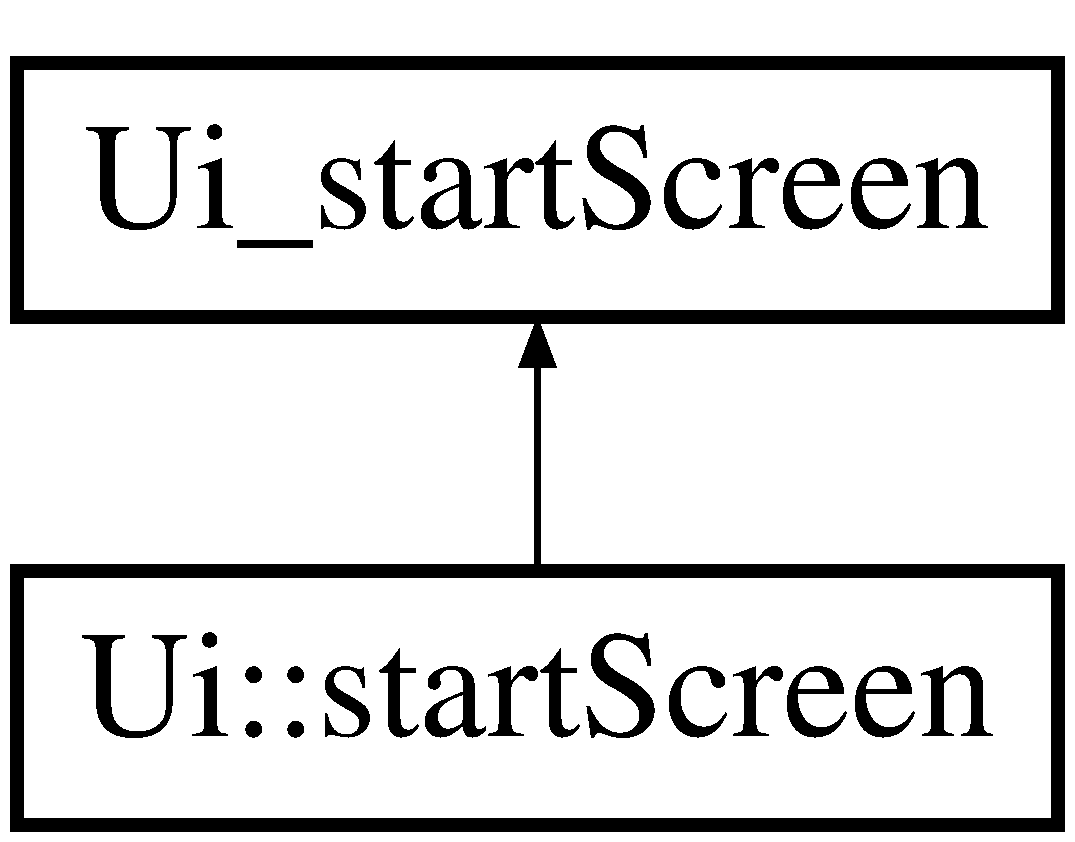
\includegraphics[height=2.000000cm]{class_ui_1_1start_screen}
\end{center}
\end{figure}
\subsection*{Additional Inherited Members}


\subsection{Detailed Description}


Definition at line 287 of file ui\+\_\+startscreen.\+h.



The documentation for this class was generated from the following file\+:\begin{DoxyCompactItemize}
\item 
Application/ui\+\_\+startscreen.\+h\end{DoxyCompactItemize}

\hypertarget{struct_catch_1_1_matchers_1_1_impl_1_1_std_string_1_1_starts_with}{}\section{Catch\+:\+:Matchers\+:\+:Impl\+:\+:Std\+String\+:\+:Starts\+With Struct Reference}
\label{struct_catch_1_1_matchers_1_1_impl_1_1_std_string_1_1_starts_with}\index{Catch\+::\+Matchers\+::\+Impl\+::\+Std\+String\+::\+Starts\+With@{Catch\+::\+Matchers\+::\+Impl\+::\+Std\+String\+::\+Starts\+With}}
Inheritance diagram for Catch\+:\+:Matchers\+:\+:Impl\+:\+:Std\+String\+:\+:Starts\+With\+:\begin{figure}[H]
\begin{center}
\leavevmode
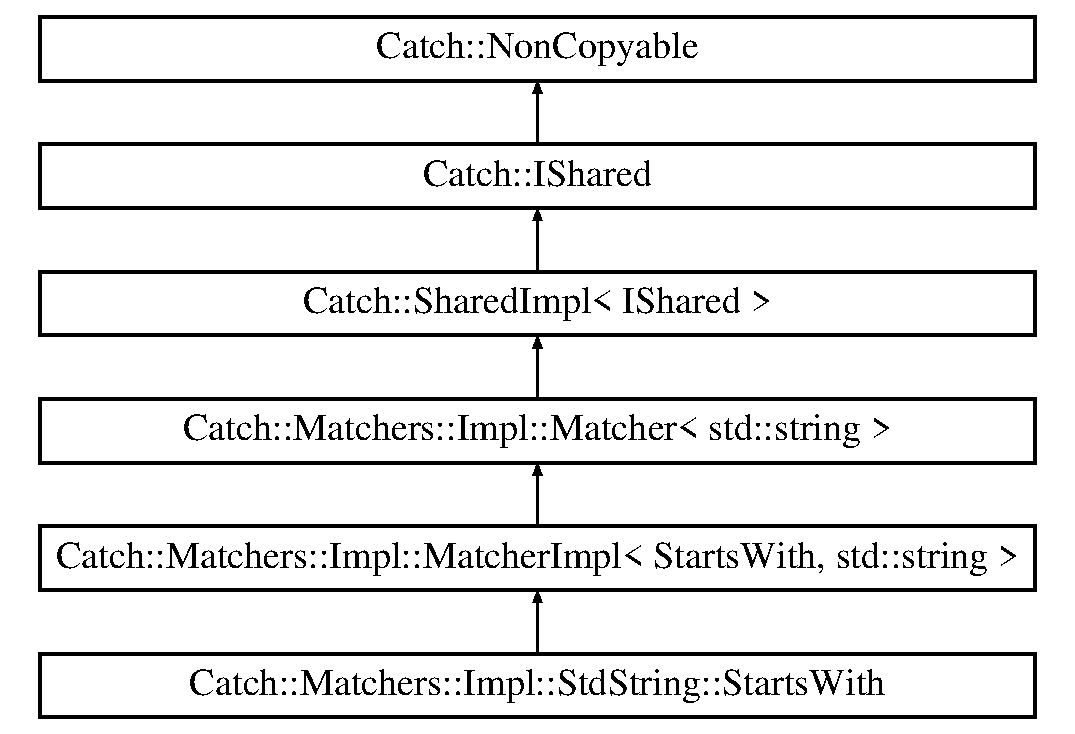
\includegraphics[height=6.000000cm]{struct_catch_1_1_matchers_1_1_impl_1_1_std_string_1_1_starts_with}
\end{center}
\end{figure}
\subsection*{Public Member Functions}
\begin{DoxyCompactItemize}
\item 
\mbox{\Hypertarget{struct_catch_1_1_matchers_1_1_impl_1_1_std_string_1_1_starts_with_a0db1bd8876219464ae60346c9525bcf6}\label{struct_catch_1_1_matchers_1_1_impl_1_1_std_string_1_1_starts_with_a0db1bd8876219464ae60346c9525bcf6}} 
{\bfseries Starts\+With} (\textbf{ std\+::string} const \&substr, Case\+Sensitive\+::\+Choice case\+Sensitivity=Case\+Sensitive\+::\+Yes)
\item 
\mbox{\Hypertarget{struct_catch_1_1_matchers_1_1_impl_1_1_std_string_1_1_starts_with_a5526cb587632e7e46253d6f60ae01098}\label{struct_catch_1_1_matchers_1_1_impl_1_1_std_string_1_1_starts_with_a5526cb587632e7e46253d6f60ae01098}} 
{\bfseries Starts\+With} (\hyperlink{struct_catch_1_1_matchers_1_1_impl_1_1_std_string_1_1_starts_with}{Starts\+With} const \&other)
\item 
\mbox{\Hypertarget{struct_catch_1_1_matchers_1_1_impl_1_1_std_string_1_1_starts_with_ab8f8d15e06d7ec13fee7d9ec4075dafa}\label{struct_catch_1_1_matchers_1_1_impl_1_1_std_string_1_1_starts_with_ab8f8d15e06d7ec13fee7d9ec4075dafa}} 
virtual bool {\bfseries match} (\textbf{ std\+::string} const \&expr) const
\item 
\mbox{\Hypertarget{struct_catch_1_1_matchers_1_1_impl_1_1_std_string_1_1_starts_with_a85a24e2ac23025edbe31cbf5bb755fb3}\label{struct_catch_1_1_matchers_1_1_impl_1_1_std_string_1_1_starts_with_a85a24e2ac23025edbe31cbf5bb755fb3}} 
virtual \textbf{ std\+::string} {\bfseries to\+String} () const
\end{DoxyCompactItemize}
\subsection*{Public Attributes}
\begin{DoxyCompactItemize}
\item 
\mbox{\Hypertarget{struct_catch_1_1_matchers_1_1_impl_1_1_std_string_1_1_starts_with_accaace83106244c635d251addb028125}\label{struct_catch_1_1_matchers_1_1_impl_1_1_std_string_1_1_starts_with_accaace83106244c635d251addb028125}} 
\hyperlink{struct_catch_1_1_matchers_1_1_impl_1_1_std_string_1_1_cased_string}{Cased\+String} {\bfseries m\+\_\+data}
\end{DoxyCompactItemize}
\subsection*{Additional Inherited Members}


\subsection{Detailed Description}


Definition at line 1063 of file catch.\+hpp.



The documentation for this struct was generated from the following file\+:\begin{DoxyCompactItemize}
\item 
Tests/catch.\+hpp\end{DoxyCompactItemize}

\hypertarget{struct_catch_1_1_stream_end_stop}{}\section{Catch\+:\+:Stream\+End\+Stop Struct Reference}
\label{struct_catch_1_1_stream_end_stop}\index{Catch\+::\+Stream\+End\+Stop@{Catch\+::\+Stream\+End\+Stop}}
\subsection*{Public Member Functions}
\begin{DoxyCompactItemize}
\item 
\mbox{\Hypertarget{struct_catch_1_1_stream_end_stop_a3025092e06c224e0845f2caa07b26d0e}\label{struct_catch_1_1_stream_end_stop_a3025092e06c224e0845f2caa07b26d0e}} 
\textbf{ std\+::string} {\bfseries operator+} ()
\end{DoxyCompactItemize}


\subsection{Detailed Description}


Definition at line 382 of file catch.\+hpp.



The documentation for this struct was generated from the following file\+:\begin{DoxyCompactItemize}
\item 
Tests/catch.\+hpp\end{DoxyCompactItemize}

\hypertarget{struct_catch_1_1_string_maker}{}\section{Catch\+:\+:String\+Maker$<$ T $>$ Struct Template Reference}
\label{struct_catch_1_1_string_maker}\index{Catch\+::\+String\+Maker$<$ T $>$@{Catch\+::\+String\+Maker$<$ T $>$}}
Inheritance diagram for Catch\+:\+:String\+Maker$<$ T $>$\+:\begin{figure}[H]
\begin{center}
\leavevmode
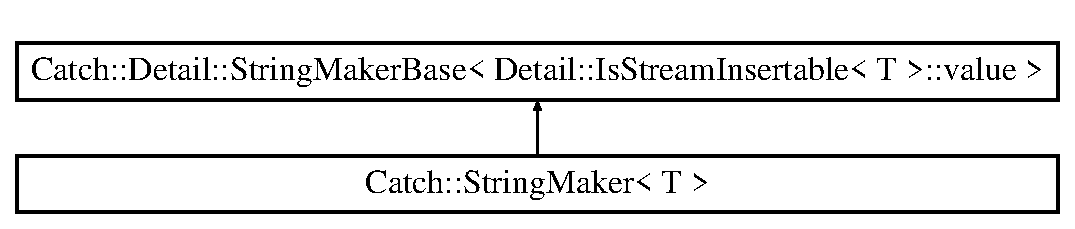
\includegraphics[height=2.000000cm]{struct_catch_1_1_string_maker}
\end{center}
\end{figure}
\subsection*{Additional Inherited Members}


\subsection{Detailed Description}
\subsubsection*{template$<$typename T$>$\newline
struct Catch\+::\+String\+Maker$<$ T $>$}



Definition at line 1632 of file catch.\+hpp.



The documentation for this struct was generated from the following file\+:\begin{DoxyCompactItemize}
\item 
Tests/catch.\+hpp\end{DoxyCompactItemize}

\hypertarget{struct_catch_1_1_string_maker_3_01_r_01_c_1_1_5_01_4}{}\section{Catch\+:\+:String\+Maker$<$ R C\+:\+:$\ast$ $>$ Struct Template Reference}
\label{struct_catch_1_1_string_maker_3_01_r_01_c_1_1_5_01_4}\index{Catch\+::\+String\+Maker$<$ R C\+::$\ast$ $>$@{Catch\+::\+String\+Maker$<$ R C\+::$\ast$ $>$}}
\subsection*{Static Public Member Functions}
\begin{DoxyCompactItemize}
\item 
\mbox{\Hypertarget{struct_catch_1_1_string_maker_3_01_r_01_c_1_1_5_01_4_af69c15e0b406e945777137fe4a333731}\label{struct_catch_1_1_string_maker_3_01_r_01_c_1_1_5_01_4_af69c15e0b406e945777137fe4a333731}} 
static \textbf{ std\+::string} {\bfseries convert} (R C\+::$\ast$p)
\end{DoxyCompactItemize}


\subsection{Detailed Description}
\subsubsection*{template$<$typename R, typename C$>$\newline
struct Catch\+::\+String\+Maker$<$ R C\+::$\ast$ $>$}



Definition at line 1647 of file catch.\+hpp.



The documentation for this struct was generated from the following file\+:\begin{DoxyCompactItemize}
\item 
Tests/catch.\+hpp\end{DoxyCompactItemize}

\hypertarget{struct_catch_1_1_string_maker_3_01_t_01_5_01_4}{}\section{Catch\+:\+:String\+Maker$<$ T $\ast$ $>$ Struct Template Reference}
\label{struct_catch_1_1_string_maker_3_01_t_01_5_01_4}\index{Catch\+::\+String\+Maker$<$ T $\ast$ $>$@{Catch\+::\+String\+Maker$<$ T $\ast$ $>$}}
\subsection*{Static Public Member Functions}
\begin{DoxyCompactItemize}
\item 
\mbox{\Hypertarget{struct_catch_1_1_string_maker_3_01_t_01_5_01_4_a2adbc75c99d71b8323f4052bcb0815c9}\label{struct_catch_1_1_string_maker_3_01_t_01_5_01_4_a2adbc75c99d71b8323f4052bcb0815c9}} 
{\footnotesize template$<$typename U $>$ }\\static \textbf{ std\+::string} {\bfseries convert} (U $\ast$p)
\end{DoxyCompactItemize}


\subsection{Detailed Description}
\subsubsection*{template$<$typename T$>$\newline
struct Catch\+::\+String\+Maker$<$ T $\ast$ $>$}



Definition at line 1636 of file catch.\+hpp.



The documentation for this struct was generated from the following file\+:\begin{DoxyCompactItemize}
\item 
Tests/catch.\+hpp\end{DoxyCompactItemize}

\hypertarget{struct_catch_1_1_detail_1_1_string_maker_base}{}\section{Catch\+:\+:Detail\+:\+:String\+Maker\+Base$<$ C $>$ Struct Template Reference}
\label{struct_catch_1_1_detail_1_1_string_maker_base}\index{Catch\+::\+Detail\+::\+String\+Maker\+Base$<$ C $>$@{Catch\+::\+Detail\+::\+String\+Maker\+Base$<$ C $>$}}
\subsection*{Static Public Member Functions}
\begin{DoxyCompactItemize}
\item 
\mbox{\Hypertarget{struct_catch_1_1_detail_1_1_string_maker_base_a8eb9f635dc413a5758e22614bafaf1a3}\label{struct_catch_1_1_detail_1_1_string_maker_base_a8eb9f635dc413a5758e22614bafaf1a3}} 
{\footnotesize template$<$typename T $>$ }\\static \textbf{ std\+::string} {\bfseries convert} (T const \&)
\end{DoxyCompactItemize}


\subsection{Detailed Description}
\subsubsection*{template$<$bool C$>$\newline
struct Catch\+::\+Detail\+::\+String\+Maker\+Base$<$ C $>$}



Definition at line 1599 of file catch.\+hpp.



The documentation for this struct was generated from the following file\+:\begin{DoxyCompactItemize}
\item 
Tests/catch.\+hpp\end{DoxyCompactItemize}

\hypertarget{struct_catch_1_1_detail_1_1_string_maker_base_3_01true_01_4}{}\section{Catch\+:\+:Detail\+:\+:String\+Maker\+Base$<$ true $>$ Struct Template Reference}
\label{struct_catch_1_1_detail_1_1_string_maker_base_3_01true_01_4}\index{Catch\+::\+Detail\+::\+String\+Maker\+Base$<$ true $>$@{Catch\+::\+Detail\+::\+String\+Maker\+Base$<$ true $>$}}
\subsection*{Static Public Member Functions}
\begin{DoxyCompactItemize}
\item 
\mbox{\Hypertarget{struct_catch_1_1_detail_1_1_string_maker_base_3_01true_01_4_af9b5fdf7fddd8c5c873caa819e5f00f6}\label{struct_catch_1_1_detail_1_1_string_maker_base_3_01true_01_4_af9b5fdf7fddd8c5c873caa819e5f00f6}} 
{\footnotesize template$<$typename T $>$ }\\static \textbf{ std\+::string} {\bfseries convert} (T const \&\+\_\+value)
\end{DoxyCompactItemize}


\subsection{Detailed Description}
\subsubsection*{template$<$$>$\newline
struct Catch\+::\+Detail\+::\+String\+Maker\+Base$<$ true $>$}



Definition at line 1613 of file catch.\+hpp.



The documentation for this struct was generated from the following file\+:\begin{DoxyCompactItemize}
\item 
Tests/catch.\+hpp\end{DoxyCompactItemize}

\hypertarget{struct_catch_1_1_tag_alias}{}\section{Catch\+:\+:Tag\+Alias Struct Reference}
\label{struct_catch_1_1_tag_alias}\index{Catch\+::\+Tag\+Alias@{Catch\+::\+Tag\+Alias}}
\subsection*{Public Member Functions}
\begin{DoxyCompactItemize}
\item 
\mbox{\Hypertarget{struct_catch_1_1_tag_alias_ad9124d03bfb6f767f1c97572330b05bc}\label{struct_catch_1_1_tag_alias_ad9124d03bfb6f767f1c97572330b05bc}} 
{\bfseries Tag\+Alias} (\textbf{ std\+::string} \+\_\+tag, \hyperlink{struct_catch_1_1_source_line_info}{Source\+Line\+Info} \+\_\+line\+Info)
\end{DoxyCompactItemize}
\subsection*{Public Attributes}
\begin{DoxyCompactItemize}
\item 
\mbox{\Hypertarget{struct_catch_1_1_tag_alias_a950183883ab17c90d0fab16b966b6e2d}\label{struct_catch_1_1_tag_alias_a950183883ab17c90d0fab16b966b6e2d}} 
\textbf{ std\+::string} {\bfseries tag}
\item 
\mbox{\Hypertarget{struct_catch_1_1_tag_alias_a2f51fe0b3c052561275d26b6eb88f702}\label{struct_catch_1_1_tag_alias_a2f51fe0b3c052561275d26b6eb88f702}} 
\hyperlink{struct_catch_1_1_source_line_info}{Source\+Line\+Info} {\bfseries line\+Info}
\end{DoxyCompactItemize}


\subsection{Detailed Description}


Definition at line 2662 of file catch.\+hpp.



The documentation for this struct was generated from the following file\+:\begin{DoxyCompactItemize}
\item 
Tests/catch.\+hpp\end{DoxyCompactItemize}

\hypertarget{class_catch_1_1_test_case}{}\section{Catch\+:\+:Test\+Case Class Reference}
\label{class_catch_1_1_test_case}\index{Catch\+::\+Test\+Case@{Catch\+::\+Test\+Case}}
Inheritance diagram for Catch\+:\+:Test\+Case\+:\begin{figure}[H]
\begin{center}
\leavevmode
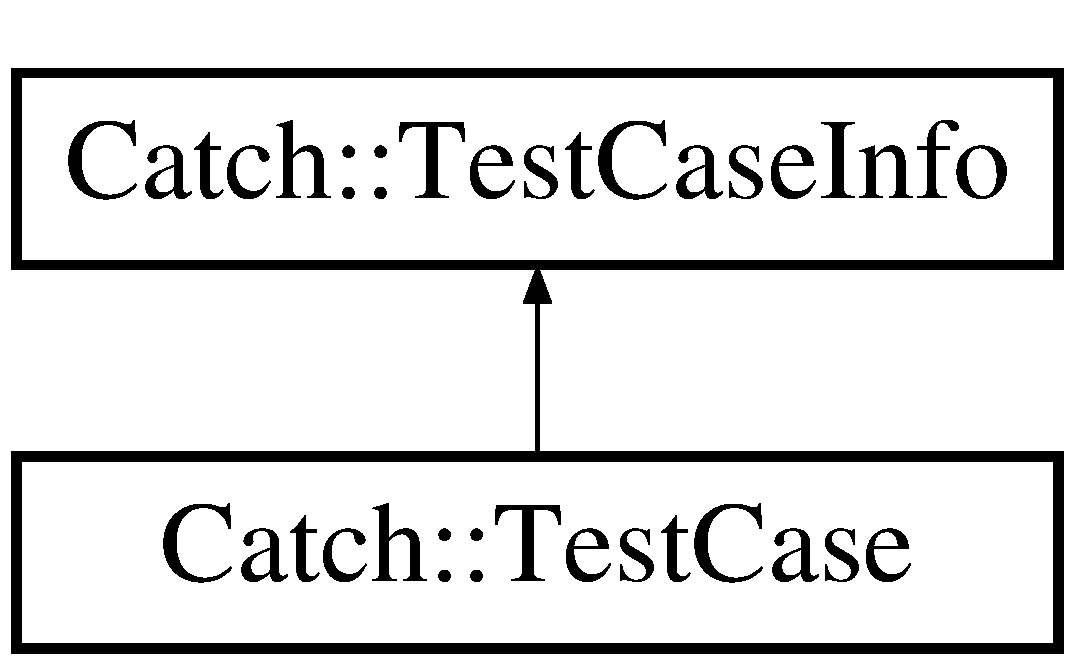
\includegraphics[height=2.000000cm]{class_catch_1_1_test_case}
\end{center}
\end{figure}
\subsection*{Public Member Functions}
\begin{DoxyCompactItemize}
\item 
\mbox{\Hypertarget{class_catch_1_1_test_case_a03a5b913484681bd6d398dc5e9c2a907}\label{class_catch_1_1_test_case_a03a5b913484681bd6d398dc5e9c2a907}} 
{\bfseries Test\+Case} (\hyperlink{struct_catch_1_1_i_test_case}{I\+Test\+Case} $\ast$test\+Case, \hyperlink{struct_catch_1_1_test_case_info}{Test\+Case\+Info} const \&info)
\item 
\mbox{\Hypertarget{class_catch_1_1_test_case_ac0011d3789edc3e44edb41f13c4775a0}\label{class_catch_1_1_test_case_ac0011d3789edc3e44edb41f13c4775a0}} 
{\bfseries Test\+Case} (\hyperlink{class_catch_1_1_test_case}{Test\+Case} const \&other)
\item 
\mbox{\Hypertarget{class_catch_1_1_test_case_a0812e8a216d09b087d5874687009f0d6}\label{class_catch_1_1_test_case_a0812e8a216d09b087d5874687009f0d6}} 
\hyperlink{class_catch_1_1_test_case}{Test\+Case} {\bfseries with\+Name} (\textbf{ std\+::string} const \&\+\_\+new\+Name) const
\item 
\mbox{\Hypertarget{class_catch_1_1_test_case_a26f346c8446dded0562fe3818ae71651}\label{class_catch_1_1_test_case_a26f346c8446dded0562fe3818ae71651}} 
void {\bfseries invoke} () const
\item 
\mbox{\Hypertarget{class_catch_1_1_test_case_a1ea0d79f49156cebea076fe1ba50d2b6}\label{class_catch_1_1_test_case_a1ea0d79f49156cebea076fe1ba50d2b6}} 
\hyperlink{struct_catch_1_1_test_case_info}{Test\+Case\+Info} const  \& {\bfseries get\+Test\+Case\+Info} () const
\item 
\mbox{\Hypertarget{class_catch_1_1_test_case_aee38f908faf10b905b209ca388275413}\label{class_catch_1_1_test_case_aee38f908faf10b905b209ca388275413}} 
void {\bfseries swap} (\hyperlink{class_catch_1_1_test_case}{Test\+Case} \&other)
\item 
\mbox{\Hypertarget{class_catch_1_1_test_case_a5456d03a90f75292835c158f3a3374a1}\label{class_catch_1_1_test_case_a5456d03a90f75292835c158f3a3374a1}} 
bool {\bfseries operator==} (\hyperlink{class_catch_1_1_test_case}{Test\+Case} const \&other) const
\item 
\mbox{\Hypertarget{class_catch_1_1_test_case_a030e4b9282e9b32e08c8bd5e5cd6fa98}\label{class_catch_1_1_test_case_a030e4b9282e9b32e08c8bd5e5cd6fa98}} 
bool {\bfseries operator$<$} (\hyperlink{class_catch_1_1_test_case}{Test\+Case} const \&other) const
\item 
\mbox{\Hypertarget{class_catch_1_1_test_case_a8022e3f74232f7887d2d2cbbc8876502}\label{class_catch_1_1_test_case_a8022e3f74232f7887d2d2cbbc8876502}} 
\hyperlink{class_catch_1_1_test_case}{Test\+Case} \& {\bfseries operator=} (\hyperlink{class_catch_1_1_test_case}{Test\+Case} const \&other)
\end{DoxyCompactItemize}
\subsection*{Additional Inherited Members}


\subsection{Detailed Description}


Definition at line 2804 of file catch.\+hpp.



The documentation for this class was generated from the following file\+:\begin{DoxyCompactItemize}
\item 
Tests/catch.\+hpp\end{DoxyCompactItemize}

\hypertarget{struct_catch_1_1_test_case_info}{}\section{Catch\+:\+:Test\+Case\+Info Struct Reference}
\label{struct_catch_1_1_test_case_info}\index{Catch\+::\+Test\+Case\+Info@{Catch\+::\+Test\+Case\+Info}}
Inheritance diagram for Catch\+:\+:Test\+Case\+Info\+:\begin{figure}[H]
\begin{center}
\leavevmode
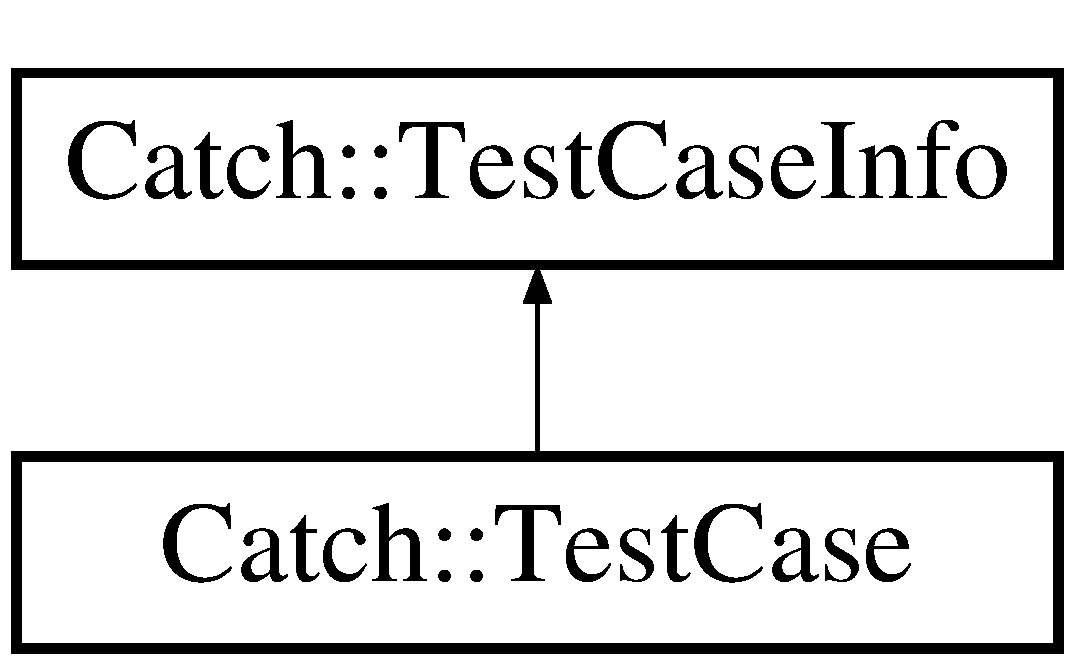
\includegraphics[height=2.000000cm]{struct_catch_1_1_test_case_info}
\end{center}
\end{figure}
\subsection*{Public Types}
\begin{DoxyCompactItemize}
\item 
\mbox{\Hypertarget{struct_catch_1_1_test_case_info_a39b232f74b4a7a6f2183b96759027eac}\label{struct_catch_1_1_test_case_info_a39b232f74b4a7a6f2183b96759027eac}} 
enum {\bfseries Special\+Properties} \{ \newline
{\bfseries None} = 0, 
{\bfseries Is\+Hidden} = 1 $<$$<$ 1, 
{\bfseries Should\+Fail} = 1 $<$$<$ 2, 
{\bfseries May\+Fail} = 1 $<$$<$ 3, 
\newline
{\bfseries Throws} = 1 $<$$<$ 4
 \}
\end{DoxyCompactItemize}
\subsection*{Public Member Functions}
\begin{DoxyCompactItemize}
\item 
\mbox{\Hypertarget{struct_catch_1_1_test_case_info_a35ec65315e0d1f178491b5a59f3f3123}\label{struct_catch_1_1_test_case_info_a35ec65315e0d1f178491b5a59f3f3123}} 
{\bfseries Test\+Case\+Info} (\textbf{ std\+::string} const \&\+\_\+name, \textbf{ std\+::string} const \&\+\_\+class\+Name, \textbf{ std\+::string} const \&\+\_\+description, \textbf{ std\+::set}$<$ \textbf{ std\+::string} $>$ const \&\+\_\+tags, \hyperlink{struct_catch_1_1_source_line_info}{Source\+Line\+Info} const \&\+\_\+line\+Info)
\item 
\mbox{\Hypertarget{struct_catch_1_1_test_case_info_ac338adb4e38f4bf3977fb45b2b1fe447}\label{struct_catch_1_1_test_case_info_ac338adb4e38f4bf3977fb45b2b1fe447}} 
{\bfseries Test\+Case\+Info} (\hyperlink{struct_catch_1_1_test_case_info}{Test\+Case\+Info} const \&other)
\item 
\mbox{\Hypertarget{struct_catch_1_1_test_case_info_a934b1a0952700743e99d62ec1731a2e2}\label{struct_catch_1_1_test_case_info_a934b1a0952700743e99d62ec1731a2e2}} 
bool {\bfseries is\+Hidden} () const
\item 
\mbox{\Hypertarget{struct_catch_1_1_test_case_info_afc70d4379a2070cc22b693ffe3932c1a}\label{struct_catch_1_1_test_case_info_afc70d4379a2070cc22b693ffe3932c1a}} 
bool {\bfseries throws} () const
\item 
\mbox{\Hypertarget{struct_catch_1_1_test_case_info_a5f37291295e3a6de2dd85324c941edaf}\label{struct_catch_1_1_test_case_info_a5f37291295e3a6de2dd85324c941edaf}} 
bool {\bfseries ok\+To\+Fail} () const
\item 
\mbox{\Hypertarget{struct_catch_1_1_test_case_info_abe33d81233230cdae8afa714688e905b}\label{struct_catch_1_1_test_case_info_abe33d81233230cdae8afa714688e905b}} 
bool {\bfseries expected\+To\+Fail} () const
\end{DoxyCompactItemize}
\subsection*{Public Attributes}
\begin{DoxyCompactItemize}
\item 
\mbox{\Hypertarget{struct_catch_1_1_test_case_info_a463794e2f5cfead307c93efd134ade36}\label{struct_catch_1_1_test_case_info_a463794e2f5cfead307c93efd134ade36}} 
\textbf{ std\+::string} {\bfseries name}
\item 
\mbox{\Hypertarget{struct_catch_1_1_test_case_info_a1a5e0825132a38d091defdebbf2f8ce9}\label{struct_catch_1_1_test_case_info_a1a5e0825132a38d091defdebbf2f8ce9}} 
\textbf{ std\+::string} {\bfseries class\+Name}
\item 
\mbox{\Hypertarget{struct_catch_1_1_test_case_info_a37fe2db9425bc45f6a33893eac31198e}\label{struct_catch_1_1_test_case_info_a37fe2db9425bc45f6a33893eac31198e}} 
\textbf{ std\+::string} {\bfseries description}
\item 
\mbox{\Hypertarget{struct_catch_1_1_test_case_info_a045f62e7719a8760a5b456f7fd2dc97c}\label{struct_catch_1_1_test_case_info_a045f62e7719a8760a5b456f7fd2dc97c}} 
\textbf{ std\+::set}$<$ \textbf{ std\+::string} $>$ {\bfseries tags}
\item 
\mbox{\Hypertarget{struct_catch_1_1_test_case_info_a0ed3864a313e8ddc3ae38431be5be9ae}\label{struct_catch_1_1_test_case_info_a0ed3864a313e8ddc3ae38431be5be9ae}} 
\textbf{ std\+::set}$<$ \textbf{ std\+::string} $>$ {\bfseries lcase\+Tags}
\item 
\mbox{\Hypertarget{struct_catch_1_1_test_case_info_ac65c2d36fd36f71e9bf782b2ea245c64}\label{struct_catch_1_1_test_case_info_ac65c2d36fd36f71e9bf782b2ea245c64}} 
\textbf{ std\+::string} {\bfseries tags\+As\+String}
\item 
\mbox{\Hypertarget{struct_catch_1_1_test_case_info_aa9407b7f442655b51a2aad24b3fa2fd3}\label{struct_catch_1_1_test_case_info_aa9407b7f442655b51a2aad24b3fa2fd3}} 
\hyperlink{struct_catch_1_1_source_line_info}{Source\+Line\+Info} {\bfseries line\+Info}
\item 
\mbox{\Hypertarget{struct_catch_1_1_test_case_info_afc1e84bd7a2e180895a06d9131302af0}\label{struct_catch_1_1_test_case_info_afc1e84bd7a2e180895a06d9131302af0}} 
Special\+Properties {\bfseries properties}
\end{DoxyCompactItemize}
\subsection*{Friends}
\begin{DoxyCompactItemize}
\item 
\mbox{\Hypertarget{struct_catch_1_1_test_case_info_addc10c770e56f49da5baa0c76cf25bd5}\label{struct_catch_1_1_test_case_info_addc10c770e56f49da5baa0c76cf25bd5}} 
void {\bfseries set\+Tags} (\hyperlink{struct_catch_1_1_test_case_info}{Test\+Case\+Info} \&test\+Case\+Info, \textbf{ std\+::set}$<$ \textbf{ std\+::string} $>$ const \&tags)
\end{DoxyCompactItemize}


\subsection{Detailed Description}


Definition at line 2770 of file catch.\+hpp.



The documentation for this struct was generated from the following file\+:\begin{DoxyCompactItemize}
\item 
Tests/catch.\+hpp\end{DoxyCompactItemize}

\hypertarget{struct_catch_1_1_test_failure_exception}{}\section{Catch\+:\+:Test\+Failure\+Exception Struct Reference}
\label{struct_catch_1_1_test_failure_exception}\index{Catch\+::\+Test\+Failure\+Exception@{Catch\+::\+Test\+Failure\+Exception}}


\subsection{Detailed Description}


Definition at line 1163 of file catch.\+hpp.



The documentation for this struct was generated from the following file\+:\begin{DoxyCompactItemize}
\item 
Tests/catch.\+hpp\end{DoxyCompactItemize}

\hypertarget{class_catch_1_1_timer}{}\section{Catch\+:\+:Timer Class Reference}
\label{class_catch_1_1_timer}\index{Catch\+::\+Timer@{Catch\+::\+Timer}}
\subsection*{Public Member Functions}
\begin{DoxyCompactItemize}
\item 
\mbox{\Hypertarget{class_catch_1_1_timer_a0a56e879e43f36c102bf9ea8b5fc8b72}\label{class_catch_1_1_timer_a0a56e879e43f36c102bf9ea8b5fc8b72}} 
void {\bfseries start} ()
\item 
\mbox{\Hypertarget{class_catch_1_1_timer_af592ca4a9d340b9855732e4af777eaf0}\label{class_catch_1_1_timer_af592ca4a9d340b9855732e4af777eaf0}} 
unsigned int {\bfseries get\+Elapsed\+Microseconds} () const
\item 
\mbox{\Hypertarget{class_catch_1_1_timer_a2081b2d36950ab6912e7c4958afe0099}\label{class_catch_1_1_timer_a2081b2d36950ab6912e7c4958afe0099}} 
unsigned int {\bfseries get\+Elapsed\+Milliseconds} () const
\item 
\mbox{\Hypertarget{class_catch_1_1_timer_ae1615c8a9aa44b7a96cfe8a35d34e5de}\label{class_catch_1_1_timer_ae1615c8a9aa44b7a96cfe8a35d34e5de}} 
double {\bfseries get\+Elapsed\+Seconds} () const
\end{DoxyCompactItemize}


\subsection{Detailed Description}


Definition at line 2245 of file catch.\+hpp.



The documentation for this class was generated from the following file\+:\begin{DoxyCompactItemize}
\item 
Tests/catch.\+hpp\end{DoxyCompactItemize}

\hypertarget{class_top}{}\section{Top Class Reference}
\label{class_top}\index{Top@{Top}}


The \hyperlink{class_top}{Top} class This class represents a top. It is basically a list of the x Scores, x being a int.  




{\ttfamily \#include $<$top.\+h$>$}

\subsection*{Public Member Functions}
\begin{DoxyCompactItemize}
\item 
\hyperlink{class_top_a34354b5614915b4001460886cb0f9350}{Top} (\textbf{ std\+::vector}$<$ \hyperlink{class_score}{Score} $>$ top)
\begin{DoxyCompactList}\small\item\em \hyperlink{class_top}{Top}, the constructor It creates an instance of the class with a predefined vector of Scores. \end{DoxyCompactList}\item 
\mbox{\Hypertarget{class_top_a1f4fdbd54e6af309245c4a2126ec7775}\label{class_top_a1f4fdbd54e6af309245c4a2126ec7775}} 
\hyperlink{class_top_a1f4fdbd54e6af309245c4a2126ec7775}{Top} ()
\begin{DoxyCompactList}\small\item\em \hyperlink{class_top}{Top}, the constructor It creates an instance of the class from nothing. \end{DoxyCompactList}\item 
\mbox{\Hypertarget{class_top_af6ef9a3be4a4dece0bd073676c7357d6}\label{class_top_af6ef9a3be4a4dece0bd073676c7357d6}} 
\hyperlink{class_top_af6ef9a3be4a4dece0bd073676c7357d6}{$\sim$\+Top} ()
\begin{DoxyCompactList}\small\item\em the destructor It deletes all the elements from the class that need to be deleted. \end{DoxyCompactList}\item 
void \hyperlink{class_top_a66039146b2d0a09171048facdb9a32d0}{add\+Score} (\hyperlink{class_score}{Score} score)
\begin{DoxyCompactList}\small\item\em add\+Score Adds a \hyperlink{class_score}{Score} into the vector. Before doing this, the methods verify if the \hyperlink{class_score}{Score} to be added can fit in the vector. If the time of the new \hyperlink{class_score}{Score} is faster (smaller) than the fifth time, the \hyperlink{class_score}{Score} is added; else, nothing is done. \end{DoxyCompactList}\item 
\textbf{ std\+::vector}$<$ \hyperlink{class_score}{Score} $>$ \hyperlink{class_top_aef6a8f55e1db5c9c39e0978627af63d1}{get\+List\+Score} ()
\begin{DoxyCompactList}\small\item\em get\+List\+Score Returns a copy of the vector top\+\_\+. \end{DoxyCompactList}\end{DoxyCompactItemize}


\subsection{Detailed Description}
The \hyperlink{class_top}{Top} class This class represents a top. It is basically a list of the x Scores, x being a int. 

Definition at line 11 of file top.\+h.



\subsection{Constructor \& Destructor Documentation}
\mbox{\Hypertarget{class_top_a34354b5614915b4001460886cb0f9350}\label{class_top_a34354b5614915b4001460886cb0f9350}} 
\index{Top@{Top}!Top@{Top}}
\index{Top@{Top}!Top@{Top}}
\subsubsection{\texorpdfstring{Top()}{Top()}}
{\footnotesize\ttfamily Top\+::\+Top (\begin{DoxyParamCaption}\item[{\textbf{ std\+::vector}$<$ \hyperlink{class_score}{Score} $>$}]{top }\end{DoxyParamCaption})}



\hyperlink{class_top}{Top}, the constructor It creates an instance of the class with a predefined vector of Scores. 


\begin{DoxyParams}{Parameters}
{\em top} & a vector of Scores. \\
\hline
\end{DoxyParams}


Definition at line 8 of file top.\+cpp.



\subsection{Member Function Documentation}
\mbox{\Hypertarget{class_top_a66039146b2d0a09171048facdb9a32d0}\label{class_top_a66039146b2d0a09171048facdb9a32d0}} 
\index{Top@{Top}!add\+Score@{add\+Score}}
\index{add\+Score@{add\+Score}!Top@{Top}}
\subsubsection{\texorpdfstring{add\+Score()}{addScore()}}
{\footnotesize\ttfamily void Top\+::add\+Score (\begin{DoxyParamCaption}\item[{\hyperlink{class_score}{Score}}]{score }\end{DoxyParamCaption})}



add\+Score Adds a \hyperlink{class_score}{Score} into the vector. Before doing this, the methods verify if the \hyperlink{class_score}{Score} to be added can fit in the vector. If the time of the new \hyperlink{class_score}{Score} is faster (smaller) than the fifth time, the \hyperlink{class_score}{Score} is added; else, nothing is done. 


\begin{DoxyParams}{Parameters}
{\em score} & the new \hyperlink{class_score}{Score} that has to be verified and then added, accordingly. \\
\hline
\end{DoxyParams}


Definition at line 16 of file top.\+cpp.

\mbox{\Hypertarget{class_top_aef6a8f55e1db5c9c39e0978627af63d1}\label{class_top_aef6a8f55e1db5c9c39e0978627af63d1}} 
\index{Top@{Top}!get\+List\+Score@{get\+List\+Score}}
\index{get\+List\+Score@{get\+List\+Score}!Top@{Top}}
\subsubsection{\texorpdfstring{get\+List\+Score()}{getListScore()}}
{\footnotesize\ttfamily \textbf{ vector}$<$ \hyperlink{class_score}{Score} $>$ Top\+::get\+List\+Score (\begin{DoxyParamCaption}{ }\end{DoxyParamCaption})}



get\+List\+Score Returns a copy of the vector top\+\_\+. 

\begin{DoxyReturn}{Returns}
a copy of the vector top\+\_\+. 
\end{DoxyReturn}


Definition at line 39 of file top.\+cpp.



The documentation for this class was generated from the following files\+:\begin{DoxyCompactItemize}
\item 
Application/top.\+h\item 
Application/top.\+cpp\end{DoxyCompactItemize}

\hypertarget{struct_catch_1_1_totals}{}\section{Catch\+:\+:Totals Struct Reference}
\label{struct_catch_1_1_totals}\index{Catch\+::\+Totals@{Catch\+::\+Totals}}
\subsection*{Public Member Functions}
\begin{DoxyCompactItemize}
\item 
\mbox{\Hypertarget{struct_catch_1_1_totals_a9279ed39139cb7e7b291918a6d08290e}\label{struct_catch_1_1_totals_a9279ed39139cb7e7b291918a6d08290e}} 
\hyperlink{struct_catch_1_1_totals}{Totals} {\bfseries operator-\/} (\hyperlink{struct_catch_1_1_totals}{Totals} const \&other) const
\item 
\mbox{\Hypertarget{struct_catch_1_1_totals_a1a94a654f5f3786b75695e081fc9bca2}\label{struct_catch_1_1_totals_a1a94a654f5f3786b75695e081fc9bca2}} 
\hyperlink{struct_catch_1_1_totals}{Totals} {\bfseries delta} (\hyperlink{struct_catch_1_1_totals}{Totals} const \&prev\+Totals) const
\item 
\mbox{\Hypertarget{struct_catch_1_1_totals_a574015076e54cc405c70b053e3356e43}\label{struct_catch_1_1_totals_a574015076e54cc405c70b053e3356e43}} 
\hyperlink{struct_catch_1_1_totals}{Totals} \& {\bfseries operator+=} (\hyperlink{struct_catch_1_1_totals}{Totals} const \&other)
\end{DoxyCompactItemize}
\subsection*{Public Attributes}
\begin{DoxyCompactItemize}
\item 
\mbox{\Hypertarget{struct_catch_1_1_totals_a885ded66df752147b30c3d45aa602ec9}\label{struct_catch_1_1_totals_a885ded66df752147b30c3d45aa602ec9}} 
\hyperlink{struct_catch_1_1_counts}{Counts} {\bfseries assertions}
\item 
\mbox{\Hypertarget{struct_catch_1_1_totals_adb195fe477aedee2ecea88c888f16506}\label{struct_catch_1_1_totals_adb195fe477aedee2ecea88c888f16506}} 
\hyperlink{struct_catch_1_1_counts}{Counts} {\bfseries test\+Cases}
\end{DoxyCompactItemize}


\subsection{Detailed Description}


Definition at line 2178 of file catch.\+hpp.



The documentation for this struct was generated from the following file\+:\begin{DoxyCompactItemize}
\item 
Tests/catch.\+hpp\end{DoxyCompactItemize}

\hypertarget{struct_catch_1_1_detail_1_1_true_type}{}\section{Catch\+:\+:Detail\+:\+:True\+Type Struct Reference}
\label{struct_catch_1_1_detail_1_1_true_type}\index{Catch\+::\+Detail\+::\+True\+Type@{Catch\+::\+Detail\+::\+True\+Type}}
\subsection*{Public Attributes}
\begin{DoxyCompactItemize}
\item 
\mbox{\Hypertarget{struct_catch_1_1_detail_1_1_true_type_a3aaaeb75909e668b293c8a81f5fb6419}\label{struct_catch_1_1_detail_1_1_true_type_a3aaaeb75909e668b293c8a81f5fb6419}} 
char {\bfseries sizer} \mbox{[}1\mbox{]}
\end{DoxyCompactItemize}


\subsection{Detailed Description}


Definition at line 1563 of file catch.\+hpp.



The documentation for this struct was generated from the following file\+:\begin{DoxyCompactItemize}
\item 
Tests/catch.\+hpp\end{DoxyCompactItemize}

\hypertarget{class_ui___g_u_i_screen}{}\section{Ui\+\_\+\+G\+U\+I\+Screen Class Reference}
\label{class_ui___g_u_i_screen}\index{Ui\+\_\+\+G\+U\+I\+Screen@{Ui\+\_\+\+G\+U\+I\+Screen}}
Inheritance diagram for Ui\+\_\+\+G\+U\+I\+Screen\+:\begin{figure}[H]
\begin{center}
\leavevmode
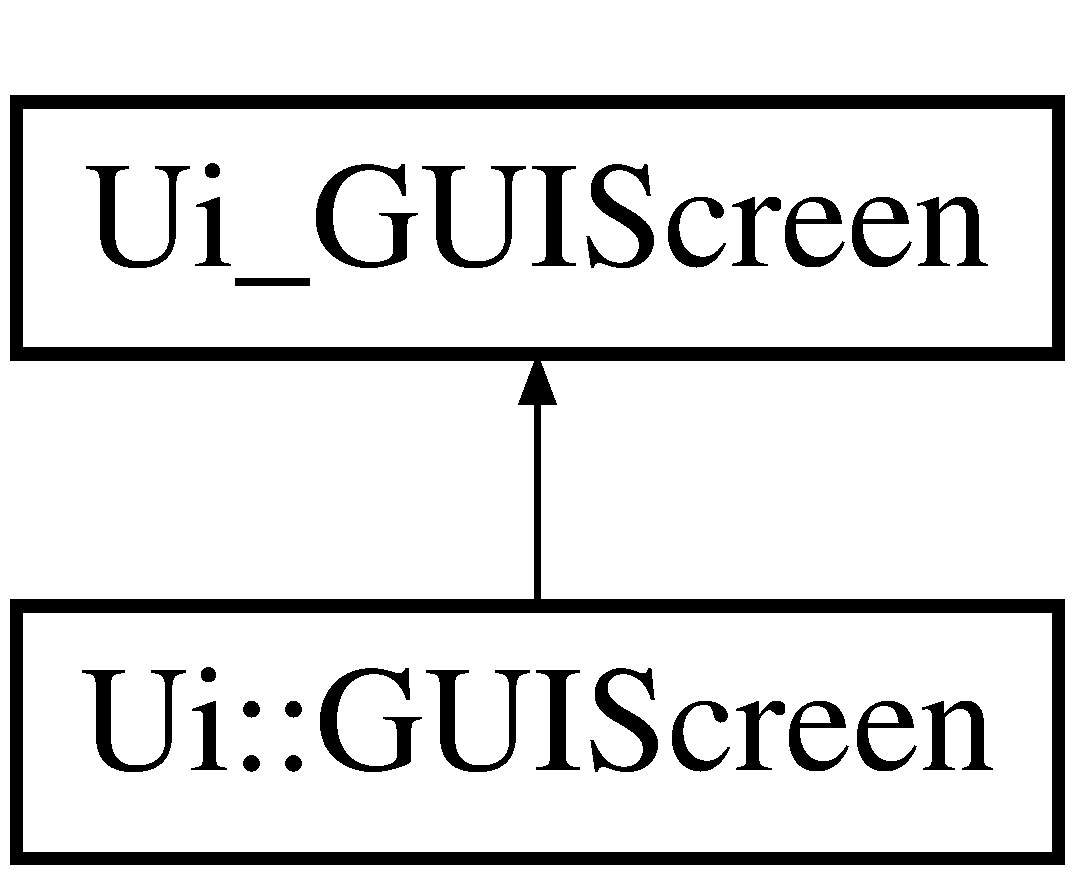
\includegraphics[height=2.000000cm]{class_ui___g_u_i_screen}
\end{center}
\end{figure}
\subsection*{Public Member Functions}
\begin{DoxyCompactItemize}
\item 
\mbox{\Hypertarget{class_ui___g_u_i_screen_a7ca728c75177f9a79e380e0635dfd24a}\label{class_ui___g_u_i_screen_a7ca728c75177f9a79e380e0635dfd24a}} 
void {\bfseries setup\+Ui} (Q\+Widget $\ast$\hyperlink{class_g_u_i_screen}{G\+U\+I\+Screen})
\item 
\mbox{\Hypertarget{class_ui___g_u_i_screen_aab74d6cd64fdddbd9e5cfd77fbb96871}\label{class_ui___g_u_i_screen_aab74d6cd64fdddbd9e5cfd77fbb96871}} 
void {\bfseries retranslate\+Ui} (Q\+Widget $\ast$\hyperlink{class_g_u_i_screen}{G\+U\+I\+Screen})
\end{DoxyCompactItemize}
\subsection*{Public Attributes}
\begin{DoxyCompactItemize}
\item 
\mbox{\Hypertarget{class_ui___g_u_i_screen_a74084d36085bfd9e2cd539a7fc1d6f15}\label{class_ui___g_u_i_screen_a74084d36085bfd9e2cd539a7fc1d6f15}} 
Q\+Stacked\+Widget $\ast$ {\bfseries stacked\+Widget}
\item 
\mbox{\Hypertarget{class_ui___g_u_i_screen_a882716dcde30f9a4d69f8fb88c9ab810}\label{class_ui___g_u_i_screen_a882716dcde30f9a4d69f8fb88c9ab810}} 
Q\+Widget $\ast$ {\bfseries user\+Name\+Screen}
\item 
\mbox{\Hypertarget{class_ui___g_u_i_screen_a71bde7465a0209f24893aa2145e8c7db}\label{class_ui___g_u_i_screen_a71bde7465a0209f24893aa2145e8c7db}} 
Q\+Label $\ast$ {\bfseries Mine\+Sweeper\+Title}
\item 
\mbox{\Hypertarget{class_ui___g_u_i_screen_a09f861ef3cbb1731602c68c254d81bad}\label{class_ui___g_u_i_screen_a09f861ef3cbb1731602c68c254d81bad}} 
Q\+Push\+Button $\ast$ {\bfseries play\+Button}
\item 
\mbox{\Hypertarget{class_ui___g_u_i_screen_a972e419ef466b6878129989a2cf70f23}\label{class_ui___g_u_i_screen_a972e419ef466b6878129989a2cf70f23}} 
Q\+Widget $\ast$ {\bfseries layout\+Widget}
\item 
\mbox{\Hypertarget{class_ui___g_u_i_screen_af1e6df275fe1d51b54440e6ebc340f41}\label{class_ui___g_u_i_screen_af1e6df275fe1d51b54440e6ebc340f41}} 
Q\+H\+Box\+Layout $\ast$ {\bfseries horizontal\+Layout\+\_\+5}
\item 
\mbox{\Hypertarget{class_ui___g_u_i_screen_a2c98bc4adad660e9040cbfb6a1b38e2f}\label{class_ui___g_u_i_screen_a2c98bc4adad660e9040cbfb6a1b38e2f}} 
Q\+Label $\ast$ {\bfseries username\+Title}
\item 
\mbox{\Hypertarget{class_ui___g_u_i_screen_a5cc646e697d52864086568834da89c4e}\label{class_ui___g_u_i_screen_a5cc646e697d52864086568834da89c4e}} 
Q\+Spacer\+Item $\ast$ {\bfseries horizontal\+Spacer\+\_\+7}
\item 
\mbox{\Hypertarget{class_ui___g_u_i_screen_a8328aa2d8960823a776571e9a270a244}\label{class_ui___g_u_i_screen_a8328aa2d8960823a776571e9a270a244}} 
Q\+Line\+Edit $\ast$ {\bfseries username\+Input}
\item 
\mbox{\Hypertarget{class_ui___g_u_i_screen_a4152533ad34cd99ae01defc6757b8d9f}\label{class_ui___g_u_i_screen_a4152533ad34cd99ae01defc6757b8d9f}} 
Q\+Widget $\ast$ {\bfseries init\+Screen}
\item 
\mbox{\Hypertarget{class_ui___g_u_i_screen_afdbf3e0c3ee19a9b10b2f03bc65fc63b}\label{class_ui___g_u_i_screen_afdbf3e0c3ee19a9b10b2f03bc65fc63b}} 
Q\+Label $\ast$ {\bfseries game\+Title}
\item 
\mbox{\Hypertarget{class_ui___g_u_i_screen_ae787caab477bd13bec24ad1c3f50562a}\label{class_ui___g_u_i_screen_ae787caab477bd13bec24ad1c3f50562a}} 
Q\+Label $\ast$ {\bfseries default\+Game\+Title}
\item 
\mbox{\Hypertarget{class_ui___g_u_i_screen_adbd8d94d269d0dccd1009198380f0a0d}\label{class_ui___g_u_i_screen_adbd8d94d269d0dccd1009198380f0a0d}} 
Q\+Push\+Button $\ast$ {\bfseries default\+Game\+Button}
\item 
\mbox{\Hypertarget{class_ui___g_u_i_screen_a60c017496a306bae989fe856b82f92f2}\label{class_ui___g_u_i_screen_a60c017496a306bae989fe856b82f92f2}} 
Q\+Frame $\ast$ {\bfseries line}
\item 
\mbox{\Hypertarget{class_ui___g_u_i_screen_a26f89fe8fab356cdf86f95020eda1782}\label{class_ui___g_u_i_screen_a26f89fe8fab356cdf86f95020eda1782}} 
Q\+Label $\ast$ {\bfseries personnalized\+Game\+Title}
\item 
\mbox{\Hypertarget{class_ui___g_u_i_screen_a4a0176e792088d9a27ea0396e31b3f1f}\label{class_ui___g_u_i_screen_a4a0176e792088d9a27ea0396e31b3f1f}} 
Q\+Label $\ast$ {\bfseries label\+\_\+3}
\item 
\mbox{\Hypertarget{class_ui___g_u_i_screen_a0575158e303a368dbda7957d7cb24105}\label{class_ui___g_u_i_screen_a0575158e303a368dbda7957d7cb24105}} 
Q\+Label $\ast$ {\bfseries label\+\_\+4}
\item 
\mbox{\Hypertarget{class_ui___g_u_i_screen_a3f1ed9b32c050b2244d389306583c3e5}\label{class_ui___g_u_i_screen_a3f1ed9b32c050b2244d389306583c3e5}} 
Q\+Check\+Box $\ast$ {\bfseries default\+Nb\+Bomb}
\item 
\mbox{\Hypertarget{class_ui___g_u_i_screen_a0ece335a6fa42b019ee3d82d30bb5d75}\label{class_ui___g_u_i_screen_a0ece335a6fa42b019ee3d82d30bb5d75}} 
Q\+Push\+Button $\ast$ {\bfseries personnalized\+Game\+Button}
\item 
\mbox{\Hypertarget{class_ui___g_u_i_screen_a217005eb6e8b1cd7c00a8986ff732e05}\label{class_ui___g_u_i_screen_a217005eb6e8b1cd7c00a8986ff732e05}} 
Q\+Frame $\ast$ {\bfseries line\+\_\+2}
\item 
\mbox{\Hypertarget{class_ui___g_u_i_screen_a6e8c669ced922fc71a0f9223d74cba40}\label{class_ui___g_u_i_screen_a6e8c669ced922fc71a0f9223d74cba40}} 
Q\+Push\+Button $\ast$ {\bfseries hall\+Of\+Fame\+Button}
\item 
\mbox{\Hypertarget{class_ui___g_u_i_screen_a3992ca826a0b2beb8e345c74ba712e3b}\label{class_ui___g_u_i_screen_a3992ca826a0b2beb8e345c74ba712e3b}} 
Q\+Push\+Button $\ast$ {\bfseries quit\+Button}
\item 
\mbox{\Hypertarget{class_ui___g_u_i_screen_a4579f4bb534fba939d2f3d6fcb4e43d8}\label{class_ui___g_u_i_screen_a4579f4bb534fba939d2f3d6fcb4e43d8}} 
Q\+Widget $\ast$ {\bfseries layout\+Widget1}
\item 
\mbox{\Hypertarget{class_ui___g_u_i_screen_acc3763901501986a37f65d4e4e1942be}\label{class_ui___g_u_i_screen_acc3763901501986a37f65d4e4e1942be}} 
Q\+H\+Box\+Layout $\ast$ {\bfseries horizontal\+Layout}
\item 
\mbox{\Hypertarget{class_ui___g_u_i_screen_ad4f1300f8f325f176f6c0cb5a6200e9e}\label{class_ui___g_u_i_screen_ad4f1300f8f325f176f6c0cb5a6200e9e}} 
Q\+Label $\ast$ {\bfseries line\+Title}
\item 
\mbox{\Hypertarget{class_ui___g_u_i_screen_a4c55d4aa1d22af5d8d231a8ddac4b47f}\label{class_ui___g_u_i_screen_a4c55d4aa1d22af5d8d231a8ddac4b47f}} 
Q\+Spacer\+Item $\ast$ {\bfseries horizontal\+Spacer}
\item 
\mbox{\Hypertarget{class_ui___g_u_i_screen_a85fef5091acd271045cc8e565aaddcf7}\label{class_ui___g_u_i_screen_a85fef5091acd271045cc8e565aaddcf7}} 
Q\+Line\+Edit $\ast$ {\bfseries nb\+Line\+Input}
\item 
\mbox{\Hypertarget{class_ui___g_u_i_screen_aa001e60153cff4ef60045e2af3a2a553}\label{class_ui___g_u_i_screen_aa001e60153cff4ef60045e2af3a2a553}} 
Q\+Widget $\ast$ {\bfseries layout\+Widget2}
\item 
\mbox{\Hypertarget{class_ui___g_u_i_screen_a093961b6a75aa53b1121abdcbdf8964a}\label{class_ui___g_u_i_screen_a093961b6a75aa53b1121abdcbdf8964a}} 
Q\+H\+Box\+Layout $\ast$ {\bfseries horizontal\+Layout\+\_\+2}
\item 
\mbox{\Hypertarget{class_ui___g_u_i_screen_a032b2504f99590615a546a9b93a77dbe}\label{class_ui___g_u_i_screen_a032b2504f99590615a546a9b93a77dbe}} 
Q\+Label $\ast$ {\bfseries label\+\_\+2}
\item 
\mbox{\Hypertarget{class_ui___g_u_i_screen_a8c085a40466cbf70f075658982d2fe44}\label{class_ui___g_u_i_screen_a8c085a40466cbf70f075658982d2fe44}} 
Q\+Spacer\+Item $\ast$ {\bfseries horizontal\+Spacer\+\_\+2}
\item 
\mbox{\Hypertarget{class_ui___g_u_i_screen_ac8400b5483ee71ba6ae9400e54080d3e}\label{class_ui___g_u_i_screen_ac8400b5483ee71ba6ae9400e54080d3e}} 
Q\+Line\+Edit $\ast$ {\bfseries nb\+Column\+Input}
\item 
\mbox{\Hypertarget{class_ui___g_u_i_screen_a0010a829260abb7e63507473dc7cdb39}\label{class_ui___g_u_i_screen_a0010a829260abb7e63507473dc7cdb39}} 
Q\+Widget $\ast$ {\bfseries layout\+Widget3}
\item 
\mbox{\Hypertarget{class_ui___g_u_i_screen_afd4fe60919d7fdfd926d74498d3f5053}\label{class_ui___g_u_i_screen_afd4fe60919d7fdfd926d74498d3f5053}} 
Q\+H\+Box\+Layout $\ast$ {\bfseries horizontal\+Layout\+\_\+3}
\item 
\mbox{\Hypertarget{class_ui___g_u_i_screen_ac88621fb5a3866496d82e7ef6fb17083}\label{class_ui___g_u_i_screen_ac88621fb5a3866496d82e7ef6fb17083}} 
Q\+Label $\ast$ {\bfseries label}
\item 
\mbox{\Hypertarget{class_ui___g_u_i_screen_ad3c29fc34dcf9202a29710b21e31346c}\label{class_ui___g_u_i_screen_ad3c29fc34dcf9202a29710b21e31346c}} 
Q\+Spacer\+Item $\ast$ {\bfseries horizontal\+Spacer\+\_\+3}
\item 
\mbox{\Hypertarget{class_ui___g_u_i_screen_aad20cca43952251c38166436d740d9da}\label{class_ui___g_u_i_screen_aad20cca43952251c38166436d740d9da}} 
Q\+Line\+Edit $\ast$ {\bfseries bomb\+Input}
\item 
\mbox{\Hypertarget{class_ui___g_u_i_screen_aa6e99af948e2320c44ef8422fc7437f7}\label{class_ui___g_u_i_screen_aa6e99af948e2320c44ef8422fc7437f7}} 
Q\+Spacer\+Item $\ast$ {\bfseries horizontal\+Spacer\+\_\+4}
\item 
\mbox{\Hypertarget{class_ui___g_u_i_screen_afb29c01978a7bf3bee4ac4b31bbbdd4d}\label{class_ui___g_u_i_screen_afb29c01978a7bf3bee4ac4b31bbbdd4d}} 
Q\+Combo\+Box $\ast$ {\bfseries bombs\+Unit}
\item 
\mbox{\Hypertarget{class_ui___g_u_i_screen_afdeabcfeaff402fa17adda362528090f}\label{class_ui___g_u_i_screen_afdeabcfeaff402fa17adda362528090f}} 
Q\+Widget $\ast$ {\bfseries play\+Screen}
\item 
\mbox{\Hypertarget{class_ui___g_u_i_screen_a7495562e52aa39544c9ab04bf6d92d6f}\label{class_ui___g_u_i_screen_a7495562e52aa39544c9ab04bf6d92d6f}} 
Q\+L\+C\+D\+Number $\ast$ {\bfseries timer}
\item 
\mbox{\Hypertarget{class_ui___g_u_i_screen_a3b518d99653dde012576055447cd089f}\label{class_ui___g_u_i_screen_a3b518d99653dde012576055447cd089f}} 
Q\+Widget $\ast$ {\bfseries frame}
\item 
\mbox{\Hypertarget{class_ui___g_u_i_screen_ac91e777d26fda9a4cca5d0298332e6af}\label{class_ui___g_u_i_screen_ac91e777d26fda9a4cca5d0298332e6af}} 
Q\+Push\+Button $\ast$ {\bfseries exit\+Button}
\item 
\mbox{\Hypertarget{class_ui___g_u_i_screen_ae7d2cded72db2bb5a3aa05b19ad483eb}\label{class_ui___g_u_i_screen_ae7d2cded72db2bb5a3aa05b19ad483eb}} 
Q\+Push\+Button $\ast$ {\bfseries give\+Up\+Button}
\item 
\mbox{\Hypertarget{class_ui___g_u_i_screen_ae33255c2e964db247429319a263d4c5f}\label{class_ui___g_u_i_screen_ae33255c2e964db247429319a263d4c5f}} 
Q\+Push\+Button $\ast$ {\bfseries bonus\+Button}
\item 
\mbox{\Hypertarget{class_ui___g_u_i_screen_a6dce1285327e3302647d0260461eae95}\label{class_ui___g_u_i_screen_a6dce1285327e3302647d0260461eae95}} 
Q\+L\+C\+D\+Number $\ast$ {\bfseries bomb\+Counter}
\item 
\mbox{\Hypertarget{class_ui___g_u_i_screen_af3415b1647ecfa88deeebdff7d8a8b66}\label{class_ui___g_u_i_screen_af3415b1647ecfa88deeebdff7d8a8b66}} 
Q\+Label $\ast$ {\bfseries label\+\_\+6}
\item 
\mbox{\Hypertarget{class_ui___g_u_i_screen_a5e90716987a4e915eae2f02877475374}\label{class_ui___g_u_i_screen_a5e90716987a4e915eae2f02877475374}} 
Q\+Label $\ast$ {\bfseries label\+\_\+7}
\item 
\mbox{\Hypertarget{class_ui___g_u_i_screen_a959929e050a49c901d036ce8816a7f4c}\label{class_ui___g_u_i_screen_a959929e050a49c901d036ce8816a7f4c}} 
Q\+Label $\ast$ {\bfseries help}
\item 
\mbox{\Hypertarget{class_ui___g_u_i_screen_ae3e566a2787c8b72c253528b1a1a56d8}\label{class_ui___g_u_i_screen_ae3e566a2787c8b72c253528b1a1a56d8}} 
Q\+Widget $\ast$ {\bfseries stat\+Screen}
\item 
\mbox{\Hypertarget{class_ui___g_u_i_screen_af669025817754e781a84b789e2770e56}\label{class_ui___g_u_i_screen_af669025817754e781a84b789e2770e56}} 
Q\+Table\+Widget $\ast$ {\bfseries scores\+Board}
\item 
\mbox{\Hypertarget{class_ui___g_u_i_screen_a2fcfcb0bc118a1eb5b8b832807cf31bb}\label{class_ui___g_u_i_screen_a2fcfcb0bc118a1eb5b8b832807cf31bb}} 
Q\+Widget $\ast$ {\bfseries layout\+Widget4}
\item 
\mbox{\Hypertarget{class_ui___g_u_i_screen_a77a007efc2b316fa01d12790ae0b21b6}\label{class_ui___g_u_i_screen_a77a007efc2b316fa01d12790ae0b21b6}} 
Q\+H\+Box\+Layout $\ast$ {\bfseries horizontal\+Layout\+\_\+4}
\item 
\mbox{\Hypertarget{class_ui___g_u_i_screen_a2d07d06594a800c040b4b04f4fd6818a}\label{class_ui___g_u_i_screen_a2d07d06594a800c040b4b04f4fd6818a}} 
Q\+Label $\ast$ {\bfseries label\+\_\+5}
\item 
\mbox{\Hypertarget{class_ui___g_u_i_screen_a31c7bbf132e097882bb4127f300f8aab}\label{class_ui___g_u_i_screen_a31c7bbf132e097882bb4127f300f8aab}} 
Q\+Spacer\+Item $\ast$ {\bfseries horizontal\+Spacer\+\_\+5}
\item 
\mbox{\Hypertarget{class_ui___g_u_i_screen_a55537d63eb5fbd3185eacc1151b1c1ff}\label{class_ui___g_u_i_screen_a55537d63eb5fbd3185eacc1151b1c1ff}} 
Q\+Combo\+Box $\ast$ {\bfseries board\+Type\+Box}
\item 
\mbox{\Hypertarget{class_ui___g_u_i_screen_aa9621b0257f383b893f1fa418e85ce49}\label{class_ui___g_u_i_screen_aa9621b0257f383b893f1fa418e85ce49}} 
Q\+Spacer\+Item $\ast$ {\bfseries horizontal\+Spacer\+\_\+6}
\item 
\mbox{\Hypertarget{class_ui___g_u_i_screen_af0591d21d68d848c16efb1b74e27a6d5}\label{class_ui___g_u_i_screen_af0591d21d68d848c16efb1b74e27a6d5}} 
Q\+Push\+Button $\ast$ {\bfseries print\+Score\+Button}
\item 
\mbox{\Hypertarget{class_ui___g_u_i_screen_a06c7d37afb6b87d408a4152b9fd71577}\label{class_ui___g_u_i_screen_a06c7d37afb6b87d408a4152b9fd71577}} 
Q\+Push\+Button $\ast$ {\bfseries to\+Init\+Screen\+Button}
\end{DoxyCompactItemize}


\subsection{Detailed Description}


Definition at line 32 of file ui\+\_\+guiscreen.\+h.



The documentation for this class was generated from the following file\+:\begin{DoxyCompactItemize}
\item 
Application/ui\+\_\+guiscreen.\+h\end{DoxyCompactItemize}

\hypertarget{class_ui__start_screen}{}\section{Ui\+\_\+start\+Screen Class Reference}
\label{class_ui__start_screen}\index{Ui\+\_\+start\+Screen@{Ui\+\_\+start\+Screen}}
Inheritance diagram for Ui\+\_\+start\+Screen\+:\begin{figure}[H]
\begin{center}
\leavevmode
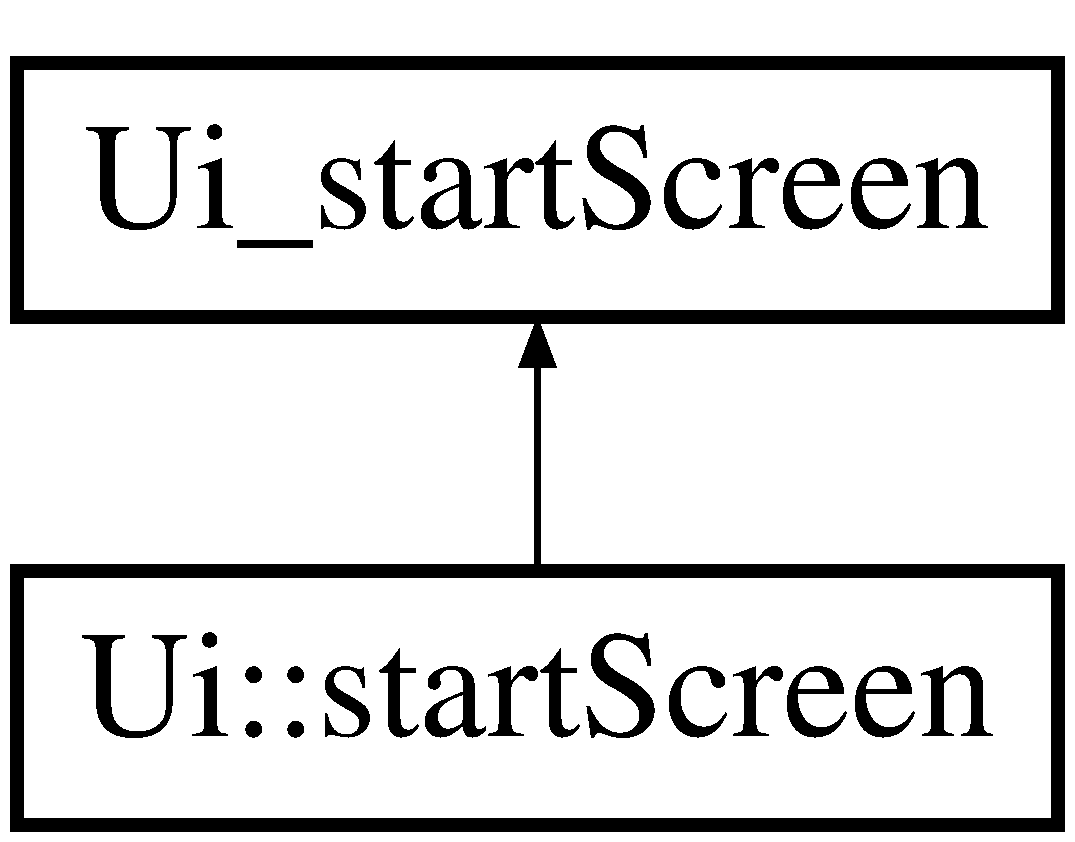
\includegraphics[height=2.000000cm]{class_ui__start_screen}
\end{center}
\end{figure}
\subsection*{Public Member Functions}
\begin{DoxyCompactItemize}
\item 
\mbox{\Hypertarget{class_ui__start_screen_a65bb6043706a33b91a8c3c54db5f30c7}\label{class_ui__start_screen_a65bb6043706a33b91a8c3c54db5f30c7}} 
void {\bfseries setup\+Ui} (Q\+Widget $\ast$start\+Screen)
\item 
\mbox{\Hypertarget{class_ui__start_screen_a02b30ff925cdf7a4403b57e9fe3a41ac}\label{class_ui__start_screen_a02b30ff925cdf7a4403b57e9fe3a41ac}} 
void {\bfseries retranslate\+Ui} (Q\+Widget $\ast$start\+Screen)
\end{DoxyCompactItemize}
\subsection*{Public Attributes}
\begin{DoxyCompactItemize}
\item 
\mbox{\Hypertarget{class_ui__start_screen_a6d794d4aff2d4c46ca2ddfd106043b49}\label{class_ui__start_screen_a6d794d4aff2d4c46ca2ddfd106043b49}} 
Q\+Stacked\+Widget $\ast$ {\bfseries stacked\+Widget}
\item 
\mbox{\Hypertarget{class_ui__start_screen_a8c1ca92c5a46be9cdcfb8e3decfa9cc1}\label{class_ui__start_screen_a8c1ca92c5a46be9cdcfb8e3decfa9cc1}} 
Q\+Widget $\ast$ {\bfseries page}
\item 
\mbox{\Hypertarget{class_ui__start_screen_a8f8bd56ba450567296c931ab4f0a1105}\label{class_ui__start_screen_a8f8bd56ba450567296c931ab4f0a1105}} 
Q\+Widget $\ast$ {\bfseries layout\+Widget}
\item 
\mbox{\Hypertarget{class_ui__start_screen_a2781a818aec229be157059afe8ac7813}\label{class_ui__start_screen_a2781a818aec229be157059afe8ac7813}} 
Q\+V\+Box\+Layout $\ast$ {\bfseries vertical\+Layout\+\_\+3}
\item 
\mbox{\Hypertarget{class_ui__start_screen_a5ac50db9fc432fe7ef74f90b59d34ad7}\label{class_ui__start_screen_a5ac50db9fc432fe7ef74f90b59d34ad7}} 
Q\+Label $\ast$ {\bfseries label}
\item 
\mbox{\Hypertarget{class_ui__start_screen_ada51cd3dc974716cc83b4b658c1a45a8}\label{class_ui__start_screen_ada51cd3dc974716cc83b4b658c1a45a8}} 
Q\+V\+Box\+Layout $\ast$ {\bfseries vertical\+Layout}
\item 
\mbox{\Hypertarget{class_ui__start_screen_a915e1f2f5f8103f69038a85d76e821b7}\label{class_ui__start_screen_a915e1f2f5f8103f69038a85d76e821b7}} 
Q\+Label $\ast$ {\bfseries label\+\_\+2}
\item 
\mbox{\Hypertarget{class_ui__start_screen_a6e1b1916e66d2163336b15d47d452359}\label{class_ui__start_screen_a6e1b1916e66d2163336b15d47d452359}} 
Q\+Push\+Button $\ast$ {\bfseries game\+Default\+Btn}
\item 
\mbox{\Hypertarget{class_ui__start_screen_a6d08679c4f927ff0c057f439d3f759d2}\label{class_ui__start_screen_a6d08679c4f927ff0c057f439d3f759d2}} 
Q\+Frame $\ast$ {\bfseries line}
\item 
\mbox{\Hypertarget{class_ui__start_screen_a0905f2e7439e1040e45c229042852297}\label{class_ui__start_screen_a0905f2e7439e1040e45c229042852297}} 
Q\+V\+Box\+Layout $\ast$ {\bfseries vertical\+Layout\+\_\+2}
\item 
\mbox{\Hypertarget{class_ui__start_screen_a4beb6791e4313b0fa9397f2b3f7346e3}\label{class_ui__start_screen_a4beb6791e4313b0fa9397f2b3f7346e3}} 
Q\+Label $\ast$ {\bfseries label\+\_\+3}
\item 
\mbox{\Hypertarget{class_ui__start_screen_a993ff5ec1b6052e05ea780115d278911}\label{class_ui__start_screen_a993ff5ec1b6052e05ea780115d278911}} 
Q\+H\+Box\+Layout $\ast$ {\bfseries horizontal\+Layout}
\item 
\mbox{\Hypertarget{class_ui__start_screen_a1b4251346abca505c771e369ab711d04}\label{class_ui__start_screen_a1b4251346abca505c771e369ab711d04}} 
Q\+Label $\ast$ {\bfseries label\+\_\+4}
\item 
\mbox{\Hypertarget{class_ui__start_screen_a19865f7bfe5be1e9ea188e5fb3693453}\label{class_ui__start_screen_a19865f7bfe5be1e9ea188e5fb3693453}} 
Q\+Line\+Edit $\ast$ {\bfseries nb\+Row\+Tf}
\item 
\mbox{\Hypertarget{class_ui__start_screen_a3fc9f2185dacce0db9963e47fa6fcf7f}\label{class_ui__start_screen_a3fc9f2185dacce0db9963e47fa6fcf7f}} 
Q\+H\+Box\+Layout $\ast$ {\bfseries horizontal\+Layout\+\_\+2}
\item 
\mbox{\Hypertarget{class_ui__start_screen_a9f1407adc072c8e6eca670f246e04604}\label{class_ui__start_screen_a9f1407adc072c8e6eca670f246e04604}} 
Q\+Label $\ast$ {\bfseries label\+\_\+5}
\item 
\mbox{\Hypertarget{class_ui__start_screen_a9ad6ae29ea77971e55b836768c09d2c3}\label{class_ui__start_screen_a9ad6ae29ea77971e55b836768c09d2c3}} 
Q\+Line\+Edit $\ast$ {\bfseries nb\+Col\+Tf}
\item 
\mbox{\Hypertarget{class_ui__start_screen_ac90b36798ee122eaee2bea171f31b5f6}\label{class_ui__start_screen_ac90b36798ee122eaee2bea171f31b5f6}} 
Q\+H\+Box\+Layout $\ast$ {\bfseries horizontal\+Layout\+\_\+3}
\item 
\mbox{\Hypertarget{class_ui__start_screen_a182e707dc6db663995371ab5ff1c5a30}\label{class_ui__start_screen_a182e707dc6db663995371ab5ff1c5a30}} 
Q\+Label $\ast$ {\bfseries label\+\_\+6}
\item 
\mbox{\Hypertarget{class_ui__start_screen_acc1600d78680f2f64fa8d9c74f34746e}\label{class_ui__start_screen_acc1600d78680f2f64fa8d9c74f34746e}} 
Q\+Line\+Edit $\ast$ {\bfseries nb\+Bomb\+Tf}
\item 
\mbox{\Hypertarget{class_ui__start_screen_ad865e54b0f68688326c930d8f99b7953}\label{class_ui__start_screen_ad865e54b0f68688326c930d8f99b7953}} 
Q\+Combo\+Box $\ast$ {\bfseries bomb\+Unit}
\item 
\mbox{\Hypertarget{class_ui__start_screen_a8abc877cc6de75d4055aecec623538d7}\label{class_ui__start_screen_a8abc877cc6de75d4055aecec623538d7}} 
Q\+Label $\ast$ {\bfseries label\+\_\+7}
\item 
\mbox{\Hypertarget{class_ui__start_screen_ac6431132ee9656b4df6483c4d65e9293}\label{class_ui__start_screen_ac6431132ee9656b4df6483c4d65e9293}} 
Q\+Label $\ast$ {\bfseries label\+\_\+8}
\item 
\mbox{\Hypertarget{class_ui__start_screen_a748c88ee957f7bab3779c8b23e33e0f6}\label{class_ui__start_screen_a748c88ee957f7bab3779c8b23e33e0f6}} 
Q\+Check\+Box $\ast$ {\bfseries bomb\+Default}
\item 
\mbox{\Hypertarget{class_ui__start_screen_abe3209291201937f25c7f74849c968d7}\label{class_ui__start_screen_abe3209291201937f25c7f74849c968d7}} 
Q\+Push\+Button $\ast$ {\bfseries game\+Custom\+Btn}
\item 
\mbox{\Hypertarget{class_ui__start_screen_ab172fa5ae48a27889bbf86a9a0ee4f41}\label{class_ui__start_screen_ab172fa5ae48a27889bbf86a9a0ee4f41}} 
Q\+Widget $\ast$ {\bfseries page\+\_\+2}
\item 
\mbox{\Hypertarget{class_ui__start_screen_a222548ace3833bf639d27efbb3cafbd2}\label{class_ui__start_screen_a222548ace3833bf639d27efbb3cafbd2}} 
Q\+L\+C\+D\+Number $\ast$ {\bfseries lcd\+Number}
\item 
\mbox{\Hypertarget{class_ui__start_screen_ac0c1a6098adbc0301d4b2763189b073f}\label{class_ui__start_screen_ac0c1a6098adbc0301d4b2763189b073f}} 
Q\+Widget $\ast$ {\bfseries vertical\+Layout\+Widget}
\item 
\mbox{\Hypertarget{class_ui__start_screen_a8a862f9ef22b6ff4c720a627ba3e4a8e}\label{class_ui__start_screen_a8a862f9ef22b6ff4c720a627ba3e4a8e}} 
Q\+V\+Box\+Layout $\ast$ {\bfseries container\+Case}
\item 
\mbox{\Hypertarget{class_ui__start_screen_a709d08547be894f11902a5f62dddf545}\label{class_ui__start_screen_a709d08547be894f11902a5f62dddf545}} 
Q\+Widget $\ast$ {\bfseries layout\+Widget1}
\item 
\mbox{\Hypertarget{class_ui__start_screen_aa05174af6deedf54ba54eb7296599764}\label{class_ui__start_screen_aa05174af6deedf54ba54eb7296599764}} 
Q\+H\+Box\+Layout $\ast$ {\bfseries horizontal\+Layout\+\_\+4}
\item 
\mbox{\Hypertarget{class_ui__start_screen_a6389fdd44c964fb70229ddd3b2e0945d}\label{class_ui__start_screen_a6389fdd44c964fb70229ddd3b2e0945d}} 
Q\+Push\+Button $\ast$ {\bfseries new\+Game\+Btn}
\item 
\mbox{\Hypertarget{class_ui__start_screen_adee432c8c443937042ec38ff3b55cec3}\label{class_ui__start_screen_adee432c8c443937042ec38ff3b55cec3}} 
Q\+Frame $\ast$ {\bfseries line\+\_\+2}
\item 
\mbox{\Hypertarget{class_ui__start_screen_ab3ab96128b6f39523da12c56f6f887b0}\label{class_ui__start_screen_ab3ab96128b6f39523da12c56f6f887b0}} 
Q\+Push\+Button $\ast$ {\bfseries stat\+Btn}
\end{DoxyCompactItemize}


\subsection{Detailed Description}


Definition at line 31 of file ui\+\_\+startscreen.\+h.



The documentation for this class was generated from the following file\+:\begin{DoxyCompactItemize}
\item 
Application/ui\+\_\+startscreen.\+h\end{DoxyCompactItemize}

\hypertarget{class_catch_1_1_values_generator}{}\section{Catch\+:\+:Values\+Generator$<$ T $>$ Class Template Reference}
\label{class_catch_1_1_values_generator}\index{Catch\+::\+Values\+Generator$<$ T $>$@{Catch\+::\+Values\+Generator$<$ T $>$}}
Inheritance diagram for Catch\+:\+:Values\+Generator$<$ T $>$\+:\begin{figure}[H]
\begin{center}
\leavevmode
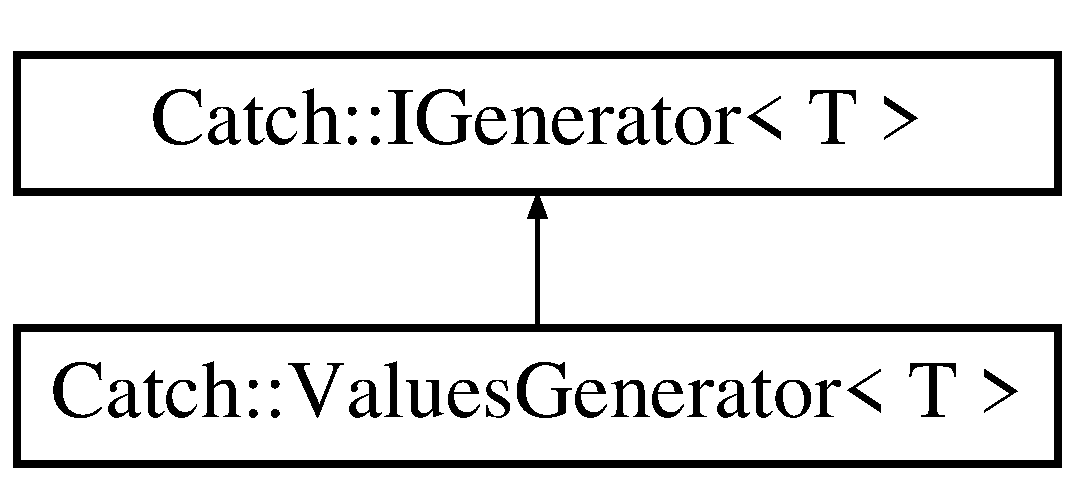
\includegraphics[height=2.000000cm]{class_catch_1_1_values_generator}
\end{center}
\end{figure}
\subsection*{Public Member Functions}
\begin{DoxyCompactItemize}
\item 
\mbox{\Hypertarget{class_catch_1_1_values_generator_a8412c8ce5d9d4fc6ff06d5246d56d538}\label{class_catch_1_1_values_generator_a8412c8ce5d9d4fc6ff06d5246d56d538}} 
void {\bfseries add} (T value)
\item 
\mbox{\Hypertarget{class_catch_1_1_values_generator_a9674c8b70d562d2d68154de92dd1810a}\label{class_catch_1_1_values_generator_a9674c8b70d562d2d68154de92dd1810a}} 
virtual T {\bfseries get\+Value} (\textbf{ std\+::size\+\_\+t} index) const
\item 
\mbox{\Hypertarget{class_catch_1_1_values_generator_a9aa5b140ee502975cf35115e534ab771}\label{class_catch_1_1_values_generator_a9aa5b140ee502975cf35115e534ab771}} 
virtual \textbf{ std\+::size\+\_\+t} {\bfseries size} () const
\end{DoxyCompactItemize}


\subsection{Detailed Description}
\subsubsection*{template$<$typename T$>$\newline
class Catch\+::\+Values\+Generator$<$ T $>$}



Definition at line 2327 of file catch.\+hpp.



The documentation for this class was generated from the following file\+:\begin{DoxyCompactItemize}
\item 
Tests/catch.\+hpp\end{DoxyCompactItemize}

\hypertarget{class_view}{}\section{View Class Reference}
\label{class_view}\index{View@{View}}


The \hyperlink{class_view}{View} class This class represents the view of the \hyperlink{class_game}{Game}. It handles all the thing that must be displayed such as the board, the different messages for the player.  




{\ttfamily \#include $<$view.\+h$>$}

\subsection*{Public Member Functions}
\begin{DoxyCompactItemize}
\item 
\hyperlink{class_view_a7c91b725a55a7843fc628e29d85f53a2}{View} (\hyperlink{class_game}{Game} $\ast$game)
\begin{DoxyCompactList}\small\item\em \hyperlink{class_view}{View} Creates an instance of the class with a predefined \hyperlink{class_game}{Game}. \end{DoxyCompactList}\item 
\mbox{\Hypertarget{class_view_a44ad60a768422d3fa8fbd7576950080a}\label{class_view_a44ad60a768422d3fa8fbd7576950080a}} 
\hyperlink{class_view_a44ad60a768422d3fa8fbd7576950080a}{View} ()
\begin{DoxyCompactList}\small\item\em \hyperlink{class_view}{View} Creates an instance of the class from nothing. \end{DoxyCompactList}\item 
\mbox{\Hypertarget{class_view_ad0dc854db9aabbea98a334dec89f785c}\label{class_view_ad0dc854db9aabbea98a334dec89f785c}} 
\hyperlink{class_view_ad0dc854db9aabbea98a334dec89f785c}{$\sim$\+View} ()
\begin{DoxyCompactList}\small\item\em the destructor. Deletes all the elements of the class that need to be deleted. \end{DoxyCompactList}\item 
void \hyperlink{class_view_a3f47f684fa69af930056c56e4d559c7d}{set\+Game} (\hyperlink{class_game}{Game} $\ast$game)
\begin{DoxyCompactList}\small\item\em set\+Game Set the attribute game\+\_\+ with the value of the \hyperlink{class_game}{Game} in parameter. \end{DoxyCompactList}\item 
void \hyperlink{class_view_ac837e4c674546a4bfccbb58250a81f6b}{set\+Controller} (\hyperlink{class_controller}{Controller} $\ast$controller)
\begin{DoxyCompactList}\small\item\em set\+Controller Set the attribute controller\+\_\+ with the value of the \hyperlink{class_controller}{Controller} in parameter. \end{DoxyCompactList}\item 
\mbox{\Hypertarget{class_view_ab5964dab1ea4bf6d23513e21a212f00a}\label{class_view_ab5964dab1ea4bf6d23513e21a212f00a}} 
void \hyperlink{class_view_ab5964dab1ea4bf6d23513e21a212f00a}{print\+Board} ()
\begin{DoxyCompactList}\small\item\em print\+Board Displays the board. \end{DoxyCompactList}\item 
bool \hyperlink{class_view_aad0487a7cc70e7e03ce8d0dc39c570c4}{is\+Play\+Command} (\textbf{ std\+::vector}$<$ \textbf{ string} $>$ my\+Command)
\begin{DoxyCompactList}\small\item\em is\+Play\+Command Indicates if the first element of the vector my\+Command is \char`\"{}\+P\+L\+A\+Y\char`\"{}. \end{DoxyCompactList}\item 
bool \hyperlink{class_view_a26d427abb478561381207ed8d76d84c4}{is\+Flag\+Command} (\textbf{ std\+::vector}$<$ \textbf{ string} $>$ my\+Command)
\begin{DoxyCompactList}\small\item\em is\+Flag\+Command Indicates if the first element of the vector my\+Command is \char`\"{}\+F\+L\+A\+G\char`\"{}. \end{DoxyCompactList}\item 
bool \hyperlink{class_view_ac3a7757f7c123e73569e3b9bcf89df86}{is\+Exit\+Command} (\textbf{ std\+::vector}$<$ \textbf{ string} $>$ my\+Command)
\begin{DoxyCompactList}\small\item\em is\+Exit\+Command Indicates if the first element of the vector my\+Command is \char`\"{}\+F\+L\+A\+G\char`\"{}. \end{DoxyCompactList}\item 
bool \hyperlink{class_view_aabe180bf6a2b9b597fb49107f609215a}{is\+Auto\+Command} (\textbf{ std\+::vector}$<$ \textbf{ string} $>$ my\+Command)
\begin{DoxyCompactList}\small\item\em is\+Auto\+Command Indicates if the first element of the vextor my\+Command is \char`\"{}\+A\+U\+T\+O\char`\"{} \end{DoxyCompactList}\item 
bool \hyperlink{class_view_a203e416b63702c5278f471508a8b60e8}{is\+Bonus\+Command} (\textbf{ std\+::vector}$<$ \textbf{ string} $>$ my\+Command)
\begin{DoxyCompactList}\small\item\em is\+Bonus\+Command Indicates if the first element of the vextor my\+Command is \char`\"{}\+B\+O\+N\+U\+S\char`\"{} \end{DoxyCompactList}\item 
\textbf{ std\+::string} \hyperlink{class_view_ae372864497e82f1abe7a3fc916af0d52}{ask\+Username} ()
\begin{DoxyCompactList}\small\item\em ask\+Username Asks the user its name. \end{DoxyCompactList}\item 
\textbf{ std\+::vector}$<$ \textbf{ std\+::string} $>$ \hyperlink{class_view_a12e92a6bdfb8a88d1e8e6b334f45ccc2}{ask\+Command} ()
\begin{DoxyCompactList}\small\item\em ask\+Command Asks the user what he wants to play. \textquotesingle{}P\+L\+AY row col\textquotesingle{} or \textquotesingle{}F\+L\+AG row col\textquotesingle{}. It then convert this string in vector of string by splitting it where there are spaces in the string. \end{DoxyCompactList}\item 
\textbf{ std\+::vector}$<$ \textbf{ std\+::string} $>$ \hyperlink{class_view_a543e9350656082efdb604ed224e65aa1}{ask\+Init\+Command} ()
\begin{DoxyCompactList}\small\item\em ask\+Init\+Command Asks the user what he wants to play for the first play. By default, the first case can not contain a bomb. Plus, since it\textquotesingle{}s the first play, it makes no sense to flag a case so the player has to play with the command \textquotesingle{}P\+L\+AY row col\textquotesingle{}. It then convert this string in vector of string by splitting it where there are spaces in the string. \end{DoxyCompactList}\item 
int \hyperlink{class_view_acbe5ecf3c0bdcd0971ba65fb8192ac6d}{ask\+Nb\+Row} (int val\+Max)
\begin{DoxyCompactList}\small\item\em ask\+Nb\+Row Asks the user the number of row he wants for the board of its game. \end{DoxyCompactList}\item 
int \hyperlink{class_view_a09d71faa86480f94e129fdf98cc7b0e0}{ask\+Nb\+Column} (int val\+Max)
\begin{DoxyCompactList}\small\item\em ask\+Nb\+Column Asks the user the number of column he wants for the board of its game. \end{DoxyCompactList}\item 
double \hyperlink{class_view_ada30dc373b340ac38470139af634f51c}{ask\+Nb\+Bomb} (int val\+Max)
\begin{DoxyCompactList}\small\item\em ask\+Nb\+Bomb Asks the user the number of bombs he wants for the board of its game to contain. \end{DoxyCompactList}\item 
\hyperlink{class_game}{Game} $\ast$ \hyperlink{class_view_a5ee79a88b93db7f3be74ece8aeeb492a}{get\+Game} ()
\begin{DoxyCompactList}\small\item\em get\+Game Returns the modellinked to the view. \end{DoxyCompactList}\item 
\mbox{\Hypertarget{class_view_a65d71e0b2fefdd22cb097137cd501f38}\label{class_view_a65d71e0b2fefdd22cb097137cd501f38}} 
void \hyperlink{class_view_a65d71e0b2fefdd22cb097137cd501f38}{display\+Lost\+Msg} ()
\begin{DoxyCompactList}\small\item\em display\+Lost\+Msg Displays a message when the player has lost. \end{DoxyCompactList}\item 
\mbox{\Hypertarget{class_view_a5cd02462388990e81f6372280ff85b9f}\label{class_view_a5cd02462388990e81f6372280ff85b9f}} 
void \hyperlink{class_view_a5cd02462388990e81f6372280ff85b9f}{display\+Win\+Msg} (int sec)
\begin{DoxyCompactList}\small\item\em display\+Win\+Msg Displays a message when the player has won. \end{DoxyCompactList}\item 
\mbox{\Hypertarget{class_view_abfc9cf460ab368e82669bfb465a76efc}\label{class_view_abfc9cf460ab368e82669bfb465a76efc}} 
void \hyperlink{class_view_abfc9cf460ab368e82669bfb465a76efc}{display\+Error\+Msg} ()
\begin{DoxyCompactList}\small\item\em display\+Error\+Msg Displays a message when the player does something wrong. \end{DoxyCompactList}\item 
\mbox{\Hypertarget{class_view_a4684e5cb232e13c80d86b1c98deb416d}\label{class_view_a4684e5cb232e13c80d86b1c98deb416d}} 
void \hyperlink{class_view_a4684e5cb232e13c80d86b1c98deb416d}{display\+Title} ()
\begin{DoxyCompactList}\small\item\em display\+Title Displays the title of the game Demineur. \end{DoxyCompactList}\item 
void \hyperlink{class_view_a52ce6dec383d190722866c0c95175cbc}{display\+Time} (int sec)
\begin{DoxyCompactList}\small\item\em display\+Time Displays the time, the number of seconds it has been since the beginning of the game. \end{DoxyCompactList}\item 
\mbox{\Hypertarget{class_view_a2ebe106edbe9a2e542a3fadfacf83e0e}\label{class_view_a2ebe106edbe9a2e542a3fadfacf83e0e}} 
void \hyperlink{class_view_a2ebe106edbe9a2e542a3fadfacf83e0e}{display\+Add\+Score} ()
\begin{DoxyCompactList}\small\item\em display\+Add\+Score Displays a message that tells the user its score has been saved into the top5. Its time is amongst the best five all time. \end{DoxyCompactList}\item 
\mbox{\Hypertarget{class_view_a6285efb26a0b69d91f10b6619707c987}\label{class_view_a6285efb26a0b69d91f10b6619707c987}} 
void \hyperlink{class_view_a6285efb26a0b69d91f10b6619707c987}{display\+Loser} ()
\begin{DoxyCompactList}\small\item\em display\+Loser Displays a message that tells the user its score is not good enough to be included in the top5. \end{DoxyCompactList}\item 
void \hyperlink{class_view_a0dac30dd1c0efc45d2918ee9ed43f155}{display\+Top} (\textbf{ std\+::vector}$<$ \hyperlink{class_score}{Score} $>$ top, int height, int width, int nb\+Bomb)
\begin{DoxyCompactList}\small\item\em display\+Top Displays the list of the best 5 scores (name of the player and time) for a given \hyperlink{struct_board_type}{Board\+Type} \end{DoxyCompactList}\item 
bool \hyperlink{class_view_a8c735d0d8eba27cee9e4ea10d2161905}{configure} ()
\begin{DoxyCompactList}\small\item\em configure Asks the player if he wants to configure the board or play with the default board. \end{DoxyCompactList}\item 
bool \hyperlink{class_view_afb916cc64d0666923a67065771907fe3}{replay} ()
\begin{DoxyCompactList}\small\item\em replay Asks the player if he wants to replay directly. \end{DoxyCompactList}\item 
\mbox{\Hypertarget{class_view_af5ee195440e4674c324a5b08e7056fba}\label{class_view_af5ee195440e4674c324a5b08e7056fba}} 
void \hyperlink{class_view_af5ee195440e4674c324a5b08e7056fba}{display\+Not\+Fair\+Msg} ()
\begin{DoxyCompactList}\small\item\em display\+Not\+Fair\+Msg Displays a message that tells the user he needs to at list play twice to enter the top. \end{DoxyCompactList}\item 
void \hyperlink{class_view_a64dc507a5155d043b399d34c0fd4ab97}{update} (int id\+Notif)
\begin{DoxyCompactList}\small\item\em update Updates the view according to the id it gets in parameter. \end{DoxyCompactList}\item 
\mbox{\Hypertarget{class_view_a809c631664c18f95f52af5efc0b51dda}\label{class_view_a809c631664c18f95f52af5efc0b51dda}} 
void \hyperlink{class_view_a809c631664c18f95f52af5efc0b51dda}{init\+Name} ()
\begin{DoxyCompactList}\small\item\em init\+Name Set the name of the player and print the title D\+E\+M\+I\+N\+E\+UR; \end{DoxyCompactList}\item 
\mbox{\Hypertarget{class_view_aced0413d06ab5e21696039ee19b4a55f}\label{class_view_aced0413d06ab5e21696039ee19b4a55f}} 
\hyperlink{class_game}{Game} \hyperlink{class_view_aced0413d06ab5e21696039ee19b4a55f}{init\+Game} ()
\begin{DoxyCompactList}\small\item\em init\+Game Ask the player what value he wants for the nb of row, columns and bombs and then ask the controller to create a game. \end{DoxyCompactList}\item 
\mbox{\Hypertarget{class_view_a73e6d56f37c8bb899acd9328ed01ae1f}\label{class_view_a73e6d56f37c8bb899acd9328ed01ae1f}} 
void \hyperlink{class_view_a73e6d56f37c8bb899acd9328ed01ae1f}{play\+Demineur} ()
\begin{DoxyCompactList}\small\item\em play\+Demineur Simulates a game of Demineur from start to finish. \end{DoxyCompactList}\item 
\mbox{\Hypertarget{class_view_a7db74958dcf7697ec08a1977cb7ed82b}\label{class_view_a7db74958dcf7697ec08a1977cb7ed82b}} 
int {\bfseries to\+Int} (\textbf{ std\+::string} str)
\item 
\mbox{\Hypertarget{class_view_adc8346fb19f74fd0232b36a79878c06b}\label{class_view_adc8346fb19f74fd0232b36a79878c06b}} 
void {\bfseries display\+Bonus\+Error\+Msg} ()
\end{DoxyCompactItemize}
\subsection*{Public Attributes}
\begin{DoxyCompactItemize}
\item 
\mbox{\Hypertarget{class_view_aa7cd2209f94372357b26b489575044fa}\label{class_view_aa7cd2209f94372357b26b489575044fa}} 
\hyperlink{class_game}{Game} $\ast$ \hyperlink{class_view_aa7cd2209f94372357b26b489575044fa}{game\+\_\+}
\begin{DoxyCompactList}\small\item\em game\+\_\+ The model of the game. \end{DoxyCompactList}\end{DoxyCompactItemize}
\subsection*{Protected Attributes}
\begin{DoxyCompactItemize}
\item 
\mbox{\Hypertarget{class_view_a61e30639a8c0f510c0f6d15700d72e30}\label{class_view_a61e30639a8c0f510c0f6d15700d72e30}} 
\hyperlink{class_controller}{Controller} $\ast$ \hyperlink{class_view_a61e30639a8c0f510c0f6d15700d72e30}{controller\+\_\+}
\begin{DoxyCompactList}\small\item\em controller\+\_\+ The controller of the game. \end{DoxyCompactList}\end{DoxyCompactItemize}


\subsection{Detailed Description}
The \hyperlink{class_view}{View} class This class represents the view of the \hyperlink{class_game}{Game}. It handles all the thing that must be displayed such as the board, the different messages for the player. 

Definition at line 21 of file view.\+h.



\subsection{Constructor \& Destructor Documentation}
\mbox{\Hypertarget{class_view_a7c91b725a55a7843fc628e29d85f53a2}\label{class_view_a7c91b725a55a7843fc628e29d85f53a2}} 
\index{View@{View}!View@{View}}
\index{View@{View}!View@{View}}
\subsubsection{\texorpdfstring{View()}{View()}}
{\footnotesize\ttfamily View\+::\+View (\begin{DoxyParamCaption}\item[{\hyperlink{class_game}{Game} $\ast$}]{game }\end{DoxyParamCaption})}



\hyperlink{class_view}{View} Creates an instance of the class with a predefined \hyperlink{class_game}{Game}. 


\begin{DoxyParams}{Parameters}
{\em game} & the model that will be linked to the view. \\
\hline
\end{DoxyParams}


\subsection{Member Function Documentation}
\mbox{\Hypertarget{class_view_a12e92a6bdfb8a88d1e8e6b334f45ccc2}\label{class_view_a12e92a6bdfb8a88d1e8e6b334f45ccc2}} 
\index{View@{View}!ask\+Command@{ask\+Command}}
\index{ask\+Command@{ask\+Command}!View@{View}}
\subsubsection{\texorpdfstring{ask\+Command()}{askCommand()}}
{\footnotesize\ttfamily \textbf{ std\+::vector}$<$\textbf{ std\+::string}$>$ View\+::ask\+Command (\begin{DoxyParamCaption}{ }\end{DoxyParamCaption})}



ask\+Command Asks the user what he wants to play. \textquotesingle{}P\+L\+AY row col\textquotesingle{} or \textquotesingle{}F\+L\+AG row col\textquotesingle{}. It then convert this string in vector of string by splitting it where there are spaces in the string. 

\begin{DoxyReturn}{Returns}
a vector of string that represents the command entered by the user. 
\end{DoxyReturn}
\mbox{\Hypertarget{class_view_a543e9350656082efdb604ed224e65aa1}\label{class_view_a543e9350656082efdb604ed224e65aa1}} 
\index{View@{View}!ask\+Init\+Command@{ask\+Init\+Command}}
\index{ask\+Init\+Command@{ask\+Init\+Command}!View@{View}}
\subsubsection{\texorpdfstring{ask\+Init\+Command()}{askInitCommand()}}
{\footnotesize\ttfamily \textbf{ std\+::vector}$<$\textbf{ std\+::string}$>$ View\+::ask\+Init\+Command (\begin{DoxyParamCaption}{ }\end{DoxyParamCaption})}



ask\+Init\+Command Asks the user what he wants to play for the first play. By default, the first case can not contain a bomb. Plus, since it\textquotesingle{}s the first play, it makes no sense to flag a case so the player has to play with the command \textquotesingle{}P\+L\+AY row col\textquotesingle{}. It then convert this string in vector of string by splitting it where there are spaces in the string. 

\begin{DoxyReturn}{Returns}
a vector of string that represents the command entered by the user. 
\end{DoxyReturn}
\mbox{\Hypertarget{class_view_ada30dc373b340ac38470139af634f51c}\label{class_view_ada30dc373b340ac38470139af634f51c}} 
\index{View@{View}!ask\+Nb\+Bomb@{ask\+Nb\+Bomb}}
\index{ask\+Nb\+Bomb@{ask\+Nb\+Bomb}!View@{View}}
\subsubsection{\texorpdfstring{ask\+Nb\+Bomb()}{askNbBomb()}}
{\footnotesize\ttfamily double View\+::ask\+Nb\+Bomb (\begin{DoxyParamCaption}\item[{int}]{val\+Max }\end{DoxyParamCaption})}



ask\+Nb\+Bomb Asks the user the number of bombs he wants for the board of its game to contain. 


\begin{DoxyParams}{Parameters}
{\em val\+Max} & the maximum number of bombs the board can contain. \\
\hline
\end{DoxyParams}
\begin{DoxyReturn}{Returns}
an int representing the number of bombs. 
\end{DoxyReturn}
\mbox{\Hypertarget{class_view_a09d71faa86480f94e129fdf98cc7b0e0}\label{class_view_a09d71faa86480f94e129fdf98cc7b0e0}} 
\index{View@{View}!ask\+Nb\+Column@{ask\+Nb\+Column}}
\index{ask\+Nb\+Column@{ask\+Nb\+Column}!View@{View}}
\subsubsection{\texorpdfstring{ask\+Nb\+Column()}{askNbColumn()}}
{\footnotesize\ttfamily int View\+::ask\+Nb\+Column (\begin{DoxyParamCaption}\item[{int}]{val\+Max }\end{DoxyParamCaption})}



ask\+Nb\+Column Asks the user the number of column he wants for the board of its game. 


\begin{DoxyParams}{Parameters}
{\em val\+Max} & the maximum number of column the board can have. \\
\hline
\end{DoxyParams}
\begin{DoxyReturn}{Returns}
an int representing the number of column. 
\end{DoxyReturn}
\mbox{\Hypertarget{class_view_acbe5ecf3c0bdcd0971ba65fb8192ac6d}\label{class_view_acbe5ecf3c0bdcd0971ba65fb8192ac6d}} 
\index{View@{View}!ask\+Nb\+Row@{ask\+Nb\+Row}}
\index{ask\+Nb\+Row@{ask\+Nb\+Row}!View@{View}}
\subsubsection{\texorpdfstring{ask\+Nb\+Row()}{askNbRow()}}
{\footnotesize\ttfamily int View\+::ask\+Nb\+Row (\begin{DoxyParamCaption}\item[{int}]{val\+Max }\end{DoxyParamCaption})}



ask\+Nb\+Row Asks the user the number of row he wants for the board of its game. 


\begin{DoxyParams}{Parameters}
{\em val\+Max} & the maximum number of row the board can have. \\
\hline
\end{DoxyParams}
\begin{DoxyReturn}{Returns}
an int representing the number of row. 
\end{DoxyReturn}
\mbox{\Hypertarget{class_view_ae372864497e82f1abe7a3fc916af0d52}\label{class_view_ae372864497e82f1abe7a3fc916af0d52}} 
\index{View@{View}!ask\+Username@{ask\+Username}}
\index{ask\+Username@{ask\+Username}!View@{View}}
\subsubsection{\texorpdfstring{ask\+Username()}{askUsername()}}
{\footnotesize\ttfamily \textbf{ std\+::string} View\+::ask\+Username (\begin{DoxyParamCaption}{ }\end{DoxyParamCaption})}



ask\+Username Asks the user its name. 

\begin{DoxyReturn}{Returns}
the string entered by the user. 
\end{DoxyReturn}
\mbox{\Hypertarget{class_view_a8c735d0d8eba27cee9e4ea10d2161905}\label{class_view_a8c735d0d8eba27cee9e4ea10d2161905}} 
\index{View@{View}!configure@{configure}}
\index{configure@{configure}!View@{View}}
\subsubsection{\texorpdfstring{configure()}{configure()}}
{\footnotesize\ttfamily bool View\+::configure (\begin{DoxyParamCaption}{ }\end{DoxyParamCaption})}



configure Asks the player if he wants to configure the board or play with the default board. 

\begin{DoxyReturn}{Returns}
true if he wants to configure the board, false otherwise. 
\end{DoxyReturn}
\mbox{\Hypertarget{class_view_a52ce6dec383d190722866c0c95175cbc}\label{class_view_a52ce6dec383d190722866c0c95175cbc}} 
\index{View@{View}!display\+Time@{display\+Time}}
\index{display\+Time@{display\+Time}!View@{View}}
\subsubsection{\texorpdfstring{display\+Time()}{displayTime()}}
{\footnotesize\ttfamily void View\+::display\+Time (\begin{DoxyParamCaption}\item[{int}]{sec }\end{DoxyParamCaption})\hspace{0.3cm}{\ttfamily [inline]}}



display\+Time Displays the time, the number of seconds it has been since the beginning of the game. 


\begin{DoxyParams}{Parameters}
{\em sec} & an int representing the number of seconds it has been since the beginning of the game. \\
\hline
\end{DoxyParams}


Definition at line 312 of file view.\+h.

\mbox{\Hypertarget{class_view_a0dac30dd1c0efc45d2918ee9ed43f155}\label{class_view_a0dac30dd1c0efc45d2918ee9ed43f155}} 
\index{View@{View}!display\+Top@{display\+Top}}
\index{display\+Top@{display\+Top}!View@{View}}
\subsubsection{\texorpdfstring{display\+Top()}{displayTop()}}
{\footnotesize\ttfamily void View\+::display\+Top (\begin{DoxyParamCaption}\item[{\textbf{ std\+::vector}$<$ \hyperlink{class_score}{Score} $>$}]{top,  }\item[{int}]{height,  }\item[{int}]{width,  }\item[{int}]{nb\+Bomb }\end{DoxyParamCaption})\hspace{0.3cm}{\ttfamily [inline]}}



display\+Top Displays the list of the best 5 scores (name of the player and time) for a given \hyperlink{struct_board_type}{Board\+Type} 


\begin{DoxyParams}{Parameters}
{\em top} & a vector of 5 scores (the best 5). \\
\hline
{\em height,the} & height of the board. \\
\hline
{\em width,the} & width of the board. \\
\hline
{\em nb\+Bomb,the} & number of bombs in the board. \\
\hline
\end{DoxyParams}


Definition at line 334 of file view.\+h.

\mbox{\Hypertarget{class_view_a5ee79a88b93db7f3be74ece8aeeb492a}\label{class_view_a5ee79a88b93db7f3be74ece8aeeb492a}} 
\index{View@{View}!get\+Game@{get\+Game}}
\index{get\+Game@{get\+Game}!View@{View}}
\subsubsection{\texorpdfstring{get\+Game()}{getGame()}}
{\footnotesize\ttfamily \hyperlink{class_game}{Game} $\ast$ View\+::get\+Game (\begin{DoxyParamCaption}{ }\end{DoxyParamCaption})\hspace{0.3cm}{\ttfamily [inline]}}



get\+Game Returns the modellinked to the view. 

\begin{DoxyReturn}{Returns}
a \hyperlink{class_game}{Game}, the model linked to the view. 
\end{DoxyReturn}


Definition at line 290 of file view.\+h.

\mbox{\Hypertarget{class_view_aabe180bf6a2b9b597fb49107f609215a}\label{class_view_aabe180bf6a2b9b597fb49107f609215a}} 
\index{View@{View}!is\+Auto\+Command@{is\+Auto\+Command}}
\index{is\+Auto\+Command@{is\+Auto\+Command}!View@{View}}
\subsubsection{\texorpdfstring{is\+Auto\+Command()}{isAutoCommand()}}
{\footnotesize\ttfamily bool View\+::is\+Auto\+Command (\begin{DoxyParamCaption}\item[{\textbf{ std\+::vector}$<$ \textbf{ string} $>$}]{my\+Command }\end{DoxyParamCaption})}



is\+Auto\+Command Indicates if the first element of the vextor my\+Command is \char`\"{}\+A\+U\+T\+O\char`\"{} 


\begin{DoxyParams}{Parameters}
{\em my\+Command} & a vector of String. Actually it is a string split in a vector. \\
\hline
\end{DoxyParams}
\begin{DoxyReturn}{Returns}
true if the first element is \char`\"{}\+A\+U\+T\+O\char`\"{}, false otherwise. 
\end{DoxyReturn}
\mbox{\Hypertarget{class_view_a203e416b63702c5278f471508a8b60e8}\label{class_view_a203e416b63702c5278f471508a8b60e8}} 
\index{View@{View}!is\+Bonus\+Command@{is\+Bonus\+Command}}
\index{is\+Bonus\+Command@{is\+Bonus\+Command}!View@{View}}
\subsubsection{\texorpdfstring{is\+Bonus\+Command()}{isBonusCommand()}}
{\footnotesize\ttfamily bool View\+::is\+Bonus\+Command (\begin{DoxyParamCaption}\item[{\textbf{ std\+::vector}$<$ \textbf{ string} $>$}]{my\+Command }\end{DoxyParamCaption})}



is\+Bonus\+Command Indicates if the first element of the vextor my\+Command is \char`\"{}\+B\+O\+N\+U\+S\char`\"{} 


\begin{DoxyParams}{Parameters}
{\em my\+Command} & a vector of String. Actually it is a string split in a vector. \\
\hline
\end{DoxyParams}
\begin{DoxyReturn}{Returns}
true if the first element is \char`\"{}\+B\+O\+N\+U\+S\char`\"{}, false otherwise. 
\end{DoxyReturn}
\mbox{\Hypertarget{class_view_ac3a7757f7c123e73569e3b9bcf89df86}\label{class_view_ac3a7757f7c123e73569e3b9bcf89df86}} 
\index{View@{View}!is\+Exit\+Command@{is\+Exit\+Command}}
\index{is\+Exit\+Command@{is\+Exit\+Command}!View@{View}}
\subsubsection{\texorpdfstring{is\+Exit\+Command()}{isExitCommand()}}
{\footnotesize\ttfamily bool View\+::is\+Exit\+Command (\begin{DoxyParamCaption}\item[{\textbf{ std\+::vector}$<$ \textbf{ string} $>$}]{my\+Command }\end{DoxyParamCaption})}



is\+Exit\+Command Indicates if the first element of the vector my\+Command is \char`\"{}\+F\+L\+A\+G\char`\"{}. 


\begin{DoxyParams}{Parameters}
{\em my\+Command} & a vector of String. Actually it is a string split in a vector. \\
\hline
\end{DoxyParams}
\begin{DoxyReturn}{Returns}
true if the first element is \char`\"{}\+F\+L\+A\+G\char`\"{}, false otherwise. 
\end{DoxyReturn}
\mbox{\Hypertarget{class_view_a26d427abb478561381207ed8d76d84c4}\label{class_view_a26d427abb478561381207ed8d76d84c4}} 
\index{View@{View}!is\+Flag\+Command@{is\+Flag\+Command}}
\index{is\+Flag\+Command@{is\+Flag\+Command}!View@{View}}
\subsubsection{\texorpdfstring{is\+Flag\+Command()}{isFlagCommand()}}
{\footnotesize\ttfamily bool View\+::is\+Flag\+Command (\begin{DoxyParamCaption}\item[{\textbf{ std\+::vector}$<$ \textbf{ string} $>$}]{my\+Command }\end{DoxyParamCaption})}



is\+Flag\+Command Indicates if the first element of the vector my\+Command is \char`\"{}\+F\+L\+A\+G\char`\"{}. 


\begin{DoxyParams}{Parameters}
{\em my\+Command} & a vector of String. Actually it is a string split in a vector. \\
\hline
\end{DoxyParams}
\begin{DoxyReturn}{Returns}
true if the first element is \char`\"{}\+F\+L\+A\+G\char`\"{}, false otherwise. 
\end{DoxyReturn}
\mbox{\Hypertarget{class_view_aad0487a7cc70e7e03ce8d0dc39c570c4}\label{class_view_aad0487a7cc70e7e03ce8d0dc39c570c4}} 
\index{View@{View}!is\+Play\+Command@{is\+Play\+Command}}
\index{is\+Play\+Command@{is\+Play\+Command}!View@{View}}
\subsubsection{\texorpdfstring{is\+Play\+Command()}{isPlayCommand()}}
{\footnotesize\ttfamily bool View\+::is\+Play\+Command (\begin{DoxyParamCaption}\item[{\textbf{ std\+::vector}$<$ \textbf{ string} $>$}]{my\+Command }\end{DoxyParamCaption})}



is\+Play\+Command Indicates if the first element of the vector my\+Command is \char`\"{}\+P\+L\+A\+Y\char`\"{}. 


\begin{DoxyParams}{Parameters}
{\em my\+Command} & a vector of String. Actually it is a string split in a vector. \\
\hline
\end{DoxyParams}
\begin{DoxyReturn}{Returns}
true if the first element is \char`\"{}\+P\+L\+A\+Y\char`\"{}, false otherwise. 
\end{DoxyReturn}
\mbox{\Hypertarget{class_view_afb916cc64d0666923a67065771907fe3}\label{class_view_afb916cc64d0666923a67065771907fe3}} 
\index{View@{View}!replay@{replay}}
\index{replay@{replay}!View@{View}}
\subsubsection{\texorpdfstring{replay()}{replay()}}
{\footnotesize\ttfamily bool View\+::replay (\begin{DoxyParamCaption}{ }\end{DoxyParamCaption})}



replay Asks the player if he wants to replay directly. 

\begin{DoxyReturn}{Returns}
true if he decides to replay, false otherwise. 
\end{DoxyReturn}
\mbox{\Hypertarget{class_view_ac837e4c674546a4bfccbb58250a81f6b}\label{class_view_ac837e4c674546a4bfccbb58250a81f6b}} 
\index{View@{View}!set\+Controller@{set\+Controller}}
\index{set\+Controller@{set\+Controller}!View@{View}}
\subsubsection{\texorpdfstring{set\+Controller()}{setController()}}
{\footnotesize\ttfamily void View\+::set\+Controller (\begin{DoxyParamCaption}\item[{\hyperlink{class_controller}{Controller} $\ast$}]{controller }\end{DoxyParamCaption})}



set\+Controller Set the attribute controller\+\_\+ with the value of the \hyperlink{class_controller}{Controller} in parameter. 


\begin{DoxyParams}{Parameters}
{\em controller} & the controller that will give its value to the current one. \\
\hline
\end{DoxyParams}
\mbox{\Hypertarget{class_view_a3f47f684fa69af930056c56e4d559c7d}\label{class_view_a3f47f684fa69af930056c56e4d559c7d}} 
\index{View@{View}!set\+Game@{set\+Game}}
\index{set\+Game@{set\+Game}!View@{View}}
\subsubsection{\texorpdfstring{set\+Game()}{setGame()}}
{\footnotesize\ttfamily void View\+::set\+Game (\begin{DoxyParamCaption}\item[{\hyperlink{class_game}{Game} $\ast$}]{game }\end{DoxyParamCaption})}



set\+Game Set the attribute game\+\_\+ with the value of the \hyperlink{class_game}{Game} in parameter. 


\begin{DoxyParams}{Parameters}
{\em game} & the game that will give its value to the current one. \\
\hline
\end{DoxyParams}
\mbox{\Hypertarget{class_view_a64dc507a5155d043b399d34c0fd4ab97}\label{class_view_a64dc507a5155d043b399d34c0fd4ab97}} 
\index{View@{View}!update@{update}}
\index{update@{update}!View@{View}}
\subsubsection{\texorpdfstring{update()}{update()}}
{\footnotesize\ttfamily void View\+::update (\begin{DoxyParamCaption}\item[{int}]{id\+Notif }\end{DoxyParamCaption})}



update Updates the view according to the id it gets in parameter. 


\begin{DoxyParams}{Parameters}
{\em id\+Notif} & an int representing the way the view has to update itself. \\
\hline
\end{DoxyParams}


The documentation for this class was generated from the following file\+:\begin{DoxyCompactItemize}
\item 
Application/view.\+h\end{DoxyCompactItemize}

%--- End generated contents ---

% Index
\backmatter
\newpage
\phantomsection
\clearemptydoublepage
\addcontentsline{toc}{chapter}{Index}
\printindex

\end{document}
